\documentclass[final]{book}
\newcommand{\doctitle}{HSA Runtime Programmer's Reference Manual}
\newcommand{\docversion}{0.183}

\usepackage[T1]{fontenc}

\usepackage{ifdraft}
\usepackage[top=2.5cm,bottom=2.5cm,left=2.5cm,right=2.5cm]{geometry}

\usepackage[toc,page]{appendix}
\usepackage[usenames,dvipsnames,svgnames,table]{xcolor}
  \definecolor{lightgray}{gray}{0.9}
\usepackage{makeidx}
\usepackage[final]{graphicx}
\usepackage{sidecap}
\usepackage{float}

\usepackage[final]{listings}

\usepackage{longtable}

\usepackage{tikz}
\usetikzlibrary{arrows,automata,positioning,chains}
\tikzset{
        >=angle 45}

\usepackage{calc}
\catcode`\_=12

\usepackage{ifthen}
\usepackage{textcomp}

\usepackage{paralist}

\usepackage{fancyhdr}

\usepackage{imakeidx}
\makeindex[name=api,title=Index - Core APIs,columns=1,intoc]
\makeindex[name=ext,title=Index - Extension APIs,columns=1,intoc]

\usepackage{times}

\usepackage{enumitem}

\usepackage{tcolorbox}
    \tcbuselibrary{breakable}

\usepackage{ifpdf}
\ifpdf
\usepackage[pdftex,
            bookmarks,
            final,             pagebackref=true,
            pdfpagemode=UseOutlines,             linktoc=all,              colorlinks=true,
            linkcolor=black,
            unicode
           ]{hyperref}
\else
\usepackage[ps2pdf,
            bookmarks,
            final,             pdfpagemode=UseOutlines,             linktoc=all,              pagebackref=true,
            colorlinks=true,
            linkcolor=black,
            unicode
           ]{hyperref}
\usepackage{pspicture}
\fi

\lstset{language=C++,
        inputencoding=utf8,
        basicstyle=\small,
        breaklines=true,
        breakatwhitespace=true,
        tabsize=4,
        showstringspaces=false,
        frame=none,
        backgroundcolor=\color{lightgray},
        keywordstyle=,
        emphstyle={\textbf},
        commentstyle=\color{ForestGreen},
        morecomment=[l][\color{green}]{\#}
}
\makeatletter{}\lstset{emph={hsa_\-status_\-string,hsa_\-init,hsa_\-shut_\-down,hsa_\-iterate_\-agents,hsa_\-agent_\-get_\-info,hsa_\-signal_\-create,hsa_\-signal_\-destroy,hsa_\-signal_\-load_\-acquire,hsa_\-signal_\-load_\-relaxed,hsa_\-signal_\-store_\-relaxed,hsa_\-signal_\-store_\-release,hsa_\-signal_\-exchange_\-release,hsa_\-signal_\-exchange_\-relaxed,hsa_\-signal_\-cas_\-release,hsa_\-signal_\-add_\-release,hsa_\-signal_\-add_\-relaxed,hsa_\-signal_\-subtract_\-release,hsa_\-signal_\-subtract_\-relaxed,hsa_\-signal_\-and_\-release,hsa_\-signal_\-and_\-relaxed,hsa_\-signal_\-or_\-release,hsa_\-signal_\-or_\-relaxed,hsa_\-signal_\-xor_\-release,hsa_\-signal_\-xor_\-relaxed,hsa_\-signal_\-wait_\-acquire,hsa_\-signal_\-wait_\-relaxed,hsa_\-signal_\-wait_\-timeout_\-acquire,hsa_\-signal_\-wait_\-timeout_\-relaxed,hsa_\-queue_\-create,hsa_\-queue_\-destroy,hsa_\-queue_\-inactivate,hsa_\-queue_\-load_\-read_\-index_\-relaxed,hsa_\-queue_\-load_\-read_\-index_\-acquire,hsa_\-queue_\-load_\-write_\-index_\-relaxed,hsa_\-queue_\-load_\-write_\-index_\-acquire,hsa_\-queue_\-store_\-write_\-index_\-relaxed,hsa_\-queue_\-store_\-write_\-index_\-release,hsa_\-queue_\-cas_\-write_\-index_\-relaxed,hsa_\-queue_\-cas_\-write_\-index_\-release,hsa_\-queue_\-cas_\-write_\-index_\-acquire,hsa_\-queue_\-cas_\-write_\-index_\-acquire_\-release,hsa_\-queue_\-add_\-write_\-index_\-relaxed,hsa_\-queue_\-add_\-write_\-index_\-acquire,hsa_\-queue_\-add_\-write_\-index_\-release,hsa_\-queue_\-add_\-write_\-index_\-acquire_\-release,hsa_\-queue_\-store_\-read_\-index_\-relaxed,hsa_\-queue_\-store_\-read_\-index_\-release,hsa_\-region_\-get_\-info,hsa_\-agent_\-iterate_\-regions,hsa_\-memory_\-allocate,hsa_\-memory_\-free,hsa_\-memory_\-copy,hsa_\-memory_\-register,hsa_\-memory_\-deregister,hsa_\-ext_\-finalize,hsa_\-ext_\-destroy_\-finalization,hsa_\-ext_\-serialize_\-finalization,hsa_\-ext_\-deserialize_\-finalization,hsa_\-ext_\-program_\-create,hsa_\-ext_\-program_\-destroy,hsa_\-ext_\-add_\-module,hsa_\-ext_\-finalize_\-program,hsa_\-ext_\-query_\-program_\-agent_\-id,hsa_\-ext_\-query_\-program_\-agent_\-count,hsa_\-ext_\-query_\-program_\-agents,hsa_\-ext_\-query_\-program_\-module_\-count,hsa_\-ext_\-query_\-program_\-modules,hsa_\-ext_\-query_\-program_\-brig_\-module,hsa_\-ext_\-query_\-call_\-convention,hsa_\-ext_\-query_\-symbol_\-definition,hsa_\-ext_\-define_\-program_\-allocation_\-global_\-variable_\-address,hsa_\-ext_\-query_\-program_\-allocation_\-global_\-variable_\-address,hsa_\-ext_\-define_\-agent_\-allocation_\-global_\-variable_\-address,hsa_\-ext_\-query_\-agent_\-global_\-variable_\-address,hsa_\-ext_\-define_\-readonly_\-variable_\-address,hsa_\-ext_\-query_\-readonly_\-variable_\-address,hsa_\-ext_\-query_\-kernel_\-descriptor_\-address,hsa_\-ext_\-query_\-indirect_\-function_\-descriptor_\-address,hsa_\-ext_\-validate_\-program,hsa_\-ext_\-validate_\-program_\-module,hsa_\-ext_\-serialize_\-program,hsa_\-ext_\-deserialize_\-program,hsa_\-ext_\-image_\-get_\-format_\-capability,hsa_\-ext_\-image_\-get_\-info,hsa_\-ext_\-image_\-create_\-handle,hsa_\-ext_\-image_\-import,hsa_\-ext_\-image_\-export,hsa_\-ext_\-image_\-copy,hsa_\-ext_\-image_\-clear,hsa_\-ext_\-image_\-destroy_\-handle,hsa_\-ext_\-sampler_\-create_\-handle,hsa_\-ext_\-sampler_\-destroy_\-handle,hsa_\-vendor_\-extension_\-query,hsa_\-extension_\-query,}} 

\newcommand{\hsaarg}[1]{\textit{#1}}
\newcommand{\reffun}[1]{\textbf{#1}}
\newcommand{\refarg}[1]{\textit{#1}}
\newcommand{\reffld}[1]{\textit{#1}}
\newcommand{\reftyp}[1]{#1}
\newcommand{\refenu}[1]{\reftyp{#1}}
\newcommand{\refhsl}[1]{\reffun{#1}}

\usepackage{pdftexcmds}
\makeatletter{}\makeatletter
\newcommand{\hsaref}[1]{\ifnum\pdf@strcmp{#1}{blablablablabla}=0 blablablablabla
\else\ifnum\pdf@strcmp{#1}{hsa_status_t}=0\hyperlink{group__status_1gad755322e7ff95456520e8abdbe90d225}{\reftyp{hsa_\-status_\-t}}\else\ifnum\pdf@strcmp{#1}{HSA_STATUS_SUCCESS}=0\hyperlink{group__status_1ggad755322e7ff95456520e8abdbe90d225ae382ea0c9c05cce5a60d0317375159cc}{\refenu{HSA_\-STATUS_\-SUCCESS}}\else\ifnum\pdf@strcmp{#1}{HSA_STATUS_INFO_BREAK}=0\hyperlink{group__status_1ggad755322e7ff95456520e8abdbe90d225a86c476121ca787ff75f6a4676507b221}{\refenu{HSA_\-STATUS_\-INFO_\-BREAK}}\else\ifnum\pdf@strcmp{#1}{HSA_EXT_STATUS_INFO_ALREADY_INITIALIZED}=0\hyperlink{group__status_1ggad755322e7ff95456520e8abdbe90d225a0882e3ebb9cc8a5c6033c43ee7a6d898}{\refenu{HSA_\-EXT_\-STATUS_\-INFO_\-ALREADY_\-INITIALIZED}}\else\ifnum\pdf@strcmp{#1}{HSA_EXT_STATUS_INFO_UNRECOGNIZED_OPTIONS}=0\hyperlink{group__status_1ggad755322e7ff95456520e8abdbe90d225a60343279bea68766b037297915b5f903}{\refenu{HSA_\-EXT_\-STATUS_\-INFO_\-UNRECOGNIZED_\-OPTIONS}}\else\ifnum\pdf@strcmp{#1}{HSA_STATUS_ERROR_WAIT_ABANDONED}=0\hyperlink{group__status_1ggad755322e7ff95456520e8abdbe90d225a3081a89b2b191a77f426b5697bca7360}{\refenu{HSA_\-STATUS_\-ERROR_\-WAIT_\-ABANDONED}}\else\ifnum\pdf@strcmp{#1}{HSA_STATUS_ERROR_INVALID_ARGUMENT}=0\hyperlink{group__status_1ggad755322e7ff95456520e8abdbe90d225ac7d3651f75107d2a6a8ba3b25683c030}{\refenu{HSA_\-STATUS_\-ERROR_\-INVALID_\-ARGUMENT}}\else\ifnum\pdf@strcmp{#1}{HSA_STATUS_ERROR_INVALID_AGENT}=0\hyperlink{group__status_1ggad755322e7ff95456520e8abdbe90d225a3a5d835c109c2d0ad5b9c2771e133e5d}{\refenu{HSA_\-STATUS_\-ERROR_\-INVALID_\-AGENT}}\else\ifnum\pdf@strcmp{#1}{HSA_STATUS_ERROR_INVALID_REGION}=0\hyperlink{group__status_1ggad755322e7ff95456520e8abdbe90d225ad63594ac02edec7ae7aa7722c11afcd9}{\refenu{HSA_\-STATUS_\-ERROR_\-INVALID_\-REGION}}\else\ifnum\pdf@strcmp{#1}{HSA_STATUS_ERROR_INVALID_SIGNAL}=0\hyperlink{group__status_1ggad755322e7ff95456520e8abdbe90d225a7b4c8c0d4c99a1fe966abc2d39b575fe}{\refenu{HSA_\-STATUS_\-ERROR_\-INVALID_\-SIGNAL}}\else\ifnum\pdf@strcmp{#1}{HSA_STATUS_ERROR_INVALID_QUEUE}=0\hyperlink{group__status_1ggad755322e7ff95456520e8abdbe90d225aa3c762eb6a61b358702b45259d1686c4}{\refenu{HSA_\-STATUS_\-ERROR_\-INVALID_\-QUEUE}}\else\ifnum\pdf@strcmp{#1}{HSA_STATUS_ERROR_OUT_OF_RESOURCES}=0\hyperlink{group__status_1ggad755322e7ff95456520e8abdbe90d225a1a77fcf36d0d140874c4361ab093eff7}{\refenu{HSA_\-STATUS_\-ERROR_\-OUT_\-OF_\-RESOURCES}}\else\ifnum\pdf@strcmp{#1}{HSA_STATUS_ERROR_INVALID_PACKET_FORMAT}=0\hyperlink{group__status_1ggad755322e7ff95456520e8abdbe90d225a3fad45f72111eb99de5d8daef26c372c}{\refenu{HSA_\-STATUS_\-ERROR_\-INVALID_\-PACKET_\-FORMAT}}\else\ifnum\pdf@strcmp{#1}{HSA_STATUS_ERROR_RESOURCE_FREE}=0\hyperlink{group__status_1ggad755322e7ff95456520e8abdbe90d225a6406af88203fcbec4179fbb71cc66b65}{\refenu{HSA_\-STATUS_\-ERROR_\-RESOURCE_\-FREE}}\else\ifnum\pdf@strcmp{#1}{HSA_STATUS_ERROR_NOT_REGISTERED}=0\hyperlink{group__status_1ggad755322e7ff95456520e8abdbe90d225a8b2f486dd206aa5545e8b0f2c1e2a568}{\refenu{HSA_\-STATUS_\-ERROR_\-NOT_\-REGISTERED}}\else\ifnum\pdf@strcmp{#1}{HSA_STATUS_ERROR_NOT_INITIALIZED}=0\hyperlink{group__status_1ggad755322e7ff95456520e8abdbe90d225a34ea59ade5bfce95eee935238a99f5b5}{\refenu{HSA_\-STATUS_\-ERROR_\-NOT_\-INITIALIZED}}\else\ifnum\pdf@strcmp{#1}{HSA_STATUS_ERROR_REFCOUNT_OVERFLOW}=0\hyperlink{group__status_1ggad755322e7ff95456520e8abdbe90d225aa9218eed04d1d2ffc5ed8f33f2cd1c9b}{\refenu{HSA_\-STATUS_\-ERROR_\-REFCOUNT_\-OVERFLOW}}\else\ifnum\pdf@strcmp{#1}{HSA_EXT_STATUS_ERROR_DIRECTIVE_MISMATCH}=0\hyperlink{group__status_1ggad755322e7ff95456520e8abdbe90d225ae16bcc443d027a0b880fd58f0443227b}{\refenu{HSA_\-EXT_\-STATUS_\-ERROR_\-DIRECTIVE_\-MISMATCH}}\else\ifnum\pdf@strcmp{#1}{HSA_EXT_STATUS_ERROR_IMAGE_FORMAT_UNSUPPORTED}=0\hyperlink{group__status_1ggad755322e7ff95456520e8abdbe90d225a42108181943a2d94749d95dc7942b7d0}{\refenu{HSA_\-EXT_\-STATUS_\-ERROR_\-IMAGE_\-FORMAT_\-UNSUPPORTED}}\else\ifnum\pdf@strcmp{#1}{HSA_EXT_STATUS_ERROR_IMAGE_SIZE_UNSUPPORTED}=0\hyperlink{group__status_1ggad755322e7ff95456520e8abdbe90d225a3ff898da367040b1f382c14c9f0a1bab}{\refenu{HSA_\-EXT_\-STATUS_\-ERROR_\-IMAGE_\-SIZE_\-UNSUPPORTED}}\else\ifnum\pdf@strcmp{#1}{hsa_status_string}=0\hyperlink{group__status_1ga72e5406b30241d3901ff0bd3907f4a7e}{\reffun{hsa_\-status_\-string}}\else\ifnum\pdf@strcmp{#1}{hsa_powertwo8_t}=0\hyperlink{group__common_1ga143c7c845aca213614c1d79b65c35a0c}{\reftyp{hsa_\-powertwo8_\-t}}\else\ifnum\pdf@strcmp{#1}{hsa_powertwo_t}=0\hyperlink{group__common_1ga45e8c4edc00ad0dc2c9e6e14e8610977}{\reftyp{hsa_\-powertwo_\-t}}\else\ifnum\pdf@strcmp{#1}{HSA_POWERTWO_1}=0\hyperlink{group__common_1gga45e8c4edc00ad0dc2c9e6e14e8610977a13bfa83a83c0f555efe4bbcca6b9cddf}{\refenu{HSA_\-POWERTWO_\-1}}\else\ifnum\pdf@strcmp{#1}{HSA_POWERTWO_2}=0\hyperlink{group__common_1gga45e8c4edc00ad0dc2c9e6e14e8610977a465003dadda71ae8589097dd03202daf}{\refenu{HSA_\-POWERTWO_\-2}}\else\ifnum\pdf@strcmp{#1}{HSA_POWERTWO_4}=0\hyperlink{group__common_1gga45e8c4edc00ad0dc2c9e6e14e8610977a04e128660c6aee9bd09b8be8683a4df9}{\refenu{HSA_\-POWERTWO_\-4}}\else\ifnum\pdf@strcmp{#1}{HSA_POWERTWO_8}=0\hyperlink{group__common_1gga45e8c4edc00ad0dc2c9e6e14e8610977a6b602015c0db012f426e22c0354fbd05}{\refenu{HSA_\-POWERTWO_\-8}}\else\ifnum\pdf@strcmp{#1}{HSA_POWERTWO_16}=0\hyperlink{group__common_1gga45e8c4edc00ad0dc2c9e6e14e8610977abc59007bbaea149704bb50a1aa70b7aa}{\refenu{HSA_\-POWERTWO_\-16}}\else\ifnum\pdf@strcmp{#1}{HSA_POWERTWO_32}=0\hyperlink{group__common_1gga45e8c4edc00ad0dc2c9e6e14e8610977af13ebd4aecb93fd78bee555d26ed62a7}{\refenu{HSA_\-POWERTWO_\-32}}\else\ifnum\pdf@strcmp{#1}{HSA_POWERTWO_64}=0\hyperlink{group__common_1gga45e8c4edc00ad0dc2c9e6e14e8610977a93252b7ad8bdcbec33390212e8897bd5}{\refenu{HSA_\-POWERTWO_\-64}}\else\ifnum\pdf@strcmp{#1}{HSA_POWERTWO_128}=0\hyperlink{group__common_1gga45e8c4edc00ad0dc2c9e6e14e8610977ae78a1c50ad98ae134e34186acd52174e}{\refenu{HSA_\-POWERTWO_\-128}}\else\ifnum\pdf@strcmp{#1}{HSA_POWERTWO_256}=0\hyperlink{group__common_1gga45e8c4edc00ad0dc2c9e6e14e8610977ae774bb9d85b5f7f9968ab76e50c23a6b}{\refenu{HSA_\-POWERTWO_\-256}}\else\ifnum\pdf@strcmp{#1}{hsa_dim3_t}=0\hyperlink{group__common_1ga6f7883588491965c45382cd996351aa2}{\reftyp{hsa_\-dim3_\-t}}\else\ifnum\pdf@strcmp{#1}{hsa_dim_t}=0\hyperlink{group__common_1gaa7eb83c51012a3b6f016f7b3388964ef}{\reftyp{hsa_\-dim_\-t}}\else\ifnum\pdf@strcmp{#1}{HSA_DIM_X}=0\hyperlink{group__common_1ggaa7eb83c51012a3b6f016f7b3388964efa5a172a4cf084b71b9bafd68eaf159efc}{\refenu{HSA_\-DIM_\-X}}\else\ifnum\pdf@strcmp{#1}{HSA_DIM_Y}=0\hyperlink{group__common_1ggaa7eb83c51012a3b6f016f7b3388964efa863557e1bf7f7ba4f7ac00527f214d0e}{\refenu{HSA_\-DIM_\-Y}}\else\ifnum\pdf@strcmp{#1}{HSA_DIM_Z}=0\hyperlink{group__common_1ggaa7eb83c51012a3b6f016f7b3388964efaa2ea7a7aba09bb743508177f196d2983}{\refenu{HSA_\-DIM_\-Z}}\else\ifnum\pdf@strcmp{#1}{hsa_runtime_caller_t}=0\hyperlink{group__common_1ga7d9b1191602415f5dd3893985cc93826}{\reftyp{hsa_\-runtime_\-caller_\-t}}\else\ifnum\pdf@strcmp{#1}{hsa_runtime_alloc_data_callback_t}=0\hyperlink{group__common_1ga30804c05fe32b4ab9da480280dba8cc5}{\reftyp{hsa_\-runtime_\-alloc_\-data_\-callback_\-t}}\else\ifnum\pdf@strcmp{#1}{hsa_init}=0\hyperlink{group__initshutdown_1ga5b8574433e7dbcbd31ea397a02e3c32b}{\reffun{hsa_\-init}}\else\ifnum\pdf@strcmp{#1}{hsa_shut_down}=0\hyperlink{group__initshutdown_1ga97bdbccbd372609ad14a7ae7389cf4bf}{\reffun{hsa_\-shut_\-down}}\else\ifnum\pdf@strcmp{#1}{hsa_agent_t}=0\hyperlink{group__agentinfo_1ga27393931438432bb42772bc10f5d4941}{\reftyp{hsa_\-agent_\-t}}\else\ifnum\pdf@strcmp{#1}{hsa_component_feature_t}=0\hyperlink{group__agentinfo_1gaad9e27e748546eb37f3a686858794d04}{\reftyp{hsa_\-component_\-feature_\-t}}\else\ifnum\pdf@strcmp{#1}{HSA_COMPONENT_FEATURE_NONE}=0\hyperlink{group__agentinfo_1ggaad9e27e748546eb37f3a686858794d04ad1e93807656b6ba6b6738102afffe073}{\refenu{HSA_\-COMPONENT_\-FEATURE_\-NONE}}\else\ifnum\pdf@strcmp{#1}{HSA_COMPONENT_FEATURE_BASIC}=0\hyperlink{group__agentinfo_1ggaad9e27e748546eb37f3a686858794d04ad48ab621f1e7fb327f21fbfbc4e16233}{\refenu{HSA_\-COMPONENT_\-FEATURE_\-BASIC}}\else\ifnum\pdf@strcmp{#1}{HSA_COMPONENT_FEATURE_ALL}=0\hyperlink{group__agentinfo_1ggaad9e27e748546eb37f3a686858794d04ae342d0731069f6803dc2d081ab7ed9e4}{\refenu{HSA_\-COMPONENT_\-FEATURE_\-ALL}}\else\ifnum\pdf@strcmp{#1}{hsa_agent_info_t}=0\hyperlink{group__agentinfo_1ga39d0684207d95717d96319573b3e4a42}{\reftyp{hsa_\-agent_\-info_\-t}}\else\ifnum\pdf@strcmp{#1}{HSA_AGENT_INFO_NAME}=0\hyperlink{group__agentinfo_1gga39d0684207d95717d96319573b3e4a42a06b3ca6080e3bfd4d5b07db91d766e4c}{\refenu{HSA_\-AGENT_\-INFO_\-NAME}}\else\ifnum\pdf@strcmp{#1}{HSA_AGENT_INFO_INFO_NODE}=0\hyperlink{group__agentinfo_1gga39d0684207d95717d96319573b3e4a42ac98363c7f165a420731386bc06d4fa7e}{\refenu{HSA_\-AGENT_\-INFO_\-INFO_\-NODE}}\else\ifnum\pdf@strcmp{#1}{HSA_AGENT_INFO_COMPONENT_FEATURES}=0\hyperlink{group__agentinfo_1gga39d0684207d95717d96319573b3e4a42aef97e9acddebff681cb31f7e6bf5bf9a}{\refenu{HSA_\-AGENT_\-INFO_\-COMPONENT_\-FEATURES}}\else\ifnum\pdf@strcmp{#1}{HSA_AGENT_INFO_VENDOR_NAME}=0\hyperlink{group__agentinfo_1gga39d0684207d95717d96319573b3e4a42ac9e0c3d4f881d6de12ff8792eb92292c}{\refenu{HSA_\-AGENT_\-INFO_\-VENDOR_\-NAME}}\else\ifnum\pdf@strcmp{#1}{HSA_AGENT_INFO_WAVEFRONT_SIZE}=0\hyperlink{group__agentinfo_1gga39d0684207d95717d96319573b3e4a42a2474a5a57ecbf494156769f408ded8fd}{\refenu{HSA_\-AGENT_\-INFO_\-WAVEFRONT_\-SIZE}}\else\ifnum\pdf@strcmp{#1}{HSA_AGENT_INFO_CACHE_SIZE}=0\hyperlink{group__agentinfo_1gga39d0684207d95717d96319573b3e4a42ae7fe21528c215249472e5836631759f4}{\refenu{HSA_\-AGENT_\-INFO_\-CACHE_\-SIZE}}\else\ifnum\pdf@strcmp{#1}{HSA_AGENT_INFO_MAX_GRID_DIM}=0\hyperlink{group__agentinfo_1gga39d0684207d95717d96319573b3e4a42a5aded93836a855974be9703243595629}{\refenu{HSA_\-AGENT_\-INFO_\-MAX_\-GRID_\-DIM}}\else\ifnum\pdf@strcmp{#1}{HSA_AGENT_INFO_MAX_WORKGROUP_DIM}=0\hyperlink{group__agentinfo_1gga39d0684207d95717d96319573b3e4a42a0e0c6a2948a9fe20b31f5aa461bbc934}{\refenu{HSA_\-AGENT_\-INFO_\-MAX_\-WORKGROUP_\-DIM}}\else\ifnum\pdf@strcmp{#1}{HSA_AGENT_INFO_QUEUE_MAX_PACKETS}=0\hyperlink{group__agentinfo_1gga39d0684207d95717d96319573b3e4a42a90b63966abee45999d9564505c854a95}{\refenu{HSA_\-AGENT_\-INFO_\-QUEUE_\-MAX_\-PACKETS}}\else\ifnum\pdf@strcmp{#1}{HSA_AGENT_INFO_CLOCK}=0\hyperlink{group__agentinfo_1gga39d0684207d95717d96319573b3e4a42a07a6f0968fe3caec18cf7c72137f1972}{\refenu{HSA_\-AGENT_\-INFO_\-CLOCK}}\else\ifnum\pdf@strcmp{#1}{HSA_AGENT_INFO_CLOCK_FREQUENCY}=0\hyperlink{group__agentinfo_1gga39d0684207d95717d96319573b3e4a42aba47a306649ecfcca0f55aba04259132}{\refenu{HSA_\-AGENT_\-INFO_\-CLOCK_\-FREQUENCY}}\else\ifnum\pdf@strcmp{#1}{HSA_AGENT_INFO_MAX_SIGNAL_WAIT}=0\hyperlink{group__agentinfo_1gga39d0684207d95717d96319573b3e4a42a9067b2093dddb93232232a31b2bbac13}{\refenu{HSA_\-AGENT_\-INFO_\-MAX_\-SIGNAL_\-WAIT}}\else\ifnum\pdf@strcmp{#1}{hsa_iterate_agents}=0\hyperlink{group__agentinfo_1ga6acfdfdbf8977d4de38b37b8ade6156a}{\reffun{hsa_\-iterate_\-agents}}\else\ifnum\pdf@strcmp{#1}{hsa_agent_get_info}=0\hyperlink{group__agentinfo_1gae717192f8854259cb6392d92f2351712}{\reffun{hsa_\-agent_\-get_\-info}}\else\ifnum\pdf@strcmp{#1}{hsa_node_t}=0\hyperlink{group__agentinfo_1gaef5077ca9988ea43e37c17dea3884333}{\reftyp{hsa_\-node_\-t}}\else\ifnum\pdf@strcmp{#1}{hsa_signal_handle_t}=0\hyperlink{group__signals_1ga6592c136d70853d855bc11d9efdbf534}{\reftyp{hsa_\-signal_\-handle_\-t}}\else\ifnum\pdf@strcmp{#1}{hsa_signal_value_t}=0\hyperlink{group__signals_1gacdf7a070a2f988bcf97904a1f5d0e573}{\reftyp{hsa_\-signal_\-value_\-t}}\else\ifnum\pdf@strcmp{#1}{hsa_signal_create}=0\hyperlink{group__signals_1gac64f085f639ba66a8d28f008cc39724b}{\reffun{hsa_\-signal_\-create}}\else\ifnum\pdf@strcmp{#1}{hsa_signal_destroy}=0\hyperlink{group__signals_1ga3b76b9580215ab224967f6de976dc907}{\reffun{hsa_\-signal_\-destroy}}\else\ifnum\pdf@strcmp{#1}{hsa_signal_load_acquire}=0\hyperlink{group__signals_1ga12ce7ab1efe15c89db71680baeb7732e}{\reffun{hsa_\-signal_\-load_\-acquire}}\else\ifnum\pdf@strcmp{#1}{hsa_signal_load_relaxed}=0\hyperlink{group__signals_1ga7a6ee38287493f10b4e285d0f7555a69}{\reffun{hsa_\-signal_\-load_\-relaxed}}\else\ifnum\pdf@strcmp{#1}{hsa_signal_store_relaxed}=0\hyperlink{group__signals_1ga459356a08e9f67338d5ca71ab55ee930}{\reffun{hsa_\-signal_\-store_\-relaxed}}\else\ifnum\pdf@strcmp{#1}{hsa_signal_store_release}=0\hyperlink{group__signals_1gaa2d456b111870ba56fa5461a5d246289}{\reffun{hsa_\-signal_\-store_\-release}}\else\ifnum\pdf@strcmp{#1}{hsa_signal_exchange_release}=0\hyperlink{group__signals_1gae6179424d96bd22a5eafca70b5724d6b}{\reffun{hsa_\-signal_\-exchange_\-release}}\else\ifnum\pdf@strcmp{#1}{hsa_signal_exchange_relaxed}=0\hyperlink{group__signals_1gae67f1205f49e846c1c919b0ed885b9c1}{\reffun{hsa_\-signal_\-exchange_\-relaxed}}\else\ifnum\pdf@strcmp{#1}{hsa_signal_cas_release}=0\hyperlink{group__signals_1ga3fe687b7431dc93a1b5049a9abfa9e5b}{\reffun{hsa_\-signal_\-cas_\-release}}\else\ifnum\pdf@strcmp{#1}{hsa_signal_add_release}=0\hyperlink{group__signals_1ga3edf8c18628f4d35e6bb679eacc196c7}{\reffun{hsa_\-signal_\-add_\-release}}\else\ifnum\pdf@strcmp{#1}{hsa_signal_add_relaxed}=0\hyperlink{group__signals_1ga65ed15c44507c0039349898a92ec9623}{\reffun{hsa_\-signal_\-add_\-relaxed}}\else\ifnum\pdf@strcmp{#1}{hsa_signal_subtract_release}=0\hyperlink{group__signals_1gab3a11cc434dc4b314b30d74d49bdc352}{\reffun{hsa_\-signal_\-subtract_\-release}}\else\ifnum\pdf@strcmp{#1}{hsa_signal_subtract_relaxed}=0\hyperlink{group__signals_1ga07462947d39b47257c24cb1cda32ed99}{\reffun{hsa_\-signal_\-subtract_\-relaxed}}\else\ifnum\pdf@strcmp{#1}{hsa_signal_and_release}=0\hyperlink{group__signals_1gaa7889346cc882e8faba6570b5e8d1c79}{\reffun{hsa_\-signal_\-and_\-release}}\else\ifnum\pdf@strcmp{#1}{hsa_signal_and_relaxed}=0\hyperlink{group__signals_1gaa21029528b38855f041a42a2779e021e}{\reffun{hsa_\-signal_\-and_\-relaxed}}\else\ifnum\pdf@strcmp{#1}{hsa_signal_or_release}=0\hyperlink{group__signals_1ga4c988e5d4663e1c111074dfbeb5cbafa}{\reffun{hsa_\-signal_\-or_\-release}}\else\ifnum\pdf@strcmp{#1}{hsa_signal_or_relaxed}=0\hyperlink{group__signals_1gabb0df851fe1a61a413bc3cd8e81f493a}{\reffun{hsa_\-signal_\-or_\-relaxed}}\else\ifnum\pdf@strcmp{#1}{hsa_signal_xor_release}=0\hyperlink{group__signals_1ga18ad4d4c7ca388263d367b635e14372a}{\reffun{hsa_\-signal_\-xor_\-release}}\else\ifnum\pdf@strcmp{#1}{hsa_signal_xor_relaxed}=0\hyperlink{group__signals_1ga662b68a16438f18d689f9b9f534b0b68}{\reffun{hsa_\-signal_\-xor_\-relaxed}}\else\ifnum\pdf@strcmp{#1}{hsa_signal_condition_t}=0\hyperlink{group__signals_1gab7190fcff48c6dbeded341389ed17c8d}{\reftyp{hsa_\-signal_\-condition_\-t}}\else\ifnum\pdf@strcmp{#1}{HSA_EQ}=0\hyperlink{group__signals_1ggab7190fcff48c6dbeded341389ed17c8daad3556497ba9c0d287d42345baba25d6}{\refenu{HSA_\-EQ}}\else\ifnum\pdf@strcmp{#1}{HSA_NE}=0\hyperlink{group__signals_1ggab7190fcff48c6dbeded341389ed17c8dae595f91b4c0720a4741c6fe4ead6f793}{\refenu{HSA_\-NE}}\else\ifnum\pdf@strcmp{#1}{HSA_LT}=0\hyperlink{group__signals_1ggab7190fcff48c6dbeded341389ed17c8da02c24632d8b8925649d95f4221b40e15}{\refenu{HSA_\-LT}}\else\ifnum\pdf@strcmp{#1}{HSA_GTE}=0\hyperlink{group__signals_1ggab7190fcff48c6dbeded341389ed17c8da8f171d683f208e4e9794b89f40998547}{\refenu{HSA_\-GTE}}\else\ifnum\pdf@strcmp{#1}{hsa_signal_wait_acquire}=0\hyperlink{group__signals_1ga882725c4930673915c174bb5dd56cb23}{\reffun{hsa_\-signal_\-wait_\-acquire}}\else\ifnum\pdf@strcmp{#1}{hsa_signal_wait_relaxed}=0\hyperlink{group__signals_1ga328b24eb4b4633a1370834820d5bf9d2}{\reffun{hsa_\-signal_\-wait_\-relaxed}}\else\ifnum\pdf@strcmp{#1}{hsa_signal_wait_timeout_acquire}=0\hyperlink{group__signals_1gaabaa9cd08ef6d64bb051b38e81c73e4c}{\reffun{hsa_\-signal_\-wait_\-timeout_\-acquire}}\else\ifnum\pdf@strcmp{#1}{hsa_signal_wait_timeout_relaxed}=0\hyperlink{group__signals_1ga7ba7e89c1586ae681453965b2e5630c8}{\reffun{hsa_\-signal_\-wait_\-timeout_\-relaxed}}\else\ifnum\pdf@strcmp{#1}{hsa_queue_type_t}=0\hyperlink{group__queue_1gaf1939f228a41fa6ee50cffd4de03b561}{\reftyp{hsa_\-queue_\-type_\-t}}\else\ifnum\pdf@strcmp{#1}{HSA_QUEUE_TYPE_MULTI}=0\hyperlink{group__queue_1ggaf1939f228a41fa6ee50cffd4de03b561abb25665f0708270e16e6c400c097c88b}{\refenu{HSA_\-QUEUE_\-TYPE_\-MULTI}}\else\ifnum\pdf@strcmp{#1}{HSA_QUEUE_TYPE_SINGLE}=0\hyperlink{group__queue_1ggaf1939f228a41fa6ee50cffd4de03b561a45c3277e4e4fcb8a9788081549551f0a}{\refenu{HSA_\-QUEUE_\-TYPE_\-SINGLE}}\else\ifnum\pdf@strcmp{#1}{hsa_queue_feature_t}=0\hyperlink{group__queue_1ga1145b01f6d9e2670179a22c92db39413}{\reftyp{hsa_\-queue_\-feature_\-t}}\else\ifnum\pdf@strcmp{#1}{HSA_QUEUE_FEATURE_DISPATCH}=0\hyperlink{group__queue_1gga1145b01f6d9e2670179a22c92db39413a838cfd25a87de1dd5c0205beea2642e3}{\refenu{HSA_\-QUEUE_\-FEATURE_\-DISPATCH}}\else\ifnum\pdf@strcmp{#1}{HSA_QUEUE_FEATURE_AGENT_DISPATCH}=0\hyperlink{group__queue_1gga1145b01f6d9e2670179a22c92db39413a3c16b42876eacbb11d9b2e7a5488dede}{\refenu{HSA_\-QUEUE_\-FEATURE_\-AGENT_\-DISPATCH}}\else\ifnum\pdf@strcmp{#1}{hsa_queue_t}=0\hyperlink{group__queue_1gacbb2835331f18aee30ee441f07b3fc5a}{\reftyp{hsa_\-queue_\-t}}\else\ifnum\pdf@strcmp{#1}{hsa_queue_create}=0\hyperlink{group__queue_1gac5c96194146edf68b04769d952065513}{\reffun{hsa_\-queue_\-create}}\else\ifnum\pdf@strcmp{#1}{hsa_queue_destroy}=0\hyperlink{group__queue_1ga2669dc4c7190f2ba65b453110a92ceb5}{\reffun{hsa_\-queue_\-destroy}}\else\ifnum\pdf@strcmp{#1}{hsa_queue_inactivate}=0\hyperlink{group__queue_1gac3fe6420d5b57a27cc453f97ccff3125}{\reffun{hsa_\-queue_\-inactivate}}\else\ifnum\pdf@strcmp{#1}{hsa_queue_load_read_index_relaxed}=0\hyperlink{group__queue_1gafcfb453ee6f35c7d768cba3163804bed}{\reffun{hsa_\-queue_\-load_\-read_\-index_\-relaxed}}\else\ifnum\pdf@strcmp{#1}{hsa_queue_load_read_index_acquire}=0\hyperlink{group__queue_1gab2468ee27d925edf3d30f4c3c3143642}{\reffun{hsa_\-queue_\-load_\-read_\-index_\-acquire}}\else\ifnum\pdf@strcmp{#1}{hsa_queue_load_write_index_relaxed}=0\hyperlink{group__queue_1ga2f31d20692bb769f3b1dfaea115ffd92}{\reffun{hsa_\-queue_\-load_\-write_\-index_\-relaxed}}\else\ifnum\pdf@strcmp{#1}{hsa_queue_load_write_index_acquire}=0\hyperlink{group__queue_1gab84efedb23078a1222bad3f20199565a}{\reffun{hsa_\-queue_\-load_\-write_\-index_\-acquire}}\else\ifnum\pdf@strcmp{#1}{hsa_queue_store_write_index_relaxed}=0\hyperlink{group__queue_1gae97a3c68e2adae8da25840d13b8bc8e0}{\reffun{hsa_\-queue_\-store_\-write_\-index_\-relaxed}}\else\ifnum\pdf@strcmp{#1}{hsa_queue_store_write_index_release}=0\hyperlink{group__queue_1ga105a5569dfc76284a633af4c983c23ea}{\reffun{hsa_\-queue_\-store_\-write_\-index_\-release}}\else\ifnum\pdf@strcmp{#1}{hsa_queue_cas_write_index_relaxed}=0\hyperlink{group__queue_1gac64736b757622a7151102afe34a40599}{\reffun{hsa_\-queue_\-cas_\-write_\-index_\-relaxed}}\else\ifnum\pdf@strcmp{#1}{hsa_queue_cas_write_index_release}=0\hyperlink{group__queue_1ga6a2f344e1337c5aed26363fb10a39254}{\reffun{hsa_\-queue_\-cas_\-write_\-index_\-release}}\else\ifnum\pdf@strcmp{#1}{hsa_queue_cas_write_index_acquire}=0\hyperlink{group__queue_1gad497720ffc7d3168a1deb2f89fb900c8}{\reffun{hsa_\-queue_\-cas_\-write_\-index_\-acquire}}\else\ifnum\pdf@strcmp{#1}{hsa_queue_cas_write_index_acquire_release}=0\hyperlink{group__queue_1gaad03aee6f7f3a0bf65e479540147279b}{\reffun{hsa_\-queue_\-cas_\-write_\-index_\-acquire_\-release}}\else\ifnum\pdf@strcmp{#1}{hsa_queue_add_write_index_relaxed}=0\hyperlink{group__queue_1ga29a1dd653298cc08c756da30bd58015b}{\reffun{hsa_\-queue_\-add_\-write_\-index_\-relaxed}}\else\ifnum\pdf@strcmp{#1}{hsa_queue_add_write_index_acquire}=0\hyperlink{group__queue_1ga2acde719c68cf402bfcef4b429775039}{\reffun{hsa_\-queue_\-add_\-write_\-index_\-acquire}}\else\ifnum\pdf@strcmp{#1}{hsa_queue_add_write_index_release}=0\hyperlink{group__queue_1ga84aa64c593280183028a0d140b960726}{\reffun{hsa_\-queue_\-add_\-write_\-index_\-release}}\else\ifnum\pdf@strcmp{#1}{hsa_queue_add_write_index_acquire_release}=0\hyperlink{group__queue_1ga576e17ddd84ace09fb9c02516ddb6eef}{\reffun{hsa_\-queue_\-add_\-write_\-index_\-acquire_\-release}}\else\ifnum\pdf@strcmp{#1}{hsa_queue_store_read_index_relaxed}=0\hyperlink{group__queue_1ga3862242b38d3711355844027582a82c5}{\reffun{hsa_\-queue_\-store_\-read_\-index_\-relaxed}}\else\ifnum\pdf@strcmp{#1}{hsa_queue_store_read_index_release}=0\hyperlink{group__queue_1ga46c9fbf6dc7dbb1a136a7787921624c4}{\reffun{hsa_\-queue_\-store_\-read_\-index_\-release}}\else\ifnum\pdf@strcmp{#1}{hsa_aql_packet_format_t}=0\hyperlink{group__aql_1ga21e03ac6edb26e457468af5fe501b7ad}{\reftyp{hsa_\-aql_\-packet_\-format_\-t}}\else\ifnum\pdf@strcmp{#1}{HSA_AQL_PACKET_FORMAT_ALWAYS_RESERVED}=0\hyperlink{group__aql_1gga21e03ac6edb26e457468af5fe501b7adaaa022c87937de2531388a681182e4d36}{\refenu{HSA_\-AQL_\-PACKET_\-FORMAT_\-ALWAYS_\-RESERVED}}\else\ifnum\pdf@strcmp{#1}{HSA_AQL_PACKET_FORMAT_INVALID}=0\hyperlink{group__aql_1gga21e03ac6edb26e457468af5fe501b7adadc0bb64d5b0037718e716d57f6befb6a}{\refenu{HSA_\-AQL_\-PACKET_\-FORMAT_\-INVALID}}\else\ifnum\pdf@strcmp{#1}{HSA_AQL_PACKET_FORMAT_DISPATCH}=0\hyperlink{group__aql_1gga21e03ac6edb26e457468af5fe501b7ada90d2a5dbd40f372f777402c83edf9d86}{\refenu{HSA_\-AQL_\-PACKET_\-FORMAT_\-DISPATCH}}\else\ifnum\pdf@strcmp{#1}{HSA_AQL_PACKET_FORMAT_BARRIER}=0\hyperlink{group__aql_1gga21e03ac6edb26e457468af5fe501b7adadaf10ccf48d374dfa87b7ad237a1788d}{\refenu{HSA_\-AQL_\-PACKET_\-FORMAT_\-BARRIER}}\else\ifnum\pdf@strcmp{#1}{HSA_AQL_PACKET_FORMAT_AGENT_DISPATCH}=0\hyperlink{group__aql_1gga21e03ac6edb26e457468af5fe501b7ada5189936e5f67be9e3463465aed69b008}{\refenu{HSA_\-AQL_\-PACKET_\-FORMAT_\-AGENT_\-DISPATCH}}\else\ifnum\pdf@strcmp{#1}{hsa_fence_scope_t}=0\hyperlink{group__aql_1ga6c1a86878de5b0f980202ad7e4e8d42a}{\reftyp{hsa_\-fence_\-scope_\-t}}\else\ifnum\pdf@strcmp{#1}{HSA_FENCE_SCOPE_NONE}=0\hyperlink{group__aql_1gga6c1a86878de5b0f980202ad7e4e8d42aa5dc7b942cd56f91094a088435027be2c}{\refenu{HSA_\-FENCE_\-SCOPE_\-NONE}}\else\ifnum\pdf@strcmp{#1}{HSA_FENCE_SCOPE_COMPONENT}=0\hyperlink{group__aql_1gga6c1a86878de5b0f980202ad7e4e8d42aa9818589db02bc7c0639652eccd64c95d}{\refenu{HSA_\-FENCE_\-SCOPE_\-COMPONENT}}\else\ifnum\pdf@strcmp{#1}{HSA_FENCE_SCOPE_SYSTEM}=0\hyperlink{group__aql_1gga6c1a86878de5b0f980202ad7e4e8d42aa6ecb203c10f12ec4bcf475d527c3a870}{\refenu{HSA_\-FENCE_\-SCOPE_\-SYSTEM}}\else\ifnum\pdf@strcmp{#1}{hsa_aql_packet_header_t}=0\hyperlink{group__aql_1ga92558e047d003985bae2558febd3dd40}{\reftyp{hsa_\-aql_\-packet_\-header_\-t}}\else\ifnum\pdf@strcmp{#1}{hsa_aql_dispatch_packet_t}=0\hyperlink{group__aql_1gab3d5ded5ac53f70931768468c0c0cfd6}{\reftyp{hsa_\-aql_\-dispatch_\-packet_\-t}}\else\ifnum\pdf@strcmp{#1}{hsa_aql_agent_dispatch_packet_t}=0\hyperlink{group__aql_1ga07dc7a6c787b5bee6e3f0b8b79586109}{\reftyp{hsa_\-aql_\-agent_\-dispatch_\-packet_\-t}}\else\ifnum\pdf@strcmp{#1}{hsa_aql_barrier_packet_t}=0\hyperlink{group__aql_1ga8e5ebbeffbf5af1ece8db9ef27c14715}{\reftyp{hsa_\-aql_\-barrier_\-packet_\-t}}\else\ifnum\pdf@strcmp{#1}{hsa_region_t}=0\hyperlink{group__memory_1gaa5f6311c53cbe299caebef621e060588}{\reftyp{hsa_\-region_\-t}}\else\ifnum\pdf@strcmp{#1}{hsa_segment_t}=0\hyperlink{group__memory_1ga9aa2ffad72549139936d37692a4214dd}{\reftyp{hsa_\-segment_\-t}}\else\ifnum\pdf@strcmp{#1}{HSA_SEGMENT_GLOBAL}=0\hyperlink{group__memory_1gga9aa2ffad72549139936d37692a4214dda0488a507ac10e730a5da4c7e88c9708b}{\refenu{HSA_\-SEGMENT_\-GLOBAL}}\else\ifnum\pdf@strcmp{#1}{HSA_SEGMENT_PRIVATE}=0\hyperlink{group__memory_1gga9aa2ffad72549139936d37692a4214dda8973c2316a8b2247b8a2a2f2546cde38}{\refenu{HSA_\-SEGMENT_\-PRIVATE}}\else\ifnum\pdf@strcmp{#1}{HSA_SEGMENT_GROUP}=0\hyperlink{group__memory_1gga9aa2ffad72549139936d37692a4214ddad3e8c2fe02eb7e9febdacb51dff74d5e}{\refenu{HSA_\-SEGMENT_\-GROUP}}\else\ifnum\pdf@strcmp{#1}{HSA_SEGMENT_KERNARG}=0\hyperlink{group__memory_1gga9aa2ffad72549139936d37692a4214dda79388d7547c31b8b90ada3f6e5470603}{\refenu{HSA_\-SEGMENT_\-KERNARG}}\else\ifnum\pdf@strcmp{#1}{HSA_SEGMENT_READONLY}=0\hyperlink{group__memory_1gga9aa2ffad72549139936d37692a4214dda9a30a39c5916dd3e21f896442a71357e}{\refenu{HSA_\-SEGMENT_\-READONLY}}\else\ifnum\pdf@strcmp{#1}{HSA_SEGMENT_IMAGE}=0\hyperlink{group__memory_1gga9aa2ffad72549139936d37692a4214dda9f392bce1a9ab02d6a372823a4ffb1fb}{\refenu{HSA_\-SEGMENT_\-IMAGE}}\else\ifnum\pdf@strcmp{#1}{hsa_region_info_t}=0\hyperlink{group__memory_1gad35755078ff15f645c6c25e7f7ef2707}{\reftyp{hsa_\-region_\-info_\-t}}\else\ifnum\pdf@strcmp{#1}{HSA_REGION_INFO_BASE_ADDRESS}=0\hyperlink{group__memory_1ggad35755078ff15f645c6c25e7f7ef2707aa244eb381cc0c1abc669faa36218c096}{\refenu{HSA_\-REGION_\-INFO_\-BASE_\-ADDRESS}}\else\ifnum\pdf@strcmp{#1}{HSA_REGION_INFO_SIZE}=0\hyperlink{group__memory_1ggad35755078ff15f645c6c25e7f7ef2707a09403f5c83497726504523694b3e86b6}{\refenu{HSA_\-REGION_\-INFO_\-SIZE}}\else\ifnum\pdf@strcmp{#1}{HSA_REGION_INFO_NODE}=0\hyperlink{group__memory_1ggad35755078ff15f645c6c25e7f7ef2707ab7bb10ceec7634e32c7ad29e6b4a31a0}{\refenu{HSA_\-REGION_\-INFO_\-NODE}}\else\ifnum\pdf@strcmp{#1}{HSA_REGION_INFO_MAX_ALLOCATION_SIZE}=0\hyperlink{group__memory_1ggad35755078ff15f645c6c25e7f7ef2707a46d6f8d59f25ba5a4c4200e836109043}{\refenu{HSA_\-REGION_\-INFO_\-MAX_\-ALLOCATION_\-SIZE}}\else\ifnum\pdf@strcmp{#1}{HSA_REGION_INFO_SEGMENT}=0\hyperlink{group__memory_1ggad35755078ff15f645c6c25e7f7ef2707ab2701b5deebcf46596e8f070f6ef27b6}{\refenu{HSA_\-REGION_\-INFO_\-SEGMENT}}\else\ifnum\pdf@strcmp{#1}{HSA_REGION_INFO_BANDWIDTH}=0\hyperlink{group__memory_1ggad35755078ff15f645c6c25e7f7ef2707a77389057885a6a331863536fe4c66a5c}{\refenu{HSA_\-REGION_\-INFO_\-BANDWIDTH}}\else\ifnum\pdf@strcmp{#1}{HSA_REGION_INFO_CACHED}=0\hyperlink{group__memory_1ggad35755078ff15f645c6c25e7f7ef2707a71b24dd1af185b70c275b377e3e51989}{\refenu{HSA_\-REGION_\-INFO_\-CACHED}}\else\ifnum\pdf@strcmp{#1}{hsa_region_get_info}=0\hyperlink{group__memory_1gaad0ab0056cfee2e5a99270490b942a28}{\reffun{hsa_\-region_\-get_\-info}}\else\ifnum\pdf@strcmp{#1}{hsa_agent_iterate_regions}=0\hyperlink{group__memory_1gad595a460e2867a134ec90de63589c0eb}{\reffun{hsa_\-agent_\-iterate_\-regions}}\else\ifnum\pdf@strcmp{#1}{hsa_memory_allocate}=0\hyperlink{group__memory_1gace14b2b247c35850670793ae6f1f1425}{\reffun{hsa_\-memory_\-allocate}}\else\ifnum\pdf@strcmp{#1}{hsa_memory_free}=0\hyperlink{group__memory_1gaf968e8053981351ec0b16a04aeb51a8e}{\reffun{hsa_\-memory_\-free}}\else\ifnum\pdf@strcmp{#1}{hsa_memory_copy}=0\hyperlink{group__memory_1ga471ef2f21b50ea21f2cf07ebac77ff32}{\reffun{hsa_\-memory_\-copy}}\else\ifnum\pdf@strcmp{#1}{hsa_memory_register}=0\hyperlink{group__memory_1gaa4d4efc5ba903ea29587392aa1c8a267}{\reffun{hsa_\-memory_\-register}}\else\ifnum\pdf@strcmp{#1}{hsa_memory_deregister}=0\hyperlink{group__memory_1ga05508ed130cdd83aeab76db3328a45fc}{\reffun{hsa_\-memory_\-deregister}}\else\ifnum\pdf@strcmp{#1}{hsa_ext_brig_profile8_t}=0\hyperlink{group__finalizer_1ga4d058e43da41c147915dbe70cace9947}{\reftyp{hsa_\-ext_\-brig_\-profile8_\-t}}\else\ifnum\pdf@strcmp{#1}{hsa_ext_brig_profile_t}=0\hyperlink{group__finalizer_1gaf65d6aea5a7200a4300f65306c08ea6e}{\reftyp{hsa_\-ext_\-brig_\-profile_\-t}}\else\ifnum\pdf@strcmp{#1}{HSA_EXT_BRIG_PROFILE_BASE}=0\hyperlink{group__finalizer_1ggaf65d6aea5a7200a4300f65306c08ea6eadf0f501825c2f687f94fba6c2288d563}{\refenu{HSA_\-EXT_\-BRIG_\-PROFILE_\-BASE}}\else\ifnum\pdf@strcmp{#1}{HSA_EXT_BRIG_PROFILE_FULL}=0\hyperlink{group__finalizer_1ggaf65d6aea5a7200a4300f65306c08ea6ea89285e7d3e3f19217df4e8f987c4126c}{\refenu{HSA_\-EXT_\-BRIG_\-PROFILE_\-FULL}}\else\ifnum\pdf@strcmp{#1}{hsa_ext_brig_machine_model8_t}=0\hyperlink{group__finalizer_1ga5030b76e1c72556f42a7dc7eebab16df}{\reftyp{hsa_\-ext_\-brig_\-machine_\-model8_\-t}}\else\ifnum\pdf@strcmp{#1}{hsa_ext_brig_machine_model_t}=0\hyperlink{group__finalizer_1ga2079a73d7b54be5bb13026bac890dcbc}{\reftyp{hsa_\-ext_\-brig_\-machine_\-model_\-t}}\else\ifnum\pdf@strcmp{#1}{HSA_EXT_BRIG_MACHINE_SMALL}=0\hyperlink{group__finalizer_1gga2079a73d7b54be5bb13026bac890dcbca4d88cee5853fe4b072890619202c5b56}{\refenu{HSA_\-EXT_\-BRIG_\-MACHINE_\-SMALL}}\else\ifnum\pdf@strcmp{#1}{HSA_EXT_BRIG_MACHINE_LARGE}=0\hyperlink{group__finalizer_1gga2079a73d7b54be5bb13026bac890dcbca1d8a69a16cc565b2427ca590400081ef}{\refenu{HSA_\-EXT_\-BRIG_\-MACHINE_\-LARGE}}\else\ifnum\pdf@strcmp{#1}{hsa_ext_brig_section_id32_t}=0\hyperlink{group__finalizer_1ga2b753bccbe39c51384d6fa31a2302f0c}{\reftyp{hsa_\-ext_\-brig_\-section_\-id32_\-t}}\else\ifnum\pdf@strcmp{#1}{hsa_ext_brig_section_id_t}=0\hyperlink{group__finalizer_1ga3060576486841364f0842a76810aea06}{\reftyp{hsa_\-ext_\-brig_\-section_\-id_\-t}}\else\ifnum\pdf@strcmp{#1}{HSA_EXT_BRIG_SECTION_DATA}=0\hyperlink{group__finalizer_1gga3060576486841364f0842a76810aea06a9b040e9aae3efa23134666d054a3a839}{\refenu{HSA_\-EXT_\-BRIG_\-SECTION_\-DATA}}\else\ifnum\pdf@strcmp{#1}{HSA_EXT_BRIG_SECTION_CODE}=0\hyperlink{group__finalizer_1gga3060576486841364f0842a76810aea06a43997c8d8ab6c03c301c949bdb1819c7}{\refenu{HSA_\-EXT_\-BRIG_\-SECTION_\-CODE}}\else\ifnum\pdf@strcmp{#1}{HSA_EXT_BRIG_SECTION_OPERAND}=0\hyperlink{group__finalizer_1gga3060576486841364f0842a76810aea06ae52428f823f64d4ad9a0d8e2e29aea0b}{\refenu{HSA_\-EXT_\-BRIG_\-SECTION_\-OPERAND}}\else\ifnum\pdf@strcmp{#1}{hsa_ext_brig_section_header_t}=0\hyperlink{group__finalizer_1gaf9d6f363926d83463e8458aa5b5b0cf6}{\reftyp{hsa_\-ext_\-brig_\-section_\-header_\-t}}\else\ifnum\pdf@strcmp{#1}{hsa_ext_brig_module_t}=0\hyperlink{group__finalizer_1ga104477d24306200a2847b44c325e312a}{\reftyp{hsa_\-ext_\-brig_\-module_\-t}}\else\ifnum\pdf@strcmp{#1}{hsa_ext_brig_module_handle_t}=0\hyperlink{group__finalizer_1ga0216996f5341a8591ecf9e0f6fd1b7e5}{\reftyp{hsa_\-ext_\-brig_\-module_\-handle_\-t}}\else\ifnum\pdf@strcmp{#1}{hsa_ext_brig_code_section_offset32_t}=0\hyperlink{group__finalizer_1ga494b8ac14a8c10af95b83b51a8a4ad7f}{\reftyp{hsa_\-ext_\-brig_\-code_\-section_\-offset32_\-t}}\else\ifnum\pdf@strcmp{#1}{hsa_ext_exception_kind16_t}=0\hyperlink{group__finalizer_1gaf05e7b6c47e7baac1cc9fb203047f168}{\reftyp{hsa_\-ext_\-exception_\-kind16_\-t}}\else\ifnum\pdf@strcmp{#1}{hsa_ext_exception_kind_t}=0\hyperlink{group__finalizer_1gaac4b20de831dd17c83c1e2110bac0ef2}{\reftyp{hsa_\-ext_\-exception_\-kind_\-t}}\else\ifnum\pdf@strcmp{#1}{HSA_EXT_EXCEPTION_INVALID_OPERATION}=0\hyperlink{group__finalizer_1ggaac4b20de831dd17c83c1e2110bac0ef2af3acf5b85fdfd50083ba20eb4142bb9f}{\refenu{HSA_\-EXT_\-EXCEPTION_\-INVALID_\-OPERATION}}\else\ifnum\pdf@strcmp{#1}{HSA_EXT_EXCEPTION_DIVIDE_BY_ZERO}=0\hyperlink{group__finalizer_1ggaac4b20de831dd17c83c1e2110bac0ef2adf54889632462cdeb6bbf4f36d0f630c}{\refenu{HSA_\-EXT_\-EXCEPTION_\-DIVIDE_\-BY_\-ZERO}}\else\ifnum\pdf@strcmp{#1}{HSA_EXT_EXCEPTION_OVERFLOW}=0\hyperlink{group__finalizer_1ggaac4b20de831dd17c83c1e2110bac0ef2a3cffa261ec9fbb0910b0ed11ea17126e}{\refenu{HSA_\-EXT_\-EXCEPTION_\-OVERFLOW}}\else\ifnum\pdf@strcmp{#1}{HSA_EXT_EXCEPTION_UNDERFLOW}=0\hyperlink{group__finalizer_1ggaac4b20de831dd17c83c1e2110bac0ef2a15e11888d04953c37f86c8870807c888}{\refenu{HSA_\-EXT_\-EXCEPTION_\-UNDERFLOW}}\else\ifnum\pdf@strcmp{#1}{HSA_EXT_EXCEPTION_INEXACT}=0\hyperlink{group__finalizer_1ggaac4b20de831dd17c83c1e2110bac0ef2ab0a718c671deb5e84e350199db22a24b}{\refenu{HSA_\-EXT_\-EXCEPTION_\-INEXACT}}\else\ifnum\pdf@strcmp{#1}{hsa_ext_control_directive_present64_t}=0\hyperlink{group__finalizer_1ga366dea916dc7cec2954369e132e395e3}{\reftyp{hsa_\-ext_\-control_\-directive_\-present64_\-t}}\else\ifnum\pdf@strcmp{#1}{hsa_ext_control_directive_present_t}=0\hyperlink{group__finalizer_1ga143d9e622dfd7889d52fb5eb5ed1ffdb}{\reftyp{hsa_\-ext_\-control_\-directive_\-present_\-t}}\else\ifnum\pdf@strcmp{#1}{HSA_EXT_CONTROL_DIRECTIVE_ENABLE_BREAK_EXCEPTIONS}=0\hyperlink{group__finalizer_1gga143d9e622dfd7889d52fb5eb5ed1ffdba1c209f3a9fd22b358006c221303f8893}{\refenu{HSA_\-EXT_\-CONTROL_\-DIRECTIVE_\-ENABLE_\-BREAK_\-EXCEPTIONS}}\else\ifnum\pdf@strcmp{#1}{HSA_EXT_CONTROL_DIRECTIVE_ENABLE_DETECT_EXCEPTIONS}=0\hyperlink{group__finalizer_1gga143d9e622dfd7889d52fb5eb5ed1ffdba5f6e061c9abd08976ee6f4c4ee48f30a}{\refenu{HSA_\-EXT_\-CONTROL_\-DIRECTIVE_\-ENABLE_\-DETECT_\-EXCEPTIONS}}\else\ifnum\pdf@strcmp{#1}{HSA_EXT_CONTROL_DIRECTIVE_MAX_DYNAMIC_GROUP_SIZE}=0\hyperlink{group__finalizer_1gga143d9e622dfd7889d52fb5eb5ed1ffdba7787b99c887699ca6fe8d1cd4de3477e}{\refenu{HSA_\-EXT_\-CONTROL_\-DIRECTIVE_\-MAX_\-DYNAMIC_\-GROUP_\-SIZE}}\else\ifnum\pdf@strcmp{#1}{HSA_EXT_CONTROL_DIRECTIVE_MAX_FLAT_GRID_SIZE}=0\hyperlink{group__finalizer_1gga143d9e622dfd7889d52fb5eb5ed1ffdba8f84c9f5303be293df76bf82b002299c}{\refenu{HSA_\-EXT_\-CONTROL_\-DIRECTIVE_\-MAX_\-FLAT_\-GRID_\-SIZE}}\else\ifnum\pdf@strcmp{#1}{HSA_EXT_CONTROL_DIRECTIVE_MAX_FLAT_WORKGROUP_SIZE}=0\hyperlink{group__finalizer_1gga143d9e622dfd7889d52fb5eb5ed1ffdbaa0e6d7d860284c6cadde5c7e9db66968}{\refenu{HSA_\-EXT_\-CONTROL_\-DIRECTIVE_\-MAX_\-FLAT_\-WORKGROUP_\-SIZE}}\else\ifnum\pdf@strcmp{#1}{HSA_EXT_CONTROL_DIRECTIVE_REQUESTED_WORKGROUPS_PER_CU}=0\hyperlink{group__finalizer_1gga143d9e622dfd7889d52fb5eb5ed1ffdbae6659470b66232e7ec4a749a032dc95d}{\refenu{HSA_\-EXT_\-CONTROL_\-DIRECTIVE_\-REQUESTED_\-WORKGROUPS_\-PER_\-CU}}\else\ifnum\pdf@strcmp{#1}{HSA_EXT_CONTROL_DIRECTIVE_REQUIRED_GRID_SIZE}=0\hyperlink{group__finalizer_1gga143d9e622dfd7889d52fb5eb5ed1ffdbaa9878485a06df4090cba80c85acb32be}{\refenu{HSA_\-EXT_\-CONTROL_\-DIRECTIVE_\-REQUIRED_\-GRID_\-SIZE}}\else\ifnum\pdf@strcmp{#1}{HSA_EXT_CONTROL_DIRECTIVE_REQUIRED_WORKGROUP_SIZE}=0\hyperlink{group__finalizer_1gga143d9e622dfd7889d52fb5eb5ed1ffdbab26301028f39a1ac099aae9e74251438}{\refenu{HSA_\-EXT_\-CONTROL_\-DIRECTIVE_\-REQUIRED_\-WORKGROUP_\-SIZE}}\else\ifnum\pdf@strcmp{#1}{HSA_EXT_CONTROL_DIRECTIVE_REQUIRED_DIM}=0\hyperlink{group__finalizer_1gga143d9e622dfd7889d52fb5eb5ed1ffdba87989d5d2c63b0bb44b15e0788bfe850}{\refenu{HSA_\-EXT_\-CONTROL_\-DIRECTIVE_\-REQUIRED_\-DIM}}\else\ifnum\pdf@strcmp{#1}{HSA_EXT_CONTROL_DIRECTIVE_REQUIRE_NO_PARTIAL_WORKGROUPS}=0\hyperlink{group__finalizer_1gga143d9e622dfd7889d52fb5eb5ed1ffdba5b5049bc2b376e60b9b92337e343ee18}{\refenu{HSA_\-EXT_\-CONTROL_\-DIRECTIVE_\-REQUIRE_\-NO_\-PARTIAL_\-WORKGROUPS}}\else\ifnum\pdf@strcmp{#1}{hsa_ext_control_directives_t}=0\hyperlink{group__finalizer_1ga40c83573be6c1e21ad46ff8a7edd21b0}{\reftyp{hsa_\-ext_\-control_\-directives_\-t}}\else\ifnum\pdf@strcmp{#1}{hsa_ext_code_kind32_t}=0\hyperlink{group__finalizer_1gaeb2b662521c2d1056eec8dfd45fbb960}{\reftyp{hsa_\-ext_\-code_\-kind32_\-t}}\else\ifnum\pdf@strcmp{#1}{hsa_ext_code_kind_t}=0\hyperlink{group__finalizer_1ga3a26aac857ef4f02699a2ed8a4c425e3}{\reftyp{hsa_\-ext_\-code_\-kind_\-t}}\else\ifnum\pdf@strcmp{#1}{HSA_EXT_CODE_NONE}=0\hyperlink{group__finalizer_1gga3a26aac857ef4f02699a2ed8a4c425e3aa692c691cdb10a56486a1e8d246414e3}{\refenu{HSA_\-EXT_\-CODE_\-NONE}}\else\ifnum\pdf@strcmp{#1}{HSA_EXT_CODE_KERNEL}=0\hyperlink{group__finalizer_1gga3a26aac857ef4f02699a2ed8a4c425e3a5c83ef1db7eaa20cdf2612ba26e316cc}{\refenu{HSA_\-EXT_\-CODE_\-KERNEL}}\else\ifnum\pdf@strcmp{#1}{HSA_EXT_CODE_INDIRECT_FUNCTION}=0\hyperlink{group__finalizer_1gga3a26aac857ef4f02699a2ed8a4c425e3a5f810d8ab0aae6b7f5af079857bbb14c}{\refenu{HSA_\-EXT_\-CODE_\-INDIRECT_\-FUNCTION}}\else\ifnum\pdf@strcmp{#1}{HSA_EXT_CODE_RUNTIME_FIRST}=0\hyperlink{group__finalizer_1gga3a26aac857ef4f02699a2ed8a4c425e3afe329fae97936c684cd1e7df360c7160}{\refenu{HSA_\-EXT_\-CODE_\-RUNTIME_\-FIRST}}\else\ifnum\pdf@strcmp{#1}{HSA_EXT_CODE_RUNTIME_LAST}=0\hyperlink{group__finalizer_1gga3a26aac857ef4f02699a2ed8a4c425e3a9c49857996a8d326eabb3080b9e38972}{\refenu{HSA_\-EXT_\-CODE_\-RUNTIME_\-LAST}}\else\ifnum\pdf@strcmp{#1}{HSA_EXT_CODE_VENDOR_FIRST}=0\hyperlink{group__finalizer_1gga3a26aac857ef4f02699a2ed8a4c425e3aefd6d814296d049b06ab2de301cd10b1}{\refenu{HSA_\-EXT_\-CODE_\-VENDOR_\-FIRST}}\else\ifnum\pdf@strcmp{#1}{HSA_EXT_CODE_VENDOR_LAST}=0\hyperlink{group__finalizer_1gga3a26aac857ef4f02699a2ed8a4c425e3accaced1295912da1748d70c5abde593b}{\refenu{HSA_\-EXT_\-CODE_\-VENDOR_\-LAST}}\else\ifnum\pdf@strcmp{#1}{hsa_ext_program_call_convention_id32_t}=0\hyperlink{group__finalizer_1gad4afadfa0983f1bc637f3add3a006cba}{\reftyp{hsa_\-ext_\-program_\-call_\-convention_\-id32_\-t}}\else\ifnum\pdf@strcmp{#1}{hsa_ext_program_call_convention_id_t}=0\hyperlink{group__finalizer_1gad40f97fe8e2356f3a58c3073f12cf5ad}{\reftyp{hsa_\-ext_\-program_\-call_\-convention_\-id_\-t}}\else\ifnum\pdf@strcmp{#1}{HSA_EXT_PROGRAM_CALL_CONVENTION_FINALIZER_DETERMINED}=0\hyperlink{group__finalizer_1ggad40f97fe8e2356f3a58c3073f12cf5ada644970a843ed5c5f6f48b524e42c95c3}{\refenu{HSA_\-EXT_\-PROGRAM_\-CALL_\-CONVENTION_\-FINALIZER_\-DETERMINED}}\else\ifnum\pdf@strcmp{#1}{hsa_ext_code_handle_t}=0\hyperlink{group__finalizer_1ga5aeece3297b7102d33a2815a368103f7}{\reftyp{hsa_\-ext_\-code_\-handle_\-t}}\else\ifnum\pdf@strcmp{#1}{hsa_ext_debug_information_handle_t}=0\hyperlink{group__finalizer_1gaf4c0bece520460a2d77a9309905395f3}{\reftyp{hsa_\-ext_\-debug_\-information_\-handle_\-t}}\else\ifnum\pdf@strcmp{#1}{hsa_ext_code_descriptor_t}=0\hyperlink{group__finalizer_1ga0e01eabc57d7105ea37e1abbb50fa337}{\reftyp{hsa_\-ext_\-code_\-descriptor_\-t}}\else\ifnum\pdf@strcmp{#1}{hsa_ext_finalization_request_t}=0\hyperlink{group__finalizer_1ga670c94fee80740017464110a40775b33}{\reftyp{hsa_\-ext_\-finalization_\-request_\-t}}\else\ifnum\pdf@strcmp{#1}{hsa_ext_finalization_t}=0\hyperlink{group__finalizer_1ga92d5407ee0a422ed0c4b23b623298beb}{\reftyp{hsa_\-ext_\-finalization_\-t}}\else\ifnum\pdf@strcmp{#1}{hsa_ext_symbol_definition_callback_t}=0\hyperlink{group__finalizer_1ga961d2842da110520beda334eedcb2e31}{\reftyp{hsa_\-ext_\-symbol_\-definition_\-callback_\-t}}\else\ifnum\pdf@strcmp{#1}{hsa_ext_symbol_address_callback_t}=0\hyperlink{group__finalizer_1gaa0ae3a2a5a88c4b4799d4838da6c571e}{\reftyp{hsa_\-ext_\-symbol_\-address_\-callback_\-t}}\else\ifnum\pdf@strcmp{#1}{hsa_ext_error_message_callback_t}=0\hyperlink{group__finalizer_1gace3d3971c5289675c4f88ce0045db41f}{\reftyp{hsa_\-ext_\-error_\-message_\-callback_\-t}}\else\ifnum\pdf@strcmp{#1}{hsa_ext_finalize}=0\hyperlink{group__finalizer_1gad9f3deba1a4f037e7e78aaa0c1f88fe8}{\reffun{hsa_\-ext_\-finalize}}\else\ifnum\pdf@strcmp{#1}{hsa_ext_destroy_finalization}=0\hyperlink{group__finalizer_1ga5b893e2bbae44a26d53339f474bebb45}{\reffun{hsa_\-ext_\-destroy_\-finalization}}\else\ifnum\pdf@strcmp{#1}{hsa_ext_serialize_finalization}=0\hyperlink{group__finalizer_1ga2d619b9eae23efa913e559b9b7ac685f}{\reffun{hsa_\-ext_\-serialize_\-finalization}}\else\ifnum\pdf@strcmp{#1}{hsa_ext_deserialize_finalization}=0\hyperlink{group__finalizer_1ga7d2c982952231f1d8942787ff2617a00}{\reffun{hsa_\-ext_\-deserialize_\-finalization}}\else\ifnum\pdf@strcmp{#1}{hsa_ext_program_handle_t}=0\hyperlink{group__linker_1gaea8d90863414407ddba7e318db7412f9}{\reftyp{hsa_\-ext_\-program_\-handle_\-t}}\else\ifnum\pdf@strcmp{#1}{hsa_ext_program_create}=0\hyperlink{group__linker_1gad67b0ec80bc0e9a18336a68cf741b6e8}{\reffun{hsa_\-ext_\-program_\-create}}\else\ifnum\pdf@strcmp{#1}{hsa_ext_program_destroy}=0\hyperlink{group__linker_1gad52eaf70ef7263cf188747e64553643f}{\reffun{hsa_\-ext_\-program_\-destroy}}\else\ifnum\pdf@strcmp{#1}{hsa_ext_add_module}=0\hyperlink{group__linker_1gaf8d506d1fbdb2cde2392478ea344ca87}{\reffun{hsa_\-ext_\-add_\-module}}\else\ifnum\pdf@strcmp{#1}{hsa_ext_finalize_program}=0\hyperlink{group__linker_1ga0c592594fa988c24b661146f79120399}{\reffun{hsa_\-ext_\-finalize_\-program}}\else\ifnum\pdf@strcmp{#1}{hsa_ext_query_program_agent_id}=0\hyperlink{group__linker_1ga1d079d4809b8ec39519b6486f81cb60d}{\reffun{hsa_\-ext_\-query_\-program_\-agent_\-id}}\else\ifnum\pdf@strcmp{#1}{hsa_ext_query_program_agent_count}=0\hyperlink{group__linker_1gaa2be3d18bc8dc93eddd2063b91684958}{\reffun{hsa_\-ext_\-query_\-program_\-agent_\-count}}\else\ifnum\pdf@strcmp{#1}{hsa_ext_query_program_agents}=0\hyperlink{group__linker_1gafe38293e34b5e3d6ff5f6930b211629f}{\reffun{hsa_\-ext_\-query_\-program_\-agents}}\else\ifnum\pdf@strcmp{#1}{hsa_ext_query_program_module_count}=0\hyperlink{group__linker_1ga7c89df5720d4ad2ac9c2d34ab928c6dd}{\reffun{hsa_\-ext_\-query_\-program_\-module_\-count}}\else\ifnum\pdf@strcmp{#1}{hsa_ext_query_program_modules}=0\hyperlink{group__linker_1gab126e99d7e7bea166e7838b354ad1552}{\reffun{hsa_\-ext_\-query_\-program_\-modules}}\else\ifnum\pdf@strcmp{#1}{hsa_ext_query_program_brig_module}=0\hyperlink{group__linker_1gac27825005a289f31210f1df71be23048}{\reffun{hsa_\-ext_\-query_\-program_\-brig_\-module}}\else\ifnum\pdf@strcmp{#1}{hsa_ext_query_call_convention}=0\hyperlink{group__linker_1gaed8ce53474c7edc0d4d4b1623065d1a8}{\reffun{hsa_\-ext_\-query_\-call_\-convention}}\else\ifnum\pdf@strcmp{#1}{hsa_ext_query_symbol_definition}=0\hyperlink{group__linker_1gaca1c4138e7fb80e525aa5d1848177374}{\reffun{hsa_\-ext_\-query_\-symbol_\-definition}}\else\ifnum\pdf@strcmp{#1}{hsa_ext_define_program_allocation_global_variable_address}=0\hyperlink{group__linker_1ga5eb7c1222b4fe1625d358a17d123f923}{\reffun{hsa_\-ext_\-define_\-program_\-allocation_\-global_\-variable_\-address}}\else\ifnum\pdf@strcmp{#1}{hsa_ext_query_program_allocation_global_variable_address}=0\hyperlink{group__linker_1ga56fad0aed8a2afb64a539df8494e8d49}{\reffun{hsa_\-ext_\-query_\-program_\-allocation_\-global_\-variable_\-address}}\else\ifnum\pdf@strcmp{#1}{hsa_ext_define_agent_allocation_global_variable_address}=0\hyperlink{group__linker_1gad9e8d12bbf89b1a255c3070c23ef35d7}{\reffun{hsa_\-ext_\-define_\-agent_\-allocation_\-global_\-variable_\-address}}\else\ifnum\pdf@strcmp{#1}{hsa_ext_query_agent_global_variable_address}=0\hyperlink{group__linker_1ga757e9aae2d87af013f3d507e12991143}{\reffun{hsa_\-ext_\-query_\-agent_\-global_\-variable_\-address}}\else\ifnum\pdf@strcmp{#1}{hsa_ext_define_readonly_variable_address}=0\hyperlink{group__linker_1ga5f1e4c46121d2f1f4c356dd0bc0d1aaa}{\reffun{hsa_\-ext_\-define_\-readonly_\-variable_\-address}}\else\ifnum\pdf@strcmp{#1}{hsa_ext_query_readonly_variable_address}=0\hyperlink{group__linker_1ga6be4d65190a7899b4013b328e47ccdeb}{\reffun{hsa_\-ext_\-query_\-readonly_\-variable_\-address}}\else\ifnum\pdf@strcmp{#1}{hsa_ext_query_kernel_descriptor_address}=0\hyperlink{group__linker_1ga9ef2c966426619c760dcf042392f91f7}{\reffun{hsa_\-ext_\-query_\-kernel_\-descriptor_\-address}}\else\ifnum\pdf@strcmp{#1}{hsa_ext_query_indirect_function_descriptor_address}=0\hyperlink{group__linker_1gadab1b817d487fbca7acdb0499ef97874}{\reffun{hsa_\-ext_\-query_\-indirect_\-function_\-descriptor_\-address}}\else\ifnum\pdf@strcmp{#1}{hsa_ext_validate_program}=0\hyperlink{group__linker_1gac93554c12b8cb098cd6d4e5c7a2ae9c9}{\reffun{hsa_\-ext_\-validate_\-program}}\else\ifnum\pdf@strcmp{#1}{hsa_ext_validate_program_module}=0\hyperlink{group__linker_1ga305fcd85b2a6fb6419ef7830ce56cd09}{\reffun{hsa_\-ext_\-validate_\-program_\-module}}\else\ifnum\pdf@strcmp{#1}{hsa_ext_serialize_program}=0\hyperlink{group__linker_1ga55cc64d53d29bc3e2d20160c03117776}{\reffun{hsa_\-ext_\-serialize_\-program}}\else\ifnum\pdf@strcmp{#1}{hsa_ext_program_allocation_symbol_address_t}=0\hyperlink{group__linker_1ga239d0ff41a3902d08da1c082739405a4}{\reftyp{hsa_\-ext_\-program_\-allocation_\-symbol_\-address_\-t}}\else\ifnum\pdf@strcmp{#1}{hsa_ext_agent_allocation_symbol_address_t}=0\hyperlink{group__linker_1ga13efaed3c46e03b073dff76ecef2f90b}{\reftyp{hsa_\-ext_\-agent_\-allocation_\-symbol_\-address_\-t}}\else\ifnum\pdf@strcmp{#1}{hsa_ext_deserialize_program}=0\hyperlink{group__linker_1ga30bf1671d42e07d8e07d7ea60f44f4b7}{\reffun{hsa_\-ext_\-deserialize_\-program}}\else\ifnum\pdf@strcmp{#1}{hsa_ext_image_handle_t}=0\hyperlink{group__images_1gae59456dc07140b58a2d526bcf01d2d88}{\reftyp{hsa_\-ext_\-image_\-handle_\-t}}\else\ifnum\pdf@strcmp{#1}{hsa_ext_image_format_capability_t}=0\hyperlink{group__images_1gaef83852ae5fb54b82317e96990da388a}{\reftyp{hsa_\-ext_\-image_\-format_\-capability_\-t}}\else\ifnum\pdf@strcmp{#1}{HSA_EXT_IMAGE_FORMAT_NOT_SUPPORTED}=0\hyperlink{group__images_1ggaef83852ae5fb54b82317e96990da388aaae6fb99314cf823319737bd5b622a2f4}{\refenu{HSA_\-EXT_\-IMAGE_\-FORMAT_\-NOT_\-SUPPORTED}}\else\ifnum\pdf@strcmp{#1}{HSA_EXT_IMAGE_FORMAT_READ_ONLY}=0\hyperlink{group__images_1ggaef83852ae5fb54b82317e96990da388aa3db3e90538f1fd5a45d7937f9c881b2a}{\refenu{HSA_\-EXT_\-IMAGE_\-FORMAT_\-READ_\-ONLY}}\else\ifnum\pdf@strcmp{#1}{HSA_EXT_IMAGE_FORMAT_WRITE_ONLY}=0\hyperlink{group__images_1ggaef83852ae5fb54b82317e96990da388aa489215daa4de11d09f2d3c1c8c212fcb}{\refenu{HSA_\-EXT_\-IMAGE_\-FORMAT_\-WRITE_\-ONLY}}\else\ifnum\pdf@strcmp{#1}{HSA_EXT_IMAGE_FORMAT_READ_WRITE}=0\hyperlink{group__images_1ggaef83852ae5fb54b82317e96990da388aaf88802f6e05d969561eccbb0a3f39222}{\refenu{HSA_\-EXT_\-IMAGE_\-FORMAT_\-READ_\-WRITE}}\else\ifnum\pdf@strcmp{#1}{HSA_EXT_IMAGE_FORMAT_READ_MODIFY_WRITE}=0\hyperlink{group__images_1ggaef83852ae5fb54b82317e96990da388aa852e4523bdab4f798240af94cc06aa65}{\refenu{HSA_\-EXT_\-IMAGE_\-FORMAT_\-READ_\-MODIFY_\-WRITE}}\else\ifnum\pdf@strcmp{#1}{HSA_EXT_IMAGE_FORMAT_ACCESS_INVARIANT_IMAGE_DATA}=0\hyperlink{group__images_1ggaef83852ae5fb54b82317e96990da388aa286344b2349f73e9f92400f589a05f60}{\refenu{HSA_\-EXT_\-IMAGE_\-FORMAT_\-ACCESS_\-INVARIANT_\-IMAGE_\-DATA}}\else\ifnum\pdf@strcmp{#1}{hsa_ext_image_info_t}=0\hyperlink{group__images_1gac593c25dcf8f579ef2eb18e485d7351e}{\reftyp{hsa_\-ext_\-image_\-info_\-t}}\else\ifnum\pdf@strcmp{#1}{hsa_ext_image_access_permission_t}=0\hyperlink{group__images_1gab659478436fb8b92eae3ffe55f09e913}{\reftyp{hsa_\-ext_\-image_\-access_\-permission_\-t}}\else\ifnum\pdf@strcmp{#1}{HSA_EXT_IMAGE_ACCESS_PERMISSION_READ_ONLY}=0\hyperlink{group__images_1ggab659478436fb8b92eae3ffe55f09e913a71094ed618e4e51e26a7f8c19e1fcaf3}{\refenu{HSA_\-EXT_\-IMAGE_\-ACCESS_\-PERMISSION_\-READ_\-ONLY}}\else\ifnum\pdf@strcmp{#1}{HSA_EXT_IMAGE_ACCESS_PERMISSION_WRITE_ONLY}=0\hyperlink{group__images_1ggab659478436fb8b92eae3ffe55f09e913a92d8fe67219c916c4afd249d9a957642}{\refenu{HSA_\-EXT_\-IMAGE_\-ACCESS_\-PERMISSION_\-WRITE_\-ONLY}}\else\ifnum\pdf@strcmp{#1}{HSA_EXT_IMAGE_ACCESS_PERMISSION_READ_WRITE}=0\hyperlink{group__images_1ggab659478436fb8b92eae3ffe55f09e913ae4f22cb73c17d46bf667e762f102ccf5}{\refenu{HSA_\-EXT_\-IMAGE_\-ACCESS_\-PERMISSION_\-READ_\-WRITE}}\else\ifnum\pdf@strcmp{#1}{hsa_ext_image_geometry_t}=0\hyperlink{group__images_1gac61587d98a80d1660378e3904a66fc9c}{\reftyp{hsa_\-ext_\-image_\-geometry_\-t}}\else\ifnum\pdf@strcmp{#1}{HSA_EXT_IMAGE_GEOMETRY_1D}=0\hyperlink{group__images_1ggac61587d98a80d1660378e3904a66fc9caa025ea993dbfe3101d3ff0caea2ea0cf}{\refenu{HSA_\-EXT_\-IMAGE_\-GEOMETRY_\-1D}}\else\ifnum\pdf@strcmp{#1}{HSA_EXT_IMAGE_GEOMETRY_2D}=0\hyperlink{group__images_1ggac61587d98a80d1660378e3904a66fc9ca4bcc28ccad5a32bd9c9dbf203da4464e}{\refenu{HSA_\-EXT_\-IMAGE_\-GEOMETRY_\-2D}}\else\ifnum\pdf@strcmp{#1}{HSA_EXT_IMAGE_GEOMETRY_3D}=0\hyperlink{group__images_1ggac61587d98a80d1660378e3904a66fc9ca2e749b6b96377b9a744fc837296e318c}{\refenu{HSA_\-EXT_\-IMAGE_\-GEOMETRY_\-3D}}\else\ifnum\pdf@strcmp{#1}{HSA_EXT_IMAGE_GEOMETRY_1DA}=0\hyperlink{group__images_1ggac61587d98a80d1660378e3904a66fc9cad989c8e619b376dc98ac3950be9afa33}{\refenu{HSA_\-EXT_\-IMAGE_\-GEOMETRY_\-1DA}}\else\ifnum\pdf@strcmp{#1}{HSA_EXT_IMAGE_GEOMETRY_2DA}=0\hyperlink{group__images_1ggac61587d98a80d1660378e3904a66fc9ca90929e69cbf0b447060e1aeb23fd6dd4}{\refenu{HSA_\-EXT_\-IMAGE_\-GEOMETRY_\-2DA}}\else\ifnum\pdf@strcmp{#1}{HSA_EXT_IMAGE_GEOMETRY_1DB}=0\hyperlink{group__images_1ggac61587d98a80d1660378e3904a66fc9ca47b208990ed715c37071f1fff17e812c}{\refenu{HSA_\-EXT_\-IMAGE_\-GEOMETRY_\-1DB}}\else\ifnum\pdf@strcmp{#1}{HSA_EXT_IMAGE_GEOMETRY_2DDEPTH}=0\hyperlink{group__images_1ggac61587d98a80d1660378e3904a66fc9caf1f195107c114c7235275f047d2f0474}{\refenu{HSA_\-EXT_\-IMAGE_\-GEOMETRY_\-2DDEPTH}}\else\ifnum\pdf@strcmp{#1}{HSA_EXT_IMAGE_GEOMETRY_2DADEPTH}=0\hyperlink{group__images_1ggac61587d98a80d1660378e3904a66fc9caf3d5440659a9dfd7892da13c1fe992bd}{\refenu{HSA_\-EXT_\-IMAGE_\-GEOMETRY_\-2DADEPTH}}\else\ifnum\pdf@strcmp{#1}{hsa_ext_image_channel_type_t}=0\hyperlink{group__images_1gaa143aa6feeaf24103b886c571ace568f}{\reftyp{hsa_\-ext_\-image_\-channel_\-type_\-t}}\else\ifnum\pdf@strcmp{#1}{HSA_EXT_IMAGE_CHANNEL_TYPE_SNORM_INT8}=0\hyperlink{group__images_1ggaa143aa6feeaf24103b886c571ace568fa59d72c5a5199e360e7a5773987696e42}{\refenu{HSA_\-EXT_\-IMAGE_\-CHANNEL_\-TYPE_\-SNORM_\-INT8}}\else\ifnum\pdf@strcmp{#1}{HSA_EXT_IMAGE_CHANNEL_TYPE_SNORM_INT16}=0\hyperlink{group__images_1ggaa143aa6feeaf24103b886c571ace568fa55ee5e3b2e6f3b593a9cf99f1f195b91}{\refenu{HSA_\-EXT_\-IMAGE_\-CHANNEL_\-TYPE_\-SNORM_\-INT16}}\else\ifnum\pdf@strcmp{#1}{HSA_EXT_IMAGE_CHANNEL_TYPE_UNORM_INT8}=0\hyperlink{group__images_1ggaa143aa6feeaf24103b886c571ace568fae3100c7304a6e1805711cd6965919e53}{\refenu{HSA_\-EXT_\-IMAGE_\-CHANNEL_\-TYPE_\-UNORM_\-INT8}}\else\ifnum\pdf@strcmp{#1}{HSA_EXT_IMAGE_CHANNEL_TYPE_UNORM_INT16}=0\hyperlink{group__images_1ggaa143aa6feeaf24103b886c571ace568fa9a27c2852fb86761dcbabfda391a8e73}{\refenu{HSA_\-EXT_\-IMAGE_\-CHANNEL_\-TYPE_\-UNORM_\-INT16}}\else\ifnum\pdf@strcmp{#1}{HSA_EXT_IMAGE_CHANNEL_TYPE_UNORM_INT24}=0\hyperlink{group__images_1ggaa143aa6feeaf24103b886c571ace568fa0b12c9e8bee88608297ecd9246ebf96a}{\refenu{HSA_\-EXT_\-IMAGE_\-CHANNEL_\-TYPE_\-UNORM_\-INT24}}\else\ifnum\pdf@strcmp{#1}{HSA_EXT_IMAGE_CHANNEL_TYPE_UNORM_SHORT_555}=0\hyperlink{group__images_1ggaa143aa6feeaf24103b886c571ace568fa40e1eb056776d35da9f1dbaf2e264a19}{\refenu{HSA_\-EXT_\-IMAGE_\-CHANNEL_\-TYPE_\-UNORM_\-SHORT_\-555}}\else\ifnum\pdf@strcmp{#1}{HSA_EXT_IMAGE_CHANNEL_TYPE_UNORM_SHORT_565}=0\hyperlink{group__images_1ggaa143aa6feeaf24103b886c571ace568fa6165cebe82d6c2b115bbce04548f5626}{\refenu{HSA_\-EXT_\-IMAGE_\-CHANNEL_\-TYPE_\-UNORM_\-SHORT_\-565}}\else\ifnum\pdf@strcmp{#1}{HSA_EXT_IMAGE_CHANNEL_TYPE_UNORM_SHORT_101010}=0\hyperlink{group__images_1ggaa143aa6feeaf24103b886c571ace568fad5193853cc5321dd50b16eb9e920237f}{\refenu{HSA_\-EXT_\-IMAGE_\-CHANNEL_\-TYPE_\-UNORM_\-SHORT_\-101010}}\else\ifnum\pdf@strcmp{#1}{HSA_EXT_IMAGE_CHANNEL_TYPE_SIGNED_INT8}=0\hyperlink{group__images_1ggaa143aa6feeaf24103b886c571ace568fa39b7795d032ee6afc6c701b25632b7c0}{\refenu{HSA_\-EXT_\-IMAGE_\-CHANNEL_\-TYPE_\-SIGNED_\-INT8}}\else\ifnum\pdf@strcmp{#1}{HSA_EXT_IMAGE_CHANNEL_TYPE_SIGNED_INT16}=0\hyperlink{group__images_1ggaa143aa6feeaf24103b886c571ace568fa94b5591edcfac1939f541c48a6f84400}{\refenu{HSA_\-EXT_\-IMAGE_\-CHANNEL_\-TYPE_\-SIGNED_\-INT16}}\else\ifnum\pdf@strcmp{#1}{HSA_EXT_IMAGE_CHANNEL_TYPE_SIGNED_INT32}=0\hyperlink{group__images_1ggaa143aa6feeaf24103b886c571ace568fab58308c224a7d513ecbf0ffd51846ff2}{\refenu{HSA_\-EXT_\-IMAGE_\-CHANNEL_\-TYPE_\-SIGNED_\-INT32}}\else\ifnum\pdf@strcmp{#1}{HSA_EXT_IMAGE_CHANNEL_TYPE_UNSIGNED_INT8}=0\hyperlink{group__images_1ggaa143aa6feeaf24103b886c571ace568fad5a41c0a19a7cb34f4343db6cf757b7a}{\refenu{HSA_\-EXT_\-IMAGE_\-CHANNEL_\-TYPE_\-UNSIGNED_\-INT8}}\else\ifnum\pdf@strcmp{#1}{HSA_EXT_IMAGE_CHANNEL_TYPE_UNSIGNED_INT16}=0\hyperlink{group__images_1ggaa143aa6feeaf24103b886c571ace568fa1779271b7ca06132b05918e5a72a2a85}{\refenu{HSA_\-EXT_\-IMAGE_\-CHANNEL_\-TYPE_\-UNSIGNED_\-INT16}}\else\ifnum\pdf@strcmp{#1}{HSA_EXT_IMAGE_CHANNEL_TYPE_UNSIGNED_INT32}=0\hyperlink{group__images_1ggaa143aa6feeaf24103b886c571ace568faf925e28a04ef0162badd74c43b324ec5}{\refenu{HSA_\-EXT_\-IMAGE_\-CHANNEL_\-TYPE_\-UNSIGNED_\-INT32}}\else\ifnum\pdf@strcmp{#1}{HSA_EXT_IMAGE_CHANNEL_TYPE_HALF_FLOAT}=0\hyperlink{group__images_1ggaa143aa6feeaf24103b886c571ace568fa71200bfc55d6373e117594a624472973}{\refenu{HSA_\-EXT_\-IMAGE_\-CHANNEL_\-TYPE_\-HALF_\-FLOAT}}\else\ifnum\pdf@strcmp{#1}{HSA_EXT_IMAGE_CHANNEL_TYPE_FLOAT}=0\hyperlink{group__images_1ggaa143aa6feeaf24103b886c571ace568fa4b06498e72cfae3bffd55e5c7a483576}{\refenu{HSA_\-EXT_\-IMAGE_\-CHANNEL_\-TYPE_\-FLOAT}}\else\ifnum\pdf@strcmp{#1}{hsa_ext_image_channel_order_t}=0\hyperlink{group__images_1gabaced4fb1f3b9fdaa978e143af5ff055}{\reftyp{hsa_\-ext_\-image_\-channel_\-order_\-t}}\else\ifnum\pdf@strcmp{#1}{HSA_EXT_IMAGE_CHANNEL_ORDER_A}=0\hyperlink{group__images_1ggabaced4fb1f3b9fdaa978e143af5ff055aa68ce325d9662ff1a1c78598835c8d55}{\refenu{HSA_\-EXT_\-IMAGE_\-CHANNEL_\-ORDER_\-A}}\else\ifnum\pdf@strcmp{#1}{HSA_EXT_IMAGE_CHANNEL_ORDER_R}=0\hyperlink{group__images_1ggabaced4fb1f3b9fdaa978e143af5ff055ae6f5e256120da86e073db6a996e778d7}{\refenu{HSA_\-EXT_\-IMAGE_\-CHANNEL_\-ORDER_\-R}}\else\ifnum\pdf@strcmp{#1}{HSA_EXT_IMAGE_CHANNEL_ORDER_RX}=0\hyperlink{group__images_1ggabaced4fb1f3b9fdaa978e143af5ff055ad22499f0285b97596caa1a316f839ace}{\refenu{HSA_\-EXT_\-IMAGE_\-CHANNEL_\-ORDER_\-RX}}\else\ifnum\pdf@strcmp{#1}{HSA_EXT_IMAGE_CHANNEL_ORDER_RG}=0\hyperlink{group__images_1ggabaced4fb1f3b9fdaa978e143af5ff055a49185aef99188ff46b53d4da23614798}{\refenu{HSA_\-EXT_\-IMAGE_\-CHANNEL_\-ORDER_\-RG}}\else\ifnum\pdf@strcmp{#1}{HSA_EXT_IMAGE_CHANNEL_ORDER_RGX}=0\hyperlink{group__images_1ggabaced4fb1f3b9fdaa978e143af5ff055a59e32fe3e15c24a407c5f1e56a6935f4}{\refenu{HSA_\-EXT_\-IMAGE_\-CHANNEL_\-ORDER_\-RGX}}\else\ifnum\pdf@strcmp{#1}{HSA_EXT_IMAGE_CHANNEL_ORDER_RA}=0\hyperlink{group__images_1ggabaced4fb1f3b9fdaa978e143af5ff055a7ec545d6291f17a9a779b6f673fad718}{\refenu{HSA_\-EXT_\-IMAGE_\-CHANNEL_\-ORDER_\-RA}}\else\ifnum\pdf@strcmp{#1}{HSA_EXT_IMAGE_CHANNEL_ORDER_RGB}=0\hyperlink{group__images_1ggabaced4fb1f3b9fdaa978e143af5ff055ae3d2eed3398c973eab1e66e1b92a8efe}{\refenu{HSA_\-EXT_\-IMAGE_\-CHANNEL_\-ORDER_\-RGB}}\else\ifnum\pdf@strcmp{#1}{HSA_EXT_IMAGE_CHANNEL_ORDER_RGBX}=0\hyperlink{group__images_1ggabaced4fb1f3b9fdaa978e143af5ff055a3d93bdf6b20f6409a9d684646908bfe1}{\refenu{HSA_\-EXT_\-IMAGE_\-CHANNEL_\-ORDER_\-RGBX}}\else\ifnum\pdf@strcmp{#1}{HSA_EXT_IMAGE_CHANNEL_ORDER_RGBA}=0\hyperlink{group__images_1ggabaced4fb1f3b9fdaa978e143af5ff055a0c5e8dc0eef9af781786ef67ee3702df}{\refenu{HSA_\-EXT_\-IMAGE_\-CHANNEL_\-ORDER_\-RGBA}}\else\ifnum\pdf@strcmp{#1}{HSA_EXT_IMAGE_CHANNEL_ORDER_BGRA}=0\hyperlink{group__images_1ggabaced4fb1f3b9fdaa978e143af5ff055a8f8724381ae9dfe592a15808ebe8c1d2}{\refenu{HSA_\-EXT_\-IMAGE_\-CHANNEL_\-ORDER_\-BGRA}}\else\ifnum\pdf@strcmp{#1}{HSA_EXT_IMAGE_CHANNEL_ORDER_ARGB}=0\hyperlink{group__images_1ggabaced4fb1f3b9fdaa978e143af5ff055a7a49085ae07e467293c0a10d003a2356}{\refenu{HSA_\-EXT_\-IMAGE_\-CHANNEL_\-ORDER_\-ARGB}}\else\ifnum\pdf@strcmp{#1}{HSA_EXT_IMAGE_CHANNEL_ORDER_ABGR}=0\hyperlink{group__images_1ggabaced4fb1f3b9fdaa978e143af5ff055a8fd833428ebe3e1428e0001115ec6880}{\refenu{HSA_\-EXT_\-IMAGE_\-CHANNEL_\-ORDER_\-ABGR}}\else\ifnum\pdf@strcmp{#1}{HSA_EXT_IMAGE_CHANNEL_ORDER_SRGB}=0\hyperlink{group__images_1ggabaced4fb1f3b9fdaa978e143af5ff055a64dbb297ed7cf48f525ffe32aa653319}{\refenu{HSA_\-EXT_\-IMAGE_\-CHANNEL_\-ORDER_\-SRGB}}\else\ifnum\pdf@strcmp{#1}{HSA_EXT_IMAGE_CHANNEL_ORDER_SRGBX}=0\hyperlink{group__images_1ggabaced4fb1f3b9fdaa978e143af5ff055a38d8f1c70900f6646df6a6d20746f840}{\refenu{HSA_\-EXT_\-IMAGE_\-CHANNEL_\-ORDER_\-SRGBX}}\else\ifnum\pdf@strcmp{#1}{HSA_EXT_IMAGE_CHANNEL_ORDER_SRGBA}=0\hyperlink{group__images_1ggabaced4fb1f3b9fdaa978e143af5ff055ae9980a3013f42e7d56f4fd28ea8c3b7c}{\refenu{HSA_\-EXT_\-IMAGE_\-CHANNEL_\-ORDER_\-SRGBA}}\else\ifnum\pdf@strcmp{#1}{HSA_EXT_IMAGE_CHANNEL_ORDER_SBGRA}=0\hyperlink{group__images_1ggabaced4fb1f3b9fdaa978e143af5ff055a2617e3d26bbf6dd3c136534dcf5e4594}{\refenu{HSA_\-EXT_\-IMAGE_\-CHANNEL_\-ORDER_\-SBGRA}}\else\ifnum\pdf@strcmp{#1}{HSA_EXT_IMAGE_CHANNEL_ORDER_INTENSITY}=0\hyperlink{group__images_1ggabaced4fb1f3b9fdaa978e143af5ff055a5fb131f53f229f55456287a009da9b6e}{\refenu{HSA_\-EXT_\-IMAGE_\-CHANNEL_\-ORDER_\-INTENSITY}}\else\ifnum\pdf@strcmp{#1}{HSA_EXT_IMAGE_CHANNEL_ORDER_LUMINANCE}=0\hyperlink{group__images_1ggabaced4fb1f3b9fdaa978e143af5ff055a5576d6ae7fd07c21fa8196c4323f1476}{\refenu{HSA_\-EXT_\-IMAGE_\-CHANNEL_\-ORDER_\-LUMINANCE}}\else\ifnum\pdf@strcmp{#1}{HSA_EXT_IMAGE_CHANNEL_ORDER_DEPTH}=0\hyperlink{group__images_1ggabaced4fb1f3b9fdaa978e143af5ff055ad26aef84eb00f1d1e9defc45f7508e50}{\refenu{HSA_\-EXT_\-IMAGE_\-CHANNEL_\-ORDER_\-DEPTH}}\else\ifnum\pdf@strcmp{#1}{HSA_EXT_IMAGE_CHANNEL_ORDER_DEPTH_STENCIL}=0\hyperlink{group__images_1ggabaced4fb1f3b9fdaa978e143af5ff055aa1c158a53efa2619ceefa748f3d99a99}{\refenu{HSA_\-EXT_\-IMAGE_\-CHANNEL_\-ORDER_\-DEPTH_\-STENCIL}}\else\ifnum\pdf@strcmp{#1}{hsa_ext_image_format_t}=0\hyperlink{group__images_1gaeaafb5fb8c9a7d88973e05f0b11c239d}{\reftyp{hsa_\-ext_\-image_\-format_\-t}}\else\ifnum\pdf@strcmp{#1}{hsa_ext_image_descriptor_t}=0\hyperlink{group__images_1gab0fe2967d35754650148d121fdef2032}{\reftyp{hsa_\-ext_\-image_\-descriptor_\-t}}\else\ifnum\pdf@strcmp{#1}{hsa_ext_image_range_t}=0\hyperlink{group__images_1ga38ad3f0ab793756daafa08943c135062}{\reftyp{hsa_\-ext_\-image_\-range_\-t}}\else\ifnum\pdf@strcmp{#1}{hsa_ext_image_region_t}=0\hyperlink{group__images_1gada3adaf96ca2ddac605280cae6470b73}{\reftyp{hsa_\-ext_\-image_\-region_\-t}}\else\ifnum\pdf@strcmp{#1}{hsa_ext_sampler_handle_t}=0\hyperlink{group__images_1gaecb49fbe45d4fdb66c93fc82936cbc71}{\reftyp{hsa_\-ext_\-sampler_\-handle_\-t}}\else\ifnum\pdf@strcmp{#1}{hsa_ext_sampler_addressing_mode_t}=0\hyperlink{group__images_1ga60a9fcdc1a1f338bd7e54445359fdf0f}{\reftyp{hsa_\-ext_\-sampler_\-addressing_\-mode_\-t}}\else\ifnum\pdf@strcmp{#1}{HSA_EXT_SAMPLER_ADDRESSING_UNDEFINED}=0\hyperlink{group__images_1gga60a9fcdc1a1f338bd7e54445359fdf0fa71da8d9ecab1818ef69ec7aa88730885}{\refenu{HSA_\-EXT_\-SAMPLER_\-ADDRESSING_\-UNDEFINED}}\else\ifnum\pdf@strcmp{#1}{HSA_EXT_SAMPLER_ADDRESSING_CLAMP_TO_EDGE}=0\hyperlink{group__images_1gga60a9fcdc1a1f338bd7e54445359fdf0faafa8c11b4dddb86df2c109ffb6345dfb}{\refenu{HSA_\-EXT_\-SAMPLER_\-ADDRESSING_\-CLAMP_\-TO_\-EDGE}}\else\ifnum\pdf@strcmp{#1}{HSA_EXT_SAMPLER_ADDRESSING_CLAMP_TO_BORDER}=0\hyperlink{group__images_1gga60a9fcdc1a1f338bd7e54445359fdf0fad500561ebe9ee4a25b009b22350d9fa5}{\refenu{HSA_\-EXT_\-SAMPLER_\-ADDRESSING_\-CLAMP_\-TO_\-BORDER}}\else\ifnum\pdf@strcmp{#1}{HSA_EXT_SAMPLER_ADDRESSING_REPEAT}=0\hyperlink{group__images_1gga60a9fcdc1a1f338bd7e54445359fdf0fa7273d0bc1975172ea511bbd5b78bd151}{\refenu{HSA_\-EXT_\-SAMPLER_\-ADDRESSING_\-REPEAT}}\else\ifnum\pdf@strcmp{#1}{HSA_EXT_SAMPLER_ADDRESSING_MIRRORED_REPEAT}=0\hyperlink{group__images_1gga60a9fcdc1a1f338bd7e54445359fdf0fa1c33e3d12293bfd69364ea8498451b5b}{\refenu{HSA_\-EXT_\-SAMPLER_\-ADDRESSING_\-MIRRORED_\-REPEAT}}\else\ifnum\pdf@strcmp{#1}{hsa_ext_sampler_coordinate_mode_t}=0\hyperlink{group__images_1gad7644f3eccb4f8ce5693313b88440d87}{\reftyp{hsa_\-ext_\-sampler_\-coordinate_\-mode_\-t}}\else\ifnum\pdf@strcmp{#1}{HSA_EXT_SAMPLER_COORD_NORMALIZED}=0\hyperlink{group__images_1ggad7644f3eccb4f8ce5693313b88440d87af6577740922bf6f0513892dbe0bb66ed}{\refenu{HSA_\-EXT_\-SAMPLER_\-COORD_\-NORMALIZED}}\else\ifnum\pdf@strcmp{#1}{HSA_EXT_SAMPLER_COORD_UNNORMALIZED}=0\hyperlink{group__images_1ggad7644f3eccb4f8ce5693313b88440d87aefbdd3042a3a9dfcdbd2e749d96f6511}{\refenu{HSA_\-EXT_\-SAMPLER_\-COORD_\-UNNORMALIZED}}\else\ifnum\pdf@strcmp{#1}{hsa_ext_sampler_filter_mode_t}=0\hyperlink{group__images_1ga0f0c16fdeea5c2a56130ecefe7cefd02}{\reftyp{hsa_\-ext_\-sampler_\-filter_\-mode_\-t}}\else\ifnum\pdf@strcmp{#1}{HSA_EXT_SAMPLER_FILTER_NEAREST}=0\hyperlink{group__images_1gga0f0c16fdeea5c2a56130ecefe7cefd02ace925b1d0be01716d3fd5b7c53d036d8}{\refenu{HSA_\-EXT_\-SAMPLER_\-FILTER_\-NEAREST}}\else\ifnum\pdf@strcmp{#1}{HSA_EXT_SAMPLER_FILTER_LINEAR}=0\hyperlink{group__images_1gga0f0c16fdeea5c2a56130ecefe7cefd02a36e69c827fb92169ec75a9acfccc4d12}{\refenu{HSA_\-EXT_\-SAMPLER_\-FILTER_\-LINEAR}}\else\ifnum\pdf@strcmp{#1}{hsa_ext_sampler_descriptor_t}=0\hyperlink{group__images_1ga4d5e53a9c2225305ab307cdbfa3cbbd2}{\reftyp{hsa_\-ext_\-sampler_\-descriptor_\-t}}\else\ifnum\pdf@strcmp{#1}{hsa_ext_image_get_format_capability}=0\hyperlink{group__images_1ga7911f56b1bc354c47fde409ace04590c}{\reffun{hsa_\-ext_\-image_\-get_\-format_\-capability}}\else\ifnum\pdf@strcmp{#1}{hsa_ext_image_get_info}=0\hyperlink{group__images_1ga432c568dc14e2bf78b3d2de2ecda3b1d}{\reffun{hsa_\-ext_\-image_\-get_\-info}}\else\ifnum\pdf@strcmp{#1}{hsa_ext_image_create_handle}=0\hyperlink{group__images_1ga98fa217ba0209e3e5c2a69feef7647f5}{\reffun{hsa_\-ext_\-image_\-create_\-handle}}\else\ifnum\pdf@strcmp{#1}{hsa_ext_image_import}=0\hyperlink{group__images_1gaf49887fcdeaec3d91965824530f108de}{\reffun{hsa_\-ext_\-image_\-import}}\else\ifnum\pdf@strcmp{#1}{hsa_ext_image_export}=0\hyperlink{group__images_1ga6a101dc14985630bebd37462f2e0ece0}{\reffun{hsa_\-ext_\-image_\-export}}\else\ifnum\pdf@strcmp{#1}{hsa_ext_image_copy}=0\hyperlink{group__images_1ga22f83a3c51258ee6744370fcbad91526}{\reffun{hsa_\-ext_\-image_\-copy}}\else\ifnum\pdf@strcmp{#1}{hsa_ext_image_clear}=0\hyperlink{group__images_1ga27751fb3c90667099c47e8fc452195b6}{\reffun{hsa_\-ext_\-image_\-clear}}\else\ifnum\pdf@strcmp{#1}{hsa_ext_image_destroy_handle}=0\hyperlink{group__images_1ga6f15644623f87602a20cc44e54dfd0a3}{\reffun{hsa_\-ext_\-image_\-destroy_\-handle}}\else\ifnum\pdf@strcmp{#1}{hsa_ext_sampler_create_handle}=0\hyperlink{group__images_1gadc444126444fc4f753289d9637d995a3}{\reffun{hsa_\-ext_\-sampler_\-create_\-handle}}\else\ifnum\pdf@strcmp{#1}{hsa_ext_sampler_destroy_handle}=0\hyperlink{group__images_1ga33ca16633898f98cfccae6b82ed8c90d}{\reffun{hsa_\-ext_\-sampler_\-destroy_\-handle}}\else\ifnum\pdf@strcmp{#1}{hsa_extension_t}=0\hyperlink{group__extensions_1ga6a8dade2a7681dbd98a88029b1dbb5f3}{\reftyp{hsa_\-extension_\-t}}\else\ifnum\pdf@strcmp{#1}{HSA_EXT_START}=0\hyperlink{group__extensions_1gga6a8dade2a7681dbd98a88029b1dbb5f3aac4cd309e9f72222b33b9c39cedf59b6}{\refenu{HSA_\-EXT_\-START}}\else\ifnum\pdf@strcmp{#1}{HSA_EXT_FINALIZER}=0\hyperlink{group__extensions_1gga6a8dade2a7681dbd98a88029b1dbb5f3a2ca4542cee2ee2bcbc488b55267fd95b}{\refenu{HSA_\-EXT_\-FINALIZER}}\else\ifnum\pdf@strcmp{#1}{HSA_EXT_LINKER}=0\hyperlink{group__extensions_1gga6a8dade2a7681dbd98a88029b1dbb5f3a86fef6b16a18f71f235f9b8f7902b720}{\refenu{HSA_\-EXT_\-LINKER}}\else\ifnum\pdf@strcmp{#1}{HSA_EXT_IMAGES}=0\hyperlink{group__extensions_1gga6a8dade2a7681dbd98a88029b1dbb5f3a7bafbcc066a693975751e025e47e52bc}{\refenu{HSA_\-EXT_\-IMAGES}}\else\ifnum\pdf@strcmp{#1}{HSA_SVEXT_START}=0\hyperlink{group__extensions_1gga6a8dade2a7681dbd98a88029b1dbb5f3a11513e66f5d7fce1a689cdccf8b9f08e}{\refenu{HSA_\-SVEXT_\-START}}\else\ifnum\pdf@strcmp{#1}{hsa_vendor_extension_query}=0\hyperlink{group__extensions_1ga87f219edc35dd68bb451a61f86fb1e18}{\reffun{hsa_\-vendor_\-extension_\-query}}\else\ifnum\pdf@strcmp{#1}{hsa_extension_query}=0\hyperlink{group__extensions_1ga7dd98c12faba2165267e7d072dee5859}{\reffun{hsa_\-extension_\-query}}\else\errmessage{Unknown reference: #1. Declaration not found in hsa.h}
\fi\fi\fi\fi\fi\fi\fi\fi\fi\fi\fi\fi\fi\fi\fi\fi\fi\fi\fi\fi\fi\fi\fi\fi\fi\fi\fi\fi\fi\fi\fi\fi\fi\fi\fi\fi\fi\fi\fi\fi\fi\fi\fi\fi\fi\fi\fi\fi\fi\fi\fi\fi\fi\fi\fi\fi\fi\fi\fi\fi\fi\fi\fi\fi\fi\fi\fi\fi\fi\fi\fi\fi\fi\fi\fi\fi\fi\fi\fi\fi\fi\fi\fi\fi\fi\fi\fi\fi\fi\fi\fi\fi\fi\fi\fi\fi\fi\fi\fi\fi\fi\fi\fi\fi\fi\fi\fi\fi\fi\fi\fi\fi\fi\fi\fi\fi\fi\fi\fi\fi\fi\fi\fi\fi\fi\fi\fi\fi\fi\fi\fi\fi\fi\fi\fi\fi\fi\fi\fi\fi\fi\fi\fi\fi\fi\fi\fi\fi\fi\fi\fi\fi\fi\fi\fi\fi\fi\fi\fi\fi\fi\fi\fi\fi\fi\fi\fi\fi\fi\fi\fi\fi\fi\fi\fi\fi\fi\fi\fi\fi\fi\fi\fi\fi\fi\fi\fi\fi\fi\fi\fi\fi\fi\fi\fi\fi\fi\fi\fi\fi\fi\fi\fi\fi\fi\fi\fi\fi\fi\fi\fi\fi\fi\fi\fi\fi\fi\fi\fi\fi\fi\fi\fi\fi\fi\fi\fi\fi\fi\fi\fi\fi\fi\fi\fi\fi\fi\fi\fi\fi\fi\fi\fi\fi\fi\fi\fi\fi\fi\fi\fi\fi\fi\fi\fi\fi\fi\fi\fi\fi\fi\fi\fi\fi\fi\fi\fi\fi\fi\fi\fi\fi\fi\fi\fi\fi\fi\fi\fi\fi\fi\fi\fi\fi\fi\fi\fi\fi\fi\fi\fi\fi\fi\fi\fi\fi\fi\fi\fi\fi\fi\fi\fi\fi\fi\fi\fi\fi\fi\fi\fi\fi\fi\fi\fi\fi\fi\fi\fi\fi\fi\fi\fi\fi\fi\fi\fi\fi\fi\fi\fi\fi\fi\fi\fi\fi\fi\fi\fi\fi}
\makeatother
 

\usepackage{etoolbox}
\pretocmd{\section}{  \ifnum\value{section}=0 \else\clearpage\fi
}{}{}

\setlength{\marginparwidth}{2cm}
\usepackage[obeyDraft,obeyFinal,textsize=scriptsize]{todonotes}

\renewcommand{\topfraction}{0.9}	\renewcommand{\bottomfraction}{0.8}	\setcounter{topnumber}{2}
\setcounter{bottomnumber}{2}
\setcounter{totalnumber}{4}     \setcounter{dbltopnumber}{2}    \renewcommand{\dbltopfraction}{0.9}	\renewcommand{\textfraction}{0.07}	\renewcommand{\floatpagefraction}{0.7}	\renewcommand{\dblfloatpagefraction}{0.7}	

\setlength{\footskip}{35pt}

\newcommand{\mariotodo}[1]{\todo[color=CarnationPink]{#1}}

\setlength{\parskip}{2mm}

\setlength{\parindent}{0cm}

\setcounter{secnumdepth}{3}

\makeindex
\setcounter{tocdepth}{3}
\renewcommand{\footrulewidth}{0.4pt}
\renewcommand{\familydefault}{\sfdefault}

\RequirePackage[normalem]{ulem} \newenvironment{DIFnomarkup}{}{}

\newcommand{\hfstyle}{
\fancyhf{} \fancyfoot[LE,RO]{\scriptsize{\thepage}}
\fancyfoot[LO,RE]{\scriptsize{\doctitle$\:$v\docversion $\:$-$\:$\today}}
\fancyhead[RE]{\scriptsize{\nouppercase{\leftmark}}}
\fancyhead[LO]{\scriptsize{\nouppercase{\rightmark}}}
\renewcommand{\headrulewidth}{0pt}
\renewcommand{\footrulewidth}{0pt}
}

\pagestyle{fancy}
\renewcommand{\chaptermark}[1]{\markboth{#1}{}}
\renewcommand{\sectionmark}[1]{\markright{#1}{}}
\hfstyle{}

\fancypagestyle{plain}{\hfstyle{}}

\begin{document}

\hypersetup{pageanchor=false,citecolor=black}
\begin{titlepage}
\includegraphics[width=.5\textwidth]{fig/foundation.png}
\vspace*{7cm}
\begin{center}
{\Large \doctitle\\[1ex]\large\docversion}\\
\vspace*{1cm}
\vspace*{0.5cm}
{\small \today}\\
\vspace*{0.5cm}
{\small Draft}\\
\end{center}
\end{titlepage}
\thispagestyle{empty} {\textcopyright 2013-2014 HSA Foundation. All rights
  reserved.}


The contents of this document are provided in connection with the HSA Foundation
specifications. This specification is protected by copyright laws and contains
material proprietary to the HSA Foundation. It or any components may not be
reproduced, republished, distributed, transmitted, displayed, broadcast or
otherwise exploited in any manner without the express prior written permission
of HSA Foundation. You may use this specification for implementing the
functionality therein, without altering or removing any trademark, copyright or
other notice from the specification, but the receipt or possession of this
specification does not convey any rights to reproduce, disclose, or distribute
its contents, or to manufacture, use, or sell anything that it may describe, in
whole or in part.

HSA Foundation grants express permission to any current Founder, Promoter,
Supporter Contributor, Academic or Associate member of HSA Foundation to copy
and redistribute UNMODIFIED versions of this specification in any fashion,
provided that NO CHARGE is made for the specification and the latest available
update of the specification for any version of the API is used whenever
possible. Such distributed specification may be re-formatted AS LONG AS the
contents of the specification are not changed in any way. The specification may
be incorporated into a product that is sold as long as such product includes
significant independent work developed by the seller. A link to the current
version of this specification on the HSA Foundation web-site should be included
whenever possible with specification distributions.

HSA Foundation makes no, and expressly disclaims any, representations or
warranties, express or implied, regarding this specification, including, without
limitation, any implied warranties of merchantability or fitness for a
particular purpose or non-infringement of any intellectual property. HSA
Foundation makes no, and expressly disclaims any, warranties, express or
implied, regarding the correctness, accuracy, completeness, timeliness, and
reliability of the specification. Under no circumstances will the HSA
Foundation, or any of its Founders, Promoters, Supporters, Academic,
Contributors, and Associates members or their respective partners, officers,
directors, employees, agents or representatives be liable for any damages,
whether direct, indirect, special or consequential damages for lost revenues,
lost profits, or otherwise, arising from or in connection with these materials.

\clearpage \pagenumbering{roman}
\addtocontents{toc}{}
\tableofcontents
\clearpage

\pagenumbering{arabic}
\setcounter{page}{1}

\chapter{Introduction} \label{index}
\section{Overview}\label{overview}

Recent heterogeneous system designs have integrated CPU, GPU, and other
accelerator devices into a single platform with a shared high-bandwidth memory
system.  Specialized accelerators now complement general purpose CPU chips and
are used to provide both power and performance benefits.  These
heterogeneous designs are now widely used in many computing markets including
cellphones, tablets, personal computers, and game consoles. The Heterogeneous
System Architecture (HSA) builds on the close physical integration of
accelerators that is already occurring in the marketplace, and takes the next
step by defining standards for uniting the accelerators architecturally. The HSA
specifications include requirements for virtual memory, memory coherency,
architected dispatch mechanisms, and power-efficient signals. HSA refers to
these accelerators as "components".

The system architecture defines a consistent base for building portable
applications that access the power and performance benefits of the dedicated HSA
components. Many of these components, including GPUs and DSPs, are capable and
flexible processors that have been extended with special hardware for
accelerating parallel code. Historically these devices have been difficult to
program due to a need for specialized or proprietary programming languages. HSA
aims to bring the benefits of these components to mainstream programming
languages using similar or identical syntax to that which is provided for
programming multi-core CPUs.

In addition to the system architecture, HSA defines a portable, low-level,
compiler intermediate language called ``HSAIL''.  A high-level compiler generates
the HSAIL for the parallel regions of code. A low-level compiler called the
``finalizer'' translates the intermediate HSAIL to target machine code.  Each
HSA component provides its own implementation of the finalizer.  For more
information on HSAIL, refer to the HSA Programmer's Reference Manual~\cite{prm}.

The final piece of the puzzle is the HSA Runtime API.  The runtime is a thin,
user-mode API that provides the interfaces necessary for the host to launch
compute kernels to the available components. This document describes the
architecture and APIs for the HSA Runtime. Key sections of the runtime API
include:
\begin{itemize}
\item Error Handling
\item Runtime initialization and shutdown
\item Agent information
\item Signals and synchronization
\item Architected dispatch
\item Memory management
\end{itemize}

The remainder of this document describes the HSA software architecture and
execution model, and includes functional descriptions for all of the HSA APIs
and associated data structures.

\begin{figure}
  \centering
  \tikzstyle{lang}=[rectangle,draw,fill=black!30,align=center,minimum width=1.25cm,minimum height=.75cm]
  \tikzstyle{hsa}=[rectangle,draw,fill=black!10,align=center,minimum height=.75cm]
  \tikzstyle{comp}=[rectangle,draw,minimum height=.75cm]
  \begin{tikzpicture}[thick,auto, node distance=1.5cm]
    \scriptsize
    \node[lang] (l0) {OpenCL\texttrademark \\ app};
    \node[lang,below of=l0] (r0) {OpenCL\texttrademark \\ runtime};

    \node[lang,right of=l0] (l1) {Java \\ app};
    \node[lang,below of=l1] (r1) {JVM};

    \node[inner sep=0,below right=.75cm of l1] (k) {...};

    \node[lang,above right=.75cm of k] (l2) {OpenMP \\ app};
    \node[lang,below of=l2] (r2) {OpenMP \\ runtime};

    \node[lang,right of=l2] (l3) {DSL \\ app};
    \node[lang,below of=l3] (r3) {DSL \\ runtime};

    \node[hsa,minimum width=3.5cm,below=2cm of k] (h) {HSA runtime};
    \node[hsa,minimum width=3cm,right=1.5cm of h] (hf) {HSA finalizer};
    \tiny
    \node[comp, below=.75cm of h.west,anchor=west] (c1) {HSA component 1};
    \node[below=.5cm of h.south,anchor=south]       (cAny)  {...};
    \node[comp,below=.75cm of h.east,anchor=east]  (cN) {HSA component N};

    \path[->]
       (l0) edge (r0)
       (l1) edge (r1)
       (l2) edge (r2)
       (l3) edge (r3)
       (r0.south) edge (h)
       (r1) edge (h)
       (r2) edge (h)
       (r3.south) edge (h)
       (h) edge[dashed] (hf)
    ;
  \end{tikzpicture}
  \caption{HSA Software Architecture}
  \label{fig:swarch}
\end{figure}

Figure~\ref{fig:swarch} shows how the HSA Runtime fits into a typical software
architecture stack. At the top of the stack is a programming model such as
OpenCL\texttrademark, Java, OpenMP, or a domain-specific language (DSL). The
programming model must include some way to indicate a parallel region that can
be accelerated. For example, OpenCL has calls to \texttt{clEnqueueNDRangeKernel}
with associated kernels and grid ranges. Java defines stream and lambda APIs,
which provide support for both multi-core CPUs and HSA Components. OpenMP
contains OMP pragmas that mark loops for parallel computing and that control
other aspects of the parallel implementation. Other programming models can also
build on this same infrastructure.

The language compiler is responsible for generating HSAIL code for the parallel
regions of code. The code can be pre-compiled before runtime or compiled at
runtime. A high-level compiler can generate the HSAIL before runtime, in which
case when the application loads the finalizer converts the HSAIL to machine
code for the target machine. Another option is to run the finalizer when
the applications is built, in which case the resulting binary includes the machine
code for the target architecture. The HSA Finalizer is an optional component of
the HSA Runtime, which can reduce the footprint of the HSA software on systems
where the finalization is done before runtime.

Each language also includes a "language runtime" that connects the language
implementation to the HSA Runtime. When the language compiler generates code for
a parallel region, it will include calls to the HSA Runtime to set up and
dispatch the parallel region to the HSA Component. The language runtime is also
responsible for initializing HSA, selecting target devices, creating execution
queues, managing memory - and may use other HSA Runtime features as well.
A runtime implementation may provide optional extensions. Applications can
query the runtime to determine which extensions are available. This document
describes the extensions for Finalization, Linking and Images.

The API for the HSA Runtime is standard across all HSA vendors, such that
languages that use the HSA Runtime can execute on the different vendor's
platforms that support the API. Each vendor is responsible for supplying their
own HSA Runtime implementation that supports all of the HSA components in the
vendor's platform. HSA does not provide a mechanism to combine runtimes from
different vendors. The implementation of the HSA Runtime may include
kernel-level components (required for some hardware components) or may be entirely
user-space (for example, simulators or CPU implementations).

Figure~\ref{fig:swarch} shows the ``AQL'' (Architected Queuing
Language) path that application runtimes use to send commands directly to
HSA components. For more information on AQL, refer to Section~\ref{sec:aql}.


\section{Execution Model}\label{executionmodel}

The HSA runtime exposes several details of the HSA hardware, including
architected dispatches. The overall goal of the core runtime design is to
provide a high-performance dispatch mechanism that is portable across multiple
HSA vendor architectures. Two vendors with the same host ISA but different
HSA-compliant GPUs will be able to run the same unmodified application binary
file(s), because they support the HSA-architected AQL interface and supply a
library that implements the architected core runtime API.

The HSA core runtime takes advantage of architected dispatch. Architected
dispatch is the key feature in an HSA system that enables a user-level
application to directly issue commands to the HSA Component hardware.
Architected dispatch differentiates the HSA runtime from other higher-level
runtime systems and programming models: other runtime systems provide
software APIs for setting arguments and launching kernels, while HSA architects
these at the hardware and specification level. The main advantage of architected
dispatch is that the dispatch mechanism is architected at the HSA hardware level
which means that an application can use regular memory operations and the
wrapper API provided by the runtime to launch a kernel. The application creates
user mode queues and AQL packets in memory, and then signals the HSA component
to begin executing the packet using lightweight operations.

This section describes various features the HSA runtime provides to support
architected dispatch, and the steps an application needs to perform in order to
dispatch a kernel.

\subsection{Initial Setup}
One of the first steps an application must perform is agent (device) discovery.
Agent discovery is performed after initialization of the runtime and information
is made available to the user as opaque data
structures. Section~\ref{sec:agentinfo} describes how to find the available
agents and query the runtime to obtain information about their attributes.

The next step in the setup is the creation of the component queues. Queues are an
HSA architected mechanism that submits work to the HSA component hardware. For
more information about the interfaces for queue creation, refer to
Section~\ref{sec:queues}. Different components may provide
implementation-specific code under the HSA API for these functions.


\subsection{Kernel Execution}
The Systems Architecture Requirements document~\cite{sar} specifies the
structure of the \emph{packets} (i.e. commands) that can be placed on the HSA
user mode queues for execution by the component hardware. The Architected
Queuing Language (AQL) describes the format of the packets. One type of
AQL packet is a Dispatch packet. An application can create an AQL packet
and initialize it with the code object that contains a component-specific ISA.

Optimized implementations can cache the result of this step and re-use the AQL
packet for subsequent launches. Care must be taken to ensure that the AQL
Dispatch packet (and the associated kernel and spill/arg/private memory) is not
re-used before the launch completes. For simple cases such as a
single-thread, synchronous launch, the AQL Dispatch packet(s) can be declared
as a static variable and initialized at the same time the code is
finalized. More complex cases might involve creating and tracking several
Dispatch packets for a single kernel code object.

HSA hardware defines a packet process for processing these packets and a
doorbell mechanism to inform the packet processing hardware that packets have
been written into the queue. The HSA runtime defines a structure and update API
to inform the hardware that the Dispatch packet has been written to the queue.

For more information on creating queues and the states of queues, refer to
Section~\ref{sec:queues}. For more information on packet formats and the states
of packets, refer to Section~\ref{sec:aql}.

After a packet is written and the hardware informed by way of the doorbell,
execution can start. Execution of a kernel happens asynchronously. An application
can write more packets to launch other kernels in the queue. This activity can
overlap the actual execution of the kernel.

\subsection{Kernel Completion}
The architecture specification~\cite{sar} defines signals as a mechanism for
communication between different parts of an HSA system. The HSA core runtime
defines signals as opaque objects. The API is defined to send a value to the
signal and wait for a value at the signal. For more information on signals,
refer to Section~\ref{sec:signals}.

The AQL Dispatch packet provides a data field that allows an application to pass
an opaque signal. When the HSA Component hardware observes a valid signal in
an AQL packet, it sends a value to this signal when execution of the kernel
completes (success or error). An application can wait on this signal to determine
kernel completion. For more information on errors, refer to
Section~\ref{sec:error}.

\subsection{Example}
\lstinputlisting{api/first.c}

\chapter{HSA Core Programming Guide} \label{coreapi}

This chapter describes the HSA Core runtime APIs, organized by functional
area. For information on definitions that are not specific to any functionality,
refer to Section~\ref{sec:other}.

Several operating systems allow functions to be executed when a DLL or a shared
library is loaded (for example, DLL main in Windows and GCC
\emph{constructor/destructor} attributes that allow functions to be executed
prior to main in several operating systems). Whether or not the HSA runtime
functions are allowed to be invoked in such fashion may be implementation
specific and is outside the scope of this specification.

Any header files distributed by the HSA foundation for this specification may
contain calling-convention specific prefixes such as __cdecl or __stdcall, which
are outside the scope of the API definition.

Unless otherwise stated, functions can be considered thread-safe.

\section{Initialization and Shut Down}\label{sec:init}
When an application initializes the runtime (\hsaref{hsa_init}) for the first time
in a given process, a runtime instance is created. The instance is internally
reference counted such that multiple HSA clients within the same process do not
interfere with each other. Invoking the initialization routine $n$ times within
a process does not create $n$ runtime instances, but a unique runtime object
with an associated reference counter of $n$. Shutting down the runtime
(\hsaref{hsa_shut_down}) is equivalent to decreasing its reference counter. When
the reference counter is less than one, the runtime object ceases to exists and
any reference to it (or to any resources created while it was active) results in
undefined behavior.

\subsection{API}
\makeatletter{}

\subsubsection{hsa_\-init}
\vspace{-2mm}\noindent\begin{tcolorbox}[breakable,nobeforeafter,colframe=white,colback=lightgray,left=0mm]
\hyperlink{group__status_1gad755322e7ff95456520e8abdbe90d225}{hsa_\-status_\-t} \index[api]{hsa_\-init}\hypertarget{group__initshutdown_1ga5b8574433e7dbcbd31ea397a02e3c32b}{\textbf{hsa_\-init}}()

\end{tcolorbox}
Initialize the HSA runtime.

\noindent\textbf{Return Values}\\[-6mm]
\noindent\begin{longtable}{@{}>{\hangindent=2em}p{\linewidth}}
\hyperlink{group__status_1ggad755322e7ff95456520e8abdbe90d225ae382ea0c9c05cce5a60d0317375159cc}{HSA_\-STATUS_\-SUCCESS}\\\hspace{2em}The function has been executed successfully.\\[2mm]
\hyperlink{group__status_1ggad755322e7ff95456520e8abdbe90d225a1a77fcf36d0d140874c4361ab093eff7}{HSA_\-STATUS_\-ERROR_\-OUT_\-OF_\-RESOURCES}\\\hspace{2em}If there is failure to allocate the resources required by the implementation.\\[2mm]
\hyperlink{group__status_1ggad755322e7ff95456520e8abdbe90d225aa9218eed04d1d2ffc5ed8f33f2cd1c9b}{HSA_\-STATUS_\-ERROR_\-REFCOUNT_\-OVERFLOW}\\\hspace{2em}If the runtime reference count reaches INT32_\-MAX.
\end{longtable}
\vspace{-4mm}\noindent\textbf{Description}\\[1mm]
Initializes the HSA runtime if it is not already initialized, and increases the reference counter associated with the HSA runtime for the current process. Invocation of any HSA function other than \hyperlink{group__initshutdown_1ga5b8574433e7dbcbd31ea397a02e3c32b}{\reffun{hsa_\-init}} results in undefined behavior if the current HSA runtime reference counter is less than one. 


\subsubsection{hsa_\-shut_\-down}
\vspace{-2mm}\noindent\begin{tcolorbox}[breakable,nobeforeafter,colframe=white,colback=lightgray,left=0mm]
\hyperlink{group__status_1gad755322e7ff95456520e8abdbe90d225}{hsa_\-status_\-t} \index[api]{hsa_\-shut_\-down}\hypertarget{group__initshutdown_1ga97bdbccbd372609ad14a7ae7389cf4bf}{\textbf{hsa_\-shut_\-down}}()

\end{tcolorbox}
Shut down the HSA runtime.

\noindent\textbf{Return Values}\\[-6mm]
\noindent\begin{longtable}{@{}>{\hangindent=2em}p{\linewidth}}
\hyperlink{group__status_1ggad755322e7ff95456520e8abdbe90d225ae382ea0c9c05cce5a60d0317375159cc}{HSA_\-STATUS_\-SUCCESS}\\\hspace{2em}The function has been executed successfully.\\[2mm]
\hyperlink{group__status_1ggad755322e7ff95456520e8abdbe90d225a34ea59ade5bfce95eee935238a99f5b5}{HSA_\-STATUS_\-ERROR_\-NOT_\-INITIALIZED}\\\hspace{2em}The runtime has not been initialized.
\end{longtable}
\vspace{-4mm}\noindent\textbf{Description}\\[1mm]
Decreases the reference count of the runtime instance. When the reference count reaches zero, the runtime is no longer considered valid but the application might call \hyperlink{group__initshutdown_1ga5b8574433e7dbcbd31ea397a02e3c32b}{\reffun{hsa_\-init}} to initialize the HSA runtime again.\\[2mm]
Once the reference count of the runtime reaches zero, all the resources associated with it (queues, signals, agent information, etc.) are considered invalid and any attempt to reference them in subsequent API calls results in undefined behavior. When the reference count reaches zero, the HSA runtime might release resources associated with it. 
 

\section{Runtime Notifications}
\label{sec:error}

The runtime can report notifications (such as errors, and events) synchronously
or asynchronously. The runtime uses the return value of functions in the HSA API
to pass notifications synchronously. In this case, the notification is a status
code of type \hsaref{hsa_status_t} that indicates success or error.

The documentation of each function defines what constitutes a successful
execution. When a HSA function does not execute successfully, the returned
status code might help determining the source of the error. While a few error
conditions can be generalized to a certain degree (e.g. failure in allocating
resources) many errors can have implementation-specific explanations. For
example, operations on signals (see Section~\ref{sec:signals}) might
fail if the implementation validates the signal object on which the signals
operate. Because the representation of a signal is specific to the
implementation, the reported error would simply indicate that the signal is
invalid.

The \hsaref{hsa_status_t} enumeration captures the result of any API function
that has been executed, except for accessors and mutators. Success is
represented by \hsaref{HSA_STATUS_SUCCESS}, which has a value of zero. Error
statuses are assigned positive integers and their identifiers start with the
\refenu{HSA_STATUS_ERROR} prefix. The application might use
\hsaref{hsa_status_string} to obtain a string describing a status code.

The runtime passes \textit{asynchronous} notifications in a different
fashion. When the runtime detects an asynchronous event, it invokes a
user-defined callback. For example, queues (see Section~\ref{sec:queues}) are a
common source of asynchronous events because the tasks queued by an application
are asynchronously consumed by the packet processor. Callbacks are associated
with queues when they are created. When the runtime detects an error in a queue,
it invokes the callback associated with that queue and passes it an error flag
(indicating what happened) and a pointer to the erroneous queue.

The application must use caution when using blocking functions within their
callback implementation -- a callback that does not return can render the
runtime state to be undefined. The application cannot depend on thread local
storage within the callbacks implementation and may safely kill the thread that
registers the callback. The application is responsible for ensuring that
the callback function is thread-safe. The runtime does not implement any default
callbacks.

\subsection{API}
\makeatletter{}



\subsubsection{hsa_\-status_\-t}
\vspace{-2mm}\noindent\begin{tcolorbox}[breakable,nobeforeafter,arc=0mm,colframe=white,colback=lightgray,left=0mm]
enum \hypertarget{group__status_1gad755322e7ff95456520e8abdbe90d225}{\textbf{hsa_\-status_\-t}}
\end{tcolorbox}


\noindent\textbf{Values}\\[-5mm]
\begin{longtable}{@{\hspace{2em}}p{\linewidth-2em}}
\hspace{-2em}\hypertarget{group__status_1ggad755322e7ff95456520e8abdbe90d225ae382ea0c9c05cce5a60d0317375159cc}{\refenu{HSA_\-STATUS_\-SUCCESS}} = 0\\The function has been executed successfully.\\[2mm]
\hspace{-2em}\hypertarget{group__status_1ggad755322e7ff95456520e8abdbe90d225a86c476121ca787ff75f6a4676507b221}{\refenu{HSA_\-STATUS_\-INFO_\-BREAK}} \\A traversal over a list of elements has been interrupted by the application before completing.\\[2mm]
\hspace{-2em}\hypertarget{group__status_1ggad755322e7ff95456520e8abdbe90d225a0882e3ebb9cc8a5c6033c43ee7a6d898}{\refenu{HSA_\-EXT_\-STATUS_\-INFO_\-ALREADY_\-INITIALIZED}} \\Indicates that initialization attempt failed due to prior initialization.\\[2mm]
\hspace{-2em}\hypertarget{group__status_1ggad755322e7ff95456520e8abdbe90d225a60343279bea68766b037297915b5f903}{\refenu{HSA_\-EXT_\-STATUS_\-INFO_\-UNRECOGNIZED_\-OPTIONS}} \\TODO.\\[2mm]
\hspace{-2em}\hypertarget{group__status_1ggad755322e7ff95456520e8abdbe90d225a3081a89b2b191a77f426b5697bca7360}{\refenu{HSA_\-STATUS_\-ERROR_\-WAIT_\-ABANDONED}} \\A signal wait has been abandoned before the condition associated with the signal value and the wait is met.\\[2mm]
\hspace{-2em}\hypertarget{group__status_1ggad755322e7ff95456520e8abdbe90d225ac7d3651f75107d2a6a8ba3b25683c030}{\refenu{HSA_\-STATUS_\-ERROR_\-INVALID_\-ARGUMENT}} \\One of the actual arguments does not meet a precondition stated in the documentation of the corresponding formal argument.\\[2mm]
\hspace{-2em}\hypertarget{group__status_1ggad755322e7ff95456520e8abdbe90d225a3a5d835c109c2d0ad5b9c2771e133e5d}{\refenu{HSA_\-STATUS_\-ERROR_\-INVALID_\-AGENT}} \\The agent is invalid.\\[2mm]
\hspace{-2em}\hypertarget{group__status_1ggad755322e7ff95456520e8abdbe90d225ad63594ac02edec7ae7aa7722c11afcd9}{\refenu{HSA_\-STATUS_\-ERROR_\-INVALID_\-REGION}} \\The memory region is invalid.\\[2mm]
\hspace{-2em}\hypertarget{group__status_1ggad755322e7ff95456520e8abdbe90d225a7b4c8c0d4c99a1fe966abc2d39b575fe}{\refenu{HSA_\-STATUS_\-ERROR_\-INVALID_\-SIGNAL}} \\The signal is invalid.\\[2mm]
\hspace{-2em}\hypertarget{group__status_1ggad755322e7ff95456520e8abdbe90d225aa3c762eb6a61b358702b45259d1686c4}{\refenu{HSA_\-STATUS_\-ERROR_\-INVALID_\-QUEUE}} \\The queue is invalid.\\[2mm]
\hspace{-2em}\hypertarget{group__status_1ggad755322e7ff95456520e8abdbe90d225a1a77fcf36d0d140874c4361ab093eff7}{\refenu{HSA_\-STATUS_\-ERROR_\-OUT_\-OF_\-RESOURCES}} \\The runtime failed to allocate the necessary resources. This error may also occur when the core runtime library needs to spawn threads or create internal OS-specific events.\\[2mm]
\hspace{-2em}\hypertarget{group__status_1ggad755322e7ff95456520e8abdbe90d225a3fad45f72111eb99de5d8daef26c372c}{\refenu{HSA_\-STATUS_\-ERROR_\-INVALID_\-PACKET_\-FORMAT}} \\Indicates that the AQL packet is malformed.\\[2mm]
\hspace{-2em}\hypertarget{group__status_1ggad755322e7ff95456520e8abdbe90d225a6406af88203fcbec4179fbb71cc66b65}{\refenu{HSA_\-STATUS_\-ERROR_\-RESOURCE_\-FREE}} \\An error has been detected while releasing a resource.\\[2mm]
\hspace{-2em}\hypertarget{group__status_1ggad755322e7ff95456520e8abdbe90d225a8b2f486dd206aa5545e8b0f2c1e2a568}{\refenu{HSA_\-STATUS_\-ERROR_\-NOT_\-REGISTERED}} \\The pointer is not currently registered.\\[2mm]
\hspace{-2em}\hypertarget{group__status_1ggad755322e7ff95456520e8abdbe90d225a34ea59ade5bfce95eee935238a99f5b5}{\refenu{HSA_\-STATUS_\-ERROR_\-NOT_\-INITIALIZED}} \\An API other than \hyperlink{group__initshutdown_1ga5b8574433e7dbcbd31ea397a02e3c32b}{\reffun{hsa_\-init}} has been invoked while the reference count of the HSA runtime is zero.\\[2mm]
\hspace{-2em}\hypertarget{group__status_1ggad755322e7ff95456520e8abdbe90d225aa9218eed04d1d2ffc5ed8f33f2cd1c9b}{\refenu{HSA_\-STATUS_\-ERROR_\-REFCOUNT_\-OVERFLOW}} \\The maximum reference count for the object has been reached.\\[2mm]
\hspace{-2em}\hypertarget{group__status_1ggad755322e7ff95456520e8abdbe90d225ae16bcc443d027a0b880fd58f0443227b}{\refenu{HSA_\-EXT_\-STATUS_\-ERROR_\-DIRECTIVE_\-MISMATCH}} \\TODO.\\[2mm]
\hspace{-2em}\hypertarget{group__status_1ggad755322e7ff95456520e8abdbe90d225a42108181943a2d94749d95dc7942b7d0}{\refenu{HSA_\-EXT_\-STATUS_\-ERROR_\-IMAGE_\-FORMAT_\-UNSUPPORTED}} \\Image format is not supported.\\[2mm]
\hspace{-2em}\hypertarget{group__status_1ggad755322e7ff95456520e8abdbe90d225a3ff898da367040b1f382c14c9f0a1bab}{\refenu{HSA_\-EXT_\-STATUS_\-ERROR_\-IMAGE_\-SIZE_\-UNSUPPORTED}} \\Image size is not supported.
\end{longtable}

\subsubsection{hsa_\-status_\-string}
\vspace{-2mm}\noindent\begin{tcolorbox}[breakable,nobeforeafter,colframe=white,colback=lightgray,left=0mm]
\hyperlink{group__status_1gad755322e7ff95456520e8abdbe90d225}{hsa_\-status_\-t} \index[api]{hsa_\-status_\-string}\hypertarget{group__status_1ga72e5406b30241d3901ff0bd3907f4a7e}{\textbf{hsa_\-status_\-string}}(
\vspace{-3.5mm}\begin{longtable}{@{}p{\textwidth}}
\hspace{1.7em}\hyperlink{group__status_1gad755322e7ff95456520e8abdbe90d225}{hsa_\-status_\-t} \hsaarg{status},\\
\hspace{1.7em}char *const * \hsaarg{status_\-string})\end{longtable}

\end{tcolorbox}
Query additional information about a status code.

\noindent\textbf{Parameters}\\[-6mm]
\noindent\begin{longtable}{@{}>{\hangindent=2em}p{\textwidth}}
\hsaarg{status}\\\hspace{2em}(in) Status code that the user is seeking more information on.\\[2mm]
\hsaarg{status_\-string}\\\hspace{2em}(out) A ISO/IEC 646 encoded English language string that potentially describes the error status. The string terminates in a NUL character.
\end{longtable}
\vspace{-5mm}\noindent\textbf{Return Values}\\[-6mm]
\noindent\begin{longtable}{@{}>{\hangindent=2em}p{\linewidth}}
\hyperlink{group__status_1ggad755322e7ff95456520e8abdbe90d225ae382ea0c9c05cce5a60d0317375159cc}{HSA_\-STATUS_\-SUCCESS}\\\hspace{2em}The function has been executed successfully.\\[2mm]
\hyperlink{group__status_1ggad755322e7ff95456520e8abdbe90d225a34ea59ade5bfce95eee935238a99f5b5}{HSA_\-STATUS_\-ERROR_\-NOT_\-INITIALIZED}\\\hspace{2em}The runtime has not been initialized.\\[2mm]
\hyperlink{group__status_1ggad755322e7ff95456520e8abdbe90d225ac7d3651f75107d2a6a8ba3b25683c030}{HSA_\-STATUS_\-ERROR_\-INVALID_\-ARGUMENT}\\\hspace{2em}If \textit{status_\-string} is NULL or \textit{status} is not a valid status code.
\end{longtable}
 
 

\section{Agent Information}
\label{sec:agentinfo}
The runtime exposes the list of agents that are available in the system. In the
HSA API, agents are opaque handles of type \hsaref{hsa_agent_t}. The application
can traverse the list of available agents, and query attributes of a particular
agent.


\subsection{API}
\makeatletter{}

\subsubsection{hsa_\-agent_\-t}
\vspace{-2mm}\noindent\begin{tcolorbox}[nobeforeafter,arc=0mm,colframe=white,colback=lightgray,left=0mm]
typedef uint64_\-t  \hypertarget{group__agentinfo_1ga27393931438432bb42772bc10f5d4941}{\textbf{hsa_\-agent_\-t}}
\end{tcolorbox}
Opaque handle representing an agent, a device that participates in the HSA memory model.
\\

\subsubsection{hsa_\-component_\-feature_\-t}
\vspace{-2mm}\noindent\begin{tcolorbox}[breakable,nobeforeafter,arc=0mm,colframe=white,colback=lightgray,left=0mm]
enum \hypertarget{group__agentinfo_1gaad9e27e748546eb37f3a686858794d04}{\textbf{hsa_\-component_\-feature_\-t}}
\end{tcolorbox}
Component features.

\noindent\textbf{Values}\\[-5mm]
\begin{longtable}{@{\hspace{2em}}p{\linewidth-2em}}
\hspace{-2em}\hypertarget{group__agentinfo_1ggaad9e27e748546eb37f3a686858794d04ad1e93807656b6ba6b6738102afffe073}{\refenu{HSA_\-COMPONENT_\-FEATURE_\-NONE}} = 0\\No component capabilities. The device is an agent, but not a component.\\[2mm]
\hspace{-2em}\hypertarget{group__agentinfo_1ggaad9e27e748546eb37f3a686858794d04ad48ab621f1e7fb327f21fbfbc4e16233}{\refenu{HSA_\-COMPONENT_\-FEATURE_\-BASIC}} = 1\\The component supports the HSAIL instruction set and all the AQL packets types except Agent Dispatch.\\[2mm]
\hspace{-2em}\hypertarget{group__agentinfo_1ggaad9e27e748546eb37f3a686858794d04ae342d0731069f6803dc2d081ab7ed9e4}{\refenu{HSA_\-COMPONENT_\-FEATURE_\-ALL}} =  2\\The component supports the HSAIL instruction set and all the AQL packets types.
\end{longtable}

\subsubsection{hsa_\-agent_\-info_\-t}
\vspace{-2mm}\noindent\begin{tcolorbox}[breakable,nobeforeafter,arc=0mm,colframe=white,colback=lightgray,left=0mm]
enum \hypertarget{group__agentinfo_1ga39d0684207d95717d96319573b3e4a42}{\textbf{hsa_\-agent_\-info_\-t}}
\end{tcolorbox}
Agent attributes.

\noindent\textbf{Values}\\[-5mm]
\begin{longtable}{@{\hspace{2em}}p{\linewidth-2em}}
\hspace{-2em}\hypertarget{group__agentinfo_1gga39d0684207d95717d96319573b3e4a42a06b3ca6080e3bfd4d5b07db91d766e4c}{\refenu{HSA_\-AGENT_\-INFO_\-NAME}} \\Agent name. The type of this attribute is char[64].\\[2mm]
\hspace{-2em}\hypertarget{group__agentinfo_1gga39d0684207d95717d96319573b3e4a42ac98363c7f165a420731386bc06d4fa7e}{\refenu{HSA_\-AGENT_\-INFO_\-INFO_\-NODE}} \\NUMA node associated with the agent. The type of this attribute is \hyperlink{group__agentinfo_1gaef5077ca9988ea43e37c17dea3884333}{hsa_\-node_\-t}.\\[2mm]
\hspace{-2em}\hypertarget{group__agentinfo_1gga39d0684207d95717d96319573b3e4a42aef97e9acddebff681cb31f7e6bf5bf9a}{\refenu{HSA_\-AGENT_\-INFO_\-COMPONENT_\-FEATURES}} \\Component capabilities. Might be none if the agent is not a component. The type of this attribute is \hyperlink{group__agentinfo_1gaad9e27e748546eb37f3a686858794d04}{hsa_\-component_\-feature_\-t}.\\[2mm]
\hspace{-2em}\hypertarget{group__agentinfo_1gga39d0684207d95717d96319573b3e4a42ac9e0c3d4f881d6de12ff8792eb92292c}{\refenu{HSA_\-AGENT_\-INFO_\-VENDOR_\-NAME}} \\Name of vendor. The type of this attribute is char[64].\\[2mm]
\hspace{-2em}\hypertarget{group__agentinfo_1gga39d0684207d95717d96319573b3e4a42a2474a5a57ecbf494156769f408ded8fd}{\refenu{HSA_\-AGENT_\-INFO_\-WAVEFRONT_\-SIZE}} \\Number of work-items in a wavefront. The type of this attribute is uint32_\-t.\\[2mm]
\hspace{-2em}\hypertarget{group__agentinfo_1gga39d0684207d95717d96319573b3e4a42ae7fe21528c215249472e5836631759f4}{\refenu{HSA_\-AGENT_\-INFO_\-CACHE_\-SIZE}} \\Array of cache sizes (L1..L3). Each size is expressed in bytes. A size of 0 for a particular level indicates that there is no cache information for that level. The type of this attribute is uint32_\-t[4].\\[2mm]
\hspace{-2em}\hypertarget{group__agentinfo_1gga39d0684207d95717d96319573b3e4a42a5aded93836a855974be9703243595629}{\refenu{HSA_\-AGENT_\-INFO_\-MAX_\-GRID_\-DIM}} \\Maximum number of work-items in a grid. The type of this attribute is \hyperlink{group__common_1ga6f7883588491965c45382cd996351aa2}{hsa_\-dim3_\-t}.\\[2mm]
\hspace{-2em}\hypertarget{group__agentinfo_1gga39d0684207d95717d96319573b3e4a42a0e0c6a2948a9fe20b31f5aa461bbc934}{\refenu{HSA_\-AGENT_\-INFO_\-MAX_\-WORKGROUP_\-DIM}} \\Maximum number of work-items in a workgroup. The type of this attribute is \hyperlink{group__common_1ga6f7883588491965c45382cd996351aa2}{hsa_\-dim3_\-t}.\\[2mm]
\hspace{-2em}\hypertarget{group__agentinfo_1gga39d0684207d95717d96319573b3e4a42a90b63966abee45999d9564505c854a95}{\refenu{HSA_\-AGENT_\-INFO_\-QUEUE_\-MAX_\-PACKETS}} \\Maximum capacity (in terms of packets) that a queue can hold. The type of this attribute is uint32_\-t.\\[2mm]
\hspace{-2em}\hypertarget{group__agentinfo_1gga39d0684207d95717d96319573b3e4a42a07a6f0968fe3caec18cf7c72137f1972}{\refenu{HSA_\-AGENT_\-INFO_\-CLOCK}} \\Current timestamp. The value of this attribute monotonically increases at a constant rate. The type of this attribute is uint64_\-t.\\[2mm]
\hspace{-2em}\hypertarget{group__agentinfo_1gga39d0684207d95717d96319573b3e4a42aba47a306649ecfcca0f55aba04259132}{\refenu{HSA_\-AGENT_\-INFO_\-CLOCK_\-FREQUENCY}} \\Timestamp value increase rate, in MHz. The timestamp (clock) frequency is in the range 1-400MHz. The type of this attribute is uint16_\-t.\\[2mm]
\hspace{-2em}\hypertarget{group__agentinfo_1gga39d0684207d95717d96319573b3e4a42a9067b2093dddb93232232a31b2bbac13}{\refenu{HSA_\-AGENT_\-INFO_\-MAX_\-SIGNAL_\-WAIT}} \\Maximum duration of a signal wait operation. Expressed as a count based on the timestamp frequency. The type of this attribute is uint64_\-t.
\end{longtable}

\subsubsection{hsa_\-iterate_\-agents}
\vspace{-2mm}\noindent\begin{tcolorbox}[breakable,nobeforeafter,colframe=white,colback=lightgray,left=0mm]
\hyperlink{group__status_1gad755322e7ff95456520e8abdbe90d225}{hsa_\-status_\-t} \index[api]{hsa_\-iterate_\-agents}\hypertarget{group__agentinfo_1ga6acfdfdbf8977d4de38b37b8ade6156a}{\textbf{hsa_\-iterate_\-agents}}(
\vspace{-3.5mm}\begin{longtable}{@{}p{\textwidth}}
\hspace{1.7em}\hyperlink{group__status_1gad755322e7ff95456520e8abdbe90d225}{hsa_\-status_\-t}(*)(\hyperlink{group__agentinfo_1ga27393931438432bb42772bc10f5d4941}{hsa_\-agent_\-t} agent, void *data) \hsaarg{callback},\\
\hspace{1.7em}void * \hsaarg{data})\end{longtable}

\end{tcolorbox}
Iterate over the available agents, and invoke an application-defined callback on every iteration.

\noindent\textbf{Parameters}\\[-6mm]
\noindent\begin{longtable}{@{}>{\hangindent=2em}p{\textwidth}}
\hsaarg{callback}\\\hspace{2em}(in) Callback to be invoked once per agent.\\[2mm]
\hsaarg{data}\\\hspace{2em}(in) Application data that is passed to \textit{callback} on every iteration. Can be NULL.
\end{longtable}
\vspace{-5mm}\noindent\textbf{Return Values}\\[-6mm]
\noindent\begin{longtable}{@{}>{\hangindent=2em}p{\linewidth}}
\hyperlink{group__status_1ggad755322e7ff95456520e8abdbe90d225ae382ea0c9c05cce5a60d0317375159cc}{HSA_\-STATUS_\-SUCCESS}\\\hspace{2em}The function has been executed successfully.\\[2mm]
\hyperlink{group__status_1ggad755322e7ff95456520e8abdbe90d225a34ea59ade5bfce95eee935238a99f5b5}{HSA_\-STATUS_\-ERROR_\-NOT_\-INITIALIZED}\\\hspace{2em}The runtime has not been initialized.\\[2mm]
\hyperlink{group__status_1ggad755322e7ff95456520e8abdbe90d225ac7d3651f75107d2a6a8ba3b25683c030}{HSA_\-STATUS_\-ERROR_\-INVALID_\-ARGUMENT}\\\hspace{2em}If \textit{callback} is NULL.
\end{longtable}
\vspace{-4mm}\noindent\textbf{Description}\\[1mm]
If \textit{callback} returns a status other than \hyperlink{group__status_1ggad755322e7ff95456520e8abdbe90d225ae382ea0c9c05cce5a60d0317375159cc}{HSA_\-STATUS_\-SUCCESS} for a particular iteration, the traversal stops and the function returns that status value. 


\subsubsection{hsa_\-agent_\-get_\-info}
\vspace{-2mm}\noindent\begin{tcolorbox}[breakable,nobeforeafter,colframe=white,colback=lightgray,left=0mm]
\hyperlink{group__status_1gad755322e7ff95456520e8abdbe90d225}{hsa_\-status_\-t} \index[api]{hsa_\-agent_\-get_\-info}\hypertarget{group__agentinfo_1gae717192f8854259cb6392d92f2351712}{\textbf{hsa_\-agent_\-get_\-info}}(
\vspace{-3.5mm}\begin{longtable}{@{}p{\textwidth}}
\hspace{1.7em}\hyperlink{group__agentinfo_1ga27393931438432bb42772bc10f5d4941}{hsa_\-agent_\-t} \hsaarg{agent},\\
\hspace{1.7em}\hyperlink{group__agentinfo_1ga39d0684207d95717d96319573b3e4a42}{hsa_\-agent_\-info_\-t} \hsaarg{attribute},\\
\hspace{1.7em}void * \hsaarg{value})\end{longtable}

\end{tcolorbox}
Get the current value of an attribute for a given agent.

\noindent\textbf{Parameters}\\[-6mm]
\noindent\begin{longtable}{@{}>{\hangindent=2em}p{\textwidth}}
\hsaarg{agent}\\\hspace{2em}(in) A valid agent.\\[2mm]
\hsaarg{attribute}\\\hspace{2em}(in) Attribute to query.\\[2mm]
\hsaarg{value}\\\hspace{2em}(out) Pointer to a user-allocated buffer where to store the value of the attribute. If the buffer passed by the application is not large enough to hold the value of \textit{attribute}, the behavior is undefined.
\end{longtable}
\vspace{-5mm}\noindent\textbf{Return Values}\\[-6mm]
\noindent\begin{longtable}{@{}>{\hangindent=2em}p{\linewidth}}
\hyperlink{group__status_1ggad755322e7ff95456520e8abdbe90d225ae382ea0c9c05cce5a60d0317375159cc}{HSA_\-STATUS_\-SUCCESS}\\\hspace{2em}The function has been executed successfully.\\[2mm]
\hyperlink{group__status_1ggad755322e7ff95456520e8abdbe90d225a34ea59ade5bfce95eee935238a99f5b5}{HSA_\-STATUS_\-ERROR_\-NOT_\-INITIALIZED}\\\hspace{2em}The runtime has not been initialized.\\[2mm]
\hyperlink{group__status_1ggad755322e7ff95456520e8abdbe90d225a3a5d835c109c2d0ad5b9c2771e133e5d}{HSA_\-STATUS_\-ERROR_\-INVALID_\-AGENT}\\\hspace{2em}If the agent is invalid.\\[2mm]
\hyperlink{group__status_1ggad755322e7ff95456520e8abdbe90d225ac7d3651f75107d2a6a8ba3b25683c030}{HSA_\-STATUS_\-ERROR_\-INVALID_\-ARGUMENT}\\\hspace{2em}If \textit{attribute} is not a valid agent attribute, or \textit{value} is NULL.
\end{longtable}
 


\subsubsection{hsa_\-node_\-t}
\vspace{-2mm}\noindent\begin{tcolorbox}[nobeforeafter,arc=0mm,colframe=white,colback=lightgray,left=0mm]
typedef uint64_\-t  \hypertarget{group__agentinfo_1gaef5077ca9988ea43e37c17dea3884333}{\textbf{hsa_\-node_\-t}}
\end{tcolorbox}
Opaque handle representing a NUMA node, a set of agents around memory which they can directly access.
\\ 

\section{Signals}\label{sec:signals}

HSA agents can communicate with each other by using coherent global
memory, or by using signals. In an HSA system, a signal can be more power
efficient than coherent global memory for communication.

A signal allows multiple producers and consumers. The runtime API uses opaque
signal handlers of type \hsaref{hsa_signal_handle_t} to represent signals. A
signal carries a value that can be updated or conditionally waited upon through
an API call or HSAIL instruction. The value occupies four or eight bytes
depending on the machine model being used.

Updating the value of a signal is equivalent to sending the signal. In addition
to the regular update (store) of a signal value, an application can perform atomic
operations such as add, subtract, or compare-and-swap. Each API operation also
has specific memory order semantics associated with it. For example,
store-release (\hsaref{hsa_signal_store_release} function) is equivalent to
storing a value on the signal handle with release memory ordering. The
combinations of actions and memory orders available in the API match the
corresponding HSAIL instructions~\cite{prm}.

The application may wait on a signal, with a condition specifying the terms of
wait. The wait can be done either in the HSA Component by using an HSAIL
\refhsl{wait} instruction or by using a runtime API call. It is the
responsibility of the application to detect that an error has occurred during
the wait by checking the output status.

Waiting implies reading the current signal value (which is returned to the
application) using an acquire (\hsaref{hsa_signal_wait_acquire}) or a relaxed
(\hsaref{hsa_signal_wait_relaxed}) memory order. The synchronization should only
assume to have been applied if the status returned by the wait API is
\hsaref{HSA_STATUS_SUCCESS}. HSA implementations might establish a maximum
waiting time.

As explained above, an application can modify or wait on signals by using
the runtime API. However, signals also allow expressing complex tasks
dependencies that are automatically handled by the packet processors. For
example, if task $y$ executing in one component consumes the result of task $x$
executing in a different component, then $y$ \textit{depends} on $x$. In HSA,
this dependency can be enforced across components by creating a signal that will
be simultaneously used as \begin{inparaenum}[a\upshape)] \item the completion
signal of a Dispatch packet $px$ corresponding to $x$ \item the dependency
signal in a Barrier packet that precedes the Dispatch packet $py$
corresponding to $y$\end{inparaenum}. The packet processor enforces the
task dependency by not launching $py$ until $px$ has completed.

For more information on HSA interfaces related to adding packets to a queue,
refer to Section~\ref{sec:queues}. For more information on AQL packets, refer
to Section~\ref{sec:aql}.



\subsection{API}
\makeatletter{}

\subsubsection{hsa_\-signal_\-handle_\-t}
\vspace{-2mm}\noindent\begin{tcolorbox}[nobeforeafter,arc=0mm,colframe=white,colback=lightgray,left=0mm]
typedef uint64_\-t  \hypertarget{group__signals_1ga6592c136d70853d855bc11d9efdbf534}{\textbf{hsa_\-signal_\-handle_\-t}}
\end{tcolorbox}
Signal handle.
\\

\subsubsection{hsa_\-signal_\-value_\-t}
\vspace{-2mm}\noindent\begin{tcolorbox}[nobeforeafter,arc=0mm,colframe=white,colback=lightgray,left=0mm]
typedef uintptr_\-t  \hypertarget{group__signals_1gacdf7a070a2f988bcf97904a1f5d0e573}{\textbf{hsa_\-signal_\-value_\-t}}
\end{tcolorbox}
Signal value. The value occupies 32 bits in small machine mode, and 64 bits in large machine mode.
\\

\subsubsection{hsa_\-signal_\-create}
\vspace{-2mm}\noindent\begin{tcolorbox}[breakable,nobeforeafter,colframe=white,colback=lightgray,left=0mm]
\hyperlink{group__status_1gad755322e7ff95456520e8abdbe90d225}{hsa_\-status_\-t} \index[api]{hsa_\-signal_\-create}\hypertarget{group__signals_1gac64f085f639ba66a8d28f008cc39724b}{\textbf{hsa_\-signal_\-create}}(
\vspace{-3.5mm}\begin{longtable}{@{}p{\textwidth}}
\hspace{1.7em}\hyperlink{group__signals_1gacdf7a070a2f988bcf97904a1f5d0e573}{hsa_\-signal_\-value_\-t} \hsaarg{initial_\-value},\\
\hspace{1.7em}\hyperlink{group__signals_1ga6592c136d70853d855bc11d9efdbf534}{hsa_\-signal_\-handle_\-t} * \hsaarg{signal_\-handle})\end{longtable}

\end{tcolorbox}
Create a signal.

\noindent\textbf{Parameters}\\[-6mm]
\noindent\begin{longtable}{@{}>{\hangindent=2em}p{\textwidth}}
\hsaarg{initial_\-value}\\\hspace{2em}(in) Initial value of the signal.\\[2mm]
\hsaarg{signal_\-handle}\\\hspace{2em}(out) Signal handle.
\end{longtable}
\vspace{-5mm}\noindent\textbf{Return Values}\\[-6mm]
\noindent\begin{longtable}{@{}>{\hangindent=2em}p{\linewidth}}
\hyperlink{group__status_1ggad755322e7ff95456520e8abdbe90d225ae382ea0c9c05cce5a60d0317375159cc}{HSA_\-STATUS_\-SUCCESS}\\\hspace{2em}The function has been executed successfully.\\[2mm]
\hyperlink{group__status_1ggad755322e7ff95456520e8abdbe90d225a34ea59ade5bfce95eee935238a99f5b5}{HSA_\-STATUS_\-ERROR_\-NOT_\-INITIALIZED}\\\hspace{2em}The runtime has not been initialized.\\[2mm]
\hyperlink{group__status_1ggad755322e7ff95456520e8abdbe90d225a1a77fcf36d0d140874c4361ab093eff7}{HSA_\-STATUS_\-ERROR_\-OUT_\-OF_\-RESOURCES}\\\hspace{2em}If there is failure to allocate the resources required by the implementation.\\[2mm]
\hyperlink{group__status_1ggad755322e7ff95456520e8abdbe90d225ac7d3651f75107d2a6a8ba3b25683c030}{HSA_\-STATUS_\-ERROR_\-INVALID_\-ARGUMENT}\\\hspace{2em}If \textit{signal_\-handle} is NULL.
\end{longtable}
 


\subsubsection{hsa_\-signal_\-destroy}
\vspace{-2mm}\noindent\begin{tcolorbox}[breakable,nobeforeafter,colframe=white,colback=lightgray,left=0mm]
\hyperlink{group__status_1gad755322e7ff95456520e8abdbe90d225}{hsa_\-status_\-t} \index[api]{hsa_\-signal_\-destroy}\hypertarget{group__signals_1ga3b76b9580215ab224967f6de976dc907}{\textbf{hsa_\-signal_\-destroy}}(
\vspace{-3.5mm}\begin{longtable}{@{}p{\textwidth}}
\hspace{1.7em}\hyperlink{group__signals_1ga6592c136d70853d855bc11d9efdbf534}{hsa_\-signal_\-handle_\-t} \hsaarg{signal_\-handle})\end{longtable}

\end{tcolorbox}
Destroy a signal previous created by \hyperlink{group__signals_1gac64f085f639ba66a8d28f008cc39724b}{\reffun{hsa_\-signal_\-create}}.

\noindent\textbf{Parameters}\\[-6mm]
\noindent\begin{longtable}{@{}>{\hangindent=2em}p{\textwidth}}
\hsaarg{signal_\-handle}\\\hspace{2em}(in) Signal handle.
\end{longtable}
\vspace{-5mm}\noindent\textbf{Return Values}\\[-6mm]
\noindent\begin{longtable}{@{}>{\hangindent=2em}p{\linewidth}}
\hyperlink{group__status_1ggad755322e7ff95456520e8abdbe90d225ae382ea0c9c05cce5a60d0317375159cc}{HSA_\-STATUS_\-SUCCESS}\\\hspace{2em}The function has been executed successfully.\\[2mm]
\hyperlink{group__status_1ggad755322e7ff95456520e8abdbe90d225a34ea59ade5bfce95eee935238a99f5b5}{HSA_\-STATUS_\-ERROR_\-NOT_\-INITIALIZED}\\\hspace{2em}The runtime has not been initialized.\\[2mm]
\hyperlink{group__status_1ggad755322e7ff95456520e8abdbe90d225a7b4c8c0d4c99a1fe966abc2d39b575fe}{HSA_\-STATUS_\-ERROR_\-INVALID_\-SIGNAL}\\\hspace{2em}If \textit{signal_\-handle} is invalid.
\end{longtable}
 


\subsubsection{hsa_\-signal_\-load_\-acquire}
\vspace{-2mm}\noindent\begin{tcolorbox}[breakable,nobeforeafter,colframe=white,colback=lightgray,left=0mm]
\hyperlink{group__status_1gad755322e7ff95456520e8abdbe90d225}{hsa_\-status_\-t} \index[api]{hsa_\-signal_\-load_\-acquire}\hypertarget{group__signals_1ga12ce7ab1efe15c89db71680baeb7732e}{\textbf{hsa_\-signal_\-load_\-acquire}}(
\vspace{-3.5mm}\begin{longtable}{@{}p{\textwidth}}
\hspace{1.7em}\hyperlink{group__signals_1ga6592c136d70853d855bc11d9efdbf534}{hsa_\-signal_\-handle_\-t} \hsaarg{signal_\-handle},\\
\hspace{1.7em}\hyperlink{group__signals_1gacdf7a070a2f988bcf97904a1f5d0e573}{hsa_\-signal_\-value_\-t} * \hsaarg{value})\end{longtable}

\end{tcolorbox}
Atomically read the current signal value.

\noindent\textbf{Parameters}\\[-6mm]
\noindent\begin{longtable}{@{}>{\hangindent=2em}p{\textwidth}}
\hsaarg{signal_\-handle}\\\hspace{2em}(in) Signal handle.\\[2mm]
\hsaarg{value}\\\hspace{2em}(out) Pointer to memory location where to store the signal value.
\end{longtable}
\vspace{-5mm}\noindent\textbf{Return Values}\\[-6mm]
\noindent\begin{longtable}{@{}>{\hangindent=2em}p{\linewidth}}
\hyperlink{group__status_1ggad755322e7ff95456520e8abdbe90d225ae382ea0c9c05cce5a60d0317375159cc}{HSA_\-STATUS_\-SUCCESS}\\\hspace{2em}The function has been executed successfully.\\[2mm]
\hyperlink{group__status_1ggad755322e7ff95456520e8abdbe90d225a34ea59ade5bfce95eee935238a99f5b5}{HSA_\-STATUS_\-ERROR_\-NOT_\-INITIALIZED}\\\hspace{2em}The runtime has not been initialized.\\[2mm]
\hyperlink{group__status_1ggad755322e7ff95456520e8abdbe90d225a7b4c8c0d4c99a1fe966abc2d39b575fe}{HSA_\-STATUS_\-ERROR_\-INVALID_\-SIGNAL}\\\hspace{2em}If \textit{signal_\-handle} is invalid.\\[2mm]
\hyperlink{group__status_1ggad755322e7ff95456520e8abdbe90d225ac7d3651f75107d2a6a8ba3b25683c030}{HSA_\-STATUS_\-ERROR_\-INVALID_\-ARGUMENT}\\\hspace{2em}If \textit{value} is NULL.
\end{longtable}
 


\subsubsection{hsa_\-signal_\-load_\-relaxed}
\vspace{-2mm}\noindent\begin{tcolorbox}[breakable,nobeforeafter,colframe=white,colback=lightgray,left=0mm]
\hyperlink{group__status_1gad755322e7ff95456520e8abdbe90d225}{hsa_\-status_\-t} \index[api]{hsa_\-signal_\-load_\-relaxed}\hypertarget{group__signals_1ga7a6ee38287493f10b4e285d0f7555a69}{\textbf{hsa_\-signal_\-load_\-relaxed}}(
\vspace{-3.5mm}\begin{longtable}{@{}p{\textwidth}}
\hspace{1.7em}\hyperlink{group__signals_1ga6592c136d70853d855bc11d9efdbf534}{hsa_\-signal_\-handle_\-t} \hsaarg{signal_\-handle},\\
\hspace{1.7em}\hyperlink{group__signals_1gacdf7a070a2f988bcf97904a1f5d0e573}{hsa_\-signal_\-value_\-t} * \hsaarg{value})\end{longtable}

\end{tcolorbox}
Atomically read the current signal value.

\noindent\textbf{Parameters}\\[-6mm]
\noindent\begin{longtable}{@{}>{\hangindent=2em}p{\textwidth}}
\hsaarg{signal_\-handle}\\\hspace{2em}(in) Signal handle.\\[2mm]
\hsaarg{value}\\\hspace{2em}(out) Pointer to memory location where to store the signal value.
\end{longtable}
\vspace{-5mm}\noindent\textbf{Return Values}\\[-6mm]
\noindent\begin{longtable}{@{}>{\hangindent=2em}p{\linewidth}}
\hyperlink{group__status_1ggad755322e7ff95456520e8abdbe90d225ae382ea0c9c05cce5a60d0317375159cc}{HSA_\-STATUS_\-SUCCESS}\\\hspace{2em}The function has been executed successfully.\\[2mm]
\hyperlink{group__status_1ggad755322e7ff95456520e8abdbe90d225a34ea59ade5bfce95eee935238a99f5b5}{HSA_\-STATUS_\-ERROR_\-NOT_\-INITIALIZED}\\\hspace{2em}The runtime has not been initialized.\\[2mm]
\hyperlink{group__status_1ggad755322e7ff95456520e8abdbe90d225a7b4c8c0d4c99a1fe966abc2d39b575fe}{HSA_\-STATUS_\-ERROR_\-INVALID_\-SIGNAL}\\\hspace{2em}If \textit{signal_\-handle} is invalid.\\[2mm]
\hyperlink{group__status_1ggad755322e7ff95456520e8abdbe90d225ac7d3651f75107d2a6a8ba3b25683c030}{HSA_\-STATUS_\-ERROR_\-INVALID_\-ARGUMENT}\\\hspace{2em}If \textit{value} is NULL.
\end{longtable}
 


\subsubsection{hsa_\-signal_\-store_\-relaxed}
\vspace{-2mm}\noindent\begin{tcolorbox}[breakable,nobeforeafter,colframe=white,colback=lightgray,left=0mm]
\hyperlink{group__status_1gad755322e7ff95456520e8abdbe90d225}{hsa_\-status_\-t} \index[api]{hsa_\-signal_\-store_\-relaxed}\hypertarget{group__signals_1ga459356a08e9f67338d5ca71ab55ee930}{\textbf{hsa_\-signal_\-store_\-relaxed}}(
\vspace{-3.5mm}\begin{longtable}{@{}p{\textwidth}}
\hspace{1.7em}\hyperlink{group__signals_1ga6592c136d70853d855bc11d9efdbf534}{hsa_\-signal_\-handle_\-t} \hsaarg{signal_\-handle},\\
\hspace{1.7em}\hyperlink{group__signals_1gacdf7a070a2f988bcf97904a1f5d0e573}{hsa_\-signal_\-value_\-t} \hsaarg{value})\end{longtable}

\end{tcolorbox}
Atomically set the value of a signal.

\noindent\textbf{Parameters}\\[-6mm]
\noindent\begin{longtable}{@{}>{\hangindent=2em}p{\textwidth}}
\hsaarg{signal_\-handle}\\\hspace{2em}(in) Signal handle.\\[2mm]
\hsaarg{value}\\\hspace{2em}(in) Value to be assigned to the signal handle.
\end{longtable}
\vspace{-5mm}\noindent\textbf{Return Values}\\[-6mm]
\noindent\begin{longtable}{@{}>{\hangindent=2em}p{\linewidth}}
\hyperlink{group__status_1ggad755322e7ff95456520e8abdbe90d225ae382ea0c9c05cce5a60d0317375159cc}{HSA_\-STATUS_\-SUCCESS}\\\hspace{2em}The function has been executed successfully.\\[2mm]
\hyperlink{group__status_1ggad755322e7ff95456520e8abdbe90d225a34ea59ade5bfce95eee935238a99f5b5}{HSA_\-STATUS_\-ERROR_\-NOT_\-INITIALIZED}\\\hspace{2em}The runtime has not been initialized.\\[2mm]
\hyperlink{group__status_1ggad755322e7ff95456520e8abdbe90d225a7b4c8c0d4c99a1fe966abc2d39b575fe}{HSA_\-STATUS_\-ERROR_\-INVALID_\-SIGNAL}\\\hspace{2em}If \textit{signal_\-handle} is invalid.
\end{longtable}
 


\subsubsection{hsa_\-signal_\-store_\-release}
\vspace{-2mm}\noindent\begin{tcolorbox}[breakable,nobeforeafter,colframe=white,colback=lightgray,left=0mm]
\hyperlink{group__status_1gad755322e7ff95456520e8abdbe90d225}{hsa_\-status_\-t} \index[api]{hsa_\-signal_\-store_\-release}\hypertarget{group__signals_1gaa2d456b111870ba56fa5461a5d246289}{\textbf{hsa_\-signal_\-store_\-release}}(
\vspace{-3.5mm}\begin{longtable}{@{}p{\textwidth}}
\hspace{1.7em}\hyperlink{group__signals_1ga6592c136d70853d855bc11d9efdbf534}{hsa_\-signal_\-handle_\-t} \hsaarg{signal_\-handle},\\
\hspace{1.7em}\hyperlink{group__signals_1gacdf7a070a2f988bcf97904a1f5d0e573}{hsa_\-signal_\-value_\-t} \hsaarg{value})\end{longtable}

\end{tcolorbox}
Atomically set the value of a signal.

\noindent\textbf{Parameters}\\[-6mm]
\noindent\begin{longtable}{@{}>{\hangindent=2em}p{\textwidth}}
\hsaarg{signal_\-handle}\\\hspace{2em}(in) Signal handle.\\[2mm]
\hsaarg{value}\\\hspace{2em}(in) Value to be assigned to the signal handle.
\end{longtable}
\vspace{-5mm}\noindent\textbf{Return Values}\\[-6mm]
\noindent\begin{longtable}{@{}>{\hangindent=2em}p{\linewidth}}
\hyperlink{group__status_1ggad755322e7ff95456520e8abdbe90d225ae382ea0c9c05cce5a60d0317375159cc}{HSA_\-STATUS_\-SUCCESS}\\\hspace{2em}The function has been executed successfully.\\[2mm]
\hyperlink{group__status_1ggad755322e7ff95456520e8abdbe90d225a34ea59ade5bfce95eee935238a99f5b5}{HSA_\-STATUS_\-ERROR_\-NOT_\-INITIALIZED}\\\hspace{2em}The runtime has not been initialized.\\[2mm]
\hyperlink{group__status_1ggad755322e7ff95456520e8abdbe90d225a7b4c8c0d4c99a1fe966abc2d39b575fe}{HSA_\-STATUS_\-ERROR_\-INVALID_\-SIGNAL}\\\hspace{2em}If \textit{signal_\-handle} is invalid.
\end{longtable}
 


\subsubsection{hsa_\-signal_\-exchange_\-release}
\vspace{-2mm}\noindent\begin{tcolorbox}[breakable,nobeforeafter,colframe=white,colback=lightgray,left=0mm]
\hyperlink{group__status_1gad755322e7ff95456520e8abdbe90d225}{hsa_\-status_\-t} \index[api]{hsa_\-signal_\-exchange_\-release}\hypertarget{group__signals_1gae6179424d96bd22a5eafca70b5724d6b}{\textbf{hsa_\-signal_\-exchange_\-release}}(
\vspace{-3.5mm}\begin{longtable}{@{}p{\textwidth}}
\hspace{1.7em}\hyperlink{group__signals_1ga6592c136d70853d855bc11d9efdbf534}{hsa_\-signal_\-handle_\-t} \hsaarg{signal_\-handle},\\
\hspace{1.7em}\hyperlink{group__signals_1gacdf7a070a2f988bcf97904a1f5d0e573}{hsa_\-signal_\-value_\-t} \hsaarg{value},\\
\hspace{1.7em}\hyperlink{group__signals_1gacdf7a070a2f988bcf97904a1f5d0e573}{hsa_\-signal_\-value_\-t} * \hsaarg{prev_\-value})\end{longtable}

\end{tcolorbox}
Atomically set the value of a signal and return its previous value.

\noindent\textbf{Parameters}\\[-6mm]
\noindent\begin{longtable}{@{}>{\hangindent=2em}p{\textwidth}}
\hsaarg{signal_\-handle}\\\hspace{2em}(in) Signal handle.\\[2mm]
\hsaarg{value}\\\hspace{2em}(out) Value to be placed at the signal\\[2mm]
\hsaarg{prev_\-value}\\\hspace{2em}(out) Pointer to the value of the signal prior to the exchange.
\end{longtable}
\vspace{-5mm}\noindent\textbf{Return Values}\\[-6mm]
\noindent\begin{longtable}{@{}>{\hangindent=2em}p{\linewidth}}
\hyperlink{group__status_1ggad755322e7ff95456520e8abdbe90d225ae382ea0c9c05cce5a60d0317375159cc}{HSA_\-STATUS_\-SUCCESS}\\\hspace{2em}The function has been executed successfully.\\[2mm]
\hyperlink{group__status_1ggad755322e7ff95456520e8abdbe90d225a34ea59ade5bfce95eee935238a99f5b5}{HSA_\-STATUS_\-ERROR_\-NOT_\-INITIALIZED}\\\hspace{2em}The runtime has not been initialized.\\[2mm]
\hyperlink{group__status_1ggad755322e7ff95456520e8abdbe90d225a7b4c8c0d4c99a1fe966abc2d39b575fe}{HSA_\-STATUS_\-ERROR_\-INVALID_\-SIGNAL}\\\hspace{2em}If \textit{signal_\-handle} is invalid.\\[2mm]
\hyperlink{group__status_1ggad755322e7ff95456520e8abdbe90d225ac7d3651f75107d2a6a8ba3b25683c030}{HSA_\-STATUS_\-ERROR_\-INVALID_\-ARGUMENT}\\\hspace{2em}If \textit{prev_\-value} is NULL.
\end{longtable}
 


\subsubsection{hsa_\-signal_\-exchange_\-relaxed}
\vspace{-2mm}\noindent\begin{tcolorbox}[breakable,nobeforeafter,colframe=white,colback=lightgray,left=0mm]
\hyperlink{group__status_1gad755322e7ff95456520e8abdbe90d225}{hsa_\-status_\-t} \index[api]{hsa_\-signal_\-exchange_\-relaxed}\hypertarget{group__signals_1gae67f1205f49e846c1c919b0ed885b9c1}{\textbf{hsa_\-signal_\-exchange_\-relaxed}}(
\vspace{-3.5mm}\begin{longtable}{@{}p{\textwidth}}
\hspace{1.7em}\hyperlink{group__signals_1ga6592c136d70853d855bc11d9efdbf534}{hsa_\-signal_\-handle_\-t} \hsaarg{signal_\-handle},\\
\hspace{1.7em}\hyperlink{group__signals_1gacdf7a070a2f988bcf97904a1f5d0e573}{hsa_\-signal_\-value_\-t} \hsaarg{value},\\
\hspace{1.7em}\hyperlink{group__signals_1gacdf7a070a2f988bcf97904a1f5d0e573}{hsa_\-signal_\-value_\-t} * \hsaarg{prev_\-value})\end{longtable}

\end{tcolorbox}
Atomically set the value of a signal and return its previous value.

\noindent\textbf{Parameters}\\[-6mm]
\noindent\begin{longtable}{@{}>{\hangindent=2em}p{\textwidth}}
\hsaarg{signal_\-handle}\\\hspace{2em}(in) Signal handle.\\[2mm]
\hsaarg{value}\\\hspace{2em}(out) Value to be placed at the signal\\[2mm]
\hsaarg{prev_\-value}\\\hspace{2em}(out) Pointer to the value of the signal prior to the exchange.
\end{longtable}
\vspace{-5mm}\noindent\textbf{Return Values}\\[-6mm]
\noindent\begin{longtable}{@{}>{\hangindent=2em}p{\linewidth}}
\hyperlink{group__status_1ggad755322e7ff95456520e8abdbe90d225ae382ea0c9c05cce5a60d0317375159cc}{HSA_\-STATUS_\-SUCCESS}\\\hspace{2em}The function has been executed successfully.\\[2mm]
\hyperlink{group__status_1ggad755322e7ff95456520e8abdbe90d225a34ea59ade5bfce95eee935238a99f5b5}{HSA_\-STATUS_\-ERROR_\-NOT_\-INITIALIZED}\\\hspace{2em}The runtime has not been initialized.\\[2mm]
\hyperlink{group__status_1ggad755322e7ff95456520e8abdbe90d225a7b4c8c0d4c99a1fe966abc2d39b575fe}{HSA_\-STATUS_\-ERROR_\-INVALID_\-SIGNAL}\\\hspace{2em}If \textit{signal_\-handle} is invalid.\\[2mm]
\hyperlink{group__status_1ggad755322e7ff95456520e8abdbe90d225ac7d3651f75107d2a6a8ba3b25683c030}{HSA_\-STATUS_\-ERROR_\-INVALID_\-ARGUMENT}\\\hspace{2em}If \textit{prev_\-value} is NULL.
\end{longtable}
 


\subsubsection{hsa_\-signal_\-cas_\-release}
\vspace{-2mm}\noindent\begin{tcolorbox}[breakable,nobeforeafter,colframe=white,colback=lightgray,left=0mm]
\hyperlink{group__status_1gad755322e7ff95456520e8abdbe90d225}{hsa_\-status_\-t} \index[api]{hsa_\-signal_\-cas_\-release}\hypertarget{group__signals_1ga3fe687b7431dc93a1b5049a9abfa9e5b}{\textbf{hsa_\-signal_\-cas_\-release}}(
\vspace{-3.5mm}\begin{longtable}{@{}p{\textwidth}}
\hspace{1.7em}\hyperlink{group__signals_1ga6592c136d70853d855bc11d9efdbf534}{hsa_\-signal_\-handle_\-t} \hsaarg{signal_\-handle},\\
\hspace{1.7em}\hyperlink{group__signals_1gacdf7a070a2f988bcf97904a1f5d0e573}{hsa_\-signal_\-value_\-t} \hsaarg{expected},\\
\hspace{1.7em}\hyperlink{group__signals_1gacdf7a070a2f988bcf97904a1f5d0e573}{hsa_\-signal_\-value_\-t} \hsaarg{value},\\
\hspace{1.7em}\hyperlink{group__signals_1gacdf7a070a2f988bcf97904a1f5d0e573}{hsa_\-signal_\-value_\-t} * \hsaarg{observed})\end{longtable}

\end{tcolorbox}
Perform a compare and swap on the value of a signal.

\noindent\textbf{Parameters}\\[-6mm]
\noindent\begin{longtable}{@{}>{\hangindent=2em}p{\textwidth}}
\hsaarg{signal_\-handle}\\\hspace{2em}(in) Signal handle.\\[2mm]
\hsaarg{expected}\\\hspace{2em}(in) The value to compare the handle's value with.\\[2mm]
\hsaarg{value}\\\hspace{2em}(in) The new value of the signal.\\[2mm]
\hsaarg{observed}\\\hspace{2em}(out) Pointer to memory location where to store the observed value of the signal.
\end{longtable}
\vspace{-5mm}\noindent\textbf{Return Values}\\[-6mm]
\noindent\begin{longtable}{@{}>{\hangindent=2em}p{\linewidth}}
\hyperlink{group__status_1ggad755322e7ff95456520e8abdbe90d225ae382ea0c9c05cce5a60d0317375159cc}{HSA_\-STATUS_\-SUCCESS}\\\hspace{2em}The function has been executed successfully.\\[2mm]
\hyperlink{group__status_1ggad755322e7ff95456520e8abdbe90d225a7b4c8c0d4c99a1fe966abc2d39b575fe}{HSA_\-STATUS_\-ERROR_\-INVALID_\-SIGNAL}\\\hspace{2em}If \textit{signal_\-handle} is invalid.\\[2mm]
\hyperlink{group__status_1ggad755322e7ff95456520e8abdbe90d225ac7d3651f75107d2a6a8ba3b25683c030}{HSA_\-STATUS_\-ERROR_\-INVALID_\-ARGUMENT}\\\hspace{2em}If \textit{observed} is NULL.
\end{longtable}
 


\subsubsection{hsa_\-signal_\-add_\-release}
\vspace{-2mm}\noindent\begin{tcolorbox}[breakable,nobeforeafter,colframe=white,colback=lightgray,left=0mm]
\hyperlink{group__status_1gad755322e7ff95456520e8abdbe90d225}{hsa_\-status_\-t} \index[api]{hsa_\-signal_\-add_\-release}\hypertarget{group__signals_1ga3edf8c18628f4d35e6bb679eacc196c7}{\textbf{hsa_\-signal_\-add_\-release}}(
\vspace{-3.5mm}\begin{longtable}{@{}p{\textwidth}}
\hspace{1.7em}\hyperlink{group__signals_1ga6592c136d70853d855bc11d9efdbf534}{hsa_\-signal_\-handle_\-t} \hsaarg{signal_\-handle},\\
\hspace{1.7em}\hyperlink{group__signals_1gacdf7a070a2f988bcf97904a1f5d0e573}{hsa_\-signal_\-value_\-t} \hsaarg{value})\end{longtable}

\end{tcolorbox}
Atomically increment the value of a signal by a given amount.

\noindent\textbf{Parameters}\\[-6mm]
\noindent\begin{longtable}{@{}>{\hangindent=2em}p{\textwidth}}
\hsaarg{signal_\-handle}\\\hspace{2em}(in) Signal handle.\\[2mm]
\hsaarg{value}\\\hspace{2em}(in) Value to add to the value of the signal handle.
\end{longtable}
\vspace{-5mm}\noindent\textbf{Return Values}\\[-6mm]
\noindent\begin{longtable}{@{}>{\hangindent=2em}p{\linewidth}}
\hyperlink{group__status_1ggad755322e7ff95456520e8abdbe90d225ae382ea0c9c05cce5a60d0317375159cc}{HSA_\-STATUS_\-SUCCESS}\\\hspace{2em}The function has been executed successfully.\\[2mm]
\hyperlink{group__status_1ggad755322e7ff95456520e8abdbe90d225a34ea59ade5bfce95eee935238a99f5b5}{HSA_\-STATUS_\-ERROR_\-NOT_\-INITIALIZED}\\\hspace{2em}The runtime has not been initialized.\\[2mm]
\hyperlink{group__status_1ggad755322e7ff95456520e8abdbe90d225a7b4c8c0d4c99a1fe966abc2d39b575fe}{HSA_\-STATUS_\-ERROR_\-INVALID_\-SIGNAL}\\\hspace{2em}If \textit{signal_\-handle} is invalid.
\end{longtable}
 


\subsubsection{hsa_\-signal_\-add_\-relaxed}
\vspace{-2mm}\noindent\begin{tcolorbox}[breakable,nobeforeafter,colframe=white,colback=lightgray,left=0mm]
\hyperlink{group__status_1gad755322e7ff95456520e8abdbe90d225}{hsa_\-status_\-t} \index[api]{hsa_\-signal_\-add_\-relaxed}\hypertarget{group__signals_1ga65ed15c44507c0039349898a92ec9623}{\textbf{hsa_\-signal_\-add_\-relaxed}}(
\vspace{-3.5mm}\begin{longtable}{@{}p{\textwidth}}
\hspace{1.7em}\hyperlink{group__signals_1ga6592c136d70853d855bc11d9efdbf534}{hsa_\-signal_\-handle_\-t} \hsaarg{signal_\-handle},\\
\hspace{1.7em}\hyperlink{group__signals_1gacdf7a070a2f988bcf97904a1f5d0e573}{hsa_\-signal_\-value_\-t} \hsaarg{value})\end{longtable}

\end{tcolorbox}
Atomically increment the value of a signal by a given amount.

\noindent\textbf{Parameters}\\[-6mm]
\noindent\begin{longtable}{@{}>{\hangindent=2em}p{\textwidth}}
\hsaarg{signal_\-handle}\\\hspace{2em}(in) Signal handle.\\[2mm]
\hsaarg{value}\\\hspace{2em}(in) Value to add to the value of the signal handle.
\end{longtable}
\vspace{-5mm}\noindent\textbf{Return Values}\\[-6mm]
\noindent\begin{longtable}{@{}>{\hangindent=2em}p{\linewidth}}
\hyperlink{group__status_1ggad755322e7ff95456520e8abdbe90d225ae382ea0c9c05cce5a60d0317375159cc}{HSA_\-STATUS_\-SUCCESS}\\\hspace{2em}The function has been executed successfully.\\[2mm]
\hyperlink{group__status_1ggad755322e7ff95456520e8abdbe90d225a34ea59ade5bfce95eee935238a99f5b5}{HSA_\-STATUS_\-ERROR_\-NOT_\-INITIALIZED}\\\hspace{2em}The runtime has not been initialized.\\[2mm]
\hyperlink{group__status_1ggad755322e7ff95456520e8abdbe90d225a7b4c8c0d4c99a1fe966abc2d39b575fe}{HSA_\-STATUS_\-ERROR_\-INVALID_\-SIGNAL}\\\hspace{2em}If \textit{signal_\-handle} is invalid.
\end{longtable}
 


\subsubsection{hsa_\-signal_\-subtract_\-release}
\vspace{-2mm}\noindent\begin{tcolorbox}[breakable,nobeforeafter,colframe=white,colback=lightgray,left=0mm]
\hyperlink{group__status_1gad755322e7ff95456520e8abdbe90d225}{hsa_\-status_\-t} \index[api]{hsa_\-signal_\-subtract_\-release}\hypertarget{group__signals_1gab3a11cc434dc4b314b30d74d49bdc352}{\textbf{hsa_\-signal_\-subtract_\-release}}(
\vspace{-3.5mm}\begin{longtable}{@{}p{\textwidth}}
\hspace{1.7em}\hyperlink{group__signals_1ga6592c136d70853d855bc11d9efdbf534}{hsa_\-signal_\-handle_\-t} \hsaarg{signal_\-handle},\\
\hspace{1.7em}\hyperlink{group__signals_1gacdf7a070a2f988bcf97904a1f5d0e573}{hsa_\-signal_\-value_\-t} \hsaarg{value})\end{longtable}

\end{tcolorbox}
Atomically decrement the value of a signal by a given amount.

\noindent\textbf{Parameters}\\[-6mm]
\noindent\begin{longtable}{@{}>{\hangindent=2em}p{\textwidth}}
\hsaarg{signal_\-handle}\\\hspace{2em}(in) Signal handle.\\[2mm]
\hsaarg{value}\\\hspace{2em}(in) Value to subtract from the value of the signal handle.
\end{longtable}
\vspace{-5mm}\noindent\textbf{Return Values}\\[-6mm]
\noindent\begin{longtable}{@{}>{\hangindent=2em}p{\linewidth}}
\hyperlink{group__status_1ggad755322e7ff95456520e8abdbe90d225ae382ea0c9c05cce5a60d0317375159cc}{HSA_\-STATUS_\-SUCCESS}\\\hspace{2em}The function has been executed successfully.\\[2mm]
\hyperlink{group__status_1ggad755322e7ff95456520e8abdbe90d225a34ea59ade5bfce95eee935238a99f5b5}{HSA_\-STATUS_\-ERROR_\-NOT_\-INITIALIZED}\\\hspace{2em}The runtime has not been initialized.\\[2mm]
\hyperlink{group__status_1ggad755322e7ff95456520e8abdbe90d225a7b4c8c0d4c99a1fe966abc2d39b575fe}{HSA_\-STATUS_\-ERROR_\-INVALID_\-SIGNAL}\\\hspace{2em}If \textit{signal_\-handle} is invalid.
\end{longtable}
 


\subsubsection{hsa_\-signal_\-subtract_\-relaxed}
\vspace{-2mm}\noindent\begin{tcolorbox}[breakable,nobeforeafter,colframe=white,colback=lightgray,left=0mm]
\hyperlink{group__status_1gad755322e7ff95456520e8abdbe90d225}{hsa_\-status_\-t} \index[api]{hsa_\-signal_\-subtract_\-relaxed}\hypertarget{group__signals_1ga07462947d39b47257c24cb1cda32ed99}{\textbf{hsa_\-signal_\-subtract_\-relaxed}}(
\vspace{-3.5mm}\begin{longtable}{@{}p{\textwidth}}
\hspace{1.7em}\hyperlink{group__signals_1ga6592c136d70853d855bc11d9efdbf534}{hsa_\-signal_\-handle_\-t} \hsaarg{signal_\-handle},\\
\hspace{1.7em}\hyperlink{group__signals_1gacdf7a070a2f988bcf97904a1f5d0e573}{hsa_\-signal_\-value_\-t} \hsaarg{value})\end{longtable}

\end{tcolorbox}
Atomically decrement the value of a signal by a given amount.

\noindent\textbf{Parameters}\\[-6mm]
\noindent\begin{longtable}{@{}>{\hangindent=2em}p{\textwidth}}
\hsaarg{signal_\-handle}\\\hspace{2em}(in) Signal handle.\\[2mm]
\hsaarg{value}\\\hspace{2em}(in) Value to subtract from the value of the signal handle.
\end{longtable}
\vspace{-5mm}\noindent\textbf{Return Values}\\[-6mm]
\noindent\begin{longtable}{@{}>{\hangindent=2em}p{\linewidth}}
\hyperlink{group__status_1ggad755322e7ff95456520e8abdbe90d225ae382ea0c9c05cce5a60d0317375159cc}{HSA_\-STATUS_\-SUCCESS}\\\hspace{2em}The function has been executed successfully.\\[2mm]
\hyperlink{group__status_1ggad755322e7ff95456520e8abdbe90d225a34ea59ade5bfce95eee935238a99f5b5}{HSA_\-STATUS_\-ERROR_\-NOT_\-INITIALIZED}\\\hspace{2em}The runtime has not been initialized.\\[2mm]
\hyperlink{group__status_1ggad755322e7ff95456520e8abdbe90d225a7b4c8c0d4c99a1fe966abc2d39b575fe}{HSA_\-STATUS_\-ERROR_\-INVALID_\-SIGNAL}\\\hspace{2em}If \textit{signal_\-handle} is invalid.
\end{longtable}
 


\subsubsection{hsa_\-signal_\-and_\-release}
\vspace{-2mm}\noindent\begin{tcolorbox}[breakable,nobeforeafter,colframe=white,colback=lightgray,left=0mm]
\hyperlink{group__status_1gad755322e7ff95456520e8abdbe90d225}{hsa_\-status_\-t} \index[api]{hsa_\-signal_\-and_\-release}\hypertarget{group__signals_1gaa7889346cc882e8faba6570b5e8d1c79}{\textbf{hsa_\-signal_\-and_\-release}}(
\vspace{-3.5mm}\begin{longtable}{@{}p{\textwidth}}
\hspace{1.7em}\hyperlink{group__signals_1ga6592c136d70853d855bc11d9efdbf534}{hsa_\-signal_\-handle_\-t} \hsaarg{signal_\-handle},\\
\hspace{1.7em}\hyperlink{group__signals_1gacdf7a070a2f988bcf97904a1f5d0e573}{hsa_\-signal_\-value_\-t} \hsaarg{value})\end{longtable}

\end{tcolorbox}
Atomically perform a logical AND of the value of a signal and a given value.

\noindent\textbf{Parameters}\\[-6mm]
\noindent\begin{longtable}{@{}>{\hangindent=2em}p{\textwidth}}
\hsaarg{signal_\-handle}\\\hspace{2em}(in) Signal handle.\\[2mm]
\hsaarg{value}\\\hspace{2em}(in) Value to AND with the value of the signal handle.
\end{longtable}
\vspace{-5mm}\noindent\textbf{Return Values}\\[-6mm]
\noindent\begin{longtable}{@{}>{\hangindent=2em}p{\linewidth}}
\hyperlink{group__status_1ggad755322e7ff95456520e8abdbe90d225ae382ea0c9c05cce5a60d0317375159cc}{HSA_\-STATUS_\-SUCCESS}\\\hspace{2em}The function has been executed successfully.\\[2mm]
\hyperlink{group__status_1ggad755322e7ff95456520e8abdbe90d225a34ea59ade5bfce95eee935238a99f5b5}{HSA_\-STATUS_\-ERROR_\-NOT_\-INITIALIZED}\\\hspace{2em}The runtime has not been initialized.\\[2mm]
\hyperlink{group__status_1ggad755322e7ff95456520e8abdbe90d225a7b4c8c0d4c99a1fe966abc2d39b575fe}{HSA_\-STATUS_\-ERROR_\-INVALID_\-SIGNAL}\\\hspace{2em}If \textit{signal_\-handle} is invalid.
\end{longtable}
 


\subsubsection{hsa_\-signal_\-and_\-relaxed}
\vspace{-2mm}\noindent\begin{tcolorbox}[breakable,nobeforeafter,colframe=white,colback=lightgray,left=0mm]
\hyperlink{group__status_1gad755322e7ff95456520e8abdbe90d225}{hsa_\-status_\-t} \index[api]{hsa_\-signal_\-and_\-relaxed}\hypertarget{group__signals_1gaa21029528b38855f041a42a2779e021e}{\textbf{hsa_\-signal_\-and_\-relaxed}}(
\vspace{-3.5mm}\begin{longtable}{@{}p{\textwidth}}
\hspace{1.7em}\hyperlink{group__signals_1ga6592c136d70853d855bc11d9efdbf534}{hsa_\-signal_\-handle_\-t} \hsaarg{signal_\-handle},\\
\hspace{1.7em}\hyperlink{group__signals_1gacdf7a070a2f988bcf97904a1f5d0e573}{hsa_\-signal_\-value_\-t} \hsaarg{value})\end{longtable}

\end{tcolorbox}
Atomically perform a logical AND of the value of a signal and a given value.

\noindent\textbf{Parameters}\\[-6mm]
\noindent\begin{longtable}{@{}>{\hangindent=2em}p{\textwidth}}
\hsaarg{signal_\-handle}\\\hspace{2em}(in) Signal handle.\\[2mm]
\hsaarg{value}\\\hspace{2em}(in) Value to AND with the value of the signal handle.
\end{longtable}
\vspace{-5mm}\noindent\textbf{Return Values}\\[-6mm]
\noindent\begin{longtable}{@{}>{\hangindent=2em}p{\linewidth}}
\hyperlink{group__status_1ggad755322e7ff95456520e8abdbe90d225ae382ea0c9c05cce5a60d0317375159cc}{HSA_\-STATUS_\-SUCCESS}\\\hspace{2em}The function has been executed successfully.\\[2mm]
\hyperlink{group__status_1ggad755322e7ff95456520e8abdbe90d225a34ea59ade5bfce95eee935238a99f5b5}{HSA_\-STATUS_\-ERROR_\-NOT_\-INITIALIZED}\\\hspace{2em}The runtime has not been initialized.\\[2mm]
\hyperlink{group__status_1ggad755322e7ff95456520e8abdbe90d225a7b4c8c0d4c99a1fe966abc2d39b575fe}{HSA_\-STATUS_\-ERROR_\-INVALID_\-SIGNAL}\\\hspace{2em}If \textit{signal_\-handle} is invalid.
\end{longtable}
 


\subsubsection{hsa_\-signal_\-or_\-release}
\vspace{-2mm}\noindent\begin{tcolorbox}[breakable,nobeforeafter,colframe=white,colback=lightgray,left=0mm]
\hyperlink{group__status_1gad755322e7ff95456520e8abdbe90d225}{hsa_\-status_\-t} \index[api]{hsa_\-signal_\-or_\-release}\hypertarget{group__signals_1ga4c988e5d4663e1c111074dfbeb5cbafa}{\textbf{hsa_\-signal_\-or_\-release}}(
\vspace{-3.5mm}\begin{longtable}{@{}p{\textwidth}}
\hspace{1.7em}\hyperlink{group__signals_1ga6592c136d70853d855bc11d9efdbf534}{hsa_\-signal_\-handle_\-t} \hsaarg{signal_\-handle},\\
\hspace{1.7em}\hyperlink{group__signals_1gacdf7a070a2f988bcf97904a1f5d0e573}{hsa_\-signal_\-value_\-t} \hsaarg{value})\end{longtable}

\end{tcolorbox}
Atomically perform a logical OR of the value of a signal and a given value.

\noindent\textbf{Parameters}\\[-6mm]
\noindent\begin{longtable}{@{}>{\hangindent=2em}p{\textwidth}}
\hsaarg{signal_\-handle}\\\hspace{2em}(in) Signal handle.\\[2mm]
\hsaarg{value}\\\hspace{2em}(in) Value to OR with the value of the signal handle.
\end{longtable}
\vspace{-5mm}\noindent\textbf{Return Values}\\[-6mm]
\noindent\begin{longtable}{@{}>{\hangindent=2em}p{\linewidth}}
\hyperlink{group__status_1ggad755322e7ff95456520e8abdbe90d225ae382ea0c9c05cce5a60d0317375159cc}{HSA_\-STATUS_\-SUCCESS}\\\hspace{2em}The function has been executed successfully.\\[2mm]
\hyperlink{group__status_1ggad755322e7ff95456520e8abdbe90d225a34ea59ade5bfce95eee935238a99f5b5}{HSA_\-STATUS_\-ERROR_\-NOT_\-INITIALIZED}\\\hspace{2em}The runtime has not been initialized.\\[2mm]
\hyperlink{group__status_1ggad755322e7ff95456520e8abdbe90d225a7b4c8c0d4c99a1fe966abc2d39b575fe}{HSA_\-STATUS_\-ERROR_\-INVALID_\-SIGNAL}\\\hspace{2em}If \textit{signal_\-handle} is invalid.
\end{longtable}
 


\subsubsection{hsa_\-signal_\-or_\-relaxed}
\vspace{-2mm}\noindent\begin{tcolorbox}[breakable,nobeforeafter,colframe=white,colback=lightgray,left=0mm]
\hyperlink{group__status_1gad755322e7ff95456520e8abdbe90d225}{hsa_\-status_\-t} \index[api]{hsa_\-signal_\-or_\-relaxed}\hypertarget{group__signals_1gabb0df851fe1a61a413bc3cd8e81f493a}{\textbf{hsa_\-signal_\-or_\-relaxed}}(
\vspace{-3.5mm}\begin{longtable}{@{}p{\textwidth}}
\hspace{1.7em}\hyperlink{group__signals_1ga6592c136d70853d855bc11d9efdbf534}{hsa_\-signal_\-handle_\-t} \hsaarg{signal_\-handle},\\
\hspace{1.7em}\hyperlink{group__signals_1gacdf7a070a2f988bcf97904a1f5d0e573}{hsa_\-signal_\-value_\-t} \hsaarg{value})\end{longtable}

\end{tcolorbox}
Atomically perform a logical OR of the value of a signal and a given value.

\noindent\textbf{Parameters}\\[-6mm]
\noindent\begin{longtable}{@{}>{\hangindent=2em}p{\textwidth}}
\hsaarg{signal_\-handle}\\\hspace{2em}(in) Signal handle.\\[2mm]
\hsaarg{value}\\\hspace{2em}(in) Value to OR with the value of the signal handle.
\end{longtable}
\vspace{-5mm}\noindent\textbf{Return Values}\\[-6mm]
\noindent\begin{longtable}{@{}>{\hangindent=2em}p{\linewidth}}
\hyperlink{group__status_1ggad755322e7ff95456520e8abdbe90d225ae382ea0c9c05cce5a60d0317375159cc}{HSA_\-STATUS_\-SUCCESS}\\\hspace{2em}The function has been executed successfully.\\[2mm]
\hyperlink{group__status_1ggad755322e7ff95456520e8abdbe90d225a34ea59ade5bfce95eee935238a99f5b5}{HSA_\-STATUS_\-ERROR_\-NOT_\-INITIALIZED}\\\hspace{2em}The runtime has not been initialized.\\[2mm]
\hyperlink{group__status_1ggad755322e7ff95456520e8abdbe90d225a7b4c8c0d4c99a1fe966abc2d39b575fe}{HSA_\-STATUS_\-ERROR_\-INVALID_\-SIGNAL}\\\hspace{2em}If \textit{signal_\-handle} is invalid.
\end{longtable}
 


\subsubsection{hsa_\-signal_\-xor_\-release}
\vspace{-2mm}\noindent\begin{tcolorbox}[breakable,nobeforeafter,colframe=white,colback=lightgray,left=0mm]
\hyperlink{group__status_1gad755322e7ff95456520e8abdbe90d225}{hsa_\-status_\-t} \index[api]{hsa_\-signal_\-xor_\-release}\hypertarget{group__signals_1ga18ad4d4c7ca388263d367b635e14372a}{\textbf{hsa_\-signal_\-xor_\-release}}(
\vspace{-3.5mm}\begin{longtable}{@{}p{\textwidth}}
\hspace{1.7em}\hyperlink{group__signals_1ga6592c136d70853d855bc11d9efdbf534}{hsa_\-signal_\-handle_\-t} \hsaarg{signal_\-handle},\\
\hspace{1.7em}\hyperlink{group__signals_1gacdf7a070a2f988bcf97904a1f5d0e573}{hsa_\-signal_\-value_\-t} \hsaarg{value})\end{longtable}

\end{tcolorbox}
Atomically perform a logical XOR of the value of a signal and a given value.

\noindent\textbf{Parameters}\\[-6mm]
\noindent\begin{longtable}{@{}>{\hangindent=2em}p{\textwidth}}
\hsaarg{signal_\-handle}\\\hspace{2em}(in) Signal handle.\\[2mm]
\hsaarg{value}\\\hspace{2em}(in) Value to XOR with the value of the signal handle.
\end{longtable}
\vspace{-5mm}\noindent\textbf{Return Values}\\[-6mm]
\noindent\begin{longtable}{@{}>{\hangindent=2em}p{\linewidth}}
\hyperlink{group__status_1ggad755322e7ff95456520e8abdbe90d225ae382ea0c9c05cce5a60d0317375159cc}{HSA_\-STATUS_\-SUCCESS}\\\hspace{2em}The function has been executed successfully.\\[2mm]
\hyperlink{group__status_1ggad755322e7ff95456520e8abdbe90d225a34ea59ade5bfce95eee935238a99f5b5}{HSA_\-STATUS_\-ERROR_\-NOT_\-INITIALIZED}\\\hspace{2em}The runtime has not been initialized.\\[2mm]
\hyperlink{group__status_1ggad755322e7ff95456520e8abdbe90d225a7b4c8c0d4c99a1fe966abc2d39b575fe}{HSA_\-STATUS_\-ERROR_\-INVALID_\-SIGNAL}\\\hspace{2em}If \textit{signal_\-handle} is invalid.
\end{longtable}
 


\subsubsection{hsa_\-signal_\-xor_\-relaxed}
\vspace{-2mm}\noindent\begin{tcolorbox}[breakable,nobeforeafter,colframe=white,colback=lightgray,left=0mm]
\hyperlink{group__status_1gad755322e7ff95456520e8abdbe90d225}{hsa_\-status_\-t} \index[api]{hsa_\-signal_\-xor_\-relaxed}\hypertarget{group__signals_1ga662b68a16438f18d689f9b9f534b0b68}{\textbf{hsa_\-signal_\-xor_\-relaxed}}(
\vspace{-3.5mm}\begin{longtable}{@{}p{\textwidth}}
\hspace{1.7em}\hyperlink{group__signals_1ga6592c136d70853d855bc11d9efdbf534}{hsa_\-signal_\-handle_\-t} \hsaarg{signal_\-handle},\\
\hspace{1.7em}\hyperlink{group__signals_1gacdf7a070a2f988bcf97904a1f5d0e573}{hsa_\-signal_\-value_\-t} \hsaarg{value})\end{longtable}

\end{tcolorbox}
Atomically perform a logical XOR of the value of a signal and a given value.

\noindent\textbf{Parameters}\\[-6mm]
\noindent\begin{longtable}{@{}>{\hangindent=2em}p{\textwidth}}
\hsaarg{signal_\-handle}\\\hspace{2em}(in) Signal handle.\\[2mm]
\hsaarg{value}\\\hspace{2em}(in) Value to XOR with the value of the signal handle.
\end{longtable}
\vspace{-5mm}\noindent\textbf{Return Values}\\[-6mm]
\noindent\begin{longtable}{@{}>{\hangindent=2em}p{\linewidth}}
\hyperlink{group__status_1ggad755322e7ff95456520e8abdbe90d225ae382ea0c9c05cce5a60d0317375159cc}{HSA_\-STATUS_\-SUCCESS}\\\hspace{2em}The function has been executed successfully.\\[2mm]
\hyperlink{group__status_1ggad755322e7ff95456520e8abdbe90d225a34ea59ade5bfce95eee935238a99f5b5}{HSA_\-STATUS_\-ERROR_\-NOT_\-INITIALIZED}\\\hspace{2em}The runtime has not been initialized.\\[2mm]
\hyperlink{group__status_1ggad755322e7ff95456520e8abdbe90d225a7b4c8c0d4c99a1fe966abc2d39b575fe}{HSA_\-STATUS_\-ERROR_\-INVALID_\-SIGNAL}\\\hspace{2em}If \textit{signal_\-handle} is invalid.
\end{longtable}
 


\subsubsection{hsa_\-signal_\-condition_\-t}
\vspace{-2mm}\noindent\begin{tcolorbox}[breakable,nobeforeafter,arc=0mm,colframe=white,colback=lightgray,left=0mm]
enum \hypertarget{group__signals_1gab7190fcff48c6dbeded341389ed17c8d}{\textbf{hsa_\-signal_\-condition_\-t}}
\end{tcolorbox}
Wait condition operator.

\noindent\textbf{Values}\\[-5mm]
\begin{longtable}{@{\hspace{2em}}p{\linewidth-2em}}
\hspace{-2em}\hypertarget{group__signals_1ggab7190fcff48c6dbeded341389ed17c8daad3556497ba9c0d287d42345baba25d6}{\refenu{HSA_\-EQ}} \\The two operands are equal.\\[2mm]
\hspace{-2em}\hypertarget{group__signals_1ggab7190fcff48c6dbeded341389ed17c8dae595f91b4c0720a4741c6fe4ead6f793}{\refenu{HSA_\-NE}} \\The two operands are not equal.\\[2mm]
\hspace{-2em}\hypertarget{group__signals_1ggab7190fcff48c6dbeded341389ed17c8da02c24632d8b8925649d95f4221b40e15}{\refenu{HSA_\-LT}} \\The first operand is less than the second operand.\\[2mm]
\hspace{-2em}\hypertarget{group__signals_1ggab7190fcff48c6dbeded341389ed17c8da8f171d683f208e4e9794b89f40998547}{\refenu{HSA_\-GTE}} \\The first operand is greater than or equal to the second operand.
\end{longtable}

\subsubsection{hsa_\-signal_\-wait_\-acquire}
\vspace{-2mm}\noindent\begin{tcolorbox}[breakable,nobeforeafter,colframe=white,colback=lightgray,left=0mm]
\hyperlink{group__status_1gad755322e7ff95456520e8abdbe90d225}{hsa_\-status_\-t} \index[api]{hsa_\-signal_\-wait_\-acquire}\hypertarget{group__signals_1ga882725c4930673915c174bb5dd56cb23}{\textbf{hsa_\-signal_\-wait_\-acquire}}(
\vspace{-3.5mm}\begin{longtable}{@{}p{\textwidth}}
\hspace{1.7em}\hyperlink{group__signals_1ga6592c136d70853d855bc11d9efdbf534}{hsa_\-signal_\-handle_\-t} \hsaarg{signal_\-handle},\\
\hspace{1.7em}\hyperlink{group__signals_1gab7190fcff48c6dbeded341389ed17c8d}{hsa_\-signal_\-condition_\-t} \hsaarg{condition},\\
\hspace{1.7em}\hyperlink{group__signals_1gacdf7a070a2f988bcf97904a1f5d0e573}{hsa_\-signal_\-value_\-t} \hsaarg{compare_\-value},\\
\hspace{1.7em}\hyperlink{group__signals_1gacdf7a070a2f988bcf97904a1f5d0e573}{hsa_\-signal_\-value_\-t} * \hsaarg{return_\-value})\end{longtable}

\end{tcolorbox}
Wait until the value of a signal satisfies a given condition.

\noindent\textbf{Parameters}\\[-6mm]
\noindent\begin{longtable}{@{}>{\hangindent=2em}p{\textwidth}}
\hsaarg{signal_\-handle}\\\hspace{2em}(in) Signal handle.\\[2mm]
\hsaarg{condition}\\\hspace{2em}(in) Condition used to compare the signal value with \textit{compare_\-value}.\\[2mm]
\hsaarg{compare_\-value}\\\hspace{2em}(in) Value to compare with.\\[2mm]
\hsaarg{return_\-value}\\\hspace{2em}(out) Pointer to a memory location where the observed value of \textit{signal_\-handle} is written. If the function returns success, the returned value must satisfy the passed condition. If the function returns any other status, the implementation is not required to populate this value.
\end{longtable}
\vspace{-5mm}\noindent\textbf{Return Values}\\[-6mm]
\noindent\begin{longtable}{@{}>{\hangindent=2em}p{\linewidth}}
\hyperlink{group__status_1ggad755322e7ff95456520e8abdbe90d225ae382ea0c9c05cce5a60d0317375159cc}{HSA_\-STATUS_\-SUCCESS}\\\hspace{2em}The function has been executed successfully.\\[2mm]
\hyperlink{group__status_1ggad755322e7ff95456520e8abdbe90d225a34ea59ade5bfce95eee935238a99f5b5}{HSA_\-STATUS_\-ERROR_\-NOT_\-INITIALIZED}\\\hspace{2em}The runtime has not been initialized.\\[2mm]
\hyperlink{group__status_1ggad755322e7ff95456520e8abdbe90d225a7b4c8c0d4c99a1fe966abc2d39b575fe}{HSA_\-STATUS_\-ERROR_\-INVALID_\-SIGNAL}\\\hspace{2em}If \textit{signal_\-handle} is invalid.\\[2mm]
\hyperlink{group__status_1ggad755322e7ff95456520e8abdbe90d225a3081a89b2b191a77f426b5697bca7360}{HSA_\-STATUS_\-ERROR_\-WAIT_\-ABANDONED}\\\hspace{2em}If the wait has been abandoned (for example, a spurious wakeup has occurred) before the condition is met.\\[2mm]
\hyperlink{group__status_1ggad755322e7ff95456520e8abdbe90d225ac7d3651f75107d2a6a8ba3b25683c030}{HSA_\-STATUS_\-ERROR_\-INVALID_\-ARGUMENT}\\\hspace{2em}If \textit{condition} is not a valid condition value, or \textit{return_\-value} is NULL.
\end{longtable}
\vspace{-4mm}\noindent\textbf{Description}\\[1mm]
The wait may return before the condition is satisfied due to multiple reasons. It is the user's burden to check the returned status before consuming \textit{return_\-value}.\\[2mm]
When the wait operation atomically loads the value of the passed signal, it uses the memory order indicated in the function name. 


\subsubsection{hsa_\-signal_\-wait_\-relaxed}
\vspace{-2mm}\noindent\begin{tcolorbox}[breakable,nobeforeafter,colframe=white,colback=lightgray,left=0mm]
\hyperlink{group__status_1gad755322e7ff95456520e8abdbe90d225}{hsa_\-status_\-t} \index[api]{hsa_\-signal_\-wait_\-relaxed}\hypertarget{group__signals_1ga328b24eb4b4633a1370834820d5bf9d2}{\textbf{hsa_\-signal_\-wait_\-relaxed}}(
\vspace{-3.5mm}\begin{longtable}{@{}p{\textwidth}}
\hspace{1.7em}\hyperlink{group__signals_1ga6592c136d70853d855bc11d9efdbf534}{hsa_\-signal_\-handle_\-t} \hsaarg{signal_\-handle},\\
\hspace{1.7em}\hyperlink{group__signals_1gab7190fcff48c6dbeded341389ed17c8d}{hsa_\-signal_\-condition_\-t} \hsaarg{condition},\\
\hspace{1.7em}\hyperlink{group__signals_1gacdf7a070a2f988bcf97904a1f5d0e573}{hsa_\-signal_\-value_\-t} \hsaarg{compare_\-value},\\
\hspace{1.7em}\hyperlink{group__signals_1gacdf7a070a2f988bcf97904a1f5d0e573}{hsa_\-signal_\-value_\-t} * \hsaarg{return_\-value})\end{longtable}

\end{tcolorbox}
Wait until the value of a signal satisfies a given condition.

\noindent\textbf{Parameters}\\[-6mm]
\noindent\begin{longtable}{@{}>{\hangindent=2em}p{\textwidth}}
\hsaarg{signal_\-handle}\\\hspace{2em}(in) Signal handle.\\[2mm]
\hsaarg{condition}\\\hspace{2em}(in) Condition used to compare the signal value with \textit{compare_\-value}.\\[2mm]
\hsaarg{compare_\-value}\\\hspace{2em}(in) Value to compare with.\\[2mm]
\hsaarg{return_\-value}\\\hspace{2em}(out) Pointer to a memory location where the observed value of \textit{signal_\-handle} is written. If the function returns success, the returned value must satisfy the passed condition. If the function returns any other status, the implementation is not required to populate this value.
\end{longtable}
\vspace{-5mm}\noindent\textbf{Return Values}\\[-6mm]
\noindent\begin{longtable}{@{}>{\hangindent=2em}p{\linewidth}}
\hyperlink{group__status_1ggad755322e7ff95456520e8abdbe90d225ae382ea0c9c05cce5a60d0317375159cc}{HSA_\-STATUS_\-SUCCESS}\\\hspace{2em}The function has been executed successfully.\\[2mm]
\hyperlink{group__status_1ggad755322e7ff95456520e8abdbe90d225a34ea59ade5bfce95eee935238a99f5b5}{HSA_\-STATUS_\-ERROR_\-NOT_\-INITIALIZED}\\\hspace{2em}The runtime has not been initialized.\\[2mm]
\hyperlink{group__status_1ggad755322e7ff95456520e8abdbe90d225a7b4c8c0d4c99a1fe966abc2d39b575fe}{HSA_\-STATUS_\-ERROR_\-INVALID_\-SIGNAL}\\\hspace{2em}If \textit{signal_\-handle} is invalid.\\[2mm]
\hyperlink{group__status_1ggad755322e7ff95456520e8abdbe90d225a3081a89b2b191a77f426b5697bca7360}{HSA_\-STATUS_\-ERROR_\-WAIT_\-ABANDONED}\\\hspace{2em}If the wait has been abandoned (for example, a spurious wakeup has occurred) before the condition is met.\\[2mm]
\hyperlink{group__status_1ggad755322e7ff95456520e8abdbe90d225ac7d3651f75107d2a6a8ba3b25683c030}{HSA_\-STATUS_\-ERROR_\-INVALID_\-ARGUMENT}\\\hspace{2em}If \textit{condition} is not a valid condition value, or \textit{return_\-value} is NULL.
\end{longtable}
\vspace{-4mm}\noindent\textbf{Description}\\[1mm]
The wait may return before the condition is satisfied due to multiple reasons. It is the user's burden to check the returned status before consuming \textit{return_\-value}.\\[2mm]
When the wait operation atomically loads the value of the passed signal, it uses the memory order indicated in the function name. 


\subsubsection{hsa_\-signal_\-wait_\-timeout_\-acquire}
\vspace{-2mm}\noindent\begin{tcolorbox}[breakable,nobeforeafter,colframe=white,colback=lightgray,left=0mm]
\hyperlink{group__status_1gad755322e7ff95456520e8abdbe90d225}{hsa_\-status_\-t} \index[api]{hsa_\-signal_\-wait_\-timeout_\-acquire}\hypertarget{group__signals_1gaabaa9cd08ef6d64bb051b38e81c73e4c}{\textbf{hsa_\-signal_\-wait_\-timeout_\-acquire}}(
\vspace{-3.5mm}\begin{longtable}{@{}p{\textwidth}}
\hspace{1.7em}\hyperlink{group__signals_1ga6592c136d70853d855bc11d9efdbf534}{hsa_\-signal_\-handle_\-t} \hsaarg{signal_\-handle},\\
\hspace{1.7em}uint64_\-t \hsaarg{timeout},\\
\hspace{1.7em}bool \hsaarg{long_\-wait},\\
\hspace{1.7em}\hyperlink{group__signals_1gab7190fcff48c6dbeded341389ed17c8d}{hsa_\-signal_\-condition_\-t} \hsaarg{condition},\\
\hspace{1.7em}\hyperlink{group__signals_1gacdf7a070a2f988bcf97904a1f5d0e573}{hsa_\-signal_\-value_\-t} \hsaarg{compare_\-value},\\
\hspace{1.7em}\hyperlink{group__signals_1gacdf7a070a2f988bcf97904a1f5d0e573}{hsa_\-signal_\-value_\-t} * \hsaarg{return_\-value})\end{longtable}

\end{tcolorbox}
Wait until the value of a signal satisfies a given condition.

\noindent\textbf{Parameters}\\[-6mm]
\noindent\begin{longtable}{@{}>{\hangindent=2em}p{\textwidth}}
\hsaarg{signal_\-handle}\\\hspace{2em}(in) Signal handle.\\[2mm]
\hsaarg{timeout}\\\hspace{2em}(in) Maximum wait duration hint. The operation might block for a shorter or longer time even if the condition is not met. Specified in the same unit as the system timestamp. A value of UINT64_\-MAX indicates no maximum.\\[2mm]
\hsaarg{long_\-wait}\\\hspace{2em}(in) Hint indicating that the signal value is not expected to meet the given condition in a short period of time. The HSA runtime may use this hint to optimize the wait implementation.\\[2mm]
\hsaarg{condition}\\\hspace{2em}(in) Condition used to compare the signal value with \textit{compare_\-value}.\\[2mm]
\hsaarg{compare_\-value}\\\hspace{2em}(in) Value to compare with.\\[2mm]
\hsaarg{return_\-value}\\\hspace{2em}(out) Pointer to a memory location where the observed value of \textit{signal_\-handle} is written. If the function returns success, the returned value must satisfy the passed condition. If the function returns any other status, the implementation is not required to populate this value.
\end{longtable}
\vspace{-5mm}\noindent\textbf{Return Values}\\[-6mm]
\noindent\begin{longtable}{@{}>{\hangindent=2em}p{\linewidth}}
\hyperlink{group__status_1ggad755322e7ff95456520e8abdbe90d225ae382ea0c9c05cce5a60d0317375159cc}{HSA_\-STATUS_\-SUCCESS}\\\hspace{2em}The function has been executed successfully.\\[2mm]
\hyperlink{group__status_1ggad755322e7ff95456520e8abdbe90d225a34ea59ade5bfce95eee935238a99f5b5}{HSA_\-STATUS_\-ERROR_\-NOT_\-INITIALIZED}\\\hspace{2em}The runtime has not been initialized.\\[2mm]
\hyperlink{group__status_1ggad755322e7ff95456520e8abdbe90d225a7b4c8c0d4c99a1fe966abc2d39b575fe}{HSA_\-STATUS_\-ERROR_\-INVALID_\-SIGNAL}\\\hspace{2em}If \textit{signal_\-handle} is invalid.\\[2mm]
\hyperlink{group__status_1ggad755322e7ff95456520e8abdbe90d225a3081a89b2b191a77f426b5697bca7360}{HSA_\-STATUS_\-ERROR_\-WAIT_\-ABANDONED}\\\hspace{2em}If the wait has been abandoned (for example, it timed out or a spurious wakeup has occurred) before the condition is met.\\[2mm]
\hyperlink{group__status_1ggad755322e7ff95456520e8abdbe90d225ac7d3651f75107d2a6a8ba3b25683c030}{HSA_\-STATUS_\-ERROR_\-INVALID_\-ARGUMENT}\\\hspace{2em}If \textit{condition} is not a valid condition value, or \textit{return_\-value} is NULL.
\end{longtable}
\vspace{-4mm}\noindent\textbf{Description}\\[1mm]
The wait may return before the condition is satisfied due to multiple reasons. It is the user's burden to check the returned status before consuming \textit{return_\-value}.\\[2mm]
The application might indicate a preference about the maximum wait duration, which implementations can ignore.\\[2mm]
When the wait operation atomically loads the value of the passed signal, it uses the memory order indicated in the function name. 


\subsubsection{hsa_\-signal_\-wait_\-timeout_\-relaxed}
\vspace{-2mm}\noindent\begin{tcolorbox}[breakable,nobeforeafter,colframe=white,colback=lightgray,left=0mm]
\hyperlink{group__status_1gad755322e7ff95456520e8abdbe90d225}{hsa_\-status_\-t} \index[api]{hsa_\-signal_\-wait_\-timeout_\-relaxed}\hypertarget{group__signals_1ga7ba7e89c1586ae681453965b2e5630c8}{\textbf{hsa_\-signal_\-wait_\-timeout_\-relaxed}}(
\vspace{-3.5mm}\begin{longtable}{@{}p{\textwidth}}
\hspace{1.7em}\hyperlink{group__signals_1ga6592c136d70853d855bc11d9efdbf534}{hsa_\-signal_\-handle_\-t} \hsaarg{signal_\-handle},\\
\hspace{1.7em}uint64_\-t \hsaarg{timeout},\\
\hspace{1.7em}bool \hsaarg{long_\-wait},\\
\hspace{1.7em}\hyperlink{group__signals_1gab7190fcff48c6dbeded341389ed17c8d}{hsa_\-signal_\-condition_\-t} \hsaarg{condition},\\
\hspace{1.7em}\hyperlink{group__signals_1gacdf7a070a2f988bcf97904a1f5d0e573}{hsa_\-signal_\-value_\-t} \hsaarg{compare_\-value},\\
\hspace{1.7em}\hyperlink{group__signals_1gacdf7a070a2f988bcf97904a1f5d0e573}{hsa_\-signal_\-value_\-t} * \hsaarg{return_\-value})\end{longtable}

\end{tcolorbox}
Wait until the value of a signal satisfies a given condition.

\noindent\textbf{Parameters}\\[-6mm]
\noindent\begin{longtable}{@{}>{\hangindent=2em}p{\textwidth}}
\hsaarg{signal_\-handle}\\\hspace{2em}(in) Signal handle.\\[2mm]
\hsaarg{timeout}\\\hspace{2em}(in) Maximum wait duration hint. The operation might block for a shorter or longer time even if the condition is not met. Specified in the same unit as the system timestamp. A value of UINT64_\-MAX indicates no maximum.\\[2mm]
\hsaarg{long_\-wait}\\\hspace{2em}(in) Hint indicating that the signal value is not expected to meet the given condition in a short period of time. The HSA runtime may use this hint to optimize the wait implementation.\\[2mm]
\hsaarg{condition}\\\hspace{2em}(in) Condition used to compare the signal value with \textit{compare_\-value}.\\[2mm]
\hsaarg{compare_\-value}\\\hspace{2em}(in) Value to compare with.\\[2mm]
\hsaarg{return_\-value}\\\hspace{2em}(out) Pointer to a memory location where the observed value of \textit{signal_\-handle} is written. If the function returns success, the returned value must satisfy the passed condition. If the function returns any other status, the implementation is not required to populate this value.
\end{longtable}
\vspace{-5mm}\noindent\textbf{Return Values}\\[-6mm]
\noindent\begin{longtable}{@{}>{\hangindent=2em}p{\linewidth}}
\hyperlink{group__status_1ggad755322e7ff95456520e8abdbe90d225ae382ea0c9c05cce5a60d0317375159cc}{HSA_\-STATUS_\-SUCCESS}\\\hspace{2em}The function has been executed successfully.\\[2mm]
\hyperlink{group__status_1ggad755322e7ff95456520e8abdbe90d225a34ea59ade5bfce95eee935238a99f5b5}{HSA_\-STATUS_\-ERROR_\-NOT_\-INITIALIZED}\\\hspace{2em}The runtime has not been initialized.\\[2mm]
\hyperlink{group__status_1ggad755322e7ff95456520e8abdbe90d225a7b4c8c0d4c99a1fe966abc2d39b575fe}{HSA_\-STATUS_\-ERROR_\-INVALID_\-SIGNAL}\\\hspace{2em}If \textit{signal_\-handle} is invalid.\\[2mm]
\hyperlink{group__status_1ggad755322e7ff95456520e8abdbe90d225a3081a89b2b191a77f426b5697bca7360}{HSA_\-STATUS_\-ERROR_\-WAIT_\-ABANDONED}\\\hspace{2em}If the wait has been abandoned (for example, it timed out or a spurious wakeup has occurred) before the condition is met.\\[2mm]
\hyperlink{group__status_1ggad755322e7ff95456520e8abdbe90d225ac7d3651f75107d2a6a8ba3b25683c030}{HSA_\-STATUS_\-ERROR_\-INVALID_\-ARGUMENT}\\\hspace{2em}If \textit{condition} is not a valid condition value, or \textit{return_\-value} is NULL.
\end{longtable}
\vspace{-4mm}\noindent\textbf{Description}\\[1mm]
The wait may return before the condition is satisfied due to multiple reasons. It is the user's burden to check the returned status before consuming \textit{return_\-value}.\\[2mm]
The application might indicate a preference about the maximum wait duration, which implementations can ignore.\\[2mm]
When the wait operation atomically loads the value of the passed signal, it uses the memory order indicated in the function name. 
 

\section{Queues} \label{sec:queues}

HSA hardware supports packet execution through user-level queues. A queue is
associated with a specific component, which might have several queues attached
to it. Applications launch packets (explained in more detail in the next
section) by placing the packets in the user mode queue of a component. The queue
memory is then processed by the packet processor as though it were a ring buffer,
with separate memory locations defining the current write and read addresses.

The HSA runtime provides an interface (\hsaref{hsa_queue_create}) to create a
user mode queue. When an application creates a queue, the runtime allocates
memory for the data structure that represents the queue, as well as the buffer
indicated by the \reffld{base_address} field.

In the HSA API, queues are of type \hsaref{hsa_queue_t}. Queues are read-only
data structures. Writing values directly to a queue struct results in
undefined behavior.

In addition to the visible fields listed in \hsaref{hsa_queue_t}, a queue also
contains a read index and a write index. The write index is the number of
packets allocated so far in that queue; the read index is the number of packets
that have been processed and released by the queue's packet processor (i.e., the
identifier of the next packet to be released). Both the write index and the read
index are 64-bit unsigned integers that can exceed the maximum number of
packets the queue can hold.

The write index and the read index are initialized to a value of 0. The runtime
does not directly expose the index values to an application. An application can
only access the values by using dedicated APIs.  The available index functions
differ on the index of interest (read or write), action to be performed
(addition, compare and swap, etc.), and memory order (relaxed, release, etc.).

\begin{figure}[b]
  \centering
  \scriptsize
  \begin{tikzpicture}[auto,on grid,node distance=5cm,state/.style={circle,draw,minimum size=40pt}]
    \node[state]                 (s0) {Active};
    \node[state,dashed,align=center,right=of s0]       (s1) {Error\\Pending\\Inactive};
    \node[state,align=center,right=of s1]       (s2) {Error\\Inactive};
    \node[state,accepting,double distance=1pt,below=3cm of s1]   (s3) {Destroyed};
    \path[->]
        (-3,0) edge node {\hsaref{hsa_queue_create}} (s0)

    ([yshift=-.4em]s0.east) edge  node[below] {error in packet} ([yshift=-.4em]s1.west)
    ([yshift=+.4em]s0.east) edge node[above] {error in dispatch} ([yshift=+.4em]s1.west)
    (s0) edge[bend left=20]  node {\hsaref{hsa_queue_inactivate}} (s2)
         edge  node[left] {\hsaref{hsa_queue_destroy}} (s3)

    ([yshift=-.4em]s1.east) edge[dashed]  node[below] {pending kernels complete} ([yshift=-.4em]s2.west)
    ([yshift=+.4em]s1.east) edge[dashed] node[above] {\hsaref{hsa_queue_inactivate}} ([yshift=+.4em]s2.west)
    (s1) edge[dashed]  node[anchor=center,fill=white] {\hsaref{hsa_queue_destroy}} (s3)

    (s2) edge  node[right] {\hsaref{hsa_queue_destroy}} (s3)
         edge[loop right] node[anchor=east,above,yshift=+1.0em,xshift=+1.5em] {\hsaref{hsa_queue_inactivate}} ()
    ;
  \end{tikzpicture}
  \caption{Queue state diagram.}
  \label{fig:queuestate}
\end{figure}

When the application observes that the read index matches the write index, the
queue can be considered empty -- this does not mean that the kernels have
finished execution, just that all packets have been consumed. On the other hand,
if the observed write index is greater or equal than the sum of the read index
and the size of the queue, then the queue is full.

The \reffld{doorbell_signal} field contains a signal that the agent writing
packets uses to indicate the packet processor that it has work to do. The value
which the doorbell signal must be signaled with corresponds to the identifier of
the packet that is ready to be launched.  The new task might be consumed by the
packet processor even before the doorbell signal has been signaled by the
agent. This is because the packet processor might be already processing some
other packet and observes that there is new work available, so it processes the
new packets. In any case, the agent is required to signal the doorbell for every
batch of packets it writes.

The runtime uses agent dispatch packets to specify runtime-defined or
user-registered functions that will be executed on the agent (typically, the
host CPU). Service queues consume agent dispatch packets. The service queue is
visible to HSA agents through the queue structure \reffld{service_queue} field
and is serviced by an appropriate HSA agent. The application may chose not to
use a service queue.

\subsection{Queue States} \label{queue-errors}

A queue in HSA, once created, can be in one of the following states:
\emph{active}, \emph{error pending inactive}, \emph{error inactive} or
\emph{destroyed}. A state diagram showing the various states and transitions is
shown in Figure~\ref{fig:queuestate}.

\begin{description}[itemsep=1pt,leftmargin=0cm, labelindent=0cm]
\item[Active] When a queue is successfully created using the
  \hsaref{hsa_queue_create} API, it enters the active state. Packets can be
  added to the queue and are consumed by the packet processor. The actual
  initiation of dispatch may depend on the resources available for the
  dispatch. Writing packets to the queue, updating the write index or ringing
  the doorbell have an effect only when the queue is in the active state. The
  queue is not monitored by a packet processor in any other state.
\item[Error pending inactive] If an error is encountered during packet
  processing (for example, the packet format is invalid) or dispatch, the packet
  processor stops. At this point, there might be in-flight kernels and resources
  (such as segment allocation) that have been setup for a dispatch but have not
  yet been freed. So the queue is not entirely inactive, but when the
  asynchronous activity concludes, it will become inactive. A queue in
  \emph{error pending inactive} state is not considered destroyed. It still
  needs to be destroyed so that the runtime can reclaim the memory allocated for
  this queue. If an application provides a callback at the time the application
  creates the queue, the callback is invoked after the queue is marked inactive.
\item[Inactive] If all the asynchronous activity concludes, the queue enters the
  inactive state. A queue can also enter this state when the user explicitly
  invokes the \hsaref{hsa_queue_inactivate} API (note that the queue error
  callback can invoke this API). In an inactive state, the queue structure and
  its packets may be inspected. Only the packets that are between the read index
  and the write index in the queue structure are considered to be valid for
  inspection by the user. The packet processor guarantees that all the packets
  that have been consumed by the packet processor (see
  Section~\ref{dispatch-packet}) will be notified.  Inactivating a queue that is
  already in the inactive state has no effect.
\item[Destroyed] The queue has been destroyed by the user. The queue structure
  and the associated resources (ring buffer, indexes, etc.) are no longer valid.
\end{description}

\subsection{API}
\makeatletter{}

\subsubsection{hsa_\-queue_\-type_\-t}
\vspace{-2mm}\noindent\begin{tcolorbox}[breakable,nobeforeafter,arc=0mm,colframe=white,colback=lightgray,left=0mm]
enum \hypertarget{group__queue_1gaf1939f228a41fa6ee50cffd4de03b561}{\textbf{hsa_\-queue_\-type_\-t}}
\end{tcolorbox}
Queue type. Intended to be used for dynamic queue protocol determination.

\noindent\textbf{Values}\\[-5mm]
\begin{longtable}{@{\hspace{2em}}p{\linewidth-2em}}
\hspace{-2em}\hypertarget{group__queue_1ggaf1939f228a41fa6ee50cffd4de03b561abb25665f0708270e16e6c400c097c88b}{\refenu{HSA_\-QUEUE_\-TYPE_\-MULTI}} = 0\\Multiple producers are supported.\\[2mm]
\hspace{-2em}\hypertarget{group__queue_1ggaf1939f228a41fa6ee50cffd4de03b561a45c3277e4e4fcb8a9788081549551f0a}{\refenu{HSA_\-QUEUE_\-TYPE_\-SINGLE}} = 1\\Only a single producer is supported.
\end{longtable}

\subsubsection{hsa_\-queue_\-feature_\-t}
\vspace{-2mm}\noindent\begin{tcolorbox}[breakable,nobeforeafter,arc=0mm,colframe=white,colback=lightgray,left=0mm]
enum \hypertarget{group__queue_1ga1145b01f6d9e2670179a22c92db39413}{\textbf{hsa_\-queue_\-feature_\-t}}
\end{tcolorbox}
Queue features.

\noindent\textbf{Values}\\[-5mm]
\begin{longtable}{@{\hspace{2em}}p{\linewidth-2em}}
\hspace{-2em}\hypertarget{group__queue_1gga1145b01f6d9e2670179a22c92db39413a838cfd25a87de1dd5c0205beea2642e3}{\refenu{HSA_\-QUEUE_\-FEATURE_\-DISPATCH}} = 1\\Queue supports dispatch packets.\\[2mm]
\hspace{-2em}\hypertarget{group__queue_1gga1145b01f6d9e2670179a22c92db39413a3c16b42876eacbb11d9b2e7a5488dede}{\refenu{HSA_\-QUEUE_\-FEATURE_\-AGENT_\-DISPATCH}} = 2\\Queue supports agent dispatch packets.
\end{longtable}

\subsubsection{hsa_\-queue_\-t}
\vspace{-2mm}\noindent\begin{tcolorbox}[breakable,nobeforeafter,arc=0mm,colframe=white,colback=lightgray,left=0mm]
typedef struct  hsa_queue_s \{
\vspace{-3.5mm}\begin{longtable}{@{}p{\textwidth}}
\hspace{1.7em}\hyperlink{group__queue_1gaf1939f228a41fa6ee50cffd4de03b561}{hsa_\-queue_\-type_\-t} \reffld{type};\\
\hspace{1.7em}uint32_\-t \reffld{features};\\
\hspace{1.7em}uint64_\-t \reffld{base_\-address};\\
\hspace{1.7em}\hyperlink{group__signals_1ga6592c136d70853d855bc11d9efdbf534}{hsa_\-signal_\-handle_\-t} \reffld{doorbell_\-signal};\\
\hspace{1.7em}uint32_\-t \reffld{size};\\
\hspace{1.7em}uint32_\-t \reffld{id};\\
\hspace{1.7em}uint64_\-t \reffld{service_\-queue};\\
\}  \hypertarget{group__queue_1gacbb2835331f18aee30ee441f07b3fc5a}{\textbf{hsa_\-queue_\-t}}
\end{longtable}

\end{tcolorbox}
User mode queue.

\noindent\textbf{Data Fields}\\[-6mm]
\begin{longtable}{@{}>{\hangindent=2em}p{\textwidth}}
\reffld{type}\\\hspace{2em}Queue type.\\[2mm]
\reffld{features}\\\hspace{2em}Queue features mask. Applications should ignore any unknown set bits.\\[2mm]
\reffld{base_\-address}\\\hspace{2em}Starting address of the runtime-allocated buffer which is used to store the AQL packets. Aligned to the size of an AQL packet.\\[2mm]
\reffld{doorbell_\-signal}\\\hspace{2em}Signal object used by the application to indicate the ID of a packet that is ready to be processed.\\[2mm]
\hspace{2em}The HSA runtime is responsible for the life cycle of the doorbell signal: replacing it with another signal or destroying it is not allowed and results in undefined behavior.\\[2mm]
\hspace{2em}If \textit{type} is \hyperlink{group__queue_1ggaf1939f228a41fa6ee50cffd4de03b561a45c3277e4e4fcb8a9788081549551f0a}{HSA_\-QUEUE_\-TYPE_\-SINGLE}, it is the application's responsibility to update the doorbell signal value with monotonically increasing indexes.\\[2mm]
\reffld{size}\\\hspace{2em}Maximum number of packets the queue can hold. Must be a power of two.\\[2mm]
\reffld{id}\\\hspace{2em}Queue identifier which is unique per process.\\[2mm]
\reffld{service_\-queue}\\\hspace{2em}A pointer to another user mode queue that can be used by the HSAIL kernel to request system services.
\end{longtable}

\vspace{-4mm}\noindent\textbf{Description}\\[1mm]
Queues are read-only, but HSA agents can directly modify the contents of the buffer pointed by \textit{base_\-address}, or use runtime APIs to access the doorbell signal or the service queue. 


\subsubsection{hsa_\-queue_\-create}
\vspace{-2mm}\noindent\begin{tcolorbox}[breakable,nobeforeafter,colframe=white,colback=lightgray,left=0mm]
\hyperlink{group__status_1gad755322e7ff95456520e8abdbe90d225}{hsa_\-status_\-t} \index[api]{hsa_\-queue_\-create}\hypertarget{group__queue_1gac5c96194146edf68b04769d952065513}{\textbf{hsa_\-queue_\-create}}(
\vspace{-3.5mm}\begin{longtable}{@{}p{\textwidth}}
\hspace{1.7em}\hyperlink{group__agentinfo_1ga27393931438432bb42772bc10f5d4941}{hsa_\-agent_\-t} \hsaarg{component},\\
\hspace{1.7em}size_\-t \hsaarg{size},\\
\hspace{1.7em}\hyperlink{group__queue_1gaf1939f228a41fa6ee50cffd4de03b561}{hsa_\-queue_\-type_\-t} \hsaarg{type},\\
\hspace{1.7em}void(*)(\hyperlink{group__status_1gad755322e7ff95456520e8abdbe90d225}{hsa_\-status_\-t} status, \hyperlink{group__queue_1gacbb2835331f18aee30ee441f07b3fc5a}{hsa_\-queue_\-t} *queue) \hsaarg{callback},\\
\hspace{1.7em}\hyperlink{group__queue_1gacbb2835331f18aee30ee441f07b3fc5a}{hsa_\-queue_\-t} * \hsaarg{service_\-queue},\\
\hspace{1.7em}\hyperlink{group__queue_1gacbb2835331f18aee30ee441f07b3fc5a}{hsa_\-queue_\-t} ** \hsaarg{queue})\end{longtable}

\end{tcolorbox}
Create a user mode queue.

\noindent\textbf{Parameters}\\[-6mm]
\noindent\begin{longtable}{@{}>{\hangindent=2em}p{\textwidth}}
\hsaarg{component}\\\hspace{2em}(in) Pointer to the component on which this queue is to be created.\\[2mm]
\hsaarg{size}\\\hspace{2em}(in) Number of packets the queue is expected to hold. Must be a power of two.\\[2mm]
\hsaarg{type}\\\hspace{2em}(in) Type of the queue.\\[2mm]
\hsaarg{callback}\\\hspace{2em}(in) Callback to be invoked for events related with this queue. Can be NULL.\\[2mm]
\hsaarg{service_\-queue}\\\hspace{2em}(in) Pointer to service queue to be associated with the newly created queue. It might be NULL, or another previously created queue that supports agent dispatch.\\[2mm]
\hsaarg{queue}\\\hspace{2em}(out) The queue structure, filled up and returned by the runtime.
\end{longtable}
\vspace{-5mm}\noindent\textbf{Return Values}\\[-6mm]
\noindent\begin{longtable}{@{}>{\hangindent=2em}p{\linewidth}}
\hyperlink{group__status_1ggad755322e7ff95456520e8abdbe90d225ae382ea0c9c05cce5a60d0317375159cc}{HSA_\-STATUS_\-SUCCESS}\\\hspace{2em}The function has been executed successfully.\\[2mm]
\hyperlink{group__status_1ggad755322e7ff95456520e8abdbe90d225a34ea59ade5bfce95eee935238a99f5b5}{HSA_\-STATUS_\-ERROR_\-NOT_\-INITIALIZED}\\\hspace{2em}The runtime has not been initialized.\\[2mm]
\hyperlink{group__status_1ggad755322e7ff95456520e8abdbe90d225a1a77fcf36d0d140874c4361ab093eff7}{HSA_\-STATUS_\-ERROR_\-OUT_\-OF_\-RESOURCES}\\\hspace{2em}If there is failure to allocate the resources required by the implementation.\\[2mm]
\hyperlink{group__status_1ggad755322e7ff95456520e8abdbe90d225a3a5d835c109c2d0ad5b9c2771e133e5d}{HSA_\-STATUS_\-ERROR_\-INVALID_\-AGENT}\\\hspace{2em}If the component is invalid.\\[2mm]
\hyperlink{group__status_1ggad755322e7ff95456520e8abdbe90d225ac7d3651f75107d2a6a8ba3b25683c030}{HSA_\-STATUS_\-ERROR_\-INVALID_\-ARGUMENT}\\\hspace{2em}If \textit{component} is NULL, \textit{size} is not a power of two, \textit{type} is not a valid queue type, or \textit{queue} is NULL.
\end{longtable}
\vspace{-4mm}\noindent\textbf{Description}\\[1mm]
When a queue is created, the runtime also allocates the packet buffer and the completion signal. The application should only rely on the error code returned to determine if the queue is valid. 


\subsubsection{hsa_\-queue_\-destroy}
\vspace{-2mm}\noindent\begin{tcolorbox}[breakable,nobeforeafter,colframe=white,colback=lightgray,left=0mm]
\hyperlink{group__status_1gad755322e7ff95456520e8abdbe90d225}{hsa_\-status_\-t} \index[api]{hsa_\-queue_\-destroy}\hypertarget{group__queue_1ga2669dc4c7190f2ba65b453110a92ceb5}{\textbf{hsa_\-queue_\-destroy}}(
\vspace{-3.5mm}\begin{longtable}{@{}p{\textwidth}}
\hspace{1.7em}\hyperlink{group__queue_1gacbb2835331f18aee30ee441f07b3fc5a}{hsa_\-queue_\-t} * \hsaarg{queue})\end{longtable}

\end{tcolorbox}
Destroy a user mode queue.

\noindent\textbf{Parameters}\\[-6mm]
\noindent\begin{longtable}{@{}>{\hangindent=2em}p{\textwidth}}
\hsaarg{queue}\\\hspace{2em}(in) Pointer to a queue.
\end{longtable}
\vspace{-5mm}\noindent\textbf{Return Values}\\[-6mm]
\noindent\begin{longtable}{@{}>{\hangindent=2em}p{\linewidth}}
\hyperlink{group__status_1ggad755322e7ff95456520e8abdbe90d225ae382ea0c9c05cce5a60d0317375159cc}{HSA_\-STATUS_\-SUCCESS}\\\hspace{2em}The function has been executed successfully.\\[2mm]
\hyperlink{group__status_1ggad755322e7ff95456520e8abdbe90d225a34ea59ade5bfce95eee935238a99f5b5}{HSA_\-STATUS_\-ERROR_\-NOT_\-INITIALIZED}\\\hspace{2em}The runtime has not been initialized.\\[2mm]
\hyperlink{group__status_1ggad755322e7ff95456520e8abdbe90d225aa3c762eb6a61b358702b45259d1686c4}{HSA_\-STATUS_\-ERROR_\-INVALID_\-QUEUE}\\\hspace{2em}If the queue is invalid.\\[2mm]
\hyperlink{group__status_1ggad755322e7ff95456520e8abdbe90d225ac7d3651f75107d2a6a8ba3b25683c030}{HSA_\-STATUS_\-ERROR_\-INVALID_\-ARGUMENT}\\\hspace{2em}If \textit{queue} is NULL.
\end{longtable}
\vspace{-4mm}\noindent\textbf{Description}\\[1mm]
A destroyed queue might not be accessed after being destroyed. When a queue is destroyed, the state of the AQL packets that have not been yet fully processed becomes undefined. 


\subsubsection{hsa_\-queue_\-inactivate}
\vspace{-2mm}\noindent\begin{tcolorbox}[breakable,nobeforeafter,colframe=white,colback=lightgray,left=0mm]
\hyperlink{group__status_1gad755322e7ff95456520e8abdbe90d225}{hsa_\-status_\-t} \index[api]{hsa_\-queue_\-inactivate}\hypertarget{group__queue_1gac3fe6420d5b57a27cc453f97ccff3125}{\textbf{hsa_\-queue_\-inactivate}}(
\vspace{-3.5mm}\begin{longtable}{@{}p{\textwidth}}
\hspace{1.7em}\hyperlink{group__queue_1gacbb2835331f18aee30ee441f07b3fc5a}{hsa_\-queue_\-t} * \hsaarg{queue})\end{longtable}

\end{tcolorbox}
Inactivate a queue.

\noindent\textbf{Parameters}\\[-6mm]
\noindent\begin{longtable}{@{}>{\hangindent=2em}p{\textwidth}}
\hsaarg{queue}\\\hspace{2em}(in) Pointer to a queue.
\end{longtable}
\vspace{-5mm}\noindent\textbf{Return Values}\\[-6mm]
\noindent\begin{longtable}{@{}>{\hangindent=2em}p{\linewidth}}
\hyperlink{group__status_1ggad755322e7ff95456520e8abdbe90d225ae382ea0c9c05cce5a60d0317375159cc}{HSA_\-STATUS_\-SUCCESS}\\\hspace{2em}The function has been executed successfully.\\[2mm]
\hyperlink{group__status_1ggad755322e7ff95456520e8abdbe90d225a34ea59ade5bfce95eee935238a99f5b5}{HSA_\-STATUS_\-ERROR_\-NOT_\-INITIALIZED}\\\hspace{2em}The runtime has not been initialized.\\[2mm]
\hyperlink{group__status_1ggad755322e7ff95456520e8abdbe90d225aa3c762eb6a61b358702b45259d1686c4}{HSA_\-STATUS_\-ERROR_\-INVALID_\-QUEUE}\\\hspace{2em}If the queue is invalid.\\[2mm]
\hyperlink{group__status_1ggad755322e7ff95456520e8abdbe90d225ac7d3651f75107d2a6a8ba3b25683c030}{HSA_\-STATUS_\-ERROR_\-INVALID_\-ARGUMENT}\\\hspace{2em}If \textit{queue} is NULL.
\end{longtable}
\vspace{-4mm}\noindent\textbf{Description}\\[1mm]
Inactivating the queue aborts any pending executions and prevent any new packets from being processed. Any more packets written to the queue once it is inactivated will be ignored by the packet processor. 


\subsubsection{hsa_\-queue_\-load_\-read_\-index_\-relaxed}
\vspace{-2mm}\noindent\begin{tcolorbox}[breakable,nobeforeafter,colframe=white,colback=lightgray,left=0mm]
uint64_\-t \index[api]{hsa_\-queue_\-load_\-read_\-index_\-relaxed}\hypertarget{group__queue_1gafcfb453ee6f35c7d768cba3163804bed}{\textbf{hsa_\-queue_\-load_\-read_\-index_\-relaxed}}(
\vspace{-3.5mm}\begin{longtable}{@{}p{\textwidth}}
\hspace{1.7em}\hyperlink{group__queue_1gacbb2835331f18aee30ee441f07b3fc5a}{hsa_\-queue_\-t} * \hsaarg{queue})\end{longtable}

\end{tcolorbox}
Atomically load the read index of a queue.

\noindent\textbf{Parameters}\\[-6mm]
\noindent\begin{longtable}{@{}>{\hangindent=2em}p{\textwidth}}
\hsaarg{queue}\\\hspace{2em}(in) Pointer to a queue.
\end{longtable}
\vspace{-5mm}\noindent\textbf{Returns}\\[1mm]
Read index of the queue pointed by \textit{queue}.

\noindent\begin{longtable}{@{}>{\hangindent=2em}p{\linewidth}}

\end{longtable}
 


\subsubsection{hsa_\-queue_\-load_\-read_\-index_\-acquire}
\vspace{-2mm}\noindent\begin{tcolorbox}[breakable,nobeforeafter,colframe=white,colback=lightgray,left=0mm]
uint64_\-t \index[api]{hsa_\-queue_\-load_\-read_\-index_\-acquire}\hypertarget{group__queue_1gab2468ee27d925edf3d30f4c3c3143642}{\textbf{hsa_\-queue_\-load_\-read_\-index_\-acquire}}(
\vspace{-3.5mm}\begin{longtable}{@{}p{\textwidth}}
\hspace{1.7em}\hyperlink{group__queue_1gacbb2835331f18aee30ee441f07b3fc5a}{hsa_\-queue_\-t} * \hsaarg{queue})\end{longtable}

\end{tcolorbox}
Atomically load the read index of a queue.

\noindent\textbf{Parameters}\\[-6mm]
\noindent\begin{longtable}{@{}>{\hangindent=2em}p{\textwidth}}
\hsaarg{queue}\\\hspace{2em}(in) Pointer to a queue.
\end{longtable}
\vspace{-5mm}\noindent\textbf{Returns}\\[1mm]
Read index of the queue pointed by \textit{queue}.

\noindent\begin{longtable}{@{}>{\hangindent=2em}p{\linewidth}}

\end{longtable}
 


\subsubsection{hsa_\-queue_\-load_\-write_\-index_\-relaxed}
\vspace{-2mm}\noindent\begin{tcolorbox}[breakable,nobeforeafter,colframe=white,colback=lightgray,left=0mm]
uint64_\-t \index[api]{hsa_\-queue_\-load_\-write_\-index_\-relaxed}\hypertarget{group__queue_1ga2f31d20692bb769f3b1dfaea115ffd92}{\textbf{hsa_\-queue_\-load_\-write_\-index_\-relaxed}}(
\vspace{-3.5mm}\begin{longtable}{@{}p{\textwidth}}
\hspace{1.7em}\hyperlink{group__queue_1gacbb2835331f18aee30ee441f07b3fc5a}{hsa_\-queue_\-t} * \hsaarg{queue})\end{longtable}

\end{tcolorbox}
Atomically load the write index of a queue.

\noindent\textbf{Parameters}\\[-6mm]
\noindent\begin{longtable}{@{}>{\hangindent=2em}p{\textwidth}}
\hsaarg{queue}\\\hspace{2em}(in) Pointer to a queue.
\end{longtable}
\vspace{-5mm}\noindent\textbf{Returns}\\[1mm]
Write index of the queue pointed by \textit{queue}.

\noindent\begin{longtable}{@{}>{\hangindent=2em}p{\linewidth}}

\end{longtable}
 


\subsubsection{hsa_\-queue_\-load_\-write_\-index_\-acquire}
\vspace{-2mm}\noindent\begin{tcolorbox}[breakable,nobeforeafter,colframe=white,colback=lightgray,left=0mm]
uint64_\-t \index[api]{hsa_\-queue_\-load_\-write_\-index_\-acquire}\hypertarget{group__queue_1gab84efedb23078a1222bad3f20199565a}{\textbf{hsa_\-queue_\-load_\-write_\-index_\-acquire}}(
\vspace{-3.5mm}\begin{longtable}{@{}p{\textwidth}}
\hspace{1.7em}\hyperlink{group__queue_1gacbb2835331f18aee30ee441f07b3fc5a}{hsa_\-queue_\-t} * \hsaarg{queue})\end{longtable}

\end{tcolorbox}
Atomically load the write index of a queue.

\noindent\textbf{Parameters}\\[-6mm]
\noindent\begin{longtable}{@{}>{\hangindent=2em}p{\textwidth}}
\hsaarg{queue}\\\hspace{2em}(in) Pointer to a queue.
\end{longtable}
\vspace{-5mm}\noindent\textbf{Returns}\\[1mm]
Write index of the queue pointed by \textit{queue}.

\noindent\begin{longtable}{@{}>{\hangindent=2em}p{\linewidth}}

\end{longtable}
 


\subsubsection{hsa_\-queue_\-store_\-write_\-index_\-relaxed}
\vspace{-2mm}\noindent\begin{tcolorbox}[breakable,nobeforeafter,colframe=white,colback=lightgray,left=0mm]
void \index[api]{hsa_\-queue_\-store_\-write_\-index_\-relaxed}\hypertarget{group__queue_1gae97a3c68e2adae8da25840d13b8bc8e0}{\textbf{hsa_\-queue_\-store_\-write_\-index_\-relaxed}}(
\vspace{-3.5mm}\begin{longtable}{@{}p{\textwidth}}
\hspace{1.7em}\hyperlink{group__queue_1gacbb2835331f18aee30ee441f07b3fc5a}{hsa_\-queue_\-t} * \hsaarg{queue},\\
\hspace{1.7em}uint64_\-t \hsaarg{value})\end{longtable}

\end{tcolorbox}
Atomically set the write index of a queue.

\noindent\textbf{Parameters}\\[-6mm]
\noindent\begin{longtable}{@{}>{\hangindent=2em}p{\textwidth}}
\hsaarg{queue}\\\hspace{2em}(in) Pointer to a queue.\\[2mm]
\hsaarg{value}\\\hspace{2em}(in) Value to assign to the write index.
\end{longtable}
 


\subsubsection{hsa_\-queue_\-store_\-write_\-index_\-release}
\vspace{-2mm}\noindent\begin{tcolorbox}[breakable,nobeforeafter,colframe=white,colback=lightgray,left=0mm]
void \index[api]{hsa_\-queue_\-store_\-write_\-index_\-release}\hypertarget{group__queue_1ga105a5569dfc76284a633af4c983c23ea}{\textbf{hsa_\-queue_\-store_\-write_\-index_\-release}}(
\vspace{-3.5mm}\begin{longtable}{@{}p{\textwidth}}
\hspace{1.7em}\hyperlink{group__queue_1gacbb2835331f18aee30ee441f07b3fc5a}{hsa_\-queue_\-t} * \hsaarg{queue},\\
\hspace{1.7em}uint64_\-t \hsaarg{value})\end{longtable}

\end{tcolorbox}
Atomically set the write index of a queue.

\noindent\textbf{Parameters}\\[-6mm]
\noindent\begin{longtable}{@{}>{\hangindent=2em}p{\textwidth}}
\hsaarg{queue}\\\hspace{2em}(in) Pointer to a queue.\\[2mm]
\hsaarg{value}\\\hspace{2em}(in) Value to assign to the write index.
\end{longtable}
 


\subsubsection{hsa_\-queue_\-cas_\-write_\-index_\-relaxed}
\vspace{-2mm}\noindent\begin{tcolorbox}[breakable,nobeforeafter,colframe=white,colback=lightgray,left=0mm]
uint64_\-t \index[api]{hsa_\-queue_\-cas_\-write_\-index_\-relaxed}\hypertarget{group__queue_1gac64736b757622a7151102afe34a40599}{\textbf{hsa_\-queue_\-cas_\-write_\-index_\-relaxed}}(
\vspace{-3.5mm}\begin{longtable}{@{}p{\textwidth}}
\hspace{1.7em}\hyperlink{group__queue_1gacbb2835331f18aee30ee441f07b3fc5a}{hsa_\-queue_\-t} * \hsaarg{queue},\\
\hspace{1.7em}uint64_\-t \hsaarg{expected},\\
\hspace{1.7em}uint64_\-t \hsaarg{value})\end{longtable}

\end{tcolorbox}
Atomically compare and set the write index of a queue.

\noindent\textbf{Parameters}\\[-6mm]
\noindent\begin{longtable}{@{}>{\hangindent=2em}p{\textwidth}}
\hsaarg{queue}\\\hspace{2em}(in) Pointer to a queue.\\[2mm]
\hsaarg{expected}\\\hspace{2em}(in) The expected index value.\\[2mm]
\hsaarg{value}\\\hspace{2em}(in) Value to assign to the write index if \textit{expected} matches the observed write index.
\end{longtable}
\vspace{-5mm}\noindent\textbf{Returns}\\[1mm]
Previous value of the write index.

\noindent\begin{longtable}{@{}>{\hangindent=2em}p{\linewidth}}

\end{longtable}
 


\subsubsection{hsa_\-queue_\-cas_\-write_\-index_\-release}
\vspace{-2mm}\noindent\begin{tcolorbox}[breakable,nobeforeafter,colframe=white,colback=lightgray,left=0mm]
uint64_\-t \index[api]{hsa_\-queue_\-cas_\-write_\-index_\-release}\hypertarget{group__queue_1ga6a2f344e1337c5aed26363fb10a39254}{\textbf{hsa_\-queue_\-cas_\-write_\-index_\-release}}(
\vspace{-3.5mm}\begin{longtable}{@{}p{\textwidth}}
\hspace{1.7em}\hyperlink{group__queue_1gacbb2835331f18aee30ee441f07b3fc5a}{hsa_\-queue_\-t} * \hsaarg{queue},\\
\hspace{1.7em}uint64_\-t \hsaarg{expected},\\
\hspace{1.7em}uint64_\-t \hsaarg{value})\end{longtable}

\end{tcolorbox}
Atomically compare and set the write index of a queue.

\noindent\textbf{Parameters}\\[-6mm]
\noindent\begin{longtable}{@{}>{\hangindent=2em}p{\textwidth}}
\hsaarg{queue}\\\hspace{2em}(in) Pointer to a queue.\\[2mm]
\hsaarg{expected}\\\hspace{2em}(in) The expected index value.\\[2mm]
\hsaarg{value}\\\hspace{2em}(in) Value to assign to the write index if \textit{expected} matches the observed write index.
\end{longtable}
\vspace{-5mm}\noindent\textbf{Returns}\\[1mm]
Previous value of the write index.

\noindent\begin{longtable}{@{}>{\hangindent=2em}p{\linewidth}}

\end{longtable}
 


\subsubsection{hsa_\-queue_\-cas_\-write_\-index_\-acquire}
\vspace{-2mm}\noindent\begin{tcolorbox}[breakable,nobeforeafter,colframe=white,colback=lightgray,left=0mm]
uint64_\-t \index[api]{hsa_\-queue_\-cas_\-write_\-index_\-acquire}\hypertarget{group__queue_1gad497720ffc7d3168a1deb2f89fb900c8}{\textbf{hsa_\-queue_\-cas_\-write_\-index_\-acquire}}(
\vspace{-3.5mm}\begin{longtable}{@{}p{\textwidth}}
\hspace{1.7em}\hyperlink{group__queue_1gacbb2835331f18aee30ee441f07b3fc5a}{hsa_\-queue_\-t} * \hsaarg{queue},\\
\hspace{1.7em}uint64_\-t \hsaarg{expected},\\
\hspace{1.7em}uint64_\-t \hsaarg{value})\end{longtable}

\end{tcolorbox}
Atomically compare and set the write index of a queue.

\noindent\textbf{Parameters}\\[-6mm]
\noindent\begin{longtable}{@{}>{\hangindent=2em}p{\textwidth}}
\hsaarg{queue}\\\hspace{2em}(in) Pointer to a queue.\\[2mm]
\hsaarg{expected}\\\hspace{2em}(in) The expected index value.\\[2mm]
\hsaarg{value}\\\hspace{2em}(in) Value to assign to the write index if \textit{expected} matches the observed write index.
\end{longtable}
\vspace{-5mm}\noindent\textbf{Returns}\\[1mm]
Previous value of the write index.

\noindent\begin{longtable}{@{}>{\hangindent=2em}p{\linewidth}}

\end{longtable}
 


\subsubsection{hsa_\-queue_\-cas_\-write_\-index_\-acquire_\-release}
\vspace{-2mm}\noindent\begin{tcolorbox}[breakable,nobeforeafter,colframe=white,colback=lightgray,left=0mm]
uint64_\-t \index[api]{hsa_\-queue_\-cas_\-write_\-index_\-acquire_\-release}\hypertarget{group__queue_1gaad03aee6f7f3a0bf65e479540147279b}{\textbf{hsa_\-queue_\-cas_\-write_\-index_\-acquire_\-release}}(
\vspace{-3.5mm}\begin{longtable}{@{}p{\textwidth}}
\hspace{1.7em}\hyperlink{group__queue_1gacbb2835331f18aee30ee441f07b3fc5a}{hsa_\-queue_\-t} * \hsaarg{queue},\\
\hspace{1.7em}uint64_\-t \hsaarg{expected},\\
\hspace{1.7em}uint64_\-t \hsaarg{value})\end{longtable}

\end{tcolorbox}
Atomically compare and set the write index of a queue.

\noindent\textbf{Parameters}\\[-6mm]
\noindent\begin{longtable}{@{}>{\hangindent=2em}p{\textwidth}}
\hsaarg{queue}\\\hspace{2em}(in) Pointer to a queue.\\[2mm]
\hsaarg{expected}\\\hspace{2em}(in) The expected index value.\\[2mm]
\hsaarg{value}\\\hspace{2em}(in) Value to assign to the write index if \textit{expected} matches the observed write index.
\end{longtable}
\vspace{-5mm}\noindent\textbf{Returns}\\[1mm]
Previous value of the write index.

\noindent\begin{longtable}{@{}>{\hangindent=2em}p{\linewidth}}

\end{longtable}
 


\subsubsection{hsa_\-queue_\-add_\-write_\-index_\-relaxed}
\vspace{-2mm}\noindent\begin{tcolorbox}[breakable,nobeforeafter,colframe=white,colback=lightgray,left=0mm]
uint64_\-t \index[api]{hsa_\-queue_\-add_\-write_\-index_\-relaxed}\hypertarget{group__queue_1ga29a1dd653298cc08c756da30bd58015b}{\textbf{hsa_\-queue_\-add_\-write_\-index_\-relaxed}}(
\vspace{-3.5mm}\begin{longtable}{@{}p{\textwidth}}
\hspace{1.7em}\hyperlink{group__queue_1gacbb2835331f18aee30ee441f07b3fc5a}{hsa_\-queue_\-t} * \hsaarg{queue},\\
\hspace{1.7em}uint64_\-t \hsaarg{value})\end{longtable}

\end{tcolorbox}
Atomically increment the write index of a queue by an offset.

\noindent\textbf{Parameters}\\[-6mm]
\noindent\begin{longtable}{@{}>{\hangindent=2em}p{\textwidth}}
\hsaarg{queue}\\\hspace{2em}(in) Pointer to a queue.\\[2mm]
\hsaarg{value}\\\hspace{2em}(in) Value to add to the write index.
\end{longtable}
\vspace{-5mm}\noindent\textbf{Returns}\\[1mm]
Previous value of the write index.

\noindent\begin{longtable}{@{}>{\hangindent=2em}p{\linewidth}}

\end{longtable}
 


\subsubsection{hsa_\-queue_\-add_\-write_\-index_\-acquire}
\vspace{-2mm}\noindent\begin{tcolorbox}[breakable,nobeforeafter,colframe=white,colback=lightgray,left=0mm]
uint64_\-t \index[api]{hsa_\-queue_\-add_\-write_\-index_\-acquire}\hypertarget{group__queue_1ga2acde719c68cf402bfcef4b429775039}{\textbf{hsa_\-queue_\-add_\-write_\-index_\-acquire}}(
\vspace{-3.5mm}\begin{longtable}{@{}p{\textwidth}}
\hspace{1.7em}\hyperlink{group__queue_1gacbb2835331f18aee30ee441f07b3fc5a}{hsa_\-queue_\-t} * \hsaarg{queue},\\
\hspace{1.7em}uint64_\-t \hsaarg{value})\end{longtable}

\end{tcolorbox}
Atomically increment the write index of a queue by an offset.

\noindent\textbf{Parameters}\\[-6mm]
\noindent\begin{longtable}{@{}>{\hangindent=2em}p{\textwidth}}
\hsaarg{queue}\\\hspace{2em}(in) Pointer to a queue.\\[2mm]
\hsaarg{value}\\\hspace{2em}(in) Value to add to the write index.
\end{longtable}
\vspace{-5mm}\noindent\textbf{Returns}\\[1mm]
Previous value of the write index.

\noindent\begin{longtable}{@{}>{\hangindent=2em}p{\linewidth}}

\end{longtable}
 


\subsubsection{hsa_\-queue_\-add_\-write_\-index_\-release}
\vspace{-2mm}\noindent\begin{tcolorbox}[breakable,nobeforeafter,colframe=white,colback=lightgray,left=0mm]
uint64_\-t \index[api]{hsa_\-queue_\-add_\-write_\-index_\-release}\hypertarget{group__queue_1ga84aa64c593280183028a0d140b960726}{\textbf{hsa_\-queue_\-add_\-write_\-index_\-release}}(
\vspace{-3.5mm}\begin{longtable}{@{}p{\textwidth}}
\hspace{1.7em}\hyperlink{group__queue_1gacbb2835331f18aee30ee441f07b3fc5a}{hsa_\-queue_\-t} * \hsaarg{queue},\\
\hspace{1.7em}uint64_\-t \hsaarg{value})\end{longtable}

\end{tcolorbox}
Atomically increment the write index of a queue by an offset.

\noindent\textbf{Parameters}\\[-6mm]
\noindent\begin{longtable}{@{}>{\hangindent=2em}p{\textwidth}}
\hsaarg{queue}\\\hspace{2em}(in) Pointer to a queue.\\[2mm]
\hsaarg{value}\\\hspace{2em}(in) Value to add to the write index.
\end{longtable}
\vspace{-5mm}\noindent\textbf{Returns}\\[1mm]
Previous value of the write index.

\noindent\begin{longtable}{@{}>{\hangindent=2em}p{\linewidth}}

\end{longtable}
 


\subsubsection{hsa_\-queue_\-add_\-write_\-index_\-acquire_\-release}
\vspace{-2mm}\noindent\begin{tcolorbox}[breakable,nobeforeafter,colframe=white,colback=lightgray,left=0mm]
uint64_\-t \index[api]{hsa_\-queue_\-add_\-write_\-index_\-acquire_\-release}\hypertarget{group__queue_1ga576e17ddd84ace09fb9c02516ddb6eef}{\textbf{hsa_\-queue_\-add_\-write_\-index_\-acquire_\-release}}(
\vspace{-3.5mm}\begin{longtable}{@{}p{\textwidth}}
\hspace{1.7em}\hyperlink{group__queue_1gacbb2835331f18aee30ee441f07b3fc5a}{hsa_\-queue_\-t} * \hsaarg{queue},\\
\hspace{1.7em}uint64_\-t \hsaarg{value})\end{longtable}

\end{tcolorbox}
Atomically increment the write index of a queue by an offset.

\noindent\textbf{Parameters}\\[-6mm]
\noindent\begin{longtable}{@{}>{\hangindent=2em}p{\textwidth}}
\hsaarg{queue}\\\hspace{2em}(in) Pointer to a queue.\\[2mm]
\hsaarg{value}\\\hspace{2em}(in) Value to add to the write index.
\end{longtable}
\vspace{-5mm}\noindent\textbf{Returns}\\[1mm]
Previous value of the write index.

\noindent\begin{longtable}{@{}>{\hangindent=2em}p{\linewidth}}

\end{longtable}
 


\subsubsection{hsa_\-queue_\-store_\-read_\-index_\-relaxed}
\vspace{-2mm}\noindent\begin{tcolorbox}[breakable,nobeforeafter,colframe=white,colback=lightgray,left=0mm]
void \index[api]{hsa_\-queue_\-store_\-read_\-index_\-relaxed}\hypertarget{group__queue_1ga3862242b38d3711355844027582a82c5}{\textbf{hsa_\-queue_\-store_\-read_\-index_\-relaxed}}(
\vspace{-3.5mm}\begin{longtable}{@{}p{\textwidth}}
\hspace{1.7em}\hyperlink{group__queue_1gacbb2835331f18aee30ee441f07b3fc5a}{hsa_\-queue_\-t} * \hsaarg{queue},\\
\hspace{1.7em}uint64_\-t \hsaarg{value})\end{longtable}

\end{tcolorbox}
Atomically set the read index of a queue.

\noindent\textbf{Parameters}\\[-6mm]
\noindent\begin{longtable}{@{}>{\hangindent=2em}p{\textwidth}}
\hsaarg{queue}\\\hspace{2em}(in) Pointer to a queue.\\[2mm]
\hsaarg{value}\\\hspace{2em}(in) Value to assign to the read index.
\end{longtable}
 


\subsubsection{hsa_\-queue_\-store_\-read_\-index_\-release}
\vspace{-2mm}\noindent\begin{tcolorbox}[breakable,nobeforeafter,colframe=white,colback=lightgray,left=0mm]
void \index[api]{hsa_\-queue_\-store_\-read_\-index_\-release}\hypertarget{group__queue_1ga46c9fbf6dc7dbb1a136a7787921624c4}{\textbf{hsa_\-queue_\-store_\-read_\-index_\-release}}(
\vspace{-3.5mm}\begin{longtable}{@{}p{\textwidth}}
\hspace{1.7em}\hyperlink{group__queue_1gacbb2835331f18aee30ee441f07b3fc5a}{hsa_\-queue_\-t} * \hsaarg{queue},\\
\hspace{1.7em}uint64_\-t \hsaarg{value})\end{longtable}

\end{tcolorbox}
Atomically set the read index of a queue.

\noindent\textbf{Parameters}\\[-6mm]
\noindent\begin{longtable}{@{}>{\hangindent=2em}p{\textwidth}}
\hsaarg{queue}\\\hspace{2em}(in) Pointer to a queue.\\[2mm]
\hsaarg{value}\\\hspace{2em}(in) Value to assign to the read index.
\end{longtable}
 
 

\section{Architected Queuing Language Packets}\label{sec:aql}
The Architected Queuing Language (AQL) is a standard binary interface used to
describe commands (such as a dispatch command or a barrier command). An AQL
packet is a blob of data with a defined format encoding one command.

This section provides more information about AQL packet types and how the HSA
API represents AQL packet types.

\subsection{Dispatch packet}\label{dispatch-packet}

An application uses a Dispatch packet to submit tasks to an HSA component. The
HSA API uses the \hsaref{hsa_aql_dispatch_packet_t} type to represent a dispatch.
A Dispatch packet can be in one of the following five states: \emph{queued},
\emph{launch}, \emph{error}, \emph{active} or
\emph{complete}. Figure~\ref{fig:packetstate} shows the state transition
diagram.

\begin{figure}[b]
  \centering
  \scriptsize
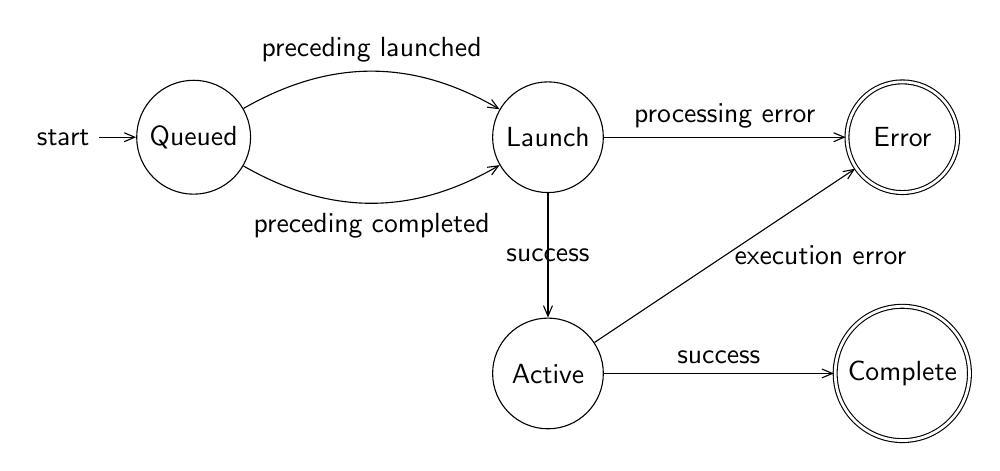
\begin{tikzpicture}
[auto,on grid,node distance=4.5cm,state/.style={circle,draw,minimum size=40pt}]
   \node[state,initial]                 (s0) {Queued};
   \node[state,right=4.5cm of s0]       (s1) {Launch};
   \node[state,below=3cm of s1]       (s2) {Active};
   \node[state,accepting,double distance=1pt,right=of s1]   (s3) {Error};
   \node[state,accepting,double distance=1pt,right=of s2]   (s4) {Complete};
   \path[->]
     (s0) edge[bend right]  node[below] {preceding completed} (s1)
          edge[bend left] node[above]{preceding launched} (s1)
     (s1) edge  node {processing error} (s3)
          edge  node[anchor=center] {success} (s2)
     (s2) edge  node{success} (s4)
          edge  node[right]{execution error} (s3)
     ;
\end{tikzpicture}
  \centering
  \caption{Packet State Diagram}
  \label{fig:packetstate}
\end{figure}

\begin{description}[itemsep=1pt,leftmargin=0cm, labelindent=0cm]
\item[Queued] The queued state means that the format of the packet is not
  \hsaref{HSA_AQL_PACKET_FORMAT_ALWAYS_RESERVED} nor
  \hsaref{HSA_AQL_PACKET_FORMAT_INVALID}.  If the \reffld{barrier} bit is set,
  the transition to launch state occurs after all the preceding kernels have
  completed execution. If the \reffld{barrier} bit is not set, then the
  transition to launch state occurs after the preceding kernels have completed
  their launch phase.

\item[Launch] The launch state indicates processing of the packet, but not
  execution of a task. This phase finalizes by applying an acquire memory fence.
  If an error is detected during launch, the queue is set into an error state
  and the event callback associated with the queue (if present) is invoked. The
  runtime passes an error status to the callback that indicates the source of
  the problem.  The flag \hsaref{HSA_STATUS_ERROR_INVALID_PACKET_FORMAT}
  indicates that an AQL packet is malformed.

\item[Active] The active state means that the kernel encoded by the packet
  has started execution. If an error is detected during this phase, a release
  fence is applied to the packet and its completion signal (if present) is
  assigned a negative value.

\item[Error] The error state means that an error was encountered during the
  launch or active phases.

\item[Complete] The complete state means that a memory release fence has been
  applied and the completion signal (if present) decremented.
\end{description}

\subsubsection{Memory information}

If the kernel being dispatched uses private or group segments, the HSA runtime
requires the application to specify the sizes of the segments in the Dispatch
packet. Manually calculating this information is not feasible and requires
visual inspection of the input program, which itself may have been generated by
a higher-level compiler. For this reason, the user must rely on the finalizer to
get the corresponding segment sizes. For more information on determining segment
sizes, refer to Section~\ref{finalizerchapter}.

Another kind of HSA segment is the kernarg segment, used to pass arguments into
a kernel. The application populates the \reffld{kernarg_address} field of the
Dispatch packet with the address of a buffer of kernarg memory previously
allocated. The buffer contains the
actual parameters passed to the kernel being dispatched.
  
\subsection{Agent Dispatch packet}\label{agent-packet}

Agent Dispatch packets dispatch jobs to HSA agents. The HSA API defines type
\hsaref{hsa_aql_agent_dispatch_packet_t} to represent Agent Dispatch packets.
The states and state transitions for Agent Dispatch packets is identical to that
of Dispatch packets.

\subsection{Barrier packet}\label{barrier-packet}

The Barrier packet \hsaref{hsa_aql_barrier_packet_t} allows an application to
specify up to five dependencies as \hsaref{hsa_signal_handle_t} objects and
requires the HSA Packet Processor to resolve those dependencies before proceeding.
The Barrier packet is a blocking packet in the sense that the processing of the
Barrier packet completes the packet. This is unlike a Dispatch packet whose
completion may occur at some future time after the packet has finished
processing.

The HSA Packet Processor will not launch any further packets until the Barrier
packet is complete. The execution phase for the Barrier packet completes when
either of these two conditions have been met:
\begin{itemize}
\item Any of the dependent signals have been observed with a negative value
  after the Barrier packet launched, in which case the HSA Packet
  Processor assigns an error value to the \reffld{completion_signal} .
\item All of the dependent signals have been observed with the value 0 after
  the Barrier packet launched (note that it is not required that all dependent
  signals are observed to be 0 at the same time).
\end{itemize}

As stated above, if any of the dependent signals have been assigned a negative
value, the Barrier packet will indicate failure in its completion signal. The
HSA Packet Processor assigns an error (negative) value to the
\reffld{completion_signal}.  For more information, refer to
Section~\ref{sec:signals}.

The state diagram of the Barrier packet is identical to that shown for Dispatch
packets. However, each state might cause a different set of actions:
\begin{itemize}
\item No memory fence is applied in the launch phase.
\item In the active phase, instead of executing a kernel, the packet waits for
  all the conditions to be met.
\item No action is performed in the completion phase.
\end{itemize}

\subsection{API}
\makeatletter{}

\subsubsection{hsa_\-aql_\-packet_\-format_\-t}
\vspace{-2mm}\noindent\begin{tcolorbox}[breakable,nobeforeafter,arc=0mm,colframe=white,colback=lightgray,left=0mm]
enum \hypertarget{group__aql_1ga21e03ac6edb26e457468af5fe501b7ad}{\textbf{hsa_\-aql_\-packet_\-format_\-t}}
\end{tcolorbox}
Packet type.

\noindent\textbf{Values}\\[-5mm]
\begin{longtable}{@{\hspace{2em}}p{\linewidth-2em}}
\hspace{-2em}\hypertarget{group__aql_1gga21e03ac6edb26e457468af5fe501b7adaaa022c87937de2531388a681182e4d36}{\refenu{HSA_\-AQL_\-PACKET_\-FORMAT_\-ALWAYS_\-RESERVED}} = 0\\Initial format of a packets when the queue is created. Always reserved packet have never been assigned to the packet processor. From a functional view always reserved packets are equivalent to invalid packets. All queues support this packet format.\\[2mm]
\hspace{-2em}\hypertarget{group__aql_1gga21e03ac6edb26e457468af5fe501b7adadc0bb64d5b0037718e716d57f6befb6a}{\refenu{HSA_\-AQL_\-PACKET_\-FORMAT_\-INVALID}} = 1\\The packet slot has been processed in the past, and has not been reassigned to the packet processor (is available). All queues support this packet format.\\[2mm]
\hspace{-2em}\hypertarget{group__aql_1gga21e03ac6edb26e457468af5fe501b7ada90d2a5dbd40f372f777402c83edf9d86}{\refenu{HSA_\-AQL_\-PACKET_\-FORMAT_\-DISPATCH}} = 2\\Packet used by HSA agents for dispatching jobs to HSA components. Not all queues support packets of this type (see \hyperlink{group__queue_1ga1145b01f6d9e2670179a22c92db39413}{hsa_\-queue_\-feature_\-t}).\\[2mm]
\hspace{-2em}\hypertarget{group__aql_1gga21e03ac6edb26e457468af5fe501b7adadaf10ccf48d374dfa87b7ad237a1788d}{\refenu{HSA_\-AQL_\-PACKET_\-FORMAT_\-BARRIER}} = 3\\Packet used by HSA agents to delay processing of subsequent packets, and to express complex dependencies between multiple packets. All queues support this packet format.\\[2mm]
\hspace{-2em}\hypertarget{group__aql_1gga21e03ac6edb26e457468af5fe501b7ada5189936e5f67be9e3463465aed69b008}{\refenu{HSA_\-AQL_\-PACKET_\-FORMAT_\-AGENT_\-DISPATCH}} = 4\\Packet used by HSA agents for dispatching jobs to HSA agents. Not all queues support packets of this type (see \hyperlink{group__queue_1ga1145b01f6d9e2670179a22c92db39413}{hsa_\-queue_\-feature_\-t}).
\end{longtable}

\subsubsection{hsa_\-fence_\-scope_\-t}
\vspace{-2mm}\noindent\begin{tcolorbox}[breakable,nobeforeafter,arc=0mm,colframe=white,colback=lightgray,left=0mm]
enum \hypertarget{group__aql_1ga6c1a86878de5b0f980202ad7e4e8d42a}{\textbf{hsa_\-fence_\-scope_\-t}}
\end{tcolorbox}
Scope of the memory fence operation associated with a packet.

\noindent\textbf{Values}\\[-5mm]
\begin{longtable}{@{\hspace{2em}}p{\linewidth-2em}}
\hspace{-2em}\hypertarget{group__aql_1gga6c1a86878de5b0f980202ad7e4e8d42aa5dc7b942cd56f91094a088435027be2c}{\refenu{HSA_\-FENCE_\-SCOPE_\-NONE}} = 0\\No scope. Only valid for barrier packets.\\[2mm]
\hspace{-2em}\hypertarget{group__aql_1gga6c1a86878de5b0f980202ad7e4e8d42aa9818589db02bc7c0639652eccd64c95d}{\refenu{HSA_\-FENCE_\-SCOPE_\-COMPONENT}} = 1\\The fence is applied with component scope for the global segment.\\[2mm]
\hspace{-2em}\hypertarget{group__aql_1gga6c1a86878de5b0f980202ad7e4e8d42aa6ecb203c10f12ec4bcf475d527c3a870}{\refenu{HSA_\-FENCE_\-SCOPE_\-SYSTEM}} = 2\\The fence is applied with system scope for the global segment.
\end{longtable}

\subsubsection{hsa_\-aql_\-packet_\-header_\-t}
\vspace{-2mm}\noindent\begin{tcolorbox}[breakable,nobeforeafter,arc=0mm,colframe=white,colback=lightgray,left=0mm]
typedef struct  hsa_aql_packet_header_s \{
\vspace{-3.5mm}\begin{longtable}{@{}p{\textwidth}}
\hspace{1.7em}\hyperlink{group__aql_1ga21e03ac6edb26e457468af5fe501b7ad}{hsa_\-aql_\-packet_\-format_\-t} \reffld{format} : 8;\\
\hspace{1.7em}uint16_\-t \reffld{barrier} : 1;\\
\hspace{1.7em}\hyperlink{group__aql_1ga6c1a86878de5b0f980202ad7e4e8d42a}{hsa_\-fence_\-scope_\-t} \reffld{acquire_\-fence_\-scope} : 2;\\
\hspace{1.7em}\hyperlink{group__aql_1ga6c1a86878de5b0f980202ad7e4e8d42a}{hsa_\-fence_\-scope_\-t} \reffld{release_\-fence_\-scope} : 2;\\
\hspace{1.7em}uint16_\-t \reffld{reserved} : 3;\\
\}  \hypertarget{group__aql_1ga92558e047d003985bae2558febd3dd40}{\textbf{hsa_\-aql_\-packet_\-header_\-t}}
\end{longtable}

\end{tcolorbox}
AQL packet header.

\noindent\textbf{Data Fields}\\[-6mm]
\begin{longtable}{@{}>{\hangindent=2em}p{\textwidth}}
\reffld{format}\\\hspace{2em}Packet type.\\[2mm]
\reffld{barrier}\\\hspace{2em}If set, the processing of the current packet only launches when all preceding packets (within the same queue) are complete.\\[2mm]
\reffld{acquire_\-fence_\-scope}\\\hspace{2em}Determines the scope and type of the memory fence operation applied before the packet enters the active phase.\\[2mm]
\reffld{release_\-fence_\-scope}\\\hspace{2em}Determines the scope and type of the memory fence operation applied after kernel completion but before the packet is completed.\\[2mm]
\reffld{reserved}\\\hspace{2em}Must be a value of 0.
\end{longtable}



\subsubsection{hsa_\-aql_\-dispatch_\-packet_\-t}
\vspace{-2mm}\noindent\begin{tcolorbox}[breakable,nobeforeafter,arc=0mm,colframe=white,colback=lightgray,left=0mm]
typedef struct  hsa_aql_dispatch_packet_s \{
\vspace{-3.5mm}\begin{longtable}{@{}p{\textwidth}}
\hspace{1.7em}\hyperlink{group__aql_1ga92558e047d003985bae2558febd3dd40}{hsa_\-aql_\-packet_\-header_\-t} \reffld{header};\\
\hspace{1.7em}uint16_\-t \reffld{dimensions} : 2;\\
\hspace{1.7em}uint16_\-t \reffld{reserved} : 14;\\
\hspace{1.7em}uint16_\-t \reffld{workgroup_\-size_\-x};\\
\hspace{1.7em}uint16_\-t \reffld{workgroup_\-size_\-y};\\
\hspace{1.7em}uint16_\-t \reffld{workgroup_\-size_\-z};\\
\hspace{1.7em}uint16_\-t \reffld{reserved2};\\
\hspace{1.7em}uint32_\-t \reffld{grid_\-size_\-x};\\
\hspace{1.7em}uint32_\-t \reffld{grid_\-size_\-y};\\
\hspace{1.7em}uint32_\-t \reffld{grid_\-size_\-z};\\
\hspace{1.7em}uint32_\-t \reffld{private_\-segment_\-size_\-bytes};\\
\hspace{1.7em}uint32_\-t \reffld{group_\-segment_\-size_\-bytes};\\
\hspace{1.7em}uint64_\-t \reffld{kernel_\-object_\-address};\\
\hspace{1.7em}uint64_\-t \reffld{kernarg_\-address};\\
\hspace{1.7em}uint64_\-t \reffld{reserved3};\\
\hspace{1.7em}\hyperlink{group__signals_1ga6592c136d70853d855bc11d9efdbf534}{hsa_\-signal_\-handle_\-t} \reffld{completion_\-signal};\\
\}  \hypertarget{group__aql_1gab3d5ded5ac53f70931768468c0c0cfd6}{\textbf{hsa_\-aql_\-dispatch_\-packet_\-t}}
\end{longtable}

\end{tcolorbox}
AQL dispatch packet.

\noindent\textbf{Data Fields}\\[-6mm]
\begin{longtable}{@{}>{\hangindent=2em}p{\textwidth}}
\reffld{header}\\\hspace{2em}Packet header.\\[2mm]
\reffld{dimensions}\\\hspace{2em}Number of dimensions specified in the grid size. Valid values are 1, 2, or 3.\\[2mm]
\reffld{reserved}\\\hspace{2em}Reserved, must be a value of 0.\\[2mm]
\reffld{workgroup_\-size_\-x}\\\hspace{2em}X dimension of work-group (measured in work-items).\\[2mm]
\reffld{workgroup_\-size_\-y}\\\hspace{2em}Y dimension of work-group (measured in work-items).\\[2mm]
\reffld{workgroup_\-size_\-z}\\\hspace{2em}Z dimension of work-group (measured in work-items).\\[2mm]
\reffld{reserved2}\\\hspace{2em}Reserved. Must be a value of 0.\\[2mm]
\reffld{grid_\-size_\-x}\\\hspace{2em}X dimension of grid (measured in work-items).\\[2mm]
\reffld{grid_\-size_\-y}\\\hspace{2em}Y dimension of grid (measured in work-items).\\[2mm]
\reffld{grid_\-size_\-z}\\\hspace{2em}Z dimension of grid (measured in work-items).\\[2mm]
\reffld{private_\-segment_\-size_\-bytes}\\\hspace{2em}Size (in bytes) of private memory allocation request (per work-item).\\[2mm]
\reffld{group_\-segment_\-size_\-bytes}\\\hspace{2em}Size (in bytes) of group memory allocation request (per work-group).\\[2mm]
\reffld{kernel_\-object_\-address}\\\hspace{2em}Address of an object in memory that includes an implementation-defined executable ISA image for the kernel.\\[2mm]
\reffld{kernarg_\-address}\\\hspace{2em}Address of memory containing kernel arguments.\\[2mm]
\reffld{reserved3}\\\hspace{2em}Reserved. Must be a value of 0.\\[2mm]
\reffld{completion_\-signal}\\\hspace{2em}Signaling object handle used to indicate completion of the job.
\end{longtable}



\subsubsection{hsa_\-aql_\-agent_\-dispatch_\-packet_\-t}
\vspace{-2mm}\noindent\begin{tcolorbox}[breakable,nobeforeafter,arc=0mm,colframe=white,colback=lightgray,left=0mm]
typedef struct  hsa_aql_agent_dispatch_packet_s \{
\vspace{-3.5mm}\begin{longtable}{@{}p{\textwidth}}
\hspace{1.7em}\hyperlink{group__aql_1ga92558e047d003985bae2558febd3dd40}{hsa_\-aql_\-packet_\-header_\-t} \reffld{header};\\
\hspace{1.7em}uint16_\-t \reffld{type};\\
\hspace{1.7em}uint32_\-t \reffld{reserved2};\\
\hspace{1.7em}uint64_\-t \reffld{return_\-location};\\
\hspace{1.7em}uint64_\-t \reffld{arg}[4];\\
\hspace{1.7em}uint64_\-t \reffld{reserved3};\\
\hspace{1.7em}\hyperlink{group__signals_1ga6592c136d70853d855bc11d9efdbf534}{hsa_\-signal_\-handle_\-t} \reffld{completion_\-signal};\\
\}  \hypertarget{group__aql_1ga07dc7a6c787b5bee6e3f0b8b79586109}{\textbf{hsa_\-aql_\-agent_\-dispatch_\-packet_\-t}}
\end{longtable}

\end{tcolorbox}
Agent dispatch packet.

\noindent\textbf{Data Fields}\\[-6mm]
\begin{longtable}{@{}>{\hangindent=2em}p{\textwidth}}
\reffld{header}\\\hspace{2em}Packet header.\\[2mm]
\reffld{type}\\\hspace{2em}The function to be performed by the destination HSA Agent. The type value is split into the following ranges: 0x0000:0x3FFF (vendor specific), 0x4000:0x7FFF (HSA runtime) 0x8000:0xFFFF (user registered function).\\[2mm]
\reffld{reserved2}\\\hspace{2em}Reserved. Must be a value of 0.\\[2mm]
\reffld{return_\-location}\\\hspace{2em}Pointer to location to store the function return value(s) in.\\[2mm]
\reffld{arg}\\\hspace{2em}64-bit direct or indirect arguments.\\[2mm]
\reffld{reserved3}\\\hspace{2em}Reserved. Must be a value of 0.\\[2mm]
\reffld{completion_\-signal}\\\hspace{2em}Signaling object handle used to indicate completion of the job.
\end{longtable}



\subsubsection{hsa_\-aql_\-barrier_\-packet_\-t}
\vspace{-2mm}\noindent\begin{tcolorbox}[breakable,nobeforeafter,arc=0mm,colframe=white,colback=lightgray,left=0mm]
typedef struct  hsa_aql_barrier_packet_s \{
\vspace{-3.5mm}\begin{longtable}{@{}p{\textwidth}}
\hspace{1.7em}\hyperlink{group__aql_1ga92558e047d003985bae2558febd3dd40}{hsa_\-aql_\-packet_\-header_\-t} \reffld{header};\\
\hspace{1.7em}uint16_\-t \reffld{reserved2};\\
\hspace{1.7em}uint32_\-t \reffld{reserved3};\\
\hspace{1.7em}\hyperlink{group__signals_1ga6592c136d70853d855bc11d9efdbf534}{hsa_\-signal_\-handle_\-t} \reffld{dep_\-signal}[5];\\
\hspace{1.7em}uint64_\-t \reffld{reserved4};\\
\hspace{1.7em}\hyperlink{group__signals_1ga6592c136d70853d855bc11d9efdbf534}{hsa_\-signal_\-handle_\-t} \reffld{completion_\-signal};\\
\}  \hypertarget{group__aql_1ga8e5ebbeffbf5af1ece8db9ef27c14715}{\textbf{hsa_\-aql_\-barrier_\-packet_\-t}}
\end{longtable}

\end{tcolorbox}
Barrier packet.

\noindent\textbf{Data Fields}\\[-6mm]
\begin{longtable}{@{}>{\hangindent=2em}p{\textwidth}}
\reffld{header}\\\hspace{2em}Packet header.\\[2mm]
\reffld{reserved2}\\\hspace{2em}Reserved. Must be a value of 0.\\[2mm]
\reffld{reserved3}\\\hspace{2em}Reserved. Must be a value of 0.\\[2mm]
\reffld{dep_\-signal}\\\hspace{2em}Array of dependent signal objects.\\[2mm]
\reffld{reserved4}\\\hspace{2em}Reserved. Must be a value of 0.\\[2mm]
\reffld{completion_\-signal}\\\hspace{2em}Signaling object handle used to indicate completion of the job.
\end{longtable}

 

\section{Memory}\label{memory}

One of the key features of HSA is its ability to share global pointers between
the host application and code executing on the component. This ability means
that an application can directly pass a pointer to memory allocated on the host
to a kernel function dispatched to a component.

When a buffer created in the host is also accessed by a component, programmers
are encouraged to \emph{register} the corresponding address range beforehand by
using the \hsaref{hsa_memory_register} API. While kernels running on HSA devices
can access any memory pointer allocated by means of standard libraries (for
example, malloc in the C language), registering the buffer might result on
improved access performance.  When an HSA program no longer needs to access a
registered buffer in a device, the application should deregister that virtual
address range by using the appropriate HSA core API invocation.

The kernarg memory that AQL packet points to (see Section~\ref{sec:aql}) holds
information about any arguments required to execute AQL dispatch on a HSA
component. While any system memory may be used for kernarg memory,
implementation/platform specific optimizations are possible if HSA core runtime
provided API are utilized for allocating and copying to the allocated kernarg
memory.


\subsection{API}
\makeatletter{}

\subsubsection{hsa_\-region_\-t}
\vspace{-2mm}\noindent\begin{tcolorbox}[nobeforeafter,arc=0mm,colframe=white,colback=lightgray,left=0mm]
typedef uint64_\-t  \hypertarget{group__memory_1gaa5f6311c53cbe299caebef621e060588}{\textbf{hsa_\-region_\-t}}
\end{tcolorbox}
A memory region represents a virtual memory interval that is visible to a particular agent, and contains properties about how memory is accessed or allocated from that agent.
\\

\subsubsection{hsa_\-segment_\-t}
\vspace{-2mm}\noindent\begin{tcolorbox}[breakable,nobeforeafter,arc=0mm,colframe=white,colback=lightgray,left=0mm]
enum \hypertarget{group__memory_1ga9aa2ffad72549139936d37692a4214dd}{\textbf{hsa_\-segment_\-t}}
\end{tcolorbox}
Memory segments.

\noindent\textbf{Values}\\[-5mm]
\begin{longtable}{@{\hspace{2em}}p{\linewidth-2em}}
\hspace{-2em}\hypertarget{group__memory_1gga9aa2ffad72549139936d37692a4214dda0488a507ac10e730a5da4c7e88c9708b}{\refenu{HSA_\-SEGMENT_\-GLOBAL}} = 1\\Global segment.\\[2mm]
\hspace{-2em}\hypertarget{group__memory_1gga9aa2ffad72549139936d37692a4214dda8973c2316a8b2247b8a2a2f2546cde38}{\refenu{HSA_\-SEGMENT_\-PRIVATE}} = 2\\Private segment.\\[2mm]
\hspace{-2em}\hypertarget{group__memory_1gga9aa2ffad72549139936d37692a4214ddad3e8c2fe02eb7e9febdacb51dff74d5e}{\refenu{HSA_\-SEGMENT_\-GROUP}} = 4\\Group segment.\\[2mm]
\hspace{-2em}\hypertarget{group__memory_1gga9aa2ffad72549139936d37692a4214dda79388d7547c31b8b90ada3f6e5470603}{\refenu{HSA_\-SEGMENT_\-KERNARG}} = 8\\Kernarg segment.\\[2mm]
\hspace{-2em}\hypertarget{group__memory_1gga9aa2ffad72549139936d37692a4214dda9a30a39c5916dd3e21f896442a71357e}{\refenu{HSA_\-SEGMENT_\-READONLY}} = 16\\Readonly segment.\\[2mm]
\hspace{-2em}\hypertarget{group__memory_1gga9aa2ffad72549139936d37692a4214dda9f392bce1a9ab02d6a372823a4ffb1fb}{\refenu{HSA_\-SEGMENT_\-IMAGE}} = 32\\Image segment.
\end{longtable}

\subsubsection{hsa_\-region_\-info_\-t}
\vspace{-2mm}\noindent\begin{tcolorbox}[breakable,nobeforeafter,arc=0mm,colframe=white,colback=lightgray,left=0mm]
enum \hypertarget{group__memory_1gad35755078ff15f645c6c25e7f7ef2707}{\textbf{hsa_\-region_\-info_\-t}}
\end{tcolorbox}
Attributes of a memory region.

\noindent\textbf{Values}\\[-5mm]
\begin{longtable}{@{\hspace{2em}}p{\linewidth-2em}}
\hspace{-2em}\hypertarget{group__memory_1ggad35755078ff15f645c6c25e7f7ef2707aa244eb381cc0c1abc669faa36218c096}{\refenu{HSA_\-REGION_\-INFO_\-BASE_\-ADDRESS}} \\Base (starting) address. The type of this attribute is void*.\\[2mm]
\hspace{-2em}\hypertarget{group__memory_1ggad35755078ff15f645c6c25e7f7ef2707a09403f5c83497726504523694b3e86b6}{\refenu{HSA_\-REGION_\-INFO_\-SIZE}} \\Size, in bytes. The type of this attribute is size_\-t.\\[2mm]
\hspace{-2em}\hypertarget{group__memory_1ggad35755078ff15f645c6c25e7f7ef2707ab7bb10ceec7634e32c7ad29e6b4a31a0}{\refenu{HSA_\-REGION_\-INFO_\-NODE}} \\NUMA node associated with this region. The type of this attribute is \hyperlink{group__agentinfo_1gaef5077ca9988ea43e37c17dea3884333}{hsa_\-node_\-t}\\[2mm]
\hspace{-2em}\hypertarget{group__memory_1ggad35755078ff15f645c6c25e7f7ef2707a46d6f8d59f25ba5a4c4200e836109043}{\refenu{HSA_\-REGION_\-INFO_\-MAX_\-ALLOCATION_\-SIZE}} \\Maximum allocation size in this region, in bytes. A value of 0 indicates that the host cannot allocate memory in the region. The type of this attribute is size_\-t.\\[2mm]
\hspace{-2em}\hypertarget{group__memory_1ggad35755078ff15f645c6c25e7f7ef2707ab2701b5deebcf46596e8f070f6ef27b6}{\refenu{HSA_\-REGION_\-INFO_\-SEGMENT}} \\Segment where the memory in the region can be used. The type of this attribute is \hyperlink{group__memory_1ga9aa2ffad72549139936d37692a4214dd}{hsa_\-segment_\-t}.\\[2mm]
\hspace{-2em}\hypertarget{group__memory_1ggad35755078ff15f645c6c25e7f7ef2707a77389057885a6a331863536fe4c66a5c}{\refenu{HSA_\-REGION_\-INFO_\-BANDWIDTH}} \\Peak bandwidth for component access, in Mbs per second. The type of this attribute is uint32_\-t\\[2mm]
\hspace{-2em}\hypertarget{group__memory_1ggad35755078ff15f645c6c25e7f7ef2707a71b24dd1af185b70c275b377e3e51989}{\refenu{HSA_\-REGION_\-INFO_\-CACHED}} \\Cache levels that cache data in the region. The type of this attribute is bool[4].
\end{longtable}

\subsubsection{hsa_\-region_\-get_\-info}
\vspace{-2mm}\noindent\begin{tcolorbox}[breakable,nobeforeafter,colframe=white,colback=lightgray,left=0mm]
\hyperlink{group__status_1gad755322e7ff95456520e8abdbe90d225}{hsa_\-status_\-t} \index[api]{hsa_\-region_\-get_\-info}\hypertarget{group__memory_1gaad0ab0056cfee2e5a99270490b942a28}{\textbf{hsa_\-region_\-get_\-info}}(
\vspace{-3.5mm}\begin{longtable}{@{}p{\textwidth}}
\hspace{1.7em}\hyperlink{group__memory_1gaa5f6311c53cbe299caebef621e060588}{hsa_\-region_\-t} \hsaarg{region},\\
\hspace{1.7em}\hyperlink{group__memory_1gad35755078ff15f645c6c25e7f7ef2707}{hsa_\-region_\-info_\-t} \hsaarg{attribute},\\
\hspace{1.7em}void * \hsaarg{value})\end{longtable}

\end{tcolorbox}
Get the current value of an attribute of a region.

\noindent\textbf{Parameters}\\[-6mm]
\noindent\begin{longtable}{@{}>{\hangindent=2em}p{\textwidth}}
\hsaarg{region}\\\hspace{2em}(in) A valid region.\\[2mm]
\hsaarg{attribute}\\\hspace{2em}(in) Attribute to query.\\[2mm]
\hsaarg{value}\\\hspace{2em}(out) Pointer to a user-allocated buffer where to store the value of the attribute. If the buffer passed by the application is not large enough to hold the value of \textit{attribute}, the behavior is undefined.
\end{longtable}
\vspace{-5mm}\noindent\textbf{Return Values}\\[-6mm]
\noindent\begin{longtable}{@{}>{\hangindent=2em}p{\linewidth}}
\hyperlink{group__status_1ggad755322e7ff95456520e8abdbe90d225ae382ea0c9c05cce5a60d0317375159cc}{HSA_\-STATUS_\-SUCCESS}\\\hspace{2em}The function has been executed successfully.\\[2mm]
\hyperlink{group__status_1ggad755322e7ff95456520e8abdbe90d225a34ea59ade5bfce95eee935238a99f5b5}{HSA_\-STATUS_\-ERROR_\-NOT_\-INITIALIZED}\\\hspace{2em}The runtime has not been initialized.\\[2mm]
\hyperlink{group__status_1ggad755322e7ff95456520e8abdbe90d225ad63594ac02edec7ae7aa7722c11afcd9}{HSA_\-STATUS_\-ERROR_\-INVALID_\-REGION}\\\hspace{2em}If the region is invalid.\\[2mm]
\hyperlink{group__status_1ggad755322e7ff95456520e8abdbe90d225ac7d3651f75107d2a6a8ba3b25683c030}{HSA_\-STATUS_\-ERROR_\-INVALID_\-ARGUMENT}\\\hspace{2em}If \textit{attribute} is not a valid region attribute, or \textit{value} is NULL.
\end{longtable}
 


\subsubsection{hsa_\-agent_\-iterate_\-regions}
\vspace{-2mm}\noindent\begin{tcolorbox}[breakable,nobeforeafter,colframe=white,colback=lightgray,left=0mm]
\hyperlink{group__status_1gad755322e7ff95456520e8abdbe90d225}{hsa_\-status_\-t} \index[api]{hsa_\-agent_\-iterate_\-regions}\hypertarget{group__memory_1gad595a460e2867a134ec90de63589c0eb}{\textbf{hsa_\-agent_\-iterate_\-regions}}(
\vspace{-3.5mm}\begin{longtable}{@{}p{\textwidth}}
\hspace{1.7em}\hyperlink{group__agentinfo_1ga27393931438432bb42772bc10f5d4941}{hsa_\-agent_\-t} \hsaarg{agent},\\
\hspace{1.7em}\hyperlink{group__status_1gad755322e7ff95456520e8abdbe90d225}{hsa_\-status_\-t}(*)(\hyperlink{group__memory_1gaa5f6311c53cbe299caebef621e060588}{hsa_\-region_\-t} region, void *data) \hsaarg{callback},\\
\hspace{1.7em}void * \hsaarg{data})\end{longtable}

\end{tcolorbox}
Iterate over the memory regions that are visible to an agent, and invoke an application-defined callback on every iteration.

\noindent\textbf{Parameters}\\[-6mm]
\noindent\begin{longtable}{@{}>{\hangindent=2em}p{\textwidth}}
\hsaarg{agent}\\\hspace{2em}(in) A valid agent.\\[2mm]
\hsaarg{callback}\\\hspace{2em}(in) Callback to be invoked once per region that is visible from the agent.\\[2mm]
\hsaarg{data}\\\hspace{2em}(in) Application data that is passed to \textit{callback} on every iteration. Can be NULL.
\end{longtable}
\vspace{-5mm}\noindent\textbf{Return Values}\\[-6mm]
\noindent\begin{longtable}{@{}>{\hangindent=2em}p{\linewidth}}
\hyperlink{group__status_1ggad755322e7ff95456520e8abdbe90d225ae382ea0c9c05cce5a60d0317375159cc}{HSA_\-STATUS_\-SUCCESS}\\\hspace{2em}The function has been executed successfully.\\[2mm]
\hyperlink{group__status_1ggad755322e7ff95456520e8abdbe90d225a34ea59ade5bfce95eee935238a99f5b5}{HSA_\-STATUS_\-ERROR_\-NOT_\-INITIALIZED}\\\hspace{2em}The runtime has not been initialized.\\[2mm]
\hyperlink{group__status_1ggad755322e7ff95456520e8abdbe90d225a3a5d835c109c2d0ad5b9c2771e133e5d}{HSA_\-STATUS_\-ERROR_\-INVALID_\-AGENT}\\\hspace{2em}If the agent is invalid.\\[2mm]
\hyperlink{group__status_1ggad755322e7ff95456520e8abdbe90d225ac7d3651f75107d2a6a8ba3b25683c030}{HSA_\-STATUS_\-ERROR_\-INVALID_\-ARGUMENT}\\\hspace{2em}If \textit{callback} is NULL.
\end{longtable}
\vspace{-4mm}\noindent\textbf{Description}\\[1mm]
If \textit{callback} returns a status other than \hyperlink{group__status_1ggad755322e7ff95456520e8abdbe90d225ae382ea0c9c05cce5a60d0317375159cc}{HSA_\-STATUS_\-SUCCESS} for a particular iteration, the traversal stops and the function returns that status value. 


\subsubsection{hsa_\-memory_\-allocate}
\vspace{-2mm}\noindent\begin{tcolorbox}[breakable,nobeforeafter,colframe=white,colback=lightgray,left=0mm]
\hyperlink{group__status_1gad755322e7ff95456520e8abdbe90d225}{hsa_\-status_\-t} \index[api]{hsa_\-memory_\-allocate}\hypertarget{group__memory_1gace14b2b247c35850670793ae6f1f1425}{\textbf{hsa_\-memory_\-allocate}}(
\vspace{-3.5mm}\begin{longtable}{@{}p{\textwidth}}
\hspace{1.7em}\hyperlink{group__memory_1gaa5f6311c53cbe299caebef621e060588}{hsa_\-region_\-t} \hsaarg{region},\\
\hspace{1.7em}size_\-t \hsaarg{size},\\
\hspace{1.7em}size_\-t \hsaarg{alignment},\\
\hspace{1.7em}void ** \hsaarg{ptr})\end{longtable}

\end{tcolorbox}
Allocate a block of memory.

\noindent\textbf{Parameters}\\[-6mm]
\noindent\begin{longtable}{@{}>{\hangindent=2em}p{\textwidth}}
\hsaarg{region}\\\hspace{2em}(in) Region where to allocate memory from.\\[2mm]
\hsaarg{size}\\\hspace{2em}(in) Allocation size, in bytes. Allocation of size 0 is allowed and returns a NULL pointer.\\[2mm]
\hsaarg{alignment}\\\hspace{2em}(in) The alignment size (in bytes) for the base address of the resulting allocation. If the value is zero, no particular alignment will be applied. If the value is not zero, it must be a power of two that is not smaller than sizeof(void*).\\[2mm]
\hsaarg{ptr}\\\hspace{2em}(out) A pointer to the location of where to return the pointer to the base of the allocated region of memory.
\end{longtable}
\vspace{-5mm}\noindent\textbf{Return Values}\\[-6mm]
\noindent\begin{longtable}{@{}>{\hangindent=2em}p{\linewidth}}
\hyperlink{group__status_1ggad755322e7ff95456520e8abdbe90d225ae382ea0c9c05cce5a60d0317375159cc}{HSA_\-STATUS_\-SUCCESS}\\\hspace{2em}The function has been executed successfully.\\[2mm]
\hyperlink{group__status_1ggad755322e7ff95456520e8abdbe90d225a34ea59ade5bfce95eee935238a99f5b5}{HSA_\-STATUS_\-ERROR_\-NOT_\-INITIALIZED}\\\hspace{2em}The runtime has not been initialized.\\[2mm]
\hyperlink{group__status_1ggad755322e7ff95456520e8abdbe90d225a1a77fcf36d0d140874c4361ab093eff7}{HSA_\-STATUS_\-ERROR_\-OUT_\-OF_\-RESOURCES}\\\hspace{2em}If there is a failure in allocation. This error may also occur when the core runtime library needs to spawn threads or create internal OS-specific events.\\[2mm]
\hyperlink{group__status_1ggad755322e7ff95456520e8abdbe90d225ac7d3651f75107d2a6a8ba3b25683c030}{HSA_\-STATUS_\-ERROR_\-INVALID_\-ARGUMENT}\\\hspace{2em}If \textit{alignment} is not a power of two, or \textit{alignment} is smaller than sizeof(void*) but not 0, or \textit{ptr} is NULL.
\end{longtable}
 


\subsubsection{hsa_\-memory_\-free}
\vspace{-2mm}\noindent\begin{tcolorbox}[breakable,nobeforeafter,colframe=white,colback=lightgray,left=0mm]
\hyperlink{group__status_1gad755322e7ff95456520e8abdbe90d225}{hsa_\-status_\-t} \index[api]{hsa_\-memory_\-free}\hypertarget{group__memory_1gaf968e8053981351ec0b16a04aeb51a8e}{\textbf{hsa_\-memory_\-free}}(
\vspace{-3.5mm}\begin{longtable}{@{}p{\textwidth}}
\hspace{1.7em}void * \hsaarg{ptr})\end{longtable}

\end{tcolorbox}
Deallocate a block of memory previously allocated using \hyperlink{group__memory_1gace14b2b247c35850670793ae6f1f1425}{\reffun{hsa_\-memory_\-allocate}}.

\noindent\textbf{Parameters}\\[-6mm]
\noindent\begin{longtable}{@{}>{\hangindent=2em}p{\textwidth}}
\hsaarg{ptr}\\\hspace{2em}(in) Pointer to a memory block. If \textit{ptr} is NULL, no action is performed.
\end{longtable}
\vspace{-5mm}\noindent\textbf{Return Values}\\[-6mm]
\noindent\begin{longtable}{@{}>{\hangindent=2em}p{\linewidth}}
\hyperlink{group__status_1ggad755322e7ff95456520e8abdbe90d225ae382ea0c9c05cce5a60d0317375159cc}{HSA_\-STATUS_\-SUCCESS}\\\hspace{2em}The function has been executed successfully.\\[2mm]
\hyperlink{group__status_1ggad755322e7ff95456520e8abdbe90d225a34ea59ade5bfce95eee935238a99f5b5}{HSA_\-STATUS_\-ERROR_\-NOT_\-INITIALIZED}\\\hspace{2em}The runtime has not been initialized.
\end{longtable}
 


\subsubsection{hsa_\-memory_\-copy}
\vspace{-2mm}\noindent\begin{tcolorbox}[breakable,nobeforeafter,colframe=white,colback=lightgray,left=0mm]
\hyperlink{group__status_1gad755322e7ff95456520e8abdbe90d225}{hsa_\-status_\-t} \index[api]{hsa_\-memory_\-copy}\hypertarget{group__memory_1ga471ef2f21b50ea21f2cf07ebac77ff32}{\textbf{hsa_\-memory_\-copy}}(
\vspace{-3.5mm}\begin{longtable}{@{}p{\textwidth}}
\hspace{1.7em}void * \hsaarg{dst},\\
\hspace{1.7em}const void * \hsaarg{src},\\
\hspace{1.7em}size_\-t \hsaarg{size})\end{longtable}

\end{tcolorbox}
Copy block of memory.

\noindent\textbf{Parameters}\\[-6mm]
\noindent\begin{longtable}{@{}>{\hangindent=2em}p{\textwidth}}
\hsaarg{dst}\\\hspace{2em}(out) A valid pointer to the destination array where the content is to be copied.\\[2mm]
\hsaarg{src}\\\hspace{2em}(in) A valid pointer to the source of data to be copied.\\[2mm]
\hsaarg{size}\\\hspace{2em}(in) Number of bytes to copy. If \textit{size} is 0, no copy is performed and the function returns success.
\end{longtable}
\vspace{-5mm}\noindent\textbf{Return Values}\\[-6mm]
\noindent\begin{longtable}{@{}>{\hangindent=2em}p{\linewidth}}
\hyperlink{group__status_1ggad755322e7ff95456520e8abdbe90d225ae382ea0c9c05cce5a60d0317375159cc}{HSA_\-STATUS_\-SUCCESS}\\\hspace{2em}The function has been executed successfully.\\[2mm]
\hyperlink{group__status_1ggad755322e7ff95456520e8abdbe90d225a34ea59ade5bfce95eee935238a99f5b5}{HSA_\-STATUS_\-ERROR_\-NOT_\-INITIALIZED}\\\hspace{2em}The runtime has not been initialized.\\[2mm]
\hyperlink{group__status_1ggad755322e7ff95456520e8abdbe90d225ac7d3651f75107d2a6a8ba3b25683c030}{HSA_\-STATUS_\-ERROR_\-INVALID_\-ARGUMENT}\\\hspace{2em}If the source or destination pointers are NULL.
\end{longtable}
\vspace{-4mm}\noindent\textbf{Description}\\[1mm]
Copying a number of bytes larger than the size of the memory regions pointed by \textit{dst} or \textit{src} results in undefined behavior. 


\subsubsection{hsa_\-memory_\-register}
\vspace{-2mm}\noindent\begin{tcolorbox}[breakable,nobeforeafter,colframe=white,colback=lightgray,left=0mm]
\hyperlink{group__status_1gad755322e7ff95456520e8abdbe90d225}{hsa_\-status_\-t} \index[api]{hsa_\-memory_\-register}\hypertarget{group__memory_1gaa4d4efc5ba903ea29587392aa1c8a267}{\textbf{hsa_\-memory_\-register}}(
\vspace{-3.5mm}\begin{longtable}{@{}p{\textwidth}}
\hspace{1.7em}void * \hsaarg{address},\\
\hspace{1.7em}size_\-t \hsaarg{size})\end{longtable}

\end{tcolorbox}
Register memory.

\noindent\textbf{Parameters}\\[-6mm]
\noindent\begin{longtable}{@{}>{\hangindent=2em}p{\textwidth}}
\hsaarg{address}\\\hspace{2em}(in) A pointer to the base of the memory region to be registered. If a NULL pointer is passed, no operation is performed.\\[2mm]
\hsaarg{size}\\\hspace{2em}(in) Requested registration size in bytes. A size of zero is only allowed if \textit{address} is NULL.
\end{longtable}
\vspace{-5mm}\noindent\textbf{Return Values}\\[-6mm]
\noindent\begin{longtable}{@{}>{\hangindent=2em}p{\linewidth}}
\hyperlink{group__status_1ggad755322e7ff95456520e8abdbe90d225ae382ea0c9c05cce5a60d0317375159cc}{HSA_\-STATUS_\-SUCCESS}\\\hspace{2em}The function has been executed successfully.\\[2mm]
\hyperlink{group__status_1ggad755322e7ff95456520e8abdbe90d225a34ea59ade5bfce95eee935238a99f5b5}{HSA_\-STATUS_\-ERROR_\-NOT_\-INITIALIZED}\\\hspace{2em}The runtime has not been initialized.\\[2mm]
\hyperlink{group__status_1ggad755322e7ff95456520e8abdbe90d225a1a77fcf36d0d140874c4361ab093eff7}{HSA_\-STATUS_\-ERROR_\-OUT_\-OF_\-RESOURCES}\\\hspace{2em}If there is a failure in allocating the necessary resources.\\[2mm]
\hyperlink{group__status_1ggad755322e7ff95456520e8abdbe90d225ac7d3651f75107d2a6a8ba3b25683c030}{HSA_\-STATUS_\-ERROR_\-INVALID_\-ARGUMENT}\\\hspace{2em}If \textit{size} is 0 but \textit{address} is not NULL.
\end{longtable}
\vspace{-4mm}\noindent\textbf{Description}\\[1mm]
Registering memory expresses an intention to access (read or write) the passed buffer from a component other than the host. This is a performance hint that allows the runtime implementation to know which buffers will be accessed by some of the components ahead of time.\\[2mm]
Overlapping registrations (including multiple registrations of the same buffer) are allowed. 


\subsubsection{hsa_\-memory_\-deregister}
\vspace{-2mm}\noindent\begin{tcolorbox}[breakable,nobeforeafter,colframe=white,colback=lightgray,left=0mm]
\hyperlink{group__status_1gad755322e7ff95456520e8abdbe90d225}{hsa_\-status_\-t} \index[api]{hsa_\-memory_\-deregister}\hypertarget{group__memory_1ga05508ed130cdd83aeab76db3328a45fc}{\textbf{hsa_\-memory_\-deregister}}(
\vspace{-3.5mm}\begin{longtable}{@{}p{\textwidth}}
\hspace{1.7em}void * \hsaarg{address})\end{longtable}

\end{tcolorbox}
Deregister memory previously registered using \hyperlink{group__memory_1gaa4d4efc5ba903ea29587392aa1c8a267}{\reffun{hsa_\-memory_\-register}}.

\noindent\textbf{Parameters}\\[-6mm]
\noindent\begin{longtable}{@{}>{\hangindent=2em}p{\textwidth}}
\hsaarg{address}\\\hspace{2em}(in) A pointer to the base of the memory region to be deregistered. If a NULL pointer is passed, no operation is performed.
\end{longtable}
\vspace{-5mm}\noindent\textbf{Return Values}\\[-6mm]
\noindent\begin{longtable}{@{}>{\hangindent=2em}p{\linewidth}}
\hyperlink{group__status_1ggad755322e7ff95456520e8abdbe90d225ae382ea0c9c05cce5a60d0317375159cc}{HSA_\-STATUS_\-SUCCESS}\\\hspace{2em}The function has been executed successfully.\\[2mm]
\hyperlink{group__status_1ggad755322e7ff95456520e8abdbe90d225a8b2f486dd206aa5545e8b0f2c1e2a568}{HSA_\-STATUS_\-ERROR_\-NOT_\-REGISTERED}\\\hspace{2em}If the pointer has not been registered before.
\end{longtable}
\vspace{-4mm}\noindent\textbf{Description}\\[1mm]
Deregistration must be performed using an address that was previously registered. In the event that deregistration is performed on an address that has been used in multiple registrations, the smallest of the registrations is deregistered. 
 




\section{Extensions to the Core Runtime API}\label{extensions}

Extensions to the Core API can be optional (multi-vendor) or vendor
specific. The difference is in the naming scheme used for the symbols (defines,
structures, functions, etc.) associated with the function:

\begin{itemize}
\item Symbols for multi-vendor extensions defined in the global namespace must
  use the \emph{hsa_ext_} prefix in their identifiers.
\item Symbols for single vendor extensions defined in the global namespace must
  use the \emph{hsa_svext_VENDOR_} prefix in their identifiers. Company names
  must be registered with the HSA Foundation, must be unique, and may be
  abbreviated to improve the readability of the symbols.
\end{itemize}

Any constant definitions in the extension (\#define or enumeration values) use
the same naming convention, except using all capital letters.

The symbols for all vendor extensions (both single-vendor and multi-vendor) are
captured in the file {\bf hsa/vendor_extensions.h}. This file is maintained by
the HSA Foundation. This file includes the enumeration \hsaref{hsa_extension_t}
which defines a unique code for each vendor extension and multi-vendor
extension. Vendors can reserve enumeration encodings through the HSA
Foundation. Multi-vendor enumerations begin at the value of
\hsaref{HSA_EXT_START}, while single-vendor enumerations begin at
\hsaref{HSA_SVEXT_START}

\subsection{API}
\makeatletter{}

\subsubsection{hsa_\-extension_\-t}
\vspace{-2mm}\noindent\begin{tcolorbox}[breakable,nobeforeafter,arc=0mm,colframe=white,colback=lightgray,left=0mm]
enum \hypertarget{group__extensions_1ga6a8dade2a7681dbd98a88029b1dbb5f3}{\textbf{hsa_\-extension_\-t}}
\end{tcolorbox}
HSA extensions.

\noindent\textbf{Values}\\[-5mm]
\begin{longtable}{@{\hspace{2em}}p{\linewidth-2em}}
\hspace{-2em}\hypertarget{group__extensions_1gga6a8dade2a7681dbd98a88029b1dbb5f3aac4cd309e9f72222b33b9c39cedf59b6}{\refenu{HSA_\-EXT_\-START}} = 0\\Start of the multi vendor extension range.\\[2mm]
\hspace{-2em}\hypertarget{group__extensions_1gga6a8dade2a7681dbd98a88029b1dbb5f3a2ca4542cee2ee2bcbc488b55267fd95b}{\refenu{HSA_\-EXT_\-FINALIZER}} = HSA_\-EXT_\-START\\Finalizer extension. Finalizes the brig to compilation units that represent kernel and function code objects.\\[2mm]
\hspace{-2em}\hypertarget{group__extensions_1gga6a8dade2a7681dbd98a88029b1dbb5f3a86fef6b16a18f71f235f9b8f7902b720}{\refenu{HSA_\-EXT_\-LINKER}} = 1\\Linker extension.\\[2mm]
\hspace{-2em}\hypertarget{group__extensions_1gga6a8dade2a7681dbd98a88029b1dbb5f3a7bafbcc066a693975751e025e47e52bc}{\refenu{HSA_\-EXT_\-IMAGES}} = 2\\Images extension.\\[2mm]
\hspace{-2em}\hypertarget{group__extensions_1gga6a8dade2a7681dbd98a88029b1dbb5f3a11513e66f5d7fce1a689cdccf8b9f08e}{\refenu{HSA_\-SVEXT_\-START}} = 10000\\Start of the single vendor extension range.
\end{longtable}

\subsubsection{hsa_\-vendor_\-extension_\-query}
\vspace{-2mm}\noindent\begin{tcolorbox}[breakable,nobeforeafter,colframe=white,colback=lightgray,left=0mm]
\hyperlink{group__status_1gad755322e7ff95456520e8abdbe90d225}{hsa_\-status_\-t} \index[api]{hsa_\-vendor_\-extension_\-query}\hypertarget{group__extensions_1ga87f219edc35dd68bb451a61f86fb1e18}{\textbf{hsa_\-vendor_\-extension_\-query}}(
\vspace{-3.5mm}\begin{longtable}{@{}p{\textwidth}}
\hspace{1.7em}\hyperlink{group__extensions_1ga6a8dade2a7681dbd98a88029b1dbb5f3}{hsa_\-extension_\-t} \hsaarg{extension},\\
\hspace{1.7em}void * \hsaarg{extension_\-structure},\\
\hspace{1.7em}int * \hsaarg{result})\end{longtable}

\end{tcolorbox}
Query vendor extensions.

\noindent\textbf{Parameters}\\[-6mm]
\noindent\begin{longtable}{@{}>{\hangindent=2em}p{\textwidth}}
\hsaarg{extension}\\\hspace{2em}(in) The vendor extension that is being queried.\\[2mm]
\hsaarg{extension_\-structure}\\\hspace{2em}(out) Extension structure.\\[2mm]
\hsaarg{result}\\\hspace{2em}(out) Pointer to memory location where to store the query result.
\end{longtable}
\vspace{-5mm}\noindent\textbf{Return Values}\\[-6mm]
\noindent\begin{longtable}{@{}>{\hangindent=2em}p{\linewidth}}
\hyperlink{group__status_1ggad755322e7ff95456520e8abdbe90d225ae382ea0c9c05cce5a60d0317375159cc}{HSA_\-STATUS_\-SUCCESS}\\\hspace{2em}The function has been executed successfully.\\[2mm]
\hyperlink{group__status_1ggad755322e7ff95456520e8abdbe90d225a34ea59ade5bfce95eee935238a99f5b5}{HSA_\-STATUS_\-ERROR_\-NOT_\-INITIALIZED}\\\hspace{2em}The runtime has not been initialized.\\[2mm]
\hyperlink{group__status_1ggad755322e7ff95456520e8abdbe90d225ac7d3651f75107d2a6a8ba3b25683c030}{HSA_\-STATUS_\-ERROR_\-INVALID_\-ARGUMENT}\\\hspace{2em}If \textit{extension} is not a valid value for a single vendor extension or \textit{result} is NULL.
\end{longtable}
\vspace{-4mm}\noindent\textbf{Description}\\[1mm]
If successful, the extension information is written with extension-specific information such as version information, function pointers, and data values. If the extension is not supported, the extension information is not modified. 


\subsubsection{hsa_\-extension_\-query}
\vspace{-2mm}\noindent\begin{tcolorbox}[breakable,nobeforeafter,colframe=white,colback=lightgray,left=0mm]
\hyperlink{group__status_1gad755322e7ff95456520e8abdbe90d225}{hsa_\-status_\-t} \index[api]{hsa_\-extension_\-query}\hypertarget{group__extensions_1ga7dd98c12faba2165267e7d072dee5859}{\textbf{hsa_\-extension_\-query}}(
\vspace{-3.5mm}\begin{longtable}{@{}p{\textwidth}}
\hspace{1.7em}\hyperlink{group__extensions_1ga6a8dade2a7681dbd98a88029b1dbb5f3}{hsa_\-extension_\-t} \hsaarg{extension},\\
\hspace{1.7em}int * \hsaarg{result})\end{longtable}

\end{tcolorbox}
Query HSA extensions.

\noindent\textbf{Parameters}\\[-6mm]
\noindent\begin{longtable}{@{}>{\hangindent=2em}p{\textwidth}}
\hsaarg{extension}\\\hspace{2em}(in) The extension that is being queried.\\[2mm]
\hsaarg{result}\\\hspace{2em}(out) Pointer to memory location where to store the query result.
\end{longtable}
\vspace{-5mm}\noindent\textbf{Return Values}\\[-6mm]
\noindent\begin{longtable}{@{}>{\hangindent=2em}p{\linewidth}}
\hyperlink{group__status_1ggad755322e7ff95456520e8abdbe90d225ae382ea0c9c05cce5a60d0317375159cc}{HSA_\-STATUS_\-SUCCESS}\\\hspace{2em}The function has been executed successfully.\\[2mm]
\hyperlink{group__status_1ggad755322e7ff95456520e8abdbe90d225a34ea59ade5bfce95eee935238a99f5b5}{HSA_\-STATUS_\-ERROR_\-NOT_\-INITIALIZED}\\\hspace{2em}The runtime has not been initialized.\\[2mm]
\hyperlink{group__status_1ggad755322e7ff95456520e8abdbe90d225ac7d3651f75107d2a6a8ba3b25683c030}{HSA_\-STATUS_\-ERROR_\-INVALID_\-ARGUMENT}\\\hspace{2em}If \textit{extension} is not a valid value for a HSA extension or \textit{result} is NULL.
\end{longtable}
 
 

\subsection{Example}
An example that shows a hypothetical single-vendor extension ``Foo'' registered
by company ``ACME''. The example includes four defines and two API functions.
Note the use of the structure \reftyp{hsa_svext_acme_foo_t} and how this
interacts with the \hsaref{hsa_vendor_extension_query} API call.

\lstinputlisting{example/extension.c}

\section{Common Definitions}\label{sec:other}
\subsection{API}
\makeatletter{}

\subsubsection{hsa_\-powertwo8_\-t}
\vspace{-2mm}\noindent\begin{tcolorbox}[nobeforeafter,arc=0mm,colframe=white,colback=lightgray,left=0mm]
typedef uint8_\-t  \hypertarget{group__common_1ga143c7c845aca213614c1d79b65c35a0c}{\textbf{hsa_\-powertwo8_\-t}}
\end{tcolorbox}
Value expressed as a power of two.
\\

\subsubsection{hsa_\-powertwo_\-t}
\vspace{-2mm}\noindent\begin{tcolorbox}[breakable,nobeforeafter,arc=0mm,colframe=white,colback=lightgray,left=0mm]
enum \hypertarget{group__common_1ga45e8c4edc00ad0dc2c9e6e14e8610977}{\textbf{hsa_\-powertwo_\-t}}
\end{tcolorbox}
Power of two between 1 and 256.

\noindent\textbf{Values}\\[-5mm]
\begin{longtable}{@{\hspace{2em}}p{\linewidth-2em}}
\hspace{-2em}\hypertarget{group__common_1gga45e8c4edc00ad0dc2c9e6e14e8610977a13bfa83a83c0f555efe4bbcca6b9cddf}{\refenu{HSA_\-POWERTWO_\-1}} = 0\\[2mm]
\hspace{-2em}\hypertarget{group__common_1gga45e8c4edc00ad0dc2c9e6e14e8610977a465003dadda71ae8589097dd03202daf}{\refenu{HSA_\-POWERTWO_\-2}} = 1\\[2mm]
\hspace{-2em}\hypertarget{group__common_1gga45e8c4edc00ad0dc2c9e6e14e8610977a04e128660c6aee9bd09b8be8683a4df9}{\refenu{HSA_\-POWERTWO_\-4}} = 2\\[2mm]
\hspace{-2em}\hypertarget{group__common_1gga45e8c4edc00ad0dc2c9e6e14e8610977a6b602015c0db012f426e22c0354fbd05}{\refenu{HSA_\-POWERTWO_\-8}} = 3\\[2mm]
\hspace{-2em}\hypertarget{group__common_1gga45e8c4edc00ad0dc2c9e6e14e8610977abc59007bbaea149704bb50a1aa70b7aa}{\refenu{HSA_\-POWERTWO_\-16}} = 4\\[2mm]
\hspace{-2em}\hypertarget{group__common_1gga45e8c4edc00ad0dc2c9e6e14e8610977af13ebd4aecb93fd78bee555d26ed62a7}{\refenu{HSA_\-POWERTWO_\-32}} = 5\\[2mm]
\hspace{-2em}\hypertarget{group__common_1gga45e8c4edc00ad0dc2c9e6e14e8610977a93252b7ad8bdcbec33390212e8897bd5}{\refenu{HSA_\-POWERTWO_\-64}} = 6\\[2mm]
\hspace{-2em}\hypertarget{group__common_1gga45e8c4edc00ad0dc2c9e6e14e8610977ae78a1c50ad98ae134e34186acd52174e}{\refenu{HSA_\-POWERTWO_\-128}} = 7\\[2mm]
\hspace{-2em}\hypertarget{group__common_1gga45e8c4edc00ad0dc2c9e6e14e8610977ae774bb9d85b5f7f9968ab76e50c23a6b}{\refenu{HSA_\-POWERTWO_\-256}} = 8
\end{longtable}

\subsubsection{hsa_\-dim3_\-t}
\vspace{-2mm}\noindent\begin{tcolorbox}[breakable,nobeforeafter,arc=0mm,colframe=white,colback=lightgray,left=0mm]
typedef struct  hsa_dim3_s \{
\vspace{-3.5mm}\begin{longtable}{@{}p{\textwidth}}
\hspace{1.7em}uint32_\-t \reffld{x};\\
\hspace{1.7em}uint32_\-t \reffld{y};\\
\hspace{1.7em}uint32_\-t \reffld{z};\\
\}  \hypertarget{group__common_1ga6f7883588491965c45382cd996351aa2}{\textbf{hsa_\-dim3_\-t}}
\end{longtable}

\end{tcolorbox}
Three-dimensional coordinate.

\noindent\textbf{Data Fields}\\[-6mm]
\begin{longtable}{@{}>{\hangindent=2em}p{\textwidth}}
\reffld{x}\\\hspace{2em}X dimension.\\[2mm]
\reffld{y}\\\hspace{2em}Y dimension.\\[2mm]
\reffld{z}\\\hspace{2em}Z dimension.
\end{longtable}



\subsubsection{hsa_\-dim_\-t}
\vspace{-2mm}\noindent\begin{tcolorbox}[breakable,nobeforeafter,arc=0mm,colframe=white,colback=lightgray,left=0mm]
enum \hypertarget{group__common_1gaa7eb83c51012a3b6f016f7b3388964ef}{\textbf{hsa_\-dim_\-t}}
\end{tcolorbox}
Dimensions in a 3D space.

\noindent\textbf{Values}\\[-5mm]
\begin{longtable}{@{\hspace{2em}}p{\linewidth-2em}}
\hspace{-2em}\hypertarget{group__common_1ggaa7eb83c51012a3b6f016f7b3388964efa5a172a4cf084b71b9bafd68eaf159efc}{\refenu{HSA_\-DIM_\-X}} = 0\\X dimension.\\[2mm]
\hspace{-2em}\hypertarget{group__common_1ggaa7eb83c51012a3b6f016f7b3388964efa863557e1bf7f7ba4f7ac00527f214d0e}{\refenu{HSA_\-DIM_\-Y}} = 1\\Y dimension.\\[2mm]
\hspace{-2em}\hypertarget{group__common_1ggaa7eb83c51012a3b6f016f7b3388964efaa2ea7a7aba09bb743508177f196d2983}{\refenu{HSA_\-DIM_\-Z}} = 2\\Z dimension.
\end{longtable}

\subsubsection{hsa_\-runtime_\-caller_\-t}
\vspace{-2mm}\noindent\begin{tcolorbox}[breakable,nobeforeafter,arc=0mm,colframe=white,colback=lightgray,left=0mm]
typedef struct  hsa_runtime_caller_s \{
\vspace{-3.5mm}\begin{longtable}{@{}p{\textwidth}}
\hspace{1.7em}uint64_\-t \reffld{caller};\\
\}  \hypertarget{group__common_1ga7d9b1191602415f5dd3893985cc93826}{\textbf{hsa_\-runtime_\-caller_\-t}}
\end{longtable}

\end{tcolorbox}
Opaque pointer that is passed to all runtime functions that use callbacks. The runtime passes this pointer as the first argument to all callbacks made by the function.

\noindent\textbf{Data Fields}\\[-6mm]
\begin{longtable}{@{}>{\hangindent=2em}p{\textwidth}}
\reffld{caller}\\\hspace{2em}Opaque pointer that is passed as the first argument to callback functions invoked by a runtime function.
\end{longtable}



\subsubsection{hsa_\-runtime_\-alloc_\-data_\-callback_\-t}
\vspace{-2mm}\noindent\begin{tcolorbox}[nobeforeafter,arc=0mm,colframe=white,colback=lightgray,left=0mm]
typedef hsa_\-status_\-t(*  \hypertarget{group__common_1ga30804c05fe32b4ab9da480280dba8cc5}{\textbf{hsa_\-runtime_\-alloc_\-data_\-callback_\-t}})(hsa_\-runtime_\-caller_\-t caller, size_\-t byte_\-size, void **address)
\end{tcolorbox}
Call back function for allocating data.
\\ 


\chapter{HSA Extensions Programming Guide}

\section{HSAIL Finalization}\label{finalizerchapter}

\emph{Note: The text in this section will be updated according to the API
  changes introduced in version 0.180 of the specification.}















































\subsection{API}
\makeatletter{}

\subsubsection{hsa_\-ext_\-brig_\-profile8_\-t}
\vspace{-2mm}\noindent\begin{tcolorbox}[nobeforeafter,arc=0mm,colframe=white,colback=lightgray,left=0mm]
typedef uint8_\-t  \hypertarget{group__finalizer_1ga4d058e43da41c147915dbe70cace9947}{\textbf{hsa_\-ext_\-brig_\-profile8_\-t}}
\end{tcolorbox}
Profile is used to specify the kind of profile. This controls what features of HSAIL are supported. For more information see HSA Programmer's Reference Manual.
\\

\subsubsection{hsa_\-ext_\-brig_\-profile_\-t}
\vspace{-2mm}\noindent\begin{tcolorbox}[breakable,nobeforeafter,arc=0mm,colframe=white,colback=lightgray,left=0mm]
enum \hypertarget{group__finalizer_1gaf65d6aea5a7200a4300f65306c08ea6e}{\textbf{hsa_\-ext_\-brig_\-profile_\-t}}
\end{tcolorbox}
Profile kinds. For more information see HSA Programmer's Reference Manual.

\noindent\textbf{Values}\\[-5mm]
\begin{longtable}{@{\hspace{2em}}p{\linewidth-2em}}
\hspace{-2em}\hypertarget{group__finalizer_1ggaf65d6aea5a7200a4300f65306c08ea6eadf0f501825c2f687f94fba6c2288d563}{\refenu{HSA_\-EXT_\-BRIG_\-PROFILE_\-BASE}} = 0\\Base profile.\\[2mm]
\hspace{-2em}\hypertarget{group__finalizer_1ggaf65d6aea5a7200a4300f65306c08ea6ea89285e7d3e3f19217df4e8f987c4126c}{\refenu{HSA_\-EXT_\-BRIG_\-PROFILE_\-FULL}} = 1\\Full profile.
\end{longtable}

\subsubsection{hsa_\-ext_\-brig_\-machine_\-model8_\-t}
\vspace{-2mm}\noindent\begin{tcolorbox}[nobeforeafter,arc=0mm,colframe=white,colback=lightgray,left=0mm]
typedef uint8_\-t  \hypertarget{group__finalizer_1ga5030b76e1c72556f42a7dc7eebab16df}{\textbf{hsa_\-ext_\-brig_\-machine_\-model8_\-t}}
\end{tcolorbox}
Machine model type. This controls the size of addresses used for segment and flat addresses. For more information see HSA Programmer's Reference Manual.
\\

\subsubsection{hsa_\-ext_\-brig_\-machine_\-model_\-t}
\vspace{-2mm}\noindent\begin{tcolorbox}[breakable,nobeforeafter,arc=0mm,colframe=white,colback=lightgray,left=0mm]
enum \hypertarget{group__finalizer_1ga2079a73d7b54be5bb13026bac890dcbc}{\textbf{hsa_\-ext_\-brig_\-machine_\-model_\-t}}
\end{tcolorbox}
Machine model kinds. For more information see HSA Programmer's Reference Manual.

\noindent\textbf{Values}\\[-5mm]
\begin{longtable}{@{\hspace{2em}}p{\linewidth-2em}}
\hspace{-2em}\hypertarget{group__finalizer_1gga2079a73d7b54be5bb13026bac890dcbca4d88cee5853fe4b072890619202c5b56}{\refenu{HSA_\-EXT_\-BRIG_\-MACHINE_\-SMALL}} = 0\\Use 32 bit addresses for global segment and flat addresses.\\[2mm]
\hspace{-2em}\hypertarget{group__finalizer_1gga2079a73d7b54be5bb13026bac890dcbca1d8a69a16cc565b2427ca590400081ef}{\refenu{HSA_\-EXT_\-BRIG_\-MACHINE_\-LARGE}} = 1\\Use 64 bit addresses for global segment and flat addresses.
\end{longtable}

\subsubsection{hsa_\-ext_\-brig_\-section_\-id32_\-t}
\vspace{-2mm}\noindent\begin{tcolorbox}[nobeforeafter,arc=0mm,colframe=white,colback=lightgray,left=0mm]
typedef uint32_\-t  \hypertarget{group__finalizer_1ga2b753bccbe39c51384d6fa31a2302f0c}{\textbf{hsa_\-ext_\-brig_\-section_\-id32_\-t}}
\end{tcolorbox}
BRIG section id. The index into the array of sections in a BRIG module.
\\

\subsubsection{hsa_\-ext_\-brig_\-section_\-id_\-t}
\vspace{-2mm}\noindent\begin{tcolorbox}[breakable,nobeforeafter,arc=0mm,colframe=white,colback=lightgray,left=0mm]
enum \hypertarget{group__finalizer_1ga3060576486841364f0842a76810aea06}{\textbf{hsa_\-ext_\-brig_\-section_\-id_\-t}}
\end{tcolorbox}
Predefined BRIG section kinds.

\noindent\textbf{Values}\\[-5mm]
\begin{longtable}{@{\hspace{2em}}p{\linewidth-2em}}
\hspace{-2em}\hypertarget{group__finalizer_1gga3060576486841364f0842a76810aea06a9b040e9aae3efa23134666d054a3a839}{\refenu{HSA_\-EXT_\-BRIG_\-SECTION_\-DATA}} = 0\\Textual character strings and byte data used in the module. Also contains variable length arrays of offsets into other sections that are used by entries in the hsa_\-code and hsa_\-operand sections. For more information see HSA Programmer's Reference Manual.\\[2mm]
\hspace{-2em}\hypertarget{group__finalizer_1gga3060576486841364f0842a76810aea06a43997c8d8ab6c03c301c949bdb1819c7}{\refenu{HSA_\-EXT_\-BRIG_\-SECTION_\-CODE}} = 1\\All of the directives and instructions of the module. Most entries contain offsets to the hsa_\-operand or hsa_\-data sections. Directives provide information to the finalizer, and instructions correspond to HSAIL operations which the finalizer uses to generate executable ISA code. For more information see HSA Programmer's Reference Manual.\\[2mm]
\hspace{-2em}\hypertarget{group__finalizer_1gga3060576486841364f0842a76810aea06ae52428f823f64d4ad9a0d8e2e29aea0b}{\refenu{HSA_\-EXT_\-BRIG_\-SECTION_\-OPERAND}} = 2\\The operands of directives and instructions in the code section. For example, immediate constants, registers and address expressions. For more information see HSA Programmer's Reference Manual.
\end{longtable}

\subsubsection{hsa_\-ext_\-brig_\-section_\-header_\-t}
\vspace{-2mm}\noindent\begin{tcolorbox}[breakable,nobeforeafter,arc=0mm,colframe=white,colback=lightgray,left=0mm]
typedef struct  hsa_ext_brig_section_header_s \{
\vspace{-3.5mm}\begin{longtable}{@{}p{\textwidth}}
\hspace{1.7em}uint32_\-t \reffld{byte_\-count};\\
\hspace{1.7em}uint32_\-t \reffld{header_\-byte_\-count};\\
\hspace{1.7em}uint32_\-t \reffld{name_\-length};\\
\hspace{1.7em}uint8_\-t \reffld{name}[1];\\
\}  \hypertarget{group__finalizer_1gaf9d6f363926d83463e8458aa5b5b0cf6}{\textbf{hsa_\-ext_\-brig_\-section_\-header_\-t}}
\end{longtable}

\end{tcolorbox}
BRIG section header. Every section starts with a \hyperlink{group__finalizer_1gaf9d6f363926d83463e8458aa5b5b0cf6}{hsa_\-ext_\-brig_\-section_\-header_\-t} which contains the section size, name and offset to the first entry. For more information see HSA Programmer's Reference Manual.

\noindent\textbf{Data Fields}\\[-6mm]
\begin{longtable}{@{}>{\hangindent=2em}p{\textwidth}}
\reffld{byte_\-count}\\\hspace{2em}Size in bytes of the section, including the size of the \hyperlink{group__finalizer_1gaf9d6f363926d83463e8458aa5b5b0cf6}{hsa_\-ext_\-brig_\-section_\-header_\-t}. Must be a multiple of 4.\\[2mm]
\reffld{header_\-byte_\-count}\\\hspace{2em}Size of the header in bytes, which is also equal to the offset of the first entry in the section. Must be a multiple of 4.\\[2mm]
\reffld{name_\-length}\\\hspace{2em}Length of the section name in bytes.\\[2mm]
\reffld{name}\\\hspace{2em}Section name, \textit{name_\-length} bytes long.
\end{longtable}



\subsubsection{hsa_\-ext_\-brig_\-module_\-t}
\vspace{-2mm}\noindent\begin{tcolorbox}[breakable,nobeforeafter,arc=0mm,colframe=white,colback=lightgray,left=0mm]
typedef struct  hsa_ext_brig_module_s \{
\vspace{-3.5mm}\begin{longtable}{@{}p{\textwidth}}
\hspace{1.7em}uint32_\-t \reffld{section_\-count};\\
\hspace{1.7em}\hyperlink{group__finalizer_1gaf9d6f363926d83463e8458aa5b5b0cf6}{hsa_\-ext_\-brig_\-section_\-header_\-t} * \reffld{section}[1];\\
\}  \hypertarget{group__finalizer_1ga104477d24306200a2847b44c325e312a}{\textbf{hsa_\-ext_\-brig_\-module_\-t}}
\end{longtable}

\end{tcolorbox}
A module is the basic building block for HSAIL programs. When HSAIL is generated it is represented as a module.

\noindent\textbf{Data Fields}\\[-6mm]
\begin{longtable}{@{}>{\hangindent=2em}p{\textwidth}}
\reffld{section_\-count}\\\hspace{2em}Number of sections in the module. Must be at least 3.\\[2mm]
\reffld{section}\\\hspace{2em}A variable-sized array containing pointers to the BRIG sections. Must have \textit{section_\-count} elements. Indexed by \hyperlink{group__finalizer_1ga2b753bccbe39c51384d6fa31a2302f0c}{hsa_\-ext_\-brig_\-section_\-id32_\-t}. The first three elements must be for the following predefined sections in the following order: \hyperlink{group__finalizer_1gga3060576486841364f0842a76810aea06a9b040e9aae3efa23134666d054a3a839}{HSA_\-EXT_\-BRIG_\-SECTION_\-DATA}, \hyperlink{group__finalizer_1gga3060576486841364f0842a76810aea06a43997c8d8ab6c03c301c949bdb1819c7}{HSA_\-EXT_\-BRIG_\-SECTION_\-CODE}, \hyperlink{group__finalizer_1gga3060576486841364f0842a76810aea06ae52428f823f64d4ad9a0d8e2e29aea0b}{HSA_\-EXT_\-BRIG_\-SECTION_\-OPERAND}.
\end{longtable}



\subsubsection{hsa_\-ext_\-brig_\-module_\-handle_\-t}
\vspace{-2mm}\noindent\begin{tcolorbox}[breakable,nobeforeafter,arc=0mm,colframe=white,colback=lightgray,left=0mm]
typedef struct  hsa_ext_brig_module_handle_s \{
\vspace{-3.5mm}\begin{longtable}{@{}p{\textwidth}}
\hspace{1.7em}uint64_\-t \reffld{handle};\\
\}  \hypertarget{group__finalizer_1ga0216996f5341a8591ecf9e0f6fd1b7e5}{\textbf{hsa_\-ext_\-brig_\-module_\-handle_\-t}}
\end{longtable}

\end{tcolorbox}
An opaque handle to the \hyperlink{group__finalizer_1ga104477d24306200a2847b44c325e312a}{hsa_\-ext_\-brig_\-module_\-t}.

\noindent\textbf{Data Fields}\\[-6mm]
\begin{longtable}{@{}>{\hangindent=2em}p{\textwidth}}
\reffld{handle}\\\hspace{2em}HSA component specific handle to the brig module.
\end{longtable}



\subsubsection{hsa_\-ext_\-brig_\-code_\-section_\-offset32_\-t}
\vspace{-2mm}\noindent\begin{tcolorbox}[nobeforeafter,arc=0mm,colframe=white,colback=lightgray,left=0mm]
typedef uint32_\-t  \hypertarget{group__finalizer_1ga494b8ac14a8c10af95b83b51a8a4ad7f}{\textbf{hsa_\-ext_\-brig_\-code_\-section_\-offset32_\-t}}
\end{tcolorbox}
An entry offset into the code section of the BRIG module. The value is the byte offset relative to the start of the section to the beginning of the referenced entry. The value 0 is reserved to indicate that the offset does not reference any entry.
\\

\subsubsection{hsa_\-ext_\-exception_\-kind16_\-t}
\vspace{-2mm}\noindent\begin{tcolorbox}[nobeforeafter,arc=0mm,colframe=white,colback=lightgray,left=0mm]
typedef uint16_\-t  \hypertarget{group__finalizer_1gaf05e7b6c47e7baac1cc9fb203047f168}{\textbf{hsa_\-ext_\-exception_\-kind16_\-t}}
\end{tcolorbox}
The set of exceptions supported by HSAIL. This is represented as a bit set.
\\

\subsubsection{hsa_\-ext_\-exception_\-kind_\-t}
\vspace{-2mm}\noindent\begin{tcolorbox}[breakable,nobeforeafter,arc=0mm,colframe=white,colback=lightgray,left=0mm]
enum \hypertarget{group__finalizer_1gaac4b20de831dd17c83c1e2110bac0ef2}{\textbf{hsa_\-ext_\-exception_\-kind_\-t}}
\end{tcolorbox}
HSAIL exception kinds. For more information see HSA Programmer's Reference Manual.

\noindent\textbf{Values}\\[-5mm]
\begin{longtable}{@{\hspace{2em}}p{\linewidth-2em}}
\hspace{-2em}\hypertarget{group__finalizer_1ggaac4b20de831dd17c83c1e2110bac0ef2af3acf5b85fdfd50083ba20eb4142bb9f}{\refenu{HSA_\-EXT_\-EXCEPTION_\-INVALID_\-OPERATION}} = 1\\Operations are performed on values for which the results are not defined. These are:
\begin{itemize}\item Operations on signaling NaN (sNaN) floating-point values.
\item Signalling comparisons: comparisons on quiet NaN (qNaN) floating-point values.
\item Multiplication: mul(0.0, infinity) or mul(infinity, 0.0).
\item Fused multiply add: fma(0.0, infinity, c) or fma(infinity, 0.0, c) unless c is a quiet NaN, in which case it is implementation-defined if an exception is generated.
\item Addition, subtraction, or fused multiply add: magnitude subtraction of infinities, such as: add(positive infinity, negative infinity), sub(positive infinity, positive infinity).
\item Division: div(0.0, 0.0) or div(infinity, infinity).
\item Square root: sqrt(negative).
\item Conversion: A cvt with a floating-point source type, an integer destination type, and a nonsaturating rounding mode, when the source value is a NaN, infinity, or the rounded value, after any flush to zero, cannot be represented precisely in the integer type of the destination. 
\end{itemize}\\[2mm]
\hspace{-2em}\hypertarget{group__finalizer_1ggaac4b20de831dd17c83c1e2110bac0ef2adf54889632462cdeb6bbf4f36d0f630c}{\refenu{HSA_\-EXT_\-EXCEPTION_\-DIVIDE_\-BY_\-ZERO}} = 2\\A finite non-zero floating-point value is divided by zero. It is implementation defined if integer div or rem operations with a divisor of zero will generate a divide by zero exception.\\[2mm]
\hspace{-2em}\hypertarget{group__finalizer_1ggaac4b20de831dd17c83c1e2110bac0ef2a3cffa261ec9fbb0910b0ed11ea17126e}{\refenu{HSA_\-EXT_\-EXCEPTION_\-OVERFLOW}} = 4\\The floating-point exponent of a value is too large to be represented.\\[2mm]
\hspace{-2em}\hypertarget{group__finalizer_1ggaac4b20de831dd17c83c1e2110bac0ef2a15e11888d04953c37f86c8870807c888}{\refenu{HSA_\-EXT_\-EXCEPTION_\-UNDERFLOW}} = 8\\A non-zero tiny floating-point value is computed and either the ftz modifier is specified, or the ftz modifier was not specified and the value cannot be represented exactly.\\[2mm]
\hspace{-2em}\hypertarget{group__finalizer_1ggaac4b20de831dd17c83c1e2110bac0ef2ab0a718c671deb5e84e350199db22a24b}{\refenu{HSA_\-EXT_\-EXCEPTION_\-INEXACT}} = 16\\A computed floating-point value is not represented exactly in the destination. This can occur due to rounding. In addition, it is implementation defined if operations with the ftz modifier that cause a value to be flushed to zero generate the inexact exception.
\end{longtable}

\subsubsection{hsa_\-ext_\-control_\-directive_\-present64_\-t}
\vspace{-2mm}\noindent\begin{tcolorbox}[nobeforeafter,arc=0mm,colframe=white,colback=lightgray,left=0mm]
typedef uint64_\-t  \hypertarget{group__finalizer_1ga366dea916dc7cec2954369e132e395e3}{\textbf{hsa_\-ext_\-control_\-directive_\-present64_\-t}}
\end{tcolorbox}
Bit set of control directives supported in HSAIL. See HSA Programmer's Reference Manual description of control directives with the same name for more information. For control directives that have an associated value, the value is given by the field in hsa_\-ext_\-control_\-directives_\-t. For control directives that are only present of absent (such as requirenopartialworkgroups) they have no corresponding field as the presence of the bit in this mask is sufficient.
\\

\subsubsection{hsa_\-ext_\-control_\-directive_\-present_\-t}
\vspace{-2mm}\noindent\begin{tcolorbox}[breakable,nobeforeafter,arc=0mm,colframe=white,colback=lightgray,left=0mm]
enum \hypertarget{group__finalizer_1ga143d9e622dfd7889d52fb5eb5ed1ffdb}{\textbf{hsa_\-ext_\-control_\-directive_\-present_\-t}}
\end{tcolorbox}
HSAIL control directive kinds. For more information see HSA Programmer's Reference Manual.

\noindent\textbf{Values}\\[-5mm]
\begin{longtable}{@{\hspace{2em}}p{\linewidth-2em}}
\hspace{-2em}\hypertarget{group__finalizer_1gga143d9e622dfd7889d52fb5eb5ed1ffdba1c209f3a9fd22b358006c221303f8893}{\refenu{HSA_\-EXT_\-CONTROL_\-DIRECTIVE_\-ENABLE_\-BREAK_\-EXCEPTIONS}} = 0\\If not enabled then must be 0, otherwise must be non-0 and specifies the set of HSAIL exceptions that must have the BREAK policy enabled. If this set is not empty then the generated code may have lower performance than if the set is empty. If the kernel being finalized has any enablebreakexceptions control directives, then the values specified by this argument are unioned with the values in these control directives. If any of the functions the kernel calls have an enablebreakexceptions control directive, then they must be equal or a subset of, this union.\\[2mm]
\hspace{-2em}\hypertarget{group__finalizer_1gga143d9e622dfd7889d52fb5eb5ed1ffdba5f6e061c9abd08976ee6f4c4ee48f30a}{\refenu{HSA_\-EXT_\-CONTROL_\-DIRECTIVE_\-ENABLE_\-DETECT_\-EXCEPTIONS}} = 1\\If not enabled then must be 0, otherwise must be non-0 and specifies the set of HSAIL exceptions that must have the DETECT policy enabled. If this set is not empty then the generated code may have lower performance than if the set is empty. However, an implementation should endeavour to make the performance impact small. If the kernel being finalized has any enabledetectexceptions control directives, then the values specified by this argument are unioned with the values in these control directives. If any of the functions the kernel calls have an enabledetectexceptions control directive, then they must be equal or a subset of, this union.\\[2mm]
\hspace{-2em}\hypertarget{group__finalizer_1gga143d9e622dfd7889d52fb5eb5ed1ffdba7787b99c887699ca6fe8d1cd4de3477e}{\refenu{HSA_\-EXT_\-CONTROL_\-DIRECTIVE_\-MAX_\-DYNAMIC_\-GROUP_\-SIZE}} = 2\\If not enabled then must be 0, and any amount of dynamic group segment can be allocated for a dispatch, otherwise the value specifies the maximum number of bytes of dynamic group segment that can be allocated for a dispatch. If the kernel being finalized has any maxdynamicsize control directives, then the values must be the same, and must be the same as this argument if it is enabled. This value can be used by the finalizer to determine the maximum number of bytes of group memory used by each work-group by adding this value to the group memory required for all group segment variables used by the kernel and all functions it calls, and group memory used to implement other HSAIL features such as fbarriers and the detect exception operations. This can allow the finalizer to determine the expected number of work-groups that can be executed by a compute unit and allow more resources to be allocated to the work-items if it is known that fewer work-groups can be executed due to group memory limitations.\\[2mm]
\hspace{-2em}\hypertarget{group__finalizer_1gga143d9e622dfd7889d52fb5eb5ed1ffdba8f84c9f5303be293df76bf82b002299c}{\refenu{HSA_\-EXT_\-CONTROL_\-DIRECTIVE_\-MAX_\-FLAT_\-GRID_\-SIZE}} = 4\\If not enabled then must be 0, otherwise must be greater than 0. Specifies the maximum number of work-items that will be in the grid when the kernel is dispatched. For more information see HSA Programmer's Reference Manual.\\[2mm]
\hspace{-2em}\hypertarget{group__finalizer_1gga143d9e622dfd7889d52fb5eb5ed1ffdbaa0e6d7d860284c6cadde5c7e9db66968}{\refenu{HSA_\-EXT_\-CONTROL_\-DIRECTIVE_\-MAX_\-FLAT_\-WORKGROUP_\-SIZE}} = 8\\If not enabled then must be 0, otherwise must be greater than 0. Specifies the maximum number of work-items that will be in the work-group when the kernel is dispatched. For more information see HSA Programmer's Reference Manual.\\[2mm]
\hspace{-2em}\hypertarget{group__finalizer_1gga143d9e622dfd7889d52fb5eb5ed1ffdbae6659470b66232e7ec4a749a032dc95d}{\refenu{HSA_\-EXT_\-CONTROL_\-DIRECTIVE_\-REQUESTED_\-WORKGROUPS_\-PER_\-CU}} = 16\\If not enabled then must be 0, and the finalizer is free to generate ISA that may result in any number of work-groups executing on a single compute unit. Otherwise, the finalizer should attempt to generate ISA that will allow the specified number of work-groups to execute on a single compute unit. This is only a hint and can be ignored by the finalizer. If the kernel being finalized, or any of the functions it calls, has a requested control directive, then the values must be the same. This can be used to determine the number of resources that should be allocated to a single work-group and work-item. For example, a low value may allow more resources to be allocated, resulting in higher per work-item performance, as it is known there will never be more than the specified number of work-groups actually executing on the compute unit. Conversely, a high value may allocate fewer resources, resulting in lower per work-item performance, which is offset by the fact it allows more work-groups to actually execute on the compute unit.\\[2mm]
\hspace{-2em}\hypertarget{group__finalizer_1gga143d9e622dfd7889d52fb5eb5ed1ffdbaa9878485a06df4090cba80c85acb32be}{\refenu{HSA_\-EXT_\-CONTROL_\-DIRECTIVE_\-REQUIRED_\-GRID_\-SIZE}} = 32\\If not enabled then all elements for Dim3 must be 0, otherwise every element must be greater than 0. Specifies the grid size that will be used when the kernel is dispatched. For more information see HSA Programmer's Reference Manual.\\[2mm]
\hspace{-2em}\hypertarget{group__finalizer_1gga143d9e622dfd7889d52fb5eb5ed1ffdbab26301028f39a1ac099aae9e74251438}{\refenu{HSA_\-EXT_\-CONTROL_\-DIRECTIVE_\-REQUIRED_\-WORKGROUP_\-SIZE}} = 64\\If not enabled then all elements for Dim3 must be 0, and the produced code can be dispatched with any legal work-group range consistent with the dispatch dimensions. Otherwise, the code produced must always be dispatched with the specified work-group range. No element of the specified range must be 0. It must be consistent with required_\-dimensions and max_\-flat_\-workgroup_\-size. If the kernel being finalized, or any of the functions it calls, has a requiredworkgroupsize control directive, then the values must be the same. Specifying a value can allow the finalizer to optimize work-group id operations, and if the number of work-items in the work-group is less tha the WAVESIZE then barrier operations can be optimized to just a memory fence.\\[2mm]
\hspace{-2em}\hypertarget{group__finalizer_1gga143d9e622dfd7889d52fb5eb5ed1ffdba87989d5d2c63b0bb44b15e0788bfe850}{\refenu{HSA_\-EXT_\-CONTROL_\-DIRECTIVE_\-REQUIRED_\-DIM}} = 128\\If not enabled then must be 0 and the produced kernel code can be dispatched with 1, 2 or 3 dimensions. If enabled then the value is 1..3 and the code produced must only be dispatched with a dimension that matches. Other values are illegal. If the kernel being finalized, or any of the functions it calls, has a requireddimsize control directive, then the values must be the same. This can be used to optimize the code generated to compute the absolute and flat work-group and work-item id, and the dim HSAIL operations.\\[2mm]
\hspace{-2em}\hypertarget{group__finalizer_1gga143d9e622dfd7889d52fb5eb5ed1ffdba5b5049bc2b376e60b9b92337e343ee18}{\refenu{HSA_\-EXT_\-CONTROL_\-DIRECTIVE_\-REQUIRE_\-NO_\-PARTIAL_\-WORKGROUPS}} = 256\\Specifies that the kernel must be dispatched with no partial work-groups. It can be placed in either a kernel or a function code block. This is only a hint and can be ignored by the finalizer.\\[2mm]
It is undefined if the kernel is dispatched with any dimension of the grid size not being an exact multiple of the corresponding dimension of the work-group size.\\[2mm]
A finalizer might be able to generate better code for currentworkgroupsize if it knows there are no partial work-groups, because the result becomes the same as the workgroupsize operation. An HSA component might be able to dispatch a kernel more efficiently if it knows there are no partial work-groups.\\[2mm]
The control directive applies to the whole kernel and all functions it calls. It can appear multiple times in a kernel or function. If it appears in a function (including external functions), then it must also appear in all kernels that call that function (or have been specified when the finalizer was invoked), either directly or indirectly.\\[2mm]
If require no partial work-groups is specified when the finalizer is invoked, the kernel behaves as if the requirenopartialworkgroups control directive has been specified.\\[2mm]
require_\-no_\-partial_\-work_\-groups does not have a field since having the bit set in enabledControlDirectives indicates that the cpntrol directive is present.
\end{longtable}

\subsubsection{hsa_\-ext_\-control_\-directives_\-t}
\vspace{-2mm}\noindent\begin{tcolorbox}[breakable,nobeforeafter,arc=0mm,colframe=white,colback=lightgray,left=0mm]
typedef struct  hsa_ext_control_directives_s \{
\vspace{-3.5mm}\begin{longtable}{@{}p{\textwidth}}
\hspace{1.7em}\hyperlink{group__finalizer_1ga366dea916dc7cec2954369e132e395e3}{hsa_\-ext_\-control_\-directive_\-present64_\-t} \reffld{enabled_\-control_\-directives};\\
\hspace{1.7em}\hyperlink{group__finalizer_1gaf05e7b6c47e7baac1cc9fb203047f168}{hsa_\-ext_\-exception_\-kind16_\-t} \reffld{enable_\-break_\-exceptions};\\
\hspace{1.7em}\hyperlink{group__finalizer_1gaf05e7b6c47e7baac1cc9fb203047f168}{hsa_\-ext_\-exception_\-kind16_\-t} \reffld{enable_\-detect_\-exceptions};\\
\hspace{1.7em}uint32_\-t \reffld{max_\-dynamic_\-group_\-size};\\
\hspace{1.7em}uint32_\-t \reffld{max_\-flat_\-grid_\-size};\\
\hspace{1.7em}uint32_\-t \reffld{max_\-flat_\-workgroup_\-size};\\
\hspace{1.7em}uint32_\-t \reffld{requested_\-workgroups_\-per_\-cu};\\
\hspace{1.7em}\hyperlink{group__common_1ga6f7883588491965c45382cd996351aa2}{hsa_\-dim3_\-t} \reffld{required_\-grid_\-size};\\
\hspace{1.7em}\hyperlink{group__common_1ga6f7883588491965c45382cd996351aa2}{hsa_\-dim3_\-t} \reffld{required_\-workgroup_\-size};\\
\hspace{1.7em}uint8_\-t \reffld{required_\-dim};\\
\hspace{1.7em}uint8_\-t \reffld{reserved}[75];\\
\}  \hypertarget{group__finalizer_1ga40c83573be6c1e21ad46ff8a7edd21b0}{\textbf{hsa_\-ext_\-control_\-directives_\-t}}
\end{longtable}

\end{tcolorbox}
The hsa_\-ext_\-control_\-directives_\-t specifies the values for the HSAIL control directives. These control how the finalizer generates code. This struct is used both as an argument to hsaFinalizeKernel to specify values for the control directives, and is used in HsaKernelCode to record the values of the control directives that the finalize used when generating the code which either came from the finalizer argument or explicit HSAIL control directives. See the definition of the control directives in HSA Programmer's Reference Manual which also defines how the values specified as finalizer arguments have to agree with the control directives in the HSAIL code.

\noindent\textbf{Data Fields}\\[-6mm]
\begin{longtable}{@{}>{\hangindent=2em}p{\textwidth}}
\reffld{enabled_\-control_\-directives}\\\hspace{2em}This is a bit set indicating which control directives have been specified. If the value is 0 then there are no control directives specified and the rest of the fields can be ignored. The bits are accessed using the hsa_\-ext_\-control_\-directives_\-present_\-mask_\-t. Any control directive that is not enabled in this bit set must have the value of all 0s.\\[2mm]
\reffld{enable_\-break_\-exceptions}\\\hspace{2em}If enableBreakExceptions is not enabled then must be 0, otherwise must be non-0 and specifies the set of HSAIL exceptions that must have the BREAK policy enabled. If this set is not empty then the generated code may have lower performance than if the set is empty. If the kernel being finalized has any enablebreakexceptions control directives, then the values specified by this argument are unioned with the values in these control directives. If any of the functions the kernel calls have an enablebreakexceptions control directive, then they must be equal or a subset of, this union.\\[2mm]
\reffld{enable_\-detect_\-exceptions}\\\hspace{2em}If enableDetectExceptions is not enabled then must be 0, otherwise must be non-0 and specifies the set of HSAIL exceptions that must have the DETECT policy enabled. If this set is not empty then the generated code may have lower performance than if the set is empty. However, an implementation should endeavour to make the performance impact small. If the kernel being finalized has any enabledetectexceptions control directives, then the values specified by this argument are unioned with the values in these control directives. If any of the functions the kernel calls have an enabledetectexceptions control directive, then they must be equal or a subset of, this union.\\[2mm]
\reffld{max_\-dynamic_\-group_\-size}\\\hspace{2em}If maxDynamicGroupSize is not enabled then must be 0, and any amount of dynamic group segment can be allocated for a dispatch, otherwise the value specifies the maximum number of bytes of dynamic group segment that can be allocated for a dispatch. If the kernel being finalized has any maxdynamicsize control directives, then the values must be the same, and must be the same as this argument if it is enabled. This value can be used by the finalizer to determine the maximum number of bytes of group memory used by each work-group by adding this value to the group memory required for all group segment variables used by the kernel and all functions it calls, and group memory used to implement other HSAIL features such as fbarriers and the detect exception operations. This can allow the finalizer to determine the expected number of work-groups that can be executed by a compute unit and allow more resources to be allocated to the work-items if it is known that fewer work-groups can be executed due to group memory limitations.\\[2mm]
\reffld{max_\-flat_\-grid_\-size}\\\hspace{2em}If maxFlatGridSize is not enabled then must be 0, otherwise must be greater than 0. See HSA Programmer's Reference Manual description of maxflatgridsize control directive.\\[2mm]
\reffld{max_\-flat_\-workgroup_\-size}\\\hspace{2em}If maxFlatWorkgroupSize is not enabled then must be 0, otherwise must be greater than 0. See HSA Programmer's Reference Manual description of maxflatworkgroupsize control directive.\\[2mm]
\reffld{requested_\-workgroups_\-per_\-cu}\\\hspace{2em}If requestedWorkgroupsPerCu is not enabled then must be 0, and the finalizer is free to generate ISA that may result in any number of work-groups executing on a single compute unit. Otherwise, the finalizer should attempt to generate ISA that will allow the specified number of work-groups to execute on a single compute unit. This is only a hint and can be ignored by the finalizer. If the kernel being finalized, or any of the functions it calls, has a requested control directive, then the values must be the same. This can be used to determine the number of resources that should be allocated to a single work-group and work-item. For example, a low value may allow more resources to be allocated, resulting in higher per work-item performance, as it is known there will never be more than the specified number of work-groups actually executing on the compute unit. Conversely, a high value may allocate fewer resources, resulting in lower per work-item performance, which is offset by the fact it allows more work-groups to actually execute on the compute unit.\\[2mm]
\reffld{required_\-grid_\-size}\\\hspace{2em}If not enabled then all elements for Dim3 must be 0, otherwise every element must be greater than 0. See HSA Programmer's Reference Manual description of requiredgridsize control directive.\\[2mm]
\reffld{required_\-workgroup_\-size}\\\hspace{2em}If requiredWorkgroupSize is not enabled then all elements for Dim3 must be 0, and the produced code can be dispatched with any legal work-group range consistent with the dispatch dimensions. Otherwise, the code produced must always be dispatched with the specified work-group range. No element of the specified range must be 0. It must be consistent with required_\-dimensions and max_\-flat_\-workgroup_\-size. If the kernel being finalized, or any of the functions it calls, has a requiredworkgroupsize control directive, then the values must be the same. Specifying a value can allow the finalizer to optimize work-group id operations, and if the number of work-items in the work-group is less than the WAVESIZE then barrier operations can be optimized to just a memory fence.\\[2mm]
\reffld{required_\-dim}\\\hspace{2em}If requiredDim is not enabled then must be 0 and the produced kernel code can be dispatched with 1, 2 or 3 dimensions. If enabled then the value is 1..3 and the code produced must only be dispatched with a dimension that matches. Other values are illegal. If the kernel being finalized, or any of the functions it calls, has a requireddimsize control directive, then the values must be the same. This can be used to optimize the code generated to compute the absolute and flat work-group and work-item id, and the dim HSAIL operations.\\[2mm]
\reffld{reserved}\\\hspace{2em}Reserved. Must be 0.
\end{longtable}



\subsubsection{hsa_\-ext_\-code_\-kind32_\-t}
\vspace{-2mm}\noindent\begin{tcolorbox}[nobeforeafter,arc=0mm,colframe=white,colback=lightgray,left=0mm]
typedef uint32_\-t  \hypertarget{group__finalizer_1gaeb2b662521c2d1056eec8dfd45fbb960}{\textbf{hsa_\-ext_\-code_\-kind32_\-t}}
\end{tcolorbox}
The kinds of code objects that can be contained in \hyperlink{group__finalizer_1ga0e01eabc57d7105ea37e1abbb50fa337}{hsa_\-ext_\-code_\-descriptor_\-t}.
\\

\subsubsection{hsa_\-ext_\-code_\-kind_\-t}
\vspace{-2mm}\noindent\begin{tcolorbox}[breakable,nobeforeafter,arc=0mm,colframe=white,colback=lightgray,left=0mm]
enum \hypertarget{group__finalizer_1ga3a26aac857ef4f02699a2ed8a4c425e3}{\textbf{hsa_\-ext_\-code_\-kind_\-t}}
\end{tcolorbox}
Kinds of code object. For more information see HSA Programmer's Reference Manual.

\noindent\textbf{Values}\\[-5mm]
\begin{longtable}{@{\hspace{2em}}p{\linewidth-2em}}
\hspace{-2em}\hypertarget{group__finalizer_1gga3a26aac857ef4f02699a2ed8a4c425e3aa692c691cdb10a56486a1e8d246414e3}{\refenu{HSA_\-EXT_\-CODE_\-NONE}} = 0\\Not a code object.\\[2mm]
\hspace{-2em}\hypertarget{group__finalizer_1gga3a26aac857ef4f02699a2ed8a4c425e3a5c83ef1db7eaa20cdf2612ba26e316cc}{\refenu{HSA_\-EXT_\-CODE_\-KERNEL}} = 1\\HSAIL kernel that can be used with an AQL dispatch packet.\\[2mm]
\hspace{-2em}\hypertarget{group__finalizer_1gga3a26aac857ef4f02699a2ed8a4c425e3a5f810d8ab0aae6b7f5af079857bbb14c}{\refenu{HSA_\-EXT_\-CODE_\-INDIRECT_\-FUNCTION}} = 2\\HSAIL indirect function.\\[2mm]
\hspace{-2em}\hypertarget{group__finalizer_1gga3a26aac857ef4f02699a2ed8a4c425e3afe329fae97936c684cd1e7df360c7160}{\refenu{HSA_\-EXT_\-CODE_\-RUNTIME_\-FIRST}} = 0x40000000\\HSA runtime code objects. For example, partially linked code objects.\\[2mm]
\hspace{-2em}\hypertarget{group__finalizer_1gga3a26aac857ef4f02699a2ed8a4c425e3a9c49857996a8d326eabb3080b9e38972}{\refenu{HSA_\-EXT_\-CODE_\-RUNTIME_\-LAST}} = 0x7fffffff\\[2mm]
\hspace{-2em}\hypertarget{group__finalizer_1gga3a26aac857ef4f02699a2ed8a4c425e3aefd6d814296d049b06ab2de301cd10b1}{\refenu{HSA_\-EXT_\-CODE_\-VENDOR_\-FIRST}} = 0x80000000\\Vendor specific code objects.\\[2mm]
\hspace{-2em}\hypertarget{group__finalizer_1gga3a26aac857ef4f02699a2ed8a4c425e3accaced1295912da1748d70c5abde593b}{\refenu{HSA_\-EXT_\-CODE_\-VENDOR_\-LAST}} = 0xffffffff
\end{longtable}

\subsubsection{hsa_\-ext_\-program_\-call_\-convention_\-id32_\-t}
\vspace{-2mm}\noindent\begin{tcolorbox}[nobeforeafter,arc=0mm,colframe=white,colback=lightgray,left=0mm]
typedef uint32_\-t  \hypertarget{group__finalizer_1gad4afadfa0983f1bc637f3add3a006cba}{\textbf{hsa_\-ext_\-program_\-call_\-convention_\-id32_\-t}}
\end{tcolorbox}
Each HSA component can support one or more call conventions. For example, an HSA component may have different call conventions that each use a different number of isa registers to allow different numbers of wavefronts to execute on a compute unit.
\\

\subsubsection{hsa_\-ext_\-program_\-call_\-convention_\-id_\-t}
\vspace{-2mm}\noindent\begin{tcolorbox}[breakable,nobeforeafter,arc=0mm,colframe=white,colback=lightgray,left=0mm]
enum \hypertarget{group__finalizer_1gad40f97fe8e2356f3a58c3073f12cf5ad}{\textbf{hsa_\-ext_\-program_\-call_\-convention_\-id_\-t}}
\end{tcolorbox}
Kinds of program call convention IDs.

\noindent\textbf{Values}\\[-5mm]
\begin{longtable}{@{\hspace{2em}}p{\linewidth-2em}}
\hspace{-2em}\hypertarget{group__finalizer_1ggad40f97fe8e2356f3a58c3073f12cf5ada644970a843ed5c5f6f48b524e42c95c3}{\refenu{HSA_\-EXT_\-PROGRAM_\-CALL_\-CONVENTION_\-FINALIZER_\-DETERMINED}} = -1\\Finalizer determined call convention ID.
\end{longtable}

\subsubsection{hsa_\-ext_\-code_\-handle_\-t}
\vspace{-2mm}\noindent\begin{tcolorbox}[breakable,nobeforeafter,arc=0mm,colframe=white,colback=lightgray,left=0mm]
typedef struct  hsa_ext_code_handle_s \{
\vspace{-3.5mm}\begin{longtable}{@{}p{\textwidth}}
\hspace{1.7em}uint64_\-t \reffld{handle};\\
\}  \hypertarget{group__finalizer_1ga5aeece3297b7102d33a2815a368103f7}{\textbf{hsa_\-ext_\-code_\-handle_\-t}}
\end{longtable}

\end{tcolorbox}
The 64-bit opaque code handle to the finalized code that includes the executable ISA for the HSA component. It can be used for the kernel dispatch packet kernel object address field.

\noindent\textbf{Data Fields}\\[-6mm]
\begin{longtable}{@{}>{\hangindent=2em}p{\textwidth}}
\reffld{handle}\\\hspace{2em}HSA component specific handle to the code.
\end{longtable}



\subsubsection{hsa_\-ext_\-debug_\-information_\-handle_\-t}
\vspace{-2mm}\noindent\begin{tcolorbox}[breakable,nobeforeafter,arc=0mm,colframe=white,colback=lightgray,left=0mm]
typedef struct  hsa_ext_debug_information_handle_s \{
\vspace{-3.5mm}\begin{longtable}{@{}p{\textwidth}}
\hspace{1.7em}uint64_\-t \reffld{handle};\\
\}  \hypertarget{group__finalizer_1gaf4c0bece520460a2d77a9309905395f3}{\textbf{hsa_\-ext_\-debug_\-information_\-handle_\-t}}
\end{longtable}

\end{tcolorbox}
An opaque handle to the debug information.

\noindent\textbf{Data Fields}\\[-6mm]
\begin{longtable}{@{}>{\hangindent=2em}p{\textwidth}}
\reffld{handle}\\\hspace{2em}HSA component specific handle to the debug information.
\end{longtable}



\subsubsection{hsa_\-ext_\-code_\-descriptor_\-t}
\vspace{-2mm}\noindent\begin{tcolorbox}[breakable,nobeforeafter,arc=0mm,colframe=white,colback=lightgray,left=0mm]
typedef struct  hsa_ext_code_descriptor_s \{
\vspace{-3.5mm}\begin{longtable}{@{}p{\textwidth}}
\hspace{1.7em}\hyperlink{group__finalizer_1gaeb2b662521c2d1056eec8dfd45fbb960}{hsa_\-ext_\-code_\-kind32_\-t} \reffld{code_\-type};\\
\hspace{1.7em}uint32_\-t \reffld{workgroup_\-group_\-segment_\-byte_\-size};\\
\hspace{1.7em}uint64_\-t \reffld{kernarg_\-segment_\-byte_\-size};\\
\hspace{1.7em}uint32_\-t \reffld{workitem_\-private_\-segment_\-byte_\-size};\\
\hspace{1.7em}uint32_\-t \reffld{workgroup_\-fbarrier_\-count};\\
\hspace{1.7em}\hyperlink{group__finalizer_1ga5aeece3297b7102d33a2815a368103f7}{hsa_\-ext_\-code_\-handle_\-t} \reffld{code};\\
\hspace{1.7em}\hyperlink{group__common_1ga143c7c845aca213614c1d79b65c35a0c}{hsa_\-powertwo8_\-t} \reffld{kernarg_\-segment_\-alignment};\\
\hspace{1.7em}\hyperlink{group__common_1ga143c7c845aca213614c1d79b65c35a0c}{hsa_\-powertwo8_\-t} \reffld{group_\-segment_\-alignment};\\
\hspace{1.7em}\hyperlink{group__common_1ga143c7c845aca213614c1d79b65c35a0c}{hsa_\-powertwo8_\-t} \reffld{private_\-segment_\-alignment};\\
\hspace{1.7em}\hyperlink{group__common_1ga143c7c845aca213614c1d79b65c35a0c}{hsa_\-powertwo8_\-t} \reffld{wavefront_\-size};\\
\hspace{1.7em}\hyperlink{group__finalizer_1gad4afadfa0983f1bc637f3add3a006cba}{hsa_\-ext_\-program_\-call_\-convention_\-id32_\-t} \reffld{program_\-call_\-convention};\\
\hspace{1.7em}\hyperlink{group__finalizer_1ga0216996f5341a8591ecf9e0f6fd1b7e5}{hsa_\-ext_\-brig_\-module_\-handle_\-t} \reffld{module};\\
\hspace{1.7em}\hyperlink{group__finalizer_1ga494b8ac14a8c10af95b83b51a8a4ad7f}{hsa_\-ext_\-brig_\-code_\-section_\-offset32_\-t} \reffld{symbol};\\
\hspace{1.7em}\hyperlink{group__finalizer_1ga4d058e43da41c147915dbe70cace9947}{hsa_\-ext_\-brig_\-profile8_\-t} \reffld{hsail_\-profile};\\
\hspace{1.7em}\hyperlink{group__finalizer_1ga5030b76e1c72556f42a7dc7eebab16df}{hsa_\-ext_\-brig_\-machine_\-model8_\-t} \reffld{hsail_\-machine_\-model};\\
\hspace{1.7em}uint16_\-t \reffld{reserved1};\\
\hspace{1.7em}\hyperlink{group__finalizer_1gaf4c0bece520460a2d77a9309905395f3}{hsa_\-ext_\-debug_\-information_\-handle_\-t} \reffld{debug_\-information};\\
\hspace{1.7em}char \reffld{agent_\-vendor}[24];\\
\hspace{1.7em}char \reffld{agent_\-name}[24];\\
\hspace{1.7em}uint32_\-t \reffld{hsail_\-version_\-major};\\
\hspace{1.7em}uint32_\-t \reffld{hsail_\-version_\-minor};\\
\hspace{1.7em}uint64_\-t \reffld{reserved2};\\
\hspace{1.7em}\hyperlink{group__finalizer_1ga40c83573be6c1e21ad46ff8a7edd21b0}{hsa_\-ext_\-control_\-directives_\-t} \reffld{control_\-directive};\\
\}  \hypertarget{group__finalizer_1ga0e01eabc57d7105ea37e1abbb50fa337}{\textbf{hsa_\-ext_\-code_\-descriptor_\-t}}
\end{longtable}

\end{tcolorbox}
Provides the information about a finalization of the kernel or indirect function for a specific HSA component, and for indirect functions, a specific call convention of that HSA component.

\noindent\textbf{Data Fields}\\[-6mm]
\begin{longtable}{@{}>{\hangindent=2em}p{\textwidth}}
\reffld{code_\-type}\\\hspace{2em}Type of code object this code descriptor associated with.\\[2mm]
\reffld{workgroup_\-group_\-segment_\-byte_\-size}\\\hspace{2em}The amount of group segment memory required by a work-group in bytes. This does not include any dynamically allocated group segment memory that may be added when the kernel is dispatched.\\[2mm]
\reffld{kernarg_\-segment_\-byte_\-size}\\\hspace{2em}The size in bytes of the kernarg segment that holds the values of the arguments to the kernel.\\[2mm]
\reffld{workitem_\-private_\-segment_\-byte_\-size}\\\hspace{2em}The amount of memory required for the combined private, spill and arg segments for a work-item in bytes.\\[2mm]
\reffld{workgroup_\-fbarrier_\-count}\\\hspace{2em}Number of fbarrier's used in the kernel and all functions it calls. If the implementation uses group memory to allocate the fbarriers then that amount must already be included in the workgroupGroupSegmentByteSize total.\\[2mm]
\reffld{code}\\\hspace{2em}The 64-bit opaque code handle to the finalized code that includes the executable ISA for the HSA component. It can be used for the kernel dispatch packet kernel object address field.\\[2mm]
\reffld{kernarg_\-segment_\-alignment}\\\hspace{2em}The maximum byte alignment of variables used by the kernel in the kernarg memory segment. Expressed as a power of two. Must be at least HSA_\-POWERTWO_\-16\\[2mm]
\reffld{group_\-segment_\-alignment}\\\hspace{2em}The maximum byte alignment of variables used by the kernel in the group memory segment. Expressed as a power of two. Must be at least HSA_\-POWERTWO_\-16\\[2mm]
\reffld{private_\-segment_\-alignment}\\\hspace{2em}The maximum byte alignment of variables used by the kernel in the private memory segment. Expressed as a power of two. Must be at least HSA_\-POWERTWO_\-16\\[2mm]
\reffld{wavefront_\-size}\\\hspace{2em}Wavefront size expressed as a power of two. Must be a power of 2 in range 1..64 inclusive. Used to support runtime query that obtains wavefront size, which may be used by application to allocated dynamic group memory and set the dispatch work-group size.\\[2mm]
\reffld{program_\-call_\-convention}\\\hspace{2em}Program call convention id this code descriptor holds.\\[2mm]
\reffld{module}\\\hspace{2em}BRIG module handle this code descriptor associated with.\\[2mm]
\reffld{symbol}\\\hspace{2em}BRIG directive offset this code descriptor associated with.\\[2mm]
\reffld{hsail_\-profile}\\\hspace{2em}The HSAIL profile defines which features are used. This information is from the HSAIL version directive. If this \hyperlink{group__finalizer_1ga0e01eabc57d7105ea37e1abbb50fa337}{hsa_\-ext_\-code_\-descriptor_\-t} is not generated from an \hyperlink{group__finalizer_1gad9f3deba1a4f037e7e78aaa0c1f88fe8}{\reffun{hsa_\-ext_\-finalize}} then must still indicate what profile is being used.\\[2mm]
\reffld{hsail_\-machine_\-model}\\\hspace{2em}The HSAIL machine model gives the address sizes used by the code. This information is from the HSAIL version directive. If this \hyperlink{group__finalizer_1ga0e01eabc57d7105ea37e1abbb50fa337}{hsa_\-ext_\-code_\-descriptor_\-t} is not generated from an \hyperlink{group__finalizer_1gad9f3deba1a4f037e7e78aaa0c1f88fe8}{\reffun{hsa_\-ext_\-finalize}} then must still indicate for what machine mode the code is generated.\\[2mm]
\reffld{reserved1}\\\hspace{2em}Reserved for BRIG target options if any are defined in the future. Must be 0.\\[2mm]
\reffld{debug_\-information}\\\hspace{2em}Opaque handle to debug information.\\[2mm]
\reffld{agent_\-vendor}\\\hspace{2em}The vendor of the HSA Component on which this Kernel Code object can execute. ISO/IEC 624 character encoding must be used. If the name is less than 24 characters then remaining characters must be set to 0.\\[2mm]
\reffld{agent_\-name}\\\hspace{2em}The vendor's name of the HSA Component on which this Kernel Code object can execute. ISO/IEC 624 character encoding must be used. If the name is less than 24 characters then remaining characters must be set to 0.\\[2mm]
\reffld{hsail_\-version_\-major}\\\hspace{2em}The HSAIL major version. This information is from the HSAIL version directive. If this \hyperlink{group__finalizer_1ga0e01eabc57d7105ea37e1abbb50fa337}{hsa_\-ext_\-code_\-descriptor_\-t} is not generated from an \hyperlink{group__finalizer_1gad9f3deba1a4f037e7e78aaa0c1f88fe8}{\reffun{hsa_\-ext_\-finalize}} then must be 0.\\[2mm]
\reffld{hsail_\-version_\-minor}\\\hspace{2em}The HSAIL minor version. This information is from the HSAIL version directive. If this \hyperlink{group__finalizer_1ga0e01eabc57d7105ea37e1abbb50fa337}{hsa_\-ext_\-code_\-descriptor_\-t} is not generated from an \hyperlink{group__finalizer_1gad9f3deba1a4f037e7e78aaa0c1f88fe8}{\reffun{hsa_\-ext_\-finalize}} then must be 0.\\[2mm]
\reffld{reserved2}\\\hspace{2em}Reserved. Must be 0.\\[2mm]
\reffld{control_\-directive}\\\hspace{2em}The values should be the actually values used by the finalizer in generating the code. This may be the union of values specified as finalizer arguments and explicit HSAIL control directives. If the finalizer chooses to ignore a control directive, and not generate constrained code, then the control directive should not be marked as enabled even though it was present in the HSAIL or finalizer argument. The values are intended to reflect the constraints that the code actually requires to correctly execute, not the values that were actually specified at finalize time.
\end{longtable}



\subsubsection{hsa_\-ext_\-finalization_\-request_\-t}
\vspace{-2mm}\noindent\begin{tcolorbox}[breakable,nobeforeafter,arc=0mm,colframe=white,colback=lightgray,left=0mm]
typedef struct  hsa_ext_finalization_request_s \{
\vspace{-3.5mm}\begin{longtable}{@{}p{\textwidth}}
\hspace{1.7em}\hyperlink{group__finalizer_1ga0216996f5341a8591ecf9e0f6fd1b7e5}{hsa_\-ext_\-brig_\-module_\-handle_\-t} \reffld{module};\\
\hspace{1.7em}\hyperlink{group__finalizer_1ga494b8ac14a8c10af95b83b51a8a4ad7f}{hsa_\-ext_\-brig_\-code_\-section_\-offset32_\-t} \reffld{symbol};\\
\hspace{1.7em}\hyperlink{group__finalizer_1gad4afadfa0983f1bc637f3add3a006cba}{hsa_\-ext_\-program_\-call_\-convention_\-id32_\-t} \reffld{program_\-call_\-convention};\\
\}  \hypertarget{group__finalizer_1ga670c94fee80740017464110a40775b33}{\textbf{hsa_\-ext_\-finalization_\-request_\-t}}
\end{longtable}

\end{tcolorbox}
Finalization request. Holds information about the module needed to be finalized. If the module contains an indirect function, also holds information about call convention id.

\noindent\textbf{Data Fields}\\[-6mm]
\begin{longtable}{@{}>{\hangindent=2em}p{\textwidth}}
\reffld{module}\\\hspace{2em}Handle to the \hyperlink{group__finalizer_1ga104477d24306200a2847b44c325e312a}{hsa_\-ext_\-brig_\-module_\-t}, which needs to be finalized.\\[2mm]
\reffld{symbol}\\\hspace{2em}Entry offset into the code section.\\[2mm]
\reffld{program_\-call_\-convention}\\\hspace{2em}If this finalization request is for indirect function, desired program call convention.
\end{longtable}



\subsubsection{hsa_\-ext_\-finalization_\-t}
\vspace{-2mm}\noindent\begin{tcolorbox}[breakable,nobeforeafter,arc=0mm,colframe=white,colback=lightgray,left=0mm]
typedef struct  hsa_ext_finalization_s \{
\vspace{-3.5mm}\begin{longtable}{@{}p{\textwidth}}
\hspace{1.7em}uint32_\-t \reffld{code_\-descriptor_\-count};\\
\hspace{1.7em}uint32_\-t \reffld{reserved1};\\
\hspace{1.7em}\hyperlink{group__finalizer_1ga0e01eabc57d7105ea37e1abbb50fa337}{hsa_\-ext_\-code_\-descriptor_\-t} \reffld{code_\-descriptors}[1];\\
\}  \hypertarget{group__finalizer_1ga92d5407ee0a422ed0c4b23b623298beb}{\textbf{hsa_\-ext_\-finalization_\-t}}
\end{longtable}

\end{tcolorbox}
Finalization descriptor is the descriptor for the code object produced by the Finalizer and contains information that applies to the kernels/indirect function that were finalized.

\noindent\textbf{Data Fields}\\[-6mm]
\begin{longtable}{@{}>{\hangindent=2em}p{\textwidth}}
\reffld{code_\-descriptor_\-count}\\\hspace{2em}Number of code descriptors produced.\\[2mm]
\reffld{reserved1}\\\hspace{2em}Reserved. Must be 0.\\[2mm]
\reffld{code_\-descriptors}\\\hspace{2em}Dynamically sized array of code descriptors.
\end{longtable}



\subsubsection{hsa_\-ext_\-symbol_\-definition_\-callback_\-t}
\vspace{-2mm}\noindent\begin{tcolorbox}[nobeforeafter,arc=0mm,colframe=white,colback=lightgray,left=0mm]
typedef hsa_\-status_\-t(*  \hypertarget{group__finalizer_1ga961d2842da110520beda334eedcb2e31}{\textbf{hsa_\-ext_\-symbol_\-definition_\-callback_\-t}})(hsa_\-runtime_\-caller_\-t caller, hsa_\-ext_\-brig_\-module_\-handle_\-t module, hsa_\-ext_\-brig_\-code_\-section_\-offset32_\-t symbol, hsa_\-ext_\-brig_\-module_\-handle_\-t *definition_\-module, hsa_\-ext_\-brig_\-module_\-t *definition_\-module_\-brig, hsa_\-ext_\-brig_\-code_\-section_\-offset32_\-t *definition_\-symbol)
\end{tcolorbox}
Call back function to get the definition of a module scope variable/fbarrier or kernel/function.
\\

\subsubsection{hsa_\-ext_\-symbol_\-address_\-callback_\-t}
\vspace{-2mm}\noindent\begin{tcolorbox}[nobeforeafter,arc=0mm,colframe=white,colback=lightgray,left=0mm]
typedef hsa_\-status_\-t(*  \hypertarget{group__finalizer_1gaa0ae3a2a5a88c4b4799d4838da6c571e}{\textbf{hsa_\-ext_\-symbol_\-address_\-callback_\-t}})(hsa_\-runtime_\-caller_\-t caller, hsa_\-ext_\-brig_\-module_\-handle_\-t module, hsa_\-ext_\-brig_\-code_\-section_\-offset32_\-t symbol, uint64_\-t *symbol_\-address)
\end{tcolorbox}
Call back function to get the address of global segment variables, kernel table variable, indirect function table variable.
\\

\subsubsection{hsa_\-ext_\-error_\-message_\-callback_\-t}
\vspace{-2mm}\noindent\begin{tcolorbox}[nobeforeafter,arc=0mm,colframe=white,colback=lightgray,left=0mm]
typedef hsa_\-status_\-t(*  \hypertarget{group__finalizer_1gace3d3971c5289675c4f88ce0045db41f}{\textbf{hsa_\-ext_\-error_\-message_\-callback_\-t}})(hsa_\-runtime_\-caller_\-t caller, hsa_\-ext_\-brig_\-module_\-handle_\-t module, hsa_\-ext_\-brig_\-code_\-section_\-offset32_\-t statement, uint32_\-t indent_\-level, const char *message)
\end{tcolorbox}
Call back function to get the string representation of the error message.
\\

\subsubsection{hsa_\-ext_\-finalize}
\vspace{-2mm}\noindent\begin{tcolorbox}[breakable,nobeforeafter,colframe=white,colback=lightgray,left=0mm]
\hyperlink{group__status_1gad755322e7ff95456520e8abdbe90d225}{hsa_\-status_\-t} \index[ext]{hsa_\-ext_\-finalize}\hypertarget{group__finalizer_1gad9f3deba1a4f037e7e78aaa0c1f88fe8}{\textbf{hsa_\-ext_\-finalize}}(
\vspace{-3.5mm}\begin{longtable}{@{}p{\textwidth}}
\hspace{1.7em}\hyperlink{group__common_1ga7d9b1191602415f5dd3893985cc93826}{hsa_\-runtime_\-caller_\-t} \hsaarg{caller},\\
\hspace{1.7em}\hyperlink{group__agentinfo_1ga27393931438432bb42772bc10f5d4941}{hsa_\-agent_\-t} \hsaarg{agent},\\
\hspace{1.7em}uint32_\-t \hsaarg{program_\-agent_\-id},\\
\hspace{1.7em}uint32_\-t \hsaarg{program_\-agent_\-count},\\
\hspace{1.7em}size_\-t \hsaarg{finalization_\-request_\-count},\\
\hspace{1.7em}\hyperlink{group__finalizer_1ga670c94fee80740017464110a40775b33}{hsa_\-ext_\-finalization_\-request_\-t} * \hsaarg{finalization_\-request_\-list},\\
\hspace{1.7em}\hyperlink{group__finalizer_1ga40c83573be6c1e21ad46ff8a7edd21b0}{hsa_\-ext_\-control_\-directives_\-t} * \hsaarg{control_\-directives},\\
\hspace{1.7em}\hyperlink{group__finalizer_1ga961d2842da110520beda334eedcb2e31}{hsa_\-ext_\-symbol_\-definition_\-callback_\-t} \hsaarg{symbol_\-definition_\-callback},\\
\hspace{1.7em}\hyperlink{group__finalizer_1gaa0ae3a2a5a88c4b4799d4838da6c571e}{hsa_\-ext_\-symbol_\-address_\-callback_\-t} \hsaarg{symbol_\-address_\-callback},\\
\hspace{1.7em}\hyperlink{group__finalizer_1gace3d3971c5289675c4f88ce0045db41f}{hsa_\-ext_\-error_\-message_\-callback_\-t} \hsaarg{error_\-message_\-callback},\\
\hspace{1.7em}uint8_\-t \hsaarg{optimization_\-level},\\
\hspace{1.7em}const char * \hsaarg{options},\\
\hspace{1.7em}int \hsaarg{debug_\-information},\\
\hspace{1.7em}\hyperlink{group__finalizer_1ga92d5407ee0a422ed0c4b23b623298beb}{hsa_\-ext_\-finalization_\-t} ** \hsaarg{finalization})\end{longtable}

\end{tcolorbox}
Finalizes provided list of kernel and/or indirect functions.

\noindent\textbf{Parameters}\\[-6mm]
\noindent\begin{longtable}{@{}>{\hangindent=2em}p{\textwidth}}
\hsaarg{caller}\\\hspace{2em}(in) Opaque pointer and will be passed to all call back functions made by this call.\\[2mm]
\hsaarg{agent}\\\hspace{2em}(in) HSA agents for which code must be produced.\\[2mm]
\hsaarg{program_\-agent_\-id}\\\hspace{2em}(in) Program agent id.\\[2mm]
\hsaarg{program_\-agent_\-count}\\\hspace{2em}(in) Number of program agents.\\[2mm]
\hsaarg{finalization_\-request_\-count}\\\hspace{2em}(in) The number of kernels and/or indirect needed to be finalized.\\[2mm]
\hsaarg{finalization_\-request_\-list}\\\hspace{2em}(in) List of kernels and/or indirect functions needed to be finalized.\\[2mm]
\hsaarg{control_\-directives}\\\hspace{2em}(in) The control directives that can be specified to influence how the finalizer generates code. If NULL then no control directives are used. If this call is successful and control_\-directives is not NULL, then the resulting hsa_\-ext_\-code_\-descriptor_\-t object will have control directives which were used by the finalizer.\\[2mm]
\hsaarg{symbol_\-definition_\-callback}\\\hspace{2em}(in) Call back function to get the definition of a module scope variable/fbarrier or kernel/function.\\[2mm]
\hsaarg{symbol_\-address_\-callback}\\\hspace{2em}(in) Call back function to get the address of global segment variables, kernel table variables, indirect function table variable.\\[2mm]
\hsaarg{error_\-message_\-callback}\\\hspace{2em}(in) Call back function to get the string representation of the error message.\\[2mm]
\hsaarg{optimization_\-level}\\\hspace{2em}(in) An implementation defined value that control the level of optimization performed by the finalizer.\\[2mm]
\hsaarg{options}\\\hspace{2em}(in) Implementation defined options that can be specified to the finalizer.\\[2mm]
\hsaarg{debug_\-information}\\\hspace{2em}(in) The flag for including/excluding the debug information for \textit{finalization}. 0 - exclude debug information, 1 - include debug information.\\[2mm]
\hsaarg{finalization}\\\hspace{2em}(out) the descriptor for the code object produced by the Finalizer and contains information that applies to all code entities in the program.
\end{longtable}
\vspace{-5mm}\noindent\textbf{Return Values}\\[-6mm]
\noindent\begin{longtable}{@{}>{\hangindent=2em}p{\linewidth}}
\hyperlink{group__status_1ggad755322e7ff95456520e8abdbe90d225ae382ea0c9c05cce5a60d0317375159cc}{HSA_\-STATUS_\-SUCCESS}\\\hspace{2em}The function has been executed successfully.\\[2mm]
\hyperlink{group__status_1ggad755322e7ff95456520e8abdbe90d225ae16bcc443d027a0b880fd58f0443227b}{HSA_\-EXT_\-STATUS_\-ERROR_\-DIRECTIVE_\-MISMATCH}\\\hspace{2em}If the directive in the control directive structure and in the HSAIL kernel mismatch or if the same directive is used with a different value in one of the functions used by this kernel.\\[2mm]
\hyperlink{group__status_1ggad755322e7ff95456520e8abdbe90d225ac7d3651f75107d2a6a8ba3b25683c030}{HSA_\-STATUS_\-ERROR_\-INVALID_\-ARGUMENT}\\\hspace{2em}If \textit{finalization_\-request_\-list} is NULL or invalid.\\[2mm]
\hyperlink{group__status_1ggad755322e7ff95456520e8abdbe90d225a1a77fcf36d0d140874c4361ab093eff7}{HSA_\-STATUS_\-ERROR_\-OUT_\-OF_\-RESOURCES}\\\hspace{2em}If the finalize API cannot allocate memory for \textit{finalization}.\\[2mm]
\hyperlink{group__status_1ggad755322e7ff95456520e8abdbe90d225a60343279bea68766b037297915b5f903}{HSA_\-EXT_\-STATUS_\-INFO_\-UNRECOGNIZED_\-OPTIONS}\\\hspace{2em}If the options are not recognized, no error is returned, just an info status is used to indicate invalid options.
\end{longtable}
\vspace{-4mm}\noindent\textbf{Description}\\[1mm]
Invokes the finalizer on the provided list of kernels and indirect functions. A kernel can only be finalized once per program per agent. An indirect function can only be finalized once per program per agent per call convention. Only code for the HSA components specified when the program was created can be requested. The program must contain a definition for the requested kernels and indirect functions amongst the modules that have been added to the program. 


\subsubsection{hsa_\-ext_\-destroy_\-finalization}
\vspace{-2mm}\noindent\begin{tcolorbox}[breakable,nobeforeafter,colframe=white,colback=lightgray,left=0mm]
\hyperlink{group__status_1gad755322e7ff95456520e8abdbe90d225}{hsa_\-status_\-t} \index[ext]{hsa_\-ext_\-destroy_\-finalization}\hypertarget{group__finalizer_1ga5b893e2bbae44a26d53339f474bebb45}{\textbf{hsa_\-ext_\-destroy_\-finalization}}(
\vspace{-3.5mm}\begin{longtable}{@{}p{\textwidth}}
\hspace{1.7em}\hyperlink{group__finalizer_1ga92d5407ee0a422ed0c4b23b623298beb}{hsa_\-ext_\-finalization_\-t} \hsaarg{finalization})\end{longtable}

\end{tcolorbox}
Destroys the finalization.

\noindent\textbf{Parameters}\\[-6mm]
\noindent\begin{longtable}{@{}>{\hangindent=2em}p{\textwidth}}
\hsaarg{finalization}\\\hspace{2em}(in) Finalization to be destroyed.
\end{longtable}
\vspace{-5mm}\noindent\textbf{Return Values}\\[-6mm]
\noindent\begin{longtable}{@{}>{\hangindent=2em}p{\linewidth}}
\hyperlink{group__status_1ggad755322e7ff95456520e8abdbe90d225ae382ea0c9c05cce5a60d0317375159cc}{HSA_\-STATUS_\-SUCCESS}\\\hspace{2em}The function has been executed successfully.\\[2mm]
\hyperlink{group__status_1ggad755322e7ff95456520e8abdbe90d225ac7d3651f75107d2a6a8ba3b25683c030}{HSA_\-STATUS_\-ERROR_\-INVALID_\-ARGUMENT}\\\hspace{2em}If \textit{finalization} is NULL or does not point to a valid finalization structure.\\[2mm]
\hyperlink{group__status_1ggad755322e7ff95456520e8abdbe90d225a6406af88203fcbec4179fbb71cc66b65}{HSA_\-STATUS_\-ERROR_\-RESOURCE_\-FREE}\\\hspace{2em}If some of the resources consumed during initialization by the runtime could not be freed.
\end{longtable}
 


\subsubsection{hsa_\-ext_\-serialize_\-finalization}
\vspace{-2mm}\noindent\begin{tcolorbox}[breakable,nobeforeafter,colframe=white,colback=lightgray,left=0mm]
\hyperlink{group__status_1gad755322e7ff95456520e8abdbe90d225}{hsa_\-status_\-t} \index[ext]{hsa_\-ext_\-serialize_\-finalization}\hypertarget{group__finalizer_1ga2d619b9eae23efa913e559b9b7ac685f}{\textbf{hsa_\-ext_\-serialize_\-finalization}}(
\vspace{-3.5mm}\begin{longtable}{@{}p{\textwidth}}
\hspace{1.7em}\hyperlink{group__common_1ga7d9b1191602415f5dd3893985cc93826}{hsa_\-runtime_\-caller_\-t} \hsaarg{caller},\\
\hspace{1.7em}\hyperlink{group__agentinfo_1ga27393931438432bb42772bc10f5d4941}{hsa_\-agent_\-t} \hsaarg{agent},\\
\hspace{1.7em}\hyperlink{group__finalizer_1ga92d5407ee0a422ed0c4b23b623298beb}{hsa_\-ext_\-finalization_\-t} * \hsaarg{finalization},\\
\hspace{1.7em}\hyperlink{group__common_1ga30804c05fe32b4ab9da480280dba8cc5}{hsa_\-runtime_\-alloc_\-data_\-callback_\-t} \hsaarg{alloc_\-serialize_\-data_\-callback},\\
\hspace{1.7em}\hyperlink{group__finalizer_1gace3d3971c5289675c4f88ce0045db41f}{hsa_\-ext_\-error_\-message_\-callback_\-t} \hsaarg{error_\-message_\-callback},\\
\hspace{1.7em}int \hsaarg{debug_\-information},\\
\hspace{1.7em}void * \hsaarg{serialized_\-object})\end{longtable}

\end{tcolorbox}
Serializes the finalization.

\noindent\textbf{Parameters}\\[-6mm]
\noindent\begin{longtable}{@{}>{\hangindent=2em}p{\textwidth}}
\hsaarg{caller}\\\hspace{2em}(in) Opaque pointer and will be passed to all call back functions made by this call.\\[2mm]
\hsaarg{agent}\\\hspace{2em}(in) The HSA agent for which \textit{finalization} must be serialized.\\[2mm]
\hsaarg{finalization}\\\hspace{2em}(in) Finalization descriptor to serialize.\\[2mm]
\hsaarg{alloc_\-serialize_\-data_\-callback}\\\hspace{2em}(in) Call back function for allocation.\\[2mm]
\hsaarg{error_\-message_\-callback}\\\hspace{2em}(in) Call back function to get the string representation of the error message.\\[2mm]
\hsaarg{debug_\-information}\\\hspace{2em}(in) The flag for including/excluding the debug information for \textit{finalization}. 0 - exclude debug information, 1 - include debug information.\\[2mm]
\hsaarg{serialized_\-object}\\\hspace{2em}(out) Pointer to the serialized object.
\end{longtable}
\vspace{-5mm}\noindent\textbf{Return Values}\\[-6mm]
\noindent\begin{longtable}{@{}>{\hangindent=2em}p{\linewidth}}
\hyperlink{group__status_1ggad755322e7ff95456520e8abdbe90d225ae382ea0c9c05cce5a60d0317375159cc}{HSA_\-STATUS_\-SUCCESS}\\\hspace{2em}The function has been executed successfully.\\[2mm]
\hyperlink{group__status_1ggad755322e7ff95456520e8abdbe90d225ac7d3651f75107d2a6a8ba3b25683c030}{HSA_\-STATUS_\-ERROR_\-INVALID_\-ARGUMENT}\\\hspace{2em}If \textit{finalization} is either NULL or does not point to a valid finalization descriptor object.\\[2mm]
\hyperlink{group__status_1ggad755322e7ff95456520e8abdbe90d225a1a77fcf36d0d140874c4361ab093eff7}{HSA_\-STATUS_\-ERROR_\-OUT_\-OF_\-RESOURCES}\\\hspace{2em}If no memory can be allocated for \textit{serialized_\-object}.
\end{longtable}
\vspace{-4mm}\noindent\textbf{Description}\\[1mm]
Serializes finalization descriptor for specified \textit{agent}. The caller can set \textit{debug_\-information} to 1 in order to include debug information of this finalization descriptor in the serialized object. 


\subsubsection{hsa_\-ext_\-deserialize_\-finalization}
\vspace{-2mm}\noindent\begin{tcolorbox}[breakable,nobeforeafter,colframe=white,colback=lightgray,left=0mm]
\hyperlink{group__status_1gad755322e7ff95456520e8abdbe90d225}{hsa_\-status_\-t} \index[ext]{hsa_\-ext_\-deserialize_\-finalization}\hypertarget{group__finalizer_1ga7d2c982952231f1d8942787ff2617a00}{\textbf{hsa_\-ext_\-deserialize_\-finalization}}(
\vspace{-3.5mm}\begin{longtable}{@{}p{\textwidth}}
\hspace{1.7em}\hyperlink{group__common_1ga7d9b1191602415f5dd3893985cc93826}{hsa_\-runtime_\-caller_\-t} \hsaarg{caller},\\
\hspace{1.7em}void * \hsaarg{serialized_\-object},\\
\hspace{1.7em}\hyperlink{group__agentinfo_1ga27393931438432bb42772bc10f5d4941}{hsa_\-agent_\-t} \hsaarg{agent},\\
\hspace{1.7em}uint32_\-t \hsaarg{program_\-agent_\-id},\\
\hspace{1.7em}uint32_\-t \hsaarg{program_\-agent_\-count},\\
\hspace{1.7em}\hyperlink{group__finalizer_1gaa0ae3a2a5a88c4b4799d4838da6c571e}{hsa_\-ext_\-symbol_\-address_\-callback_\-t} \hsaarg{symbol_\-address_\-callback},\\
\hspace{1.7em}\hyperlink{group__finalizer_1gace3d3971c5289675c4f88ce0045db41f}{hsa_\-ext_\-error_\-message_\-callback_\-t} \hsaarg{error_\-message_\-callback},\\
\hspace{1.7em}int \hsaarg{debug_\-information},\\
\hspace{1.7em}\hyperlink{group__finalizer_1ga92d5407ee0a422ed0c4b23b623298beb}{hsa_\-ext_\-finalization_\-t} ** \hsaarg{finalization})\end{longtable}

\end{tcolorbox}
Deserializes the finalization.

\noindent\textbf{Parameters}\\[-6mm]
\noindent\begin{longtable}{@{}>{\hangindent=2em}p{\textwidth}}
\hsaarg{caller}\\\hspace{2em}(in) Opaque pointer and will be passed to all call back functions made by this call.\\[2mm]
\hsaarg{serialized_\-object}\\\hspace{2em}(in) Serialized object to be deserialized.\\[2mm]
\hsaarg{agent}\\\hspace{2em}(in) The HSA agent for which \textit{finalization} must be serialized.\\[2mm]
\hsaarg{program_\-agent_\-id}\\\hspace{2em}(in) TODO.\\[2mm]
\hsaarg{program_\-agent_\-count}\\\hspace{2em}(in) TODO.\\[2mm]
\hsaarg{symbol_\-address_\-callback}\\\hspace{2em}(in) Call back function to get the address of global segment variables, kernel table variables, indirect function table variable.\\[2mm]
\hsaarg{error_\-message_\-callback}\\\hspace{2em}(in) Call back function to get the string representation of the error message.\\[2mm]
\hsaarg{debug_\-information}\\\hspace{2em}(in) The flag for including/excluding the debug information for \textit{finalization}. 0 - exclude debug information, 1 - include debug information.\\[2mm]
\hsaarg{finalization}\\\hspace{2em}(out) Deserialized finalization descriptor.
\end{longtable}
\vspace{-5mm}\noindent\textbf{Return Values}\\[-6mm]
\noindent\begin{longtable}{@{}>{\hangindent=2em}p{\linewidth}}
\hyperlink{group__status_1ggad755322e7ff95456520e8abdbe90d225ae382ea0c9c05cce5a60d0317375159cc}{HSA_\-STATUS_\-SUCCESS}\\\hspace{2em}The function has been executed successfully.\\[2mm]
\hyperlink{group__status_1ggad755322e7ff95456520e8abdbe90d225ac7d3651f75107d2a6a8ba3b25683c030}{HSA_\-STATUS_\-ERROR_\-INVALID_\-ARGUMENT}\\\hspace{2em}If \textit{serialized_\-object} is either NULL, or is not valid, or the size is 0.\\[2mm]
\hyperlink{group__status_1ggad755322e7ff95456520e8abdbe90d225a1a77fcf36d0d140874c4361ab093eff7}{HSA_\-STATUS_\-ERROR_\-OUT_\-OF_\-RESOURCES}\\\hspace{2em}If no memory can be allocated for \textit{finalization}.
\end{longtable}
\vspace{-4mm}\noindent\textbf{Description}\\[1mm]
Deserializes finalization descriptor for specified \textit{agent}. The caller can set \textit{debug_\-information} to 1 in order to include debug information of this finalization descriptor from the serialized object. 
 
















\section{HSAIL Linking}\label{linking}
\emph{Note: The text in this section will be updated according to the API
  changes introduced in version 0.180 of the specification.}
\subsection{API}
\makeatletter{}

\subsubsection{hsa_\-ext_\-program_\-handle_\-t}
\vspace{-2mm}\noindent\begin{tcolorbox}[breakable,nobeforeafter,arc=0mm,colframe=white,colback=lightgray,left=0mm]
typedef struct  hsa_ext_program_handle_s \{
\vspace{-3.5mm}\begin{longtable}{@{}p{\textwidth}}
\hspace{1.7em}uint64_\-t \reffld{handle};\\
\}  \hypertarget{group__linker_1gaea8d90863414407ddba7e318db7412f9}{\textbf{hsa_\-ext_\-program_\-handle_\-t}}
\end{longtable}

\end{tcolorbox}
An opaque handle to the HSAIL program.

\noindent\textbf{Data Fields}\\[-6mm]
\begin{longtable}{@{}>{\hangindent=2em}p{\textwidth}}
\reffld{handle}\\\hspace{2em}HSA component specific handle to the program.
\end{longtable}

\vspace{-4mm}\noindent\textbf{Description}\\[1mm]
An application can use the HSA runtime to create zero or more HSAIL programs, to which it can add zero or more HSAIL modules. HSAIL program manages linking of symbol declaration to symbol definitions between modules. In addition, the application can provide symbol definitions to an HSAIL program, and can obtain the address of symbols defined by the HSAIL program using the HSA runtime. An HSAIL program can be created with \hyperlink{group__linker_1gad67b0ec80bc0e9a18336a68cf741b6e8}{\reffun{hsa_\-ext_\-program_\-create}}, which returns a handle to the created program \hyperlink{group__linker_1gaea8d90863414407ddba7e318db7412f9}{hsa_\-ext_\-program_\-handle_\-t}. A program handle has to be further used to add particular modules to the program using \hyperlink{group__linker_1gaf8d506d1fbdb2cde2392478ea344ca87}{\reffun{hsa_\-ext_\-add_\-module}}, perform various define, query and validation operations, finalize the program using \hyperlink{group__linker_1ga0c592594fa988c24b661146f79120399}{\reffun{hsa_\-ext_\-finalize_\-program}}. A program has to be destroyed once not needed any more using \hyperlink{group__linker_1gad52eaf70ef7263cf188747e64553643f}{\reffun{hsa_\-ext_\-program_\-destroy}}. 


\subsubsection{hsa_\-ext_\-program_\-create}
\vspace{-2mm}\noindent\begin{tcolorbox}[breakable,nobeforeafter,colframe=white,colback=lightgray,left=0mm]
\hyperlink{group__status_1gad755322e7ff95456520e8abdbe90d225}{hsa_\-status_\-t} \index[ext]{hsa_\-ext_\-program_\-create}\hypertarget{group__linker_1gad67b0ec80bc0e9a18336a68cf741b6e8}{\textbf{hsa_\-ext_\-program_\-create}}(
\vspace{-3.5mm}\begin{longtable}{@{}p{\textwidth}}
\hspace{1.7em}\hyperlink{group__agentinfo_1ga27393931438432bb42772bc10f5d4941}{hsa_\-agent_\-t} * \hsaarg{agents},\\
\hspace{1.7em}uint32_\-t \hsaarg{agent_\-count},\\
\hspace{1.7em}\hyperlink{group__finalizer_1ga5030b76e1c72556f42a7dc7eebab16df}{hsa_\-ext_\-brig_\-machine_\-model8_\-t} \hsaarg{machine_\-model},\\
\hspace{1.7em}\hyperlink{group__finalizer_1ga4d058e43da41c147915dbe70cace9947}{hsa_\-ext_\-brig_\-profile8_\-t} \hsaarg{profile},\\
\hspace{1.7em}\hyperlink{group__linker_1gaea8d90863414407ddba7e318db7412f9}{hsa_\-ext_\-program_\-handle_\-t} * \hsaarg{program})\end{longtable}

\end{tcolorbox}
Creates an HSAIL program.

\noindent\textbf{Parameters}\\[-6mm]
\noindent\begin{longtable}{@{}>{\hangindent=2em}p{\textwidth}}
\hsaarg{agents}\\\hspace{2em}(in) One or more HSA components that are part of the HSA platform to create a program for.\\[2mm]
\hsaarg{agent_\-count}\\\hspace{2em}(in) Number of HSA components to create an HSAIL program for.\\[2mm]
\hsaarg{machine_\-model}\\\hspace{2em}(in) The kind of machine model this HSAIL program is created for. The machine model address size for the global segment must match the size used by the applications. All module added to the program must have the same machine model.\\[2mm]
\hsaarg{profile}\\\hspace{2em}(in) The kind of profile this HSAIL program is created for. All modules added to the program must have the same profile as the program.\\[2mm]
\hsaarg{program}\\\hspace{2em}(out) A valid pointer to a program handle for the HSAIL program created.
\end{longtable}
\vspace{-5mm}\noindent\textbf{Return Values}\\[-6mm]
\noindent\begin{longtable}{@{}>{\hangindent=2em}p{\linewidth}}
\hyperlink{group__status_1ggad755322e7ff95456520e8abdbe90d225ae382ea0c9c05cce5a60d0317375159cc}{HSA_\-STATUS_\-SUCCESS}\\\hspace{2em}The function has been executed successfully, and an HSAIL program is created.\\[2mm]
\hyperlink{group__status_1ggad755322e7ff95456520e8abdbe90d225ac7d3651f75107d2a6a8ba3b25683c030}{HSA_\-STATUS_\-ERROR_\-INVALID_\-ARGUMENT}\\\hspace{2em}If \textit{agent} is NULL, or not valid. If \textit{agent_\-count} is 0. If \textit{machine_\-model} is not valid. If \textit{profile} is not valid. In this case \textit{program} will be NULL.\\[2mm]
\hyperlink{group__status_1ggad755322e7ff95456520e8abdbe90d225a1a77fcf36d0d140874c4361ab093eff7}{HSA_\-STATUS_\-ERROR_\-OUT_\-OF_\-RESOURCES}\\\hspace{2em}If there is a failure to allocate resources required for program creation.\\[2mm]
\hyperlink{group__status_1ggad755322e7ff95456520e8abdbe90d225a0882e3ebb9cc8a5c6033c43ee7a6d898}{HSA_\-EXT_\-STATUS_\-INFO_\-ALREADY_\-INITIALIZED}\\\hspace{2em}If \textit{program} is already a valid program. No error is returned, just an info status is used to indicate invalid options.
\end{longtable}
\vspace{-4mm}\noindent\textbf{Description}\\[1mm]
Creates an HSAIL program. When an HSAIL program is created, one or more HSA components that are part of the HSA platform must be specified (\hyperlink{group__agentinfo_1ga27393931438432bb42772bc10f5d4941}{hsa_\-agent_\-t}), together with the machine model (\hyperlink{group__finalizer_1ga5030b76e1c72556f42a7dc7eebab16df}{hsa_\-ext_\-brig_\-machine_\-model8_\-t}) and profile (\hyperlink{group__finalizer_1ga4d058e43da41c147915dbe70cace9947}{hsa_\-ext_\-brig_\-profile8_\-t}). The set of agents associated with the HSAIL being created cannot be changed after the program is created. The machine model address size for the global segment must match the size used by the application. All modules added to the program must have the same machine model and profile as the program. Once the program is created, the program handle (\hyperlink{group__linker_1gaea8d90863414407ddba7e318db7412f9}{hsa_\-ext_\-program_\-handle_\-t}) is returned. See \hyperlink{group__linker_1gaea8d90863414407ddba7e318db7412f9}{hsa_\-ext_\-program_\-handle_\-t} for more details. 


\subsubsection{hsa_\-ext_\-program_\-destroy}
\vspace{-2mm}\noindent\begin{tcolorbox}[breakable,nobeforeafter,colframe=white,colback=lightgray,left=0mm]
\hyperlink{group__status_1gad755322e7ff95456520e8abdbe90d225}{hsa_\-status_\-t} \index[ext]{hsa_\-ext_\-program_\-destroy}\hypertarget{group__linker_1gad52eaf70ef7263cf188747e64553643f}{\textbf{hsa_\-ext_\-program_\-destroy}}(
\vspace{-3.5mm}\begin{longtable}{@{}p{\textwidth}}
\hspace{1.7em}\hyperlink{group__linker_1gaea8d90863414407ddba7e318db7412f9}{hsa_\-ext_\-program_\-handle_\-t} \hsaarg{program})\end{longtable}

\end{tcolorbox}
Destroys an HSAIL program.

\noindent\textbf{Parameters}\\[-6mm]
\noindent\begin{longtable}{@{}>{\hangindent=2em}p{\textwidth}}
\hsaarg{program}\\\hspace{2em}(in) Program handle for the HSAIL program to be destroyed.
\end{longtable}
\vspace{-5mm}\noindent\textbf{Return Values}\\[-6mm]
\noindent\begin{longtable}{@{}>{\hangindent=2em}p{\linewidth}}
\hyperlink{group__status_1ggad755322e7ff95456520e8abdbe90d225ae382ea0c9c05cce5a60d0317375159cc}{HSA_\-STATUS_\-SUCCESS}\\\hspace{2em}The function has been executed successfully, and an HSAIL program is destroyed.\\[2mm]
\hyperlink{group__status_1ggad755322e7ff95456520e8abdbe90d225ac7d3651f75107d2a6a8ba3b25683c030}{HSA_\-STATUS_\-ERROR_\-INVALID_\-ARGUMENT}\\\hspace{2em}If \textit{program} is not a valid \hyperlink{group__linker_1gaea8d90863414407ddba7e318db7412f9}{hsa_\-ext_\-program_\-handle_\-t} object.\\[2mm]
\hyperlink{group__status_1ggad755322e7ff95456520e8abdbe90d225a6406af88203fcbec4179fbb71cc66b65}{HSA_\-STATUS_\-ERROR_\-RESOURCE_\-FREE}\\\hspace{2em}If \textit{program} is already destroyed or has never been created.
\end{longtable}
\vspace{-4mm}\noindent\textbf{Description}\\[1mm]
Destroys an HSAIL program pointed to by program handle \textit{program}. When the program is destroyed, member code objects are destroyed as well. 


\subsubsection{hsa_\-ext_\-add_\-module}
\vspace{-2mm}\noindent\begin{tcolorbox}[breakable,nobeforeafter,colframe=white,colback=lightgray,left=0mm]
\hyperlink{group__status_1gad755322e7ff95456520e8abdbe90d225}{hsa_\-status_\-t} \index[ext]{hsa_\-ext_\-add_\-module}\hypertarget{group__linker_1gaf8d506d1fbdb2cde2392478ea344ca87}{\textbf{hsa_\-ext_\-add_\-module}}(
\vspace{-3.5mm}\begin{longtable}{@{}p{\textwidth}}
\hspace{1.7em}\hyperlink{group__linker_1gaea8d90863414407ddba7e318db7412f9}{hsa_\-ext_\-program_\-handle_\-t} \hsaarg{program},\\
\hspace{1.7em}\hyperlink{group__finalizer_1ga104477d24306200a2847b44c325e312a}{hsa_\-ext_\-brig_\-module_\-t} * \hsaarg{brig_\-module},\\
\hspace{1.7em}\hyperlink{group__finalizer_1ga0216996f5341a8591ecf9e0f6fd1b7e5}{hsa_\-ext_\-brig_\-module_\-handle_\-t} * \hsaarg{module})\end{longtable}

\end{tcolorbox}
Adds an existing HSAIL module to an existing HSAIL program.

\noindent\textbf{Parameters}\\[-6mm]
\noindent\begin{longtable}{@{}>{\hangindent=2em}p{\textwidth}}
\hsaarg{program}\\\hspace{2em}(in) HSAIL program to add HSAIL module to.\\[2mm]
\hsaarg{brig_\-module}\\\hspace{2em}(in) HSAIL module to add to the HSAIL program.\\[2mm]
\hsaarg{module}\\\hspace{2em}(out) The handle for the \textit{brig_\-module}.
\end{longtable}
\vspace{-5mm}\noindent\textbf{Return Values}\\[-6mm]
\noindent\begin{longtable}{@{}>{\hangindent=2em}p{\linewidth}}
\hyperlink{group__status_1ggad755322e7ff95456520e8abdbe90d225ae382ea0c9c05cce5a60d0317375159cc}{HSA_\-STATUS_\-SUCCESS}\\\hspace{2em}The function has been executed successfully, and the module is added successfully.\\[2mm]
\hyperlink{group__status_1ggad755322e7ff95456520e8abdbe90d225ac7d3651f75107d2a6a8ba3b25683c030}{HSA_\-STATUS_\-ERROR_\-INVALID_\-ARGUMENT}\\\hspace{2em}If the \textit{program} is not a valid HSAIL program. If the \textit{brig_\-module} is not a valid HSAIL module. If the machine model and/or profile of the \textit{brig_\-module} do not match the machine model and/or profile \textit{program}.\\[2mm]
\hyperlink{group__status_1ggad755322e7ff95456520e8abdbe90d225a1a77fcf36d0d140874c4361ab093eff7}{HSA_\-STATUS_\-ERROR_\-OUT_\-OF_\-RESOURCES}\\\hspace{2em}If there is a failure to allocate resources required for module addition.\\[2mm]
\hyperlink{group__status_1ggad755322e7ff95456520e8abdbe90d225a0882e3ebb9cc8a5c6033c43ee7a6d898}{HSA_\-EXT_\-STATUS_\-INFO_\-ALREADY_\-INITIALIZED}\\\hspace{2em}If the \textit{brig_\-module} is already added to the HSAIL program. No error is returned, just an info status is used to indicate invalid options.
\end{longtable}
\vspace{-4mm}\noindent\textbf{Description}\\[1mm]
Adds an existing HSAIL module to an existing HSAIL program. An HSAIL module is the unit of HSAIL generation, and can contain multiple symbol declarations and definitions. An HSAIL module can be added to zero or more HSAIL programs. Distinct instances of the symbols it defines are created within each program, and symbol declarations are only linked to the definitions provided by other modules in the same program. The same HSAIL module can be added to multiple HSAIL programs, which allows multiple instances of the same kernel and indirect functions that reference distinct allocations of global segment variables. The same HSAIL module cannot be added to the same HSAIL program more than once. The machine model and profile of the HSAIL module that is being added has to match the machine model and profile of the HSAIL program it is added to. HSAIL modules and their handles can be queried from the program using several query operations. 


\subsubsection{hsa_\-ext_\-finalize_\-program}
\vspace{-2mm}\noindent\begin{tcolorbox}[breakable,nobeforeafter,colframe=white,colback=lightgray,left=0mm]
\hyperlink{group__status_1gad755322e7ff95456520e8abdbe90d225}{hsa_\-status_\-t} \index[ext]{hsa_\-ext_\-finalize_\-program}\hypertarget{group__linker_1ga0c592594fa988c24b661146f79120399}{\textbf{hsa_\-ext_\-finalize_\-program}}(
\vspace{-3.5mm}\begin{longtable}{@{}p{\textwidth}}
\hspace{1.7em}\hyperlink{group__linker_1gaea8d90863414407ddba7e318db7412f9}{hsa_\-ext_\-program_\-handle_\-t} \hsaarg{program},\\
\hspace{1.7em}\hyperlink{group__agentinfo_1ga27393931438432bb42772bc10f5d4941}{hsa_\-agent_\-t} \hsaarg{agent},\\
\hspace{1.7em}size_\-t \hsaarg{finalization_\-request_\-count},\\
\hspace{1.7em}\hyperlink{group__finalizer_1ga670c94fee80740017464110a40775b33}{hsa_\-ext_\-finalization_\-request_\-t} * \hsaarg{finalization_\-request_\-list},\\
\hspace{1.7em}\hyperlink{group__finalizer_1ga40c83573be6c1e21ad46ff8a7edd21b0}{hsa_\-ext_\-control_\-directives_\-t} * \hsaarg{control_\-directives},\\
\hspace{1.7em}\hyperlink{group__finalizer_1gace3d3971c5289675c4f88ce0045db41f}{hsa_\-ext_\-error_\-message_\-callback_\-t} \hsaarg{error_\-message_\-callback},\\
\hspace{1.7em}uint8_\-t \hsaarg{optimization_\-level},\\
\hspace{1.7em}const char * \hsaarg{options},\\
\hspace{1.7em}int \hsaarg{debug_\-information})\end{longtable}

\end{tcolorbox}
Finalizes provided HSAIL program.

\noindent\textbf{Parameters}\\[-6mm]
\noindent\begin{longtable}{@{}>{\hangindent=2em}p{\textwidth}}
\hsaarg{program}\\\hspace{2em}(in) HSAIL program to be finalized.\\[2mm]
\hsaarg{agent}\\\hspace{2em}(in) Specific HSA component(s) to finalize program for.\\[2mm]
\hsaarg{finalization_\-request_\-count}\\\hspace{2em}(in) The number of kernels and indirect functions that are requested to be finalized.\\[2mm]
\hsaarg{finalization_\-request_\-list}\\\hspace{2em}(in) List of kernels and indirect functions that are requested to be finalized.\\[2mm]
\hsaarg{control_\-directives}\\\hspace{2em}(in) The control directives that can be specified to influence how the finalizer generates code. If NULL then no control directives are used. If this call is successful and control_\-directives is not NULL, then the resulting hsa_\-ext_\-code_\-descriptor_\-t object will have control directives which were used by the finalizer.\\[2mm]
\hsaarg{error_\-message_\-callback}\\\hspace{2em}(in) Call back function to get the string representation of the error message.\\[2mm]
\hsaarg{optimization_\-level}\\\hspace{2em}(in) An implementation defined value that control the level of optimization performed by the finalizer. For more information see HSA Programmer's Reference Manual.\\[2mm]
\hsaarg{options}\\\hspace{2em}(in) Implementation defined options that can be passed to the finalizer. For more information HSA Programmer's Reference Manual.\\[2mm]
\hsaarg{debug_\-information}\\\hspace{2em}(in) The flag for including/excluding the debug information for. 0 - exclude debug information, 1 - include debug information.
\end{longtable}
\vspace{-5mm}\noindent\textbf{Return Values}\\[-6mm]
\noindent\begin{longtable}{@{}>{\hangindent=2em}p{\linewidth}}
\hyperlink{group__status_1ggad755322e7ff95456520e8abdbe90d225ae382ea0c9c05cce5a60d0317375159cc}{HSA_\-STATUS_\-SUCCESS}\\\hspace{2em}The function has been executed successfully, and the requested list of kernels/functions is finalized.\\[2mm]
\hyperlink{group__status_1ggad755322e7ff95456520e8abdbe90d225ae16bcc443d027a0b880fd58f0443227b}{HSA_\-EXT_\-STATUS_\-ERROR_\-DIRECTIVE_\-MISMATCH}\\\hspace{2em}If the directive in the control directive structure and in the HSAIL kernel mismatch or if the same directive is used with a different value in one of the functions used by this kernel. The \textit{error_\-message_\-callback} can be used to get the string representation of the error.\\[2mm]
\hyperlink{group__status_1ggad755322e7ff95456520e8abdbe90d225ac7d3651f75107d2a6a8ba3b25683c030}{HSA_\-STATUS_\-ERROR_\-INVALID_\-ARGUMENT}\\\hspace{2em}If \textit{agent} is NULL or invalid (if one of the specified HSA components is not the part of the HSAIL program). If the \textit{program} is not a valid HSAIL program. If \textit{finalization_\-request_\-list} is NULL or invalid. If \textit{finalization_\-request_\-count} is 0. The \textit{error_\-message_\-callback} can be used to get the string representation of the error.\\[2mm]
\hyperlink{group__status_1ggad755322e7ff95456520e8abdbe90d225a1a77fcf36d0d140874c4361ab093eff7}{HSA_\-STATUS_\-ERROR_\-OUT_\-OF_\-RESOURCES}\\\hspace{2em}If there is a failure to allocate resources required for finalization. The \textit{error_\-message_\-callback} can be used to get the string representation of the error.\\[2mm]
\hyperlink{group__status_1ggad755322e7ff95456520e8abdbe90d225a60343279bea68766b037297915b5f903}{HSA_\-EXT_\-STATUS_\-INFO_\-UNRECOGNIZED_\-OPTIONS}\\\hspace{2em}If the \textit{options} or \textit{optimization_\-level} are not recognized. No error is returned, just an info status is used to indicate invalid options.
\end{longtable}
\vspace{-4mm}\noindent\textbf{Description}\\[1mm]
Finalizes provided HSAIL program. The HSA runtime finalizer can be used to generate code for kernels and indirect functions from a specific program for a specific HSA component. A kernel can only be finalized once per program per agent. An indirect function can only finalized once per program per agent per call convention. Only code for HSA components specified when the program was created can be requested. The program must contain a definition for the requested kernels and indirect functions amongst the modules that have been added to the program. The modules of the program must collectively define all variables, fbarriers, kernels and functions referenced by operations in the code block. In addition, the caller of this function can specify control directives as an input argument, which will be passed to the finalizer. These control directives can be used for low-level performance tuning, for more information on control directives see HSA Programmer's Reference Manual. 


\subsubsection{hsa_\-ext_\-query_\-program_\-agent_\-id}
\vspace{-2mm}\noindent\begin{tcolorbox}[breakable,nobeforeafter,colframe=white,colback=lightgray,left=0mm]
\hyperlink{group__status_1gad755322e7ff95456520e8abdbe90d225}{hsa_\-status_\-t} \index[ext]{hsa_\-ext_\-query_\-program_\-agent_\-id}\hypertarget{group__linker_1ga1d079d4809b8ec39519b6486f81cb60d}{\textbf{hsa_\-ext_\-query_\-program_\-agent_\-id}}(
\vspace{-3.5mm}\begin{longtable}{@{}p{\textwidth}}
\hspace{1.7em}\hyperlink{group__linker_1gaea8d90863414407ddba7e318db7412f9}{hsa_\-ext_\-program_\-handle_\-t} \hsaarg{program},\\
\hspace{1.7em}\hyperlink{group__agentinfo_1ga27393931438432bb42772bc10f5d4941}{hsa_\-agent_\-t} \hsaarg{agent},\\
\hspace{1.7em}uint32_\-t * \hsaarg{program_\-agent_\-id})\end{longtable}

\end{tcolorbox}
Queries HSA component's id for specified HSA component contained in specified HSAIL program.

\noindent\textbf{Parameters}\\[-6mm]
\noindent\begin{longtable}{@{}>{\hangindent=2em}p{\textwidth}}
\hsaarg{program}\\\hspace{2em}(in) HSAIL program to query HSA component's id from.\\[2mm]
\hsaarg{agent}\\\hspace{2em}(in) HSA component for which the id is queried.\\[2mm]
\hsaarg{program_\-agent_\-id}\\\hspace{2em}(out) HSA component's id contained in specified HSAIL program.
\end{longtable}
\vspace{-5mm}\noindent\textbf{Return Values}\\[-6mm]
\noindent\begin{longtable}{@{}>{\hangindent=2em}p{\linewidth}}
\hyperlink{group__status_1ggad755322e7ff95456520e8abdbe90d225ae382ea0c9c05cce5a60d0317375159cc}{HSA_\-STATUS_\-SUCCESS}\\\hspace{2em}The function has been executed successfully, and HSA component's id is queried.\\[2mm]
\hyperlink{group__status_1ggad755322e7ff95456520e8abdbe90d225ac7d3651f75107d2a6a8ba3b25683c030}{HSA_\-STATUS_\-ERROR_\-INVALID_\-ARGUMENT}\\\hspace{2em}If provided \textit{program} or \textit{agent} is not valid. If \textit{program_\-agent_\-id} is NULL.
\end{longtable}
 


\subsubsection{hsa_\-ext_\-query_\-program_\-agent_\-count}
\vspace{-2mm}\noindent\begin{tcolorbox}[breakable,nobeforeafter,colframe=white,colback=lightgray,left=0mm]
\hyperlink{group__status_1gad755322e7ff95456520e8abdbe90d225}{hsa_\-status_\-t} \index[ext]{hsa_\-ext_\-query_\-program_\-agent_\-count}\hypertarget{group__linker_1gaa2be3d18bc8dc93eddd2063b91684958}{\textbf{hsa_\-ext_\-query_\-program_\-agent_\-count}}(
\vspace{-3.5mm}\begin{longtable}{@{}p{\textwidth}}
\hspace{1.7em}\hyperlink{group__linker_1gaea8d90863414407ddba7e318db7412f9}{hsa_\-ext_\-program_\-handle_\-t} \hsaarg{program},\\
\hspace{1.7em}uint32_\-t * \hsaarg{program_\-agent_\-count})\end{longtable}

\end{tcolorbox}
Queries the number of HSA components contained in specified HSAIL program.

\noindent\textbf{Parameters}\\[-6mm]
\noindent\begin{longtable}{@{}>{\hangindent=2em}p{\textwidth}}
\hsaarg{program}\\\hspace{2em}(in) HSAIL program to query number of HSA components from.\\[2mm]
\hsaarg{program_\-agent_\-count}\\\hspace{2em}(out) Number of HSA components contained in specified HSAIL program.
\end{longtable}
\vspace{-5mm}\noindent\textbf{Return Values}\\[-6mm]
\noindent\begin{longtable}{@{}>{\hangindent=2em}p{\linewidth}}
\hyperlink{group__status_1ggad755322e7ff95456520e8abdbe90d225ae382ea0c9c05cce5a60d0317375159cc}{HSA_\-STATUS_\-SUCCESS}\\\hspace{2em}The function has been executed successfully, and number of HSA components in the HSAIL program is queried.\\[2mm]
\hyperlink{group__status_1ggad755322e7ff95456520e8abdbe90d225ac7d3651f75107d2a6a8ba3b25683c030}{HSA_\-STATUS_\-ERROR_\-INVALID_\-ARGUMENT}\\\hspace{2em}If provided \textit{program} is not valid. If \textit{program_\-agent_\-count} is NULL.
\end{longtable}
 


\subsubsection{hsa_\-ext_\-query_\-program_\-agents}
\vspace{-2mm}\noindent\begin{tcolorbox}[breakable,nobeforeafter,colframe=white,colback=lightgray,left=0mm]
\hyperlink{group__status_1gad755322e7ff95456520e8abdbe90d225}{hsa_\-status_\-t} \index[ext]{hsa_\-ext_\-query_\-program_\-agents}\hypertarget{group__linker_1gafe38293e34b5e3d6ff5f6930b211629f}{\textbf{hsa_\-ext_\-query_\-program_\-agents}}(
\vspace{-3.5mm}\begin{longtable}{@{}p{\textwidth}}
\hspace{1.7em}\hyperlink{group__linker_1gaea8d90863414407ddba7e318db7412f9}{hsa_\-ext_\-program_\-handle_\-t} \hsaarg{program},\\
\hspace{1.7em}uint32_\-t \hsaarg{program_\-agent_\-count},\\
\hspace{1.7em}\hyperlink{group__agentinfo_1ga27393931438432bb42772bc10f5d4941}{hsa_\-agent_\-t} * \hsaarg{agents})\end{longtable}

\end{tcolorbox}
Queries specified number of HSA components contained in specified HSAIL program.

\noindent\textbf{Parameters}\\[-6mm]
\noindent\begin{longtable}{@{}>{\hangindent=2em}p{\textwidth}}
\hsaarg{program}\\\hspace{2em}(in) HSAIL program to query HSA agents from.\\[2mm]
\hsaarg{program_\-agent_\-count}\\\hspace{2em}(in) Number of HSA agents to query.\\[2mm]
\hsaarg{agents}\\\hspace{2em}(out) HSA agents contained in specified HSAIL program.
\end{longtable}
\vspace{-5mm}\noindent\textbf{Return Values}\\[-6mm]
\noindent\begin{longtable}{@{}>{\hangindent=2em}p{\linewidth}}
\hyperlink{group__status_1ggad755322e7ff95456520e8abdbe90d225ae382ea0c9c05cce5a60d0317375159cc}{HSA_\-STATUS_\-SUCCESS}\\\hspace{2em}The function has been executed successfully, and HSA agents contained in the HSAIL program are queried.\\[2mm]
\hyperlink{group__status_1ggad755322e7ff95456520e8abdbe90d225ac7d3651f75107d2a6a8ba3b25683c030}{HSA_\-STATUS_\-ERROR_\-INVALID_\-ARGUMENT}\\\hspace{2em}If provided \textit{program} is invalid.
\end{longtable}
 


\subsubsection{hsa_\-ext_\-query_\-program_\-module_\-count}
\vspace{-2mm}\noindent\begin{tcolorbox}[breakable,nobeforeafter,colframe=white,colback=lightgray,left=0mm]
\hyperlink{group__status_1gad755322e7ff95456520e8abdbe90d225}{hsa_\-status_\-t} \index[ext]{hsa_\-ext_\-query_\-program_\-module_\-count}\hypertarget{group__linker_1ga7c89df5720d4ad2ac9c2d34ab928c6dd}{\textbf{hsa_\-ext_\-query_\-program_\-module_\-count}}(
\vspace{-3.5mm}\begin{longtable}{@{}p{\textwidth}}
\hspace{1.7em}\hyperlink{group__linker_1gaea8d90863414407ddba7e318db7412f9}{hsa_\-ext_\-program_\-handle_\-t} \hsaarg{program},\\
\hspace{1.7em}uint32_\-t * \hsaarg{program_\-module_\-count})\end{longtable}

\end{tcolorbox}
Queries the number of HSAIL modules contained in the HSAIL program.

\noindent\textbf{Parameters}\\[-6mm]
\noindent\begin{longtable}{@{}>{\hangindent=2em}p{\textwidth}}
\hsaarg{program}\\\hspace{2em}(in) HSAIL program to query number of HSAIL modules from.\\[2mm]
\hsaarg{program_\-module_\-count}\\\hspace{2em}(out) Number of HSAIL modules in specified HSAIL program.
\end{longtable}
\vspace{-5mm}\noindent\textbf{Return Values}\\[-6mm]
\noindent\begin{longtable}{@{}>{\hangindent=2em}p{\linewidth}}
\hyperlink{group__status_1ggad755322e7ff95456520e8abdbe90d225ae382ea0c9c05cce5a60d0317375159cc}{HSA_\-STATUS_\-SUCCESS}\\\hspace{2em}The function has been executed successfully, and the number of HSAIL modules contained in the HSAIL program is queried.\\[2mm]
\hyperlink{group__status_1ggad755322e7ff95456520e8abdbe90d225ac7d3651f75107d2a6a8ba3b25683c030}{HSA_\-STATUS_\-ERROR_\-INVALID_\-ARGUMENT}\\\hspace{2em}If provided \textit{program} is invalid. If \textit{program_\-module_\-count} is NULL.
\end{longtable}
 


\subsubsection{hsa_\-ext_\-query_\-program_\-modules}
\vspace{-2mm}\noindent\begin{tcolorbox}[breakable,nobeforeafter,colframe=white,colback=lightgray,left=0mm]
\hyperlink{group__status_1gad755322e7ff95456520e8abdbe90d225}{hsa_\-status_\-t} \index[ext]{hsa_\-ext_\-query_\-program_\-modules}\hypertarget{group__linker_1gab126e99d7e7bea166e7838b354ad1552}{\textbf{hsa_\-ext_\-query_\-program_\-modules}}(
\vspace{-3.5mm}\begin{longtable}{@{}p{\textwidth}}
\hspace{1.7em}\hyperlink{group__linker_1gaea8d90863414407ddba7e318db7412f9}{hsa_\-ext_\-program_\-handle_\-t} \hsaarg{program},\\
\hspace{1.7em}uint32_\-t \hsaarg{program_\-module_\-count},\\
\hspace{1.7em}\hyperlink{group__finalizer_1ga0216996f5341a8591ecf9e0f6fd1b7e5}{hsa_\-ext_\-brig_\-module_\-handle_\-t} * \hsaarg{modules})\end{longtable}

\end{tcolorbox}
Queries specified number of HSAIL module handles contained in specified HSAIL program.

\noindent\textbf{Parameters}\\[-6mm]
\noindent\begin{longtable}{@{}>{\hangindent=2em}p{\textwidth}}
\hsaarg{program}\\\hspace{2em}(in) HSAIL program to query HSAIL module handles from.\\[2mm]
\hsaarg{program_\-module_\-count}\\\hspace{2em}(in) Number of HSAIL module handles to query.\\[2mm]
\hsaarg{modules}\\\hspace{2em}(out) HSAIL module handles in specified HSAIL program.
\end{longtable}
\vspace{-5mm}\noindent\textbf{Return Values}\\[-6mm]
\noindent\begin{longtable}{@{}>{\hangindent=2em}p{\linewidth}}
\hyperlink{group__status_1ggad755322e7ff95456520e8abdbe90d225ae382ea0c9c05cce5a60d0317375159cc}{HSA_\-STATUS_\-SUCCESS}\\\hspace{2em}The function has been executed successfully, and HSAIL module handles contained in the HSAIL program are queried.\\[2mm]
\hyperlink{group__status_1ggad755322e7ff95456520e8abdbe90d225ac7d3651f75107d2a6a8ba3b25683c030}{HSA_\-STATUS_\-ERROR_\-INVALID_\-ARGUMENT}\\\hspace{2em}If provided \textit{program} is invalid. If \textit{modules} is NULL.
\end{longtable}
 


\subsubsection{hsa_\-ext_\-query_\-program_\-brig_\-module}
\vspace{-2mm}\noindent\begin{tcolorbox}[breakable,nobeforeafter,colframe=white,colback=lightgray,left=0mm]
\hyperlink{group__status_1gad755322e7ff95456520e8abdbe90d225}{hsa_\-status_\-t} \index[ext]{hsa_\-ext_\-query_\-program_\-brig_\-module}\hypertarget{group__linker_1gac27825005a289f31210f1df71be23048}{\textbf{hsa_\-ext_\-query_\-program_\-brig_\-module}}(
\vspace{-3.5mm}\begin{longtable}{@{}p{\textwidth}}
\hspace{1.7em}\hyperlink{group__linker_1gaea8d90863414407ddba7e318db7412f9}{hsa_\-ext_\-program_\-handle_\-t} \hsaarg{program},\\
\hspace{1.7em}\hyperlink{group__finalizer_1ga0216996f5341a8591ecf9e0f6fd1b7e5}{hsa_\-ext_\-brig_\-module_\-handle_\-t} \hsaarg{module},\\
\hspace{1.7em}\hyperlink{group__finalizer_1ga104477d24306200a2847b44c325e312a}{hsa_\-ext_\-brig_\-module_\-t} * \hsaarg{brig_\-module})\end{longtable}

\end{tcolorbox}
Queries HSAIL module with specified handle that contained in specified HSAIL program.

\noindent\textbf{Parameters}\\[-6mm]
\noindent\begin{longtable}{@{}>{\hangindent=2em}p{\textwidth}}
\hsaarg{program}\\\hspace{2em}(in) HSAIL program to query HSAIL modules from.\\[2mm]
\hsaarg{module}\\\hspace{2em}(in) HSAIL module handle for which to query the HSAIL module.\\[2mm]
\hsaarg{brig_\-module}\\\hspace{2em}(out) HSAIL module contained in specified HSAIL program.
\end{longtable}
\vspace{-5mm}\noindent\textbf{Return Values}\\[-6mm]
\noindent\begin{longtable}{@{}>{\hangindent=2em}p{\linewidth}}
\hyperlink{group__status_1ggad755322e7ff95456520e8abdbe90d225ae382ea0c9c05cce5a60d0317375159cc}{HSA_\-STATUS_\-SUCCESS}\\\hspace{2em}The function has been executed successfully, and HSAIL module contained in the HSAIL program is queried.\\[2mm]
\hyperlink{group__status_1ggad755322e7ff95456520e8abdbe90d225ac7d3651f75107d2a6a8ba3b25683c030}{HSA_\-STATUS_\-ERROR_\-INVALID_\-ARGUMENT}\\\hspace{2em}If provided \textit{program} is invalid, or \textit{module} is invalid.
\end{longtable}
 


\subsubsection{hsa_\-ext_\-query_\-call_\-convention}
\vspace{-2mm}\noindent\begin{tcolorbox}[breakable,nobeforeafter,colframe=white,colback=lightgray,left=0mm]
\hyperlink{group__status_1gad755322e7ff95456520e8abdbe90d225}{hsa_\-status_\-t} \index[ext]{hsa_\-ext_\-query_\-call_\-convention}\hypertarget{group__linker_1gaed8ce53474c7edc0d4d4b1623065d1a8}{\textbf{hsa_\-ext_\-query_\-call_\-convention}}(
\vspace{-3.5mm}\begin{longtable}{@{}p{\textwidth}}
\hspace{1.7em}\hyperlink{group__linker_1gaea8d90863414407ddba7e318db7412f9}{hsa_\-ext_\-program_\-handle_\-t} \hsaarg{program},\\
\hspace{1.7em}\hyperlink{group__agentinfo_1ga27393931438432bb42772bc10f5d4941}{hsa_\-agent_\-t} \hsaarg{agent},\\
\hspace{1.7em}\hyperlink{group__finalizer_1gad4afadfa0983f1bc637f3add3a006cba}{hsa_\-ext_\-program_\-call_\-convention_\-id32_\-t} * \hsaarg{first_\-call_\-convention_\-id},\\
\hspace{1.7em}uint32_\-t * \hsaarg{call_\-convention_\-count})\end{longtable}

\end{tcolorbox}
Queries call convention IDs used for a specified HSA agent of a specified HSAIL program.

\noindent\textbf{Parameters}\\[-6mm]
\noindent\begin{longtable}{@{}>{\hangindent=2em}p{\textwidth}}
\hsaarg{program}\\\hspace{2em}(in) HSAIL program to query call convention IDs from.\\[2mm]
\hsaarg{agent}\\\hspace{2em}(in) HSA agent to query call convention IDs for.\\[2mm]
\hsaarg{first_\-call_\-convention_\-id}\\\hspace{2em}(out) Set of call convention IDs for specified HSA agent of a specified HSAIL program.\\[2mm]
\hsaarg{call_\-convention_\-count}\\\hspace{2em}(out) Number of call convention IDs available for specified HSA agent of a specified program.
\end{longtable}
\vspace{-5mm}\noindent\textbf{Return Values}\\[-6mm]
\noindent\begin{longtable}{@{}>{\hangindent=2em}p{\linewidth}}
\hyperlink{group__status_1ggad755322e7ff95456520e8abdbe90d225ae382ea0c9c05cce5a60d0317375159cc}{HSA_\-STATUS_\-SUCCESS}\\\hspace{2em}The function has been executed successfully, and call convention IDs contained in the HSAIL program are queried.\\[2mm]
\hyperlink{group__status_1ggad755322e7ff95456520e8abdbe90d225ac7d3651f75107d2a6a8ba3b25683c030}{HSA_\-STATUS_\-ERROR_\-INVALID_\-ARGUMENT}\\\hspace{2em}If provided \textit{program} is not valid. If \textit{agent} is not valid or NULL. If \textit{first_\-call_\-convention_\-id} is NULL. If \textit{call_\-convention_\-count} is NULL.
\end{longtable}
 


\subsubsection{hsa_\-ext_\-query_\-symbol_\-definition}
\vspace{-2mm}\noindent\begin{tcolorbox}[breakable,nobeforeafter,colframe=white,colback=lightgray,left=0mm]
\hyperlink{group__status_1gad755322e7ff95456520e8abdbe90d225}{hsa_\-status_\-t} \index[ext]{hsa_\-ext_\-query_\-symbol_\-definition}\hypertarget{group__linker_1gaca1c4138e7fb80e525aa5d1848177374}{\textbf{hsa_\-ext_\-query_\-symbol_\-definition}}(
\vspace{-3.5mm}\begin{longtable}{@{}p{\textwidth}}
\hspace{1.7em}\hyperlink{group__linker_1gaea8d90863414407ddba7e318db7412f9}{hsa_\-ext_\-program_\-handle_\-t} \hsaarg{program},\\
\hspace{1.7em}\hyperlink{group__finalizer_1ga0216996f5341a8591ecf9e0f6fd1b7e5}{hsa_\-ext_\-brig_\-module_\-handle_\-t} \hsaarg{module},\\
\hspace{1.7em}\hyperlink{group__finalizer_1ga494b8ac14a8c10af95b83b51a8a4ad7f}{hsa_\-ext_\-brig_\-code_\-section_\-offset32_\-t} \hsaarg{symbol},\\
\hspace{1.7em}\hyperlink{group__finalizer_1ga0216996f5341a8591ecf9e0f6fd1b7e5}{hsa_\-ext_\-brig_\-module_\-handle_\-t} * \hsaarg{definition_\-module},\\
\hspace{1.7em}\hyperlink{group__finalizer_1ga104477d24306200a2847b44c325e312a}{hsa_\-ext_\-brig_\-module_\-t} * \hsaarg{definition_\-module_\-brig},\\
\hspace{1.7em}\hyperlink{group__finalizer_1ga494b8ac14a8c10af95b83b51a8a4ad7f}{hsa_\-ext_\-brig_\-code_\-section_\-offset32_\-t} * \hsaarg{definition_\-symbol})\end{longtable}

\end{tcolorbox}
Queries the definition of a module scope variable/fbarrier or kernel/function for a specified HSAIL program.

\noindent\textbf{Parameters}\\[-6mm]
\noindent\begin{longtable}{@{}>{\hangindent=2em}p{\textwidth}}
\hsaarg{program}\\\hspace{2em}(in) HSAIL program to query symbol definition from.\\[2mm]
\hsaarg{module}\\\hspace{2em}(in) HSAIL module to query symbol definition from.\\[2mm]
\hsaarg{symbol}\\\hspace{2em}(in) Offset to query symbol definition from.\\[2mm]
\hsaarg{definition_\-module}\\\hspace{2em}(out) Queried HSAIL module handle.\\[2mm]
\hsaarg{definition_\-module_\-brig}\\\hspace{2em}(out) Queried HSAIL module.\\[2mm]
\hsaarg{definition_\-symbol}\\\hspace{2em}(out) Queried symbol.
\end{longtable}
\vspace{-5mm}\noindent\textbf{Return Values}\\[-6mm]
\noindent\begin{longtable}{@{}>{\hangindent=2em}p{\linewidth}}
\hyperlink{group__status_1ggad755322e7ff95456520e8abdbe90d225ae382ea0c9c05cce5a60d0317375159cc}{HSA_\-STATUS_\-SUCCESS}\\\hspace{2em}The function has been executed successfully, and symbol definition contained in the HSAIL program is queried.\\[2mm]
\hyperlink{group__status_1ggad755322e7ff95456520e8abdbe90d225ac7d3651f75107d2a6a8ba3b25683c030}{HSA_\-STATUS_\-ERROR_\-INVALID_\-ARGUMENT}\\\hspace{2em}If provided \textit{program} is not valid.
\end{longtable}
 


\subsubsection{hsa_\-ext_\-define_\-program_\-allocation_\-global_\-variable_\-address}
\vspace{-2mm}\noindent\begin{tcolorbox}[breakable,nobeforeafter,colframe=white,colback=lightgray,left=0mm]
\hyperlink{group__status_1gad755322e7ff95456520e8abdbe90d225}{hsa_\-status_\-t} \index[ext]{hsa_\-ext_\-define_\-program_\-allocation_\-global_\-variable_\-address}\hypertarget{group__linker_1ga5eb7c1222b4fe1625d358a17d123f923}{\textbf{hsa_\-ext_\-define_\-program_\-allocation_\-global_\-variable_\-address}}(
\vspace{-3.5mm}\begin{longtable}{@{}p{\textwidth}}
\hspace{1.7em}\hyperlink{group__linker_1gaea8d90863414407ddba7e318db7412f9}{hsa_\-ext_\-program_\-handle_\-t} \hsaarg{program},\\
\hspace{1.7em}\hyperlink{group__finalizer_1ga0216996f5341a8591ecf9e0f6fd1b7e5}{hsa_\-ext_\-brig_\-module_\-handle_\-t} \hsaarg{module},\\
\hspace{1.7em}\hyperlink{group__finalizer_1ga494b8ac14a8c10af95b83b51a8a4ad7f}{hsa_\-ext_\-brig_\-code_\-section_\-offset32_\-t} \hsaarg{symbol},\\
\hspace{1.7em}\hyperlink{group__finalizer_1gace3d3971c5289675c4f88ce0045db41f}{hsa_\-ext_\-error_\-message_\-callback_\-t} \hsaarg{error_\-message_\-callback},\\
\hspace{1.7em}void * \hsaarg{address})\end{longtable}

\end{tcolorbox}
Defines global variable address in specified HSAIL program. Allows direct access to host variables from HSAIL.

\noindent\textbf{Parameters}\\[-6mm]
\noindent\begin{longtable}{@{}>{\hangindent=2em}p{\textwidth}}
\hsaarg{program}\\\hspace{2em}(in) HSAIL program to define global variable address for.\\[2mm]
\hsaarg{module}\\\hspace{2em}(in) HSAIL module to define global variable address for.\\[2mm]
\hsaarg{symbol}\\\hspace{2em}(in) Offset in the HSAIL module to put the address on.\\[2mm]
\hsaarg{error_\-message_\-callback}\\\hspace{2em}(in) Call back function to get the string representation of the error message.\\[2mm]
\hsaarg{address}\\\hspace{2em}(in) Address to define in HSAIL program.
\end{longtable}
\vspace{-5mm}\noindent\textbf{Return Values}\\[-6mm]
\noindent\begin{longtable}{@{}>{\hangindent=2em}p{\linewidth}}
\hyperlink{group__status_1ggad755322e7ff95456520e8abdbe90d225ae382ea0c9c05cce5a60d0317375159cc}{HSA_\-STATUS_\-SUCCESS}\\\hspace{2em}The function has been executed successfully, and specified global variable address is defined in specified HSAIL program.\\[2mm]
\hyperlink{group__status_1ggad755322e7ff95456520e8abdbe90d225ac7d3651f75107d2a6a8ba3b25683c030}{HSA_\-STATUS_\-ERROR_\-INVALID_\-ARGUMENT}\\\hspace{2em}If provided \textit{program} is not valid. If \textit{module} is not valid. If \textit{address} is NULL.
\end{longtable}
 


\subsubsection{hsa_\-ext_\-query_\-program_\-allocation_\-global_\-variable_\-address}
\vspace{-2mm}\noindent\begin{tcolorbox}[breakable,nobeforeafter,colframe=white,colback=lightgray,left=0mm]
\hyperlink{group__status_1gad755322e7ff95456520e8abdbe90d225}{hsa_\-status_\-t} \index[ext]{hsa_\-ext_\-query_\-program_\-allocation_\-global_\-variable_\-address}\hypertarget{group__linker_1ga56fad0aed8a2afb64a539df8494e8d49}{\textbf{hsa_\-ext_\-query_\-program_\-allocation_\-global_\-variable_\-address}}(
\vspace{-3.5mm}\begin{longtable}{@{}p{\textwidth}}
\hspace{1.7em}\hyperlink{group__linker_1gaea8d90863414407ddba7e318db7412f9}{hsa_\-ext_\-program_\-handle_\-t} \hsaarg{program},\\
\hspace{1.7em}\hyperlink{group__finalizer_1ga0216996f5341a8591ecf9e0f6fd1b7e5}{hsa_\-ext_\-brig_\-module_\-handle_\-t} \hsaarg{module},\\
\hspace{1.7em}\hyperlink{group__finalizer_1ga494b8ac14a8c10af95b83b51a8a4ad7f}{hsa_\-ext_\-brig_\-code_\-section_\-offset32_\-t} \hsaarg{symbol},\\
\hspace{1.7em}void ** \hsaarg{address})\end{longtable}

\end{tcolorbox}
Queries global variable address from specified HSAIL program. Allows host program to directly access variables.

\noindent\textbf{Parameters}\\[-6mm]
\noindent\begin{longtable}{@{}>{\hangindent=2em}p{\textwidth}}
\hsaarg{program}\\\hspace{2em}(in) HSAIL program to query global variable address from.\\[2mm]
\hsaarg{module}\\\hspace{2em}(in) HSAIL module to query global variable address from.\\[2mm]
\hsaarg{symbol}\\\hspace{2em}(in) Offset in the HSAIL module to get the address from.\\[2mm]
\hsaarg{address}\\\hspace{2em}(out) Queried address.
\end{longtable}
\vspace{-5mm}\noindent\textbf{Return Values}\\[-6mm]
\noindent\begin{longtable}{@{}>{\hangindent=2em}p{\linewidth}}
\hyperlink{group__status_1ggad755322e7ff95456520e8abdbe90d225ae382ea0c9c05cce5a60d0317375159cc}{HSA_\-STATUS_\-SUCCESS}\\\hspace{2em}The function has been executed successfully, and the global variable address is queried from specified HSAIL program.\\[2mm]
\hyperlink{group__status_1ggad755322e7ff95456520e8abdbe90d225ac7d3651f75107d2a6a8ba3b25683c030}{HSA_\-STATUS_\-ERROR_\-INVALID_\-ARGUMENT}\\\hspace{2em}If provided \textit{program} is invalid, or \textit{module} is invalid.
\end{longtable}
 


\subsubsection{hsa_\-ext_\-define_\-agent_\-allocation_\-global_\-variable_\-address}
\vspace{-2mm}\noindent\begin{tcolorbox}[breakable,nobeforeafter,colframe=white,colback=lightgray,left=0mm]
\hyperlink{group__status_1gad755322e7ff95456520e8abdbe90d225}{hsa_\-status_\-t} \index[ext]{hsa_\-ext_\-define_\-agent_\-allocation_\-global_\-variable_\-address}\hypertarget{group__linker_1gad9e8d12bbf89b1a255c3070c23ef35d7}{\textbf{hsa_\-ext_\-define_\-agent_\-allocation_\-global_\-variable_\-address}}(
\vspace{-3.5mm}\begin{longtable}{@{}p{\textwidth}}
\hspace{1.7em}\hyperlink{group__linker_1gaea8d90863414407ddba7e318db7412f9}{hsa_\-ext_\-program_\-handle_\-t} \hsaarg{program},\\
\hspace{1.7em}\hyperlink{group__agentinfo_1ga27393931438432bb42772bc10f5d4941}{hsa_\-agent_\-t} \hsaarg{agent},\\
\hspace{1.7em}\hyperlink{group__finalizer_1ga0216996f5341a8591ecf9e0f6fd1b7e5}{hsa_\-ext_\-brig_\-module_\-handle_\-t} \hsaarg{module},\\
\hspace{1.7em}\hyperlink{group__finalizer_1ga494b8ac14a8c10af95b83b51a8a4ad7f}{hsa_\-ext_\-brig_\-code_\-section_\-offset32_\-t} \hsaarg{symbol},\\
\hspace{1.7em}\hyperlink{group__finalizer_1gace3d3971c5289675c4f88ce0045db41f}{hsa_\-ext_\-error_\-message_\-callback_\-t} \hsaarg{error_\-message_\-callback},\\
\hspace{1.7em}void * \hsaarg{address})\end{longtable}

\end{tcolorbox}
Defines global variable address for specified HSA agent in specified HSAIL program. Allows direct access to host variables from HSAIL.

\noindent\textbf{Parameters}\\[-6mm]
\noindent\begin{longtable}{@{}>{\hangindent=2em}p{\textwidth}}
\hsaarg{program}\\\hspace{2em}(in) HSAIL program to define global variable address for.\\[2mm]
\hsaarg{agent}\\\hspace{2em}(in) HSA agent to define global variable address for.\\[2mm]
\hsaarg{module}\\\hspace{2em}(in) HSAIL module to define global variable address for.\\[2mm]
\hsaarg{symbol}\\\hspace{2em}(in) Offset in the HSAIL module to put the address on.\\[2mm]
\hsaarg{error_\-message_\-callback}\\\hspace{2em}(in) Call back function to get the string representation of the error message.\\[2mm]
\hsaarg{address}\\\hspace{2em}(in) Address to define for HSA agent in HSAIL program.
\end{longtable}
\vspace{-5mm}\noindent\textbf{Return Values}\\[-6mm]
\noindent\begin{longtable}{@{}>{\hangindent=2em}p{\linewidth}}
\hyperlink{group__status_1ggad755322e7ff95456520e8abdbe90d225ae382ea0c9c05cce5a60d0317375159cc}{HSA_\-STATUS_\-SUCCESS}\\\hspace{2em}The function has been executed successfully, and specified global variable address is defined for specified HSA agent in specified HSAIL program.\\[2mm]
\hyperlink{group__status_1ggad755322e7ff95456520e8abdbe90d225ac7d3651f75107d2a6a8ba3b25683c030}{HSA_\-STATUS_\-ERROR_\-INVALID_\-ARGUMENT}\\\hspace{2em}If provided \textit{program} is not valid. If \textit{agent} is NULL or not valid If \textit{module} is not valid. If \textit{address} is NULL.
\end{longtable}
 


\subsubsection{hsa_\-ext_\-query_\-agent_\-global_\-variable_\-address}
\vspace{-2mm}\noindent\begin{tcolorbox}[breakable,nobeforeafter,colframe=white,colback=lightgray,left=0mm]
\hyperlink{group__status_1gad755322e7ff95456520e8abdbe90d225}{hsa_\-status_\-t} \index[ext]{hsa_\-ext_\-query_\-agent_\-global_\-variable_\-address}\hypertarget{group__linker_1ga757e9aae2d87af013f3d507e12991143}{\textbf{hsa_\-ext_\-query_\-agent_\-global_\-variable_\-address}}(
\vspace{-3.5mm}\begin{longtable}{@{}p{\textwidth}}
\hspace{1.7em}\hyperlink{group__linker_1gaea8d90863414407ddba7e318db7412f9}{hsa_\-ext_\-program_\-handle_\-t} \hsaarg{program},\\
\hspace{1.7em}\hyperlink{group__agentinfo_1ga27393931438432bb42772bc10f5d4941}{hsa_\-agent_\-t} \hsaarg{agent},\\
\hspace{1.7em}\hyperlink{group__finalizer_1ga0216996f5341a8591ecf9e0f6fd1b7e5}{hsa_\-ext_\-brig_\-module_\-handle_\-t} \hsaarg{module},\\
\hspace{1.7em}\hyperlink{group__finalizer_1ga494b8ac14a8c10af95b83b51a8a4ad7f}{hsa_\-ext_\-brig_\-code_\-section_\-offset32_\-t} \hsaarg{symbol},\\
\hspace{1.7em}void ** \hsaarg{address})\end{longtable}

\end{tcolorbox}
Queries global variable address for specified HSA agent from specified HSAIL program. Allows host program to directly access variables.

\noindent\textbf{Parameters}\\[-6mm]
\noindent\begin{longtable}{@{}>{\hangindent=2em}p{\textwidth}}
\hsaarg{program}\\\hspace{2em}(in) HSAIL program to query global variable address from.\\[2mm]
\hsaarg{agent}\\\hspace{2em}(in) HSA agent to query global variable address from.\\[2mm]
\hsaarg{module}\\\hspace{2em}(in) HSAIL module to query global variable address from.\\[2mm]
\hsaarg{symbol}\\\hspace{2em}(in) Offset in the HSAIL module to get the address from.\\[2mm]
\hsaarg{address}\\\hspace{2em}(out) Queried address.
\end{longtable}
\vspace{-5mm}\noindent\textbf{Return Values}\\[-6mm]
\noindent\begin{longtable}{@{}>{\hangindent=2em}p{\linewidth}}
\hyperlink{group__status_1ggad755322e7ff95456520e8abdbe90d225ae382ea0c9c05cce5a60d0317375159cc}{HSA_\-STATUS_\-SUCCESS}\\\hspace{2em}The function has been executed successfully, and the global variable address is queried from specified HSAIL program.\\[2mm]
\hyperlink{group__status_1ggad755322e7ff95456520e8abdbe90d225ac7d3651f75107d2a6a8ba3b25683c030}{HSA_\-STATUS_\-ERROR_\-INVALID_\-ARGUMENT}\\\hspace{2em}If provided \textit{program} is not valid. If \textit{agent} is NULL or not valid If \textit{module} is not valid. If \textit{address} is NULL.
\end{longtable}
 


\subsubsection{hsa_\-ext_\-define_\-readonly_\-variable_\-address}
\vspace{-2mm}\noindent\begin{tcolorbox}[breakable,nobeforeafter,colframe=white,colback=lightgray,left=0mm]
\hyperlink{group__status_1gad755322e7ff95456520e8abdbe90d225}{hsa_\-status_\-t} \index[ext]{hsa_\-ext_\-define_\-readonly_\-variable_\-address}\hypertarget{group__linker_1ga5f1e4c46121d2f1f4c356dd0bc0d1aaa}{\textbf{hsa_\-ext_\-define_\-readonly_\-variable_\-address}}(
\vspace{-3.5mm}\begin{longtable}{@{}p{\textwidth}}
\hspace{1.7em}\hyperlink{group__linker_1gaea8d90863414407ddba7e318db7412f9}{hsa_\-ext_\-program_\-handle_\-t} \hsaarg{program},\\
\hspace{1.7em}\hyperlink{group__agentinfo_1ga27393931438432bb42772bc10f5d4941}{hsa_\-agent_\-t} \hsaarg{agent},\\
\hspace{1.7em}\hyperlink{group__finalizer_1ga0216996f5341a8591ecf9e0f6fd1b7e5}{hsa_\-ext_\-brig_\-module_\-handle_\-t} \hsaarg{module},\\
\hspace{1.7em}\hyperlink{group__finalizer_1ga494b8ac14a8c10af95b83b51a8a4ad7f}{hsa_\-ext_\-brig_\-code_\-section_\-offset32_\-t} \hsaarg{symbol},\\
\hspace{1.7em}\hyperlink{group__finalizer_1gace3d3971c5289675c4f88ce0045db41f}{hsa_\-ext_\-error_\-message_\-callback_\-t} \hsaarg{error_\-message_\-callback},\\
\hspace{1.7em}void * \hsaarg{address})\end{longtable}

\end{tcolorbox}
Defines readonly variable address for specified HSA agent in specified HSAIL program. Allows direct access to host variables from HSAIL.

\noindent\textbf{Parameters}\\[-6mm]
\noindent\begin{longtable}{@{}>{\hangindent=2em}p{\textwidth}}
\hsaarg{program}\\\hspace{2em}(in) HSAIL program to define readonly variable address for.\\[2mm]
\hsaarg{agent}\\\hspace{2em}(in) HSA agent to define readonly variable address for.\\[2mm]
\hsaarg{module}\\\hspace{2em}(in) HSAIL module to define readonly variable address for.\\[2mm]
\hsaarg{symbol}\\\hspace{2em}(in) Offset in the HSAIL module to put the address on.\\[2mm]
\hsaarg{error_\-message_\-callback}\\\hspace{2em}(in) Call back function to get the string representation of the error message.\\[2mm]
\hsaarg{address}\\\hspace{2em}(in) Address to define for HSA agent in HSAIL program.
\end{longtable}
\vspace{-5mm}\noindent\textbf{Return Values}\\[-6mm]
\noindent\begin{longtable}{@{}>{\hangindent=2em}p{\linewidth}}
\hyperlink{group__status_1ggad755322e7ff95456520e8abdbe90d225ae382ea0c9c05cce5a60d0317375159cc}{HSA_\-STATUS_\-SUCCESS}\\\hspace{2em}The function has been executed successfully, and specified readonly variable address is defined for specified HSA agent in specified HSAIL program.\\[2mm]
\hyperlink{group__status_1ggad755322e7ff95456520e8abdbe90d225ac7d3651f75107d2a6a8ba3b25683c030}{HSA_\-STATUS_\-ERROR_\-INVALID_\-ARGUMENT}\\\hspace{2em}If provided \textit{program} is not valid. If \textit{agent} is NULL or not valid If \textit{module} is not valid. If \textit{address} is NULL.
\end{longtable}
 


\subsubsection{hsa_\-ext_\-query_\-readonly_\-variable_\-address}
\vspace{-2mm}\noindent\begin{tcolorbox}[breakable,nobeforeafter,colframe=white,colback=lightgray,left=0mm]
\hyperlink{group__status_1gad755322e7ff95456520e8abdbe90d225}{hsa_\-status_\-t} \index[ext]{hsa_\-ext_\-query_\-readonly_\-variable_\-address}\hypertarget{group__linker_1ga6be4d65190a7899b4013b328e47ccdeb}{\textbf{hsa_\-ext_\-query_\-readonly_\-variable_\-address}}(
\vspace{-3.5mm}\begin{longtable}{@{}p{\textwidth}}
\hspace{1.7em}\hyperlink{group__linker_1gaea8d90863414407ddba7e318db7412f9}{hsa_\-ext_\-program_\-handle_\-t} \hsaarg{program},\\
\hspace{1.7em}\hyperlink{group__agentinfo_1ga27393931438432bb42772bc10f5d4941}{hsa_\-agent_\-t} \hsaarg{agent},\\
\hspace{1.7em}\hyperlink{group__finalizer_1ga0216996f5341a8591ecf9e0f6fd1b7e5}{hsa_\-ext_\-brig_\-module_\-handle_\-t} \hsaarg{module},\\
\hspace{1.7em}\hyperlink{group__finalizer_1ga494b8ac14a8c10af95b83b51a8a4ad7f}{hsa_\-ext_\-brig_\-code_\-section_\-offset32_\-t} \hsaarg{symbol},\\
\hspace{1.7em}void ** \hsaarg{address})\end{longtable}

\end{tcolorbox}
Queries readonly variable address for specified HSA agent from specified HSAIL program. Allows host program to directly access variables.

\noindent\textbf{Parameters}\\[-6mm]
\noindent\begin{longtable}{@{}>{\hangindent=2em}p{\textwidth}}
\hsaarg{program}\\\hspace{2em}(in) HSAIL program to query readonly variable address from.\\[2mm]
\hsaarg{agent}\\\hspace{2em}(in) HSA agent to query readonly variable address from.\\[2mm]
\hsaarg{module}\\\hspace{2em}(in) HSAIL module to query readonly variable address from.\\[2mm]
\hsaarg{symbol}\\\hspace{2em}(in) Offset in the HSAIL module to get the address from.\\[2mm]
\hsaarg{address}\\\hspace{2em}(out) Queried address.
\end{longtable}
\vspace{-5mm}\noindent\textbf{Return Values}\\[-6mm]
\noindent\begin{longtable}{@{}>{\hangindent=2em}p{\linewidth}}
\hyperlink{group__status_1ggad755322e7ff95456520e8abdbe90d225ae382ea0c9c05cce5a60d0317375159cc}{HSA_\-STATUS_\-SUCCESS}\\\hspace{2em}The function has been executed successfully, and the readonly variable address is queried from specified HSAIL program.\\[2mm]
\hyperlink{group__status_1ggad755322e7ff95456520e8abdbe90d225ac7d3651f75107d2a6a8ba3b25683c030}{HSA_\-STATUS_\-ERROR_\-INVALID_\-ARGUMENT}\\\hspace{2em}If provided \textit{program} is not valid. If \textit{agent} is NULL or not valid If \textit{module} is not valid. If \textit{address} is NULL.
\end{longtable}
 


\subsubsection{hsa_\-ext_\-query_\-kernel_\-descriptor_\-address}
\vspace{-2mm}\noindent\begin{tcolorbox}[breakable,nobeforeafter,colframe=white,colback=lightgray,left=0mm]
\hyperlink{group__status_1gad755322e7ff95456520e8abdbe90d225}{hsa_\-status_\-t} \index[ext]{hsa_\-ext_\-query_\-kernel_\-descriptor_\-address}\hypertarget{group__linker_1ga9ef2c966426619c760dcf042392f91f7}{\textbf{hsa_\-ext_\-query_\-kernel_\-descriptor_\-address}}(
\vspace{-3.5mm}\begin{longtable}{@{}p{\textwidth}}
\hspace{1.7em}\hyperlink{group__linker_1gaea8d90863414407ddba7e318db7412f9}{hsa_\-ext_\-program_\-handle_\-t} \hsaarg{program},\\
\hspace{1.7em}\hyperlink{group__finalizer_1ga0216996f5341a8591ecf9e0f6fd1b7e5}{hsa_\-ext_\-brig_\-module_\-handle_\-t} \hsaarg{module},\\
\hspace{1.7em}\hyperlink{group__finalizer_1ga494b8ac14a8c10af95b83b51a8a4ad7f}{hsa_\-ext_\-brig_\-code_\-section_\-offset32_\-t} \hsaarg{symbol},\\
\hspace{1.7em}void ** \hsaarg{address})\end{longtable}

\end{tcolorbox}
Queries kernel descriptor address from specified HSAIL program. Needed to create a dispatch packet.

\noindent\textbf{Parameters}\\[-6mm]
\noindent\begin{longtable}{@{}>{\hangindent=2em}p{\textwidth}}
\hsaarg{program}\\\hspace{2em}(in) HSAIL program to query kernel descriptor address from.\\[2mm]
\hsaarg{module}\\\hspace{2em}(in) HSAIL module to query kernel descriptor address from.\\[2mm]
\hsaarg{symbol}\\\hspace{2em}(in) Offset in the HSAIL module to get the address from.\\[2mm]
\hsaarg{address}\\\hspace{2em}(out) Queried address.
\end{longtable}
\vspace{-5mm}\noindent\textbf{Return Values}\\[-6mm]
\noindent\begin{longtable}{@{}>{\hangindent=2em}p{\linewidth}}
\hyperlink{group__status_1ggad755322e7ff95456520e8abdbe90d225ae382ea0c9c05cce5a60d0317375159cc}{HSA_\-STATUS_\-SUCCESS}\\\hspace{2em}The function has been executed successfully, and the kernel descriptor address is queried from specified HSAIL program.\\[2mm]
\hyperlink{group__status_1ggad755322e7ff95456520e8abdbe90d225ac7d3651f75107d2a6a8ba3b25683c030}{HSA_\-STATUS_\-ERROR_\-INVALID_\-ARGUMENT}\\\hspace{2em}If provided \textit{program} is invalid, or \textit{module} is invalid.
\end{longtable}
 


\subsubsection{hsa_\-ext_\-query_\-indirect_\-function_\-descriptor_\-address}
\vspace{-2mm}\noindent\begin{tcolorbox}[breakable,nobeforeafter,colframe=white,colback=lightgray,left=0mm]
\hyperlink{group__status_1gad755322e7ff95456520e8abdbe90d225}{hsa_\-status_\-t} \index[ext]{hsa_\-ext_\-query_\-indirect_\-function_\-descriptor_\-address}\hypertarget{group__linker_1gadab1b817d487fbca7acdb0499ef97874}{\textbf{hsa_\-ext_\-query_\-indirect_\-function_\-descriptor_\-address}}(
\vspace{-3.5mm}\begin{longtable}{@{}p{\textwidth}}
\hspace{1.7em}\hyperlink{group__linker_1gaea8d90863414407ddba7e318db7412f9}{hsa_\-ext_\-program_\-handle_\-t} \hsaarg{program},\\
\hspace{1.7em}\hyperlink{group__finalizer_1ga0216996f5341a8591ecf9e0f6fd1b7e5}{hsa_\-ext_\-brig_\-module_\-handle_\-t} \hsaarg{module},\\
\hspace{1.7em}\hyperlink{group__finalizer_1ga494b8ac14a8c10af95b83b51a8a4ad7f}{hsa_\-ext_\-brig_\-code_\-section_\-offset32_\-t} \hsaarg{symbol},\\
\hspace{1.7em}void ** \hsaarg{address})\end{longtable}

\end{tcolorbox}
Queries indirect function descriptor address from specified HSAIL program. Allows host program to perform indirect function table variable initialization.

\noindent\textbf{Parameters}\\[-6mm]
\noindent\begin{longtable}{@{}>{\hangindent=2em}p{\textwidth}}
\hsaarg{program}\\\hspace{2em}(in) HSAIL program to query indirect function descriptor address from.\\[2mm]
\hsaarg{module}\\\hspace{2em}(in) HSAIL module to query indirect function descriptor address from.\\[2mm]
\hsaarg{symbol}\\\hspace{2em}(in) Offset in the HSAIL module to get the address from.\\[2mm]
\hsaarg{address}\\\hspace{2em}(out) Queried address.
\end{longtable}
\vspace{-5mm}\noindent\textbf{Return Values}\\[-6mm]
\noindent\begin{longtable}{@{}>{\hangindent=2em}p{\linewidth}}
\hyperlink{group__status_1ggad755322e7ff95456520e8abdbe90d225ae382ea0c9c05cce5a60d0317375159cc}{HSA_\-STATUS_\-SUCCESS}\\\hspace{2em}The function has been executed successfully, and the indirect function descriptor address is queried from specified HSAIL program.\\[2mm]
\hyperlink{group__status_1ggad755322e7ff95456520e8abdbe90d225ac7d3651f75107d2a6a8ba3b25683c030}{HSA_\-STATUS_\-ERROR_\-INVALID_\-ARGUMENT}\\\hspace{2em}If provided \textit{program} is invalid, or \textit{module} is invalid.
\end{longtable}
 


\subsubsection{hsa_\-ext_\-validate_\-program}
\vspace{-2mm}\noindent\begin{tcolorbox}[breakable,nobeforeafter,colframe=white,colback=lightgray,left=0mm]
\hyperlink{group__status_1gad755322e7ff95456520e8abdbe90d225}{hsa_\-status_\-t} \index[ext]{hsa_\-ext_\-validate_\-program}\hypertarget{group__linker_1gac93554c12b8cb098cd6d4e5c7a2ae9c9}{\textbf{hsa_\-ext_\-validate_\-program}}(
\vspace{-3.5mm}\begin{longtable}{@{}p{\textwidth}}
\hspace{1.7em}\hyperlink{group__linker_1gaea8d90863414407ddba7e318db7412f9}{hsa_\-ext_\-program_\-handle_\-t} \hsaarg{program},\\
\hspace{1.7em}\hyperlink{group__finalizer_1gace3d3971c5289675c4f88ce0045db41f}{hsa_\-ext_\-error_\-message_\-callback_\-t} \hsaarg{error_\-message_\-callback})\end{longtable}

\end{tcolorbox}
Validates HSAIL program with specified HSAIL program handle. Checks if all declarations and definitions match, if there is at most one definition. The caller decides when to call validation routines. For example, it can be done in the debug mode.

\noindent\textbf{Parameters}\\[-6mm]
\noindent\begin{longtable}{@{}>{\hangindent=2em}p{\textwidth}}
\hsaarg{program}\\\hspace{2em}(in) HSAIL program to validate.\\[2mm]
\hsaarg{error_\-message_\-callback}\\\hspace{2em}(in) Call back function to get the string representation of the error message.
\end{longtable}
\vspace{-5mm}\noindent\textbf{Return Values}\\[-6mm]
\noindent\begin{longtable}{@{}>{\hangindent=2em}p{\linewidth}}
\hyperlink{group__status_1ggad755322e7ff95456520e8abdbe90d225ae382ea0c9c05cce5a60d0317375159cc}{HSA_\-STATUS_\-SUCCESS}\\\hspace{2em}The function has been executed successfully, and specified HSAIL program is a valid program.\\[2mm]
\\\hspace{2em}If specified HSAIL program is not valid, refer to the error call back function to get string representation of the failure.
\end{longtable}
 


\subsubsection{hsa_\-ext_\-validate_\-program_\-module}
\vspace{-2mm}\noindent\begin{tcolorbox}[breakable,nobeforeafter,colframe=white,colback=lightgray,left=0mm]
\hyperlink{group__status_1gad755322e7ff95456520e8abdbe90d225}{hsa_\-status_\-t} \index[ext]{hsa_\-ext_\-validate_\-program_\-module}\hypertarget{group__linker_1ga305fcd85b2a6fb6419ef7830ce56cd09}{\textbf{hsa_\-ext_\-validate_\-program_\-module}}(
\vspace{-3.5mm}\begin{longtable}{@{}p{\textwidth}}
\hspace{1.7em}\hyperlink{group__linker_1gaea8d90863414407ddba7e318db7412f9}{hsa_\-ext_\-program_\-handle_\-t} \hsaarg{program},\\
\hspace{1.7em}\hyperlink{group__finalizer_1ga0216996f5341a8591ecf9e0f6fd1b7e5}{hsa_\-ext_\-brig_\-module_\-handle_\-t} \hsaarg{module},\\
\hspace{1.7em}\hyperlink{group__finalizer_1gace3d3971c5289675c4f88ce0045db41f}{hsa_\-ext_\-error_\-message_\-callback_\-t} \hsaarg{error_\-message_\-callback})\end{longtable}

\end{tcolorbox}
Validates specified HSAIL module with specified HSAIL module handle for specified HSAIL program. Checks if BRIG for specified module is legal: operation operand type rules, etc. For more information about BRIG see HSA Programmer's Reference Manual. The caller decides when to call validation routines. For example, it can be done in the debug mode.

\noindent\textbf{Parameters}\\[-6mm]
\noindent\begin{longtable}{@{}>{\hangindent=2em}p{\textwidth}}
\hsaarg{program}\\\hspace{2em}(in) HSAIL program to validate HSAIL module in.\\[2mm]
\hsaarg{module}\\\hspace{2em}(in) HSAIL module handle to validate.\\[2mm]
\hsaarg{error_\-message_\-callback}\\\hspace{2em}(in) Call back function to get the string representation of the error message.
\end{longtable}
\vspace{-5mm}\noindent\textbf{Return Values}\\[-6mm]
\noindent\begin{longtable}{@{}>{\hangindent=2em}p{\linewidth}}
\hyperlink{group__status_1ggad755322e7ff95456520e8abdbe90d225ae382ea0c9c05cce5a60d0317375159cc}{HSA_\-STATUS_\-SUCCESS}\\\hspace{2em}The function has been executed successfully, and specified HSAIL module is a valid module..\\[2mm]
\\\hspace{2em}If the module is not valid, refer to the error call back function to get string representation of the failure.
\end{longtable}
 


\subsubsection{hsa_\-ext_\-serialize_\-program}
\vspace{-2mm}\noindent\begin{tcolorbox}[breakable,nobeforeafter,colframe=white,colback=lightgray,left=0mm]
\hyperlink{group__status_1gad755322e7ff95456520e8abdbe90d225}{hsa_\-status_\-t} \index[ext]{hsa_\-ext_\-serialize_\-program}\hypertarget{group__linker_1ga55cc64d53d29bc3e2d20160c03117776}{\textbf{hsa_\-ext_\-serialize_\-program}}(
\vspace{-3.5mm}\begin{longtable}{@{}p{\textwidth}}
\hspace{1.7em}\hyperlink{group__common_1ga7d9b1191602415f5dd3893985cc93826}{hsa_\-runtime_\-caller_\-t} \hsaarg{caller},\\
\hspace{1.7em}\hyperlink{group__linker_1gaea8d90863414407ddba7e318db7412f9}{hsa_\-ext_\-program_\-handle_\-t} \hsaarg{program},\\
\hspace{1.7em}\hyperlink{group__common_1ga30804c05fe32b4ab9da480280dba8cc5}{hsa_\-runtime_\-alloc_\-data_\-callback_\-t} \hsaarg{alloc_\-serialize_\-data_\-callback},\\
\hspace{1.7em}\hyperlink{group__finalizer_1gace3d3971c5289675c4f88ce0045db41f}{hsa_\-ext_\-error_\-message_\-callback_\-t} \hsaarg{error_\-message_\-callback},\\
\hspace{1.7em}int \hsaarg{debug_\-information},\\
\hspace{1.7em}void * \hsaarg{serialized_\-object})\end{longtable}

\end{tcolorbox}
Serializes specified HSAIL program. Used for offline compilation.

\noindent\textbf{Parameters}\\[-6mm]
\noindent\begin{longtable}{@{}>{\hangindent=2em}p{\textwidth}}
\hsaarg{caller}\\\hspace{2em}(in) Opaque pointer to the caller of this function.\\[2mm]
\hsaarg{program}\\\hspace{2em}(in) HSAIL program to be serialized.\\[2mm]
\hsaarg{alloc_\-serialize_\-data_\-callback}\\\hspace{2em}(in) Call back function for memory allocation.\\[2mm]
\hsaarg{error_\-message_\-callback}\\\hspace{2em}(in) Call back function to get the string representation of the error message (if any).\\[2mm]
\hsaarg{debug_\-information}\\\hspace{2em}(in) The flag for including/excluding the debug information for \textit{finalization}. 0 - exclude debug information, 1
\begin{itemize}\item include debug information.
\end{itemize}\\[2mm]
\hsaarg{serialized_\-object}\\\hspace{2em}(out) Pointer to the serialized object.
\end{longtable}
\vspace{-5mm}\noindent\textbf{Return Values}\\[-6mm]
\noindent\begin{longtable}{@{}>{\hangindent=2em}p{\linewidth}}
\hyperlink{group__status_1ggad755322e7ff95456520e8abdbe90d225ae382ea0c9c05cce5a60d0317375159cc}{HSA_\-STATUS_\-SUCCESS}\\\hspace{2em}The function has been executed successfully, and specified program is serialized.\\[2mm]
\hyperlink{group__status_1ggad755322e7ff95456520e8abdbe90d225ac7d3651f75107d2a6a8ba3b25683c030}{HSA_\-STATUS_\-ERROR_\-INVALID_\-ARGUMENT}\\\hspace{2em}If \textit{program} is not a valid program.\\[2mm]
\hyperlink{group__status_1ggad755322e7ff95456520e8abdbe90d225a1a77fcf36d0d140874c4361ab093eff7}{HSA_\-STATUS_\-ERROR_\-OUT_\-OF_\-RESOURCES}\\\hspace{2em}If there is a failure to allocate resources required for serialization. The \textit{error_\-message_\-callback} can be used to get the string representation of the error.
\end{longtable}
 


\subsubsection{hsa_\-ext_\-program_\-allocation_\-symbol_\-address_\-t}
\vspace{-2mm}\noindent\begin{tcolorbox}[nobeforeafter,arc=0mm,colframe=white,colback=lightgray,left=0mm]
typedef hsa_\-status_\-t(*  \hypertarget{group__linker_1ga239d0ff41a3902d08da1c082739405a4}{\textbf{hsa_\-ext_\-program_\-allocation_\-symbol_\-address_\-t}})(hsa_\-runtime_\-caller_\-t caller, const char *name, uint64_\-t *symbol_\-adress)
\end{tcolorbox}
Call back function to get program's address of global segment variables, kernel table variable, indirect function table variable based on the symbolic name.
\\

\subsubsection{hsa_\-ext_\-agent_\-allocation_\-symbol_\-address_\-t}
\vspace{-2mm}\noindent\begin{tcolorbox}[nobeforeafter,arc=0mm,colframe=white,colback=lightgray,left=0mm]
typedef hsa_\-status_\-t(*  \hypertarget{group__linker_1ga13efaed3c46e03b073dff76ecef2f90b}{\textbf{hsa_\-ext_\-agent_\-allocation_\-symbol_\-address_\-t}})(hsa_\-runtime_\-caller_\-t caller, hsa_\-agent_\-t agent, const char *name, uint64_\-t *symbol_\-adress)
\end{tcolorbox}
Call back function to get agents's address of global segment variables, kernel table variable, indirect function table variable based on the symbolic name.
\\

\subsubsection{hsa_\-ext_\-deserialize_\-program}
\vspace{-2mm}\noindent\begin{tcolorbox}[breakable,nobeforeafter,colframe=white,colback=lightgray,left=0mm]
\hyperlink{group__status_1gad755322e7ff95456520e8abdbe90d225}{hsa_\-status_\-t} \index[ext]{hsa_\-ext_\-deserialize_\-program}\hypertarget{group__linker_1ga30bf1671d42e07d8e07d7ea60f44f4b7}{\textbf{hsa_\-ext_\-deserialize_\-program}}(
\vspace{-3.5mm}\begin{longtable}{@{}p{\textwidth}}
\hspace{1.7em}\hyperlink{group__common_1ga7d9b1191602415f5dd3893985cc93826}{hsa_\-runtime_\-caller_\-t} \hsaarg{caller},\\
\hspace{1.7em}void * \hsaarg{serialized_\-object},\\
\hspace{1.7em}\hyperlink{group__linker_1ga239d0ff41a3902d08da1c082739405a4}{hsa_\-ext_\-program_\-allocation_\-symbol_\-address_\-t} \hsaarg{program_\-allocation_\-symbol_\-address},\\
\hspace{1.7em}\hyperlink{group__linker_1ga13efaed3c46e03b073dff76ecef2f90b}{hsa_\-ext_\-agent_\-allocation_\-symbol_\-address_\-t} \hsaarg{agent_\-allocation_\-symbol_\-address},\\
\hspace{1.7em}\hyperlink{group__finalizer_1gace3d3971c5289675c4f88ce0045db41f}{hsa_\-ext_\-error_\-message_\-callback_\-t} \hsaarg{error_\-message_\-callback},\\
\hspace{1.7em}int \hsaarg{debug_\-information},\\
\hspace{1.7em}\hyperlink{group__linker_1gaea8d90863414407ddba7e318db7412f9}{hsa_\-ext_\-program_\-handle_\-t} ** \hsaarg{program})\end{longtable}

\end{tcolorbox}
Deserializes the HSAIL program from a given serialized object. Used for offline compilation. Includes call back functions, where call back functions take symbolic name, this allows symbols defined by application to be relocated.

\noindent\textbf{Parameters}\\[-6mm]
\noindent\begin{longtable}{@{}>{\hangindent=2em}p{\textwidth}}
\hsaarg{caller}\\\hspace{2em}(in) Opaque pointer to the caller of this function.\\[2mm]
\hsaarg{serialized_\-object}\\\hspace{2em}(in) Serialized HSAIL program.\\[2mm]
\hsaarg{program_\-allocation_\-symbol_\-address}\\\hspace{2em}(in) Call back function to get program's address of global segment variables, kernel table variable, indirect function table variable based on the symbolic name. Allows symbols defined by application to be relocated.\\[2mm]
\hsaarg{agent_\-allocation_\-symbol_\-address}\\\hspace{2em}(in) Call back function to get agent's address of global segment variables, kernel table variable, indirect function table variable based on the symbolic name. Allows symbols defined by application to be relocated.\\[2mm]
\hsaarg{error_\-message_\-callback}\\\hspace{2em}(in) Call back function to get the string representation of the error message.\\[2mm]
\hsaarg{debug_\-information}\\\hspace{2em}(in) The flag for including/excluding the debug information for \textit{finalization}. 0 - exclude debug information, 1 - include debug information.\\[2mm]
\hsaarg{program}\\\hspace{2em}(out) Deserialized HSAIL program.
\end{longtable}
\vspace{-5mm}\noindent\textbf{Return Values}\\[-6mm]
\noindent\begin{longtable}{@{}>{\hangindent=2em}p{\linewidth}}
\hyperlink{group__status_1ggad755322e7ff95456520e8abdbe90d225ae382ea0c9c05cce5a60d0317375159cc}{HSA_\-STATUS_\-SUCCESS}\\\hspace{2em}The function has been executed successfully, and HSAIL program is deserialized.\\[2mm]
\hyperlink{group__status_1ggad755322e7ff95456520e8abdbe90d225ac7d3651f75107d2a6a8ba3b25683c030}{HSA_\-STATUS_\-ERROR_\-INVALID_\-ARGUMENT}\\\hspace{2em}If \textit{serialized_\-object} is either NULL, or is not valid, or the size is 0.\\[2mm]
\hyperlink{group__status_1ggad755322e7ff95456520e8abdbe90d225a1a77fcf36d0d140874c4361ab093eff7}{HSA_\-STATUS_\-ERROR_\-OUT_\-OF_\-RESOURCES}\\\hspace{2em}If there is a failure to allocate resources required for deserialization. The \textit{error_\-message_\-callback} can be used to get the string representation of the error.
\end{longtable}
 
 


\section{Images and Samplers}\label{images}

An HSA runtime uses an image handle \hsaref{hsa_ext_image_handle_t} to access
images. The image handle references the image data in memory and records
information about resource layout and other properties. HSA decouples the
storage of the image data and the description of how the device interprets that
data. This allows the application developer to control the location of the
image data storage and manage memory more efficiently.

The HSA image format is specified using a format descriptor
(\hsaref{hsa_ext_image_format_t}) that contains information about the image
channel type and the channel order. The image channel type describes how the
data is to be interpreted along with the bit size, and image channel order
describes the number and the order. Not all image channel types and channel
order combinations are valid on a HSA agent. All HSA agents have to support a
required minimum set of image formats. For more information, refer to the HSA
Programmer's Reference Manual\cite{prm}. An application can use
\hsaref{hsa_ext_image_get_format_capability} to query a runtime
to obtain image format capabilities.

An implementation-independent image format descriptor
(\hsaref{hsa_ext_image_descriptor_t}) is composed of geometry along with the
image format. The image descriptor is used to inquire the runtime for the HSA
component-specific image data size and alignment details by calling
\hsaref{hsa_ext_image_get_info} for the purpose of determining the
implementation's storage requirements.

The memory requirements (\hsaref{hsa_ext_image_info_t}) include the size of the
memory needed as well as any alignment constraints. An application can either
allocate new memory for the image data, or sub-allocate a memory block from an
existing memory if the memory size allows. Before the image data is used, an HSA
agent-specific image handle must be created using it and if necessary, cleared
and prepared according to the intended use.

A HSA agent-specific image handle (\hsaref{hsa_ext_image_handle_t}) is used by
the HSAIL language for reading or writing using HSAIL \refhsl{rd image},
\refhsl{ldimage} and \refhsl{stimage}
operations. \hsaref{hsa_ext_image_create_handle} creates an image handle from a
implementation-independent image format descriptor and independently allocated
image data that conforms to the requirements provided by
\hsaref{hsa_ext_image_get_info}.

It must be noted that while the image data technically accessible from its
pointer in the raw form, the data layout and organization is agent-specific and
should be treated as opaque. The internal implementation of an optimal image
data organization could vary depending on the attributes of the image format
descriptor. As a result, there are no guarantees on the data layout when
accessed from another HSA agent. The only reliable way to import or export image
data from optimally organized images is to copy their data to and from a
linearly organized data layout in memory, as specified by the image's format
attributes.

The HSA Runtime provides interfaces to allow operations on images. Image data
transfer to and from memory with a linear layout can be performed using
\hsaref{hsa_ext_image_export} and \hsaref{hsa_ext_image_import} respectively. A
portion of an image could be copied to another image using
\hsaref{hsa_ext_image_copy}. An image can be cleared using
\hsaref{hsa_ext_image_clear}. It is the application's responsibility to ensure
proper synchronization and preparation of images on accesses from other image
operations. See HSA System Architecture spec 2.13 for the HSA Image memory
model.

A HSA agent-specific sampler handle (\hsaref{hsa_ext_sampler_handle_t}) is used
by the HSAIL language to describe how images are processed by the
\refhsl{rdimage} HSAIL operation. \hsaref{hsa_ext_sampler_create_handle} creates
a sampler handle from an agent independent sampler descriptor
(\hsaref{hsa_ext_sampler_descriptor_t}).

\subsection{API}
\makeatletter{}

\subsubsection{hsa_\-ext_\-image_\-handle_\-t}
\vspace{-2mm}\noindent\begin{tcolorbox}[breakable,nobeforeafter,arc=0mm,colframe=white,colback=lightgray,left=0mm]
typedef struct  hsa_ext_image_handle_s \{
\vspace{-3.5mm}\begin{longtable}{@{}p{\textwidth}}
\hspace{1.7em}uint64_\-t \reffld{handle};\\
\}  \hypertarget{group__images_1gae59456dc07140b58a2d526bcf01d2d88}{\textbf{hsa_\-ext_\-image_\-handle_\-t}}
\end{longtable}

\end{tcolorbox}
Image handle, populated by \hyperlink{group__images_1ga98fa217ba0209e3e5c2a69feef7647f5}{\reffun{hsa_\-ext_\-image_\-create_\-handle}}. Images handles are only unique within an agent, not across agents.

\noindent\textbf{Data Fields}\\[-6mm]
\begin{longtable}{@{}>{\hangindent=2em}p{\textwidth}}
\reffld{handle}\\\hspace{2em}HSA component specific handle to the image.
\end{longtable}



\subsubsection{hsa_\-ext_\-image_\-format_\-capability_\-t}
\vspace{-2mm}\noindent\begin{tcolorbox}[breakable,nobeforeafter,arc=0mm,colframe=white,colback=lightgray,left=0mm]
enum \hypertarget{group__images_1gaef83852ae5fb54b82317e96990da388a}{\textbf{hsa_\-ext_\-image_\-format_\-capability_\-t}}
\end{tcolorbox}
Image format capability returned by \hyperlink{group__images_1ga7911f56b1bc354c47fde409ace04590c}{\reffun{hsa_\-ext_\-image_\-get_\-format_\-capability}}.

\noindent\textbf{Values}\\[-5mm]
\begin{longtable}{@{\hspace{2em}}p{\linewidth-2em}}
\hspace{-2em}\hypertarget{group__images_1ggaef83852ae5fb54b82317e96990da388aaae6fb99314cf823319737bd5b622a2f4}{\refenu{HSA_\-EXT_\-IMAGE_\-FORMAT_\-NOT_\-SUPPORTED}} = 0x0\\Images of this format are not supported.\\[2mm]
\hspace{-2em}\hypertarget{group__images_1ggaef83852ae5fb54b82317e96990da388aa3db3e90538f1fd5a45d7937f9c881b2a}{\refenu{HSA_\-EXT_\-IMAGE_\-FORMAT_\-READ_\-ONLY}} = 0x1\\Images of this format can be accessed for read operations.\\[2mm]
\hspace{-2em}\hypertarget{group__images_1ggaef83852ae5fb54b82317e96990da388aa489215daa4de11d09f2d3c1c8c212fcb}{\refenu{HSA_\-EXT_\-IMAGE_\-FORMAT_\-WRITE_\-ONLY}} = 0x2\\Images of this format can be accessed for write operations.\\[2mm]
\hspace{-2em}\hypertarget{group__images_1ggaef83852ae5fb54b82317e96990da388aaf88802f6e05d969561eccbb0a3f39222}{\refenu{HSA_\-EXT_\-IMAGE_\-FORMAT_\-READ_\-WRITE}} = 0x4\\Images of this format can be accessed for read and write operations.\\[2mm]
\hspace{-2em}\hypertarget{group__images_1ggaef83852ae5fb54b82317e96990da388aa852e4523bdab4f798240af94cc06aa65}{\refenu{HSA_\-EXT_\-IMAGE_\-FORMAT_\-READ_\-MODIFY_\-WRITE}} = 0x8\\Images of this format can be accessed for read-modify-write operations.\\[2mm]
\hspace{-2em}\hypertarget{group__images_1ggaef83852ae5fb54b82317e96990da388aa286344b2349f73e9f92400f589a05f60}{\refenu{HSA_\-EXT_\-IMAGE_\-FORMAT_\-ACCESS_\-INVARIANT_\-IMAGE_\-DATA}} = 0x10\\Images of this format are guaranteed to have consistent data layout regardless of the how it is accessed by the HSA agent.
\end{longtable}

\subsubsection{hsa_\-ext_\-image_\-info_\-t}
\vspace{-2mm}\noindent\begin{tcolorbox}[breakable,nobeforeafter,arc=0mm,colframe=white,colback=lightgray,left=0mm]
typedef struct  hsa_ext_image_info_s \{
\vspace{-3.5mm}\begin{longtable}{@{}p{\textwidth}}
\hspace{1.7em}size_\-t \reffld{image_\-size};\\
\hspace{1.7em}size_\-t \reffld{image_\-alignment};\\
\}  \hypertarget{group__images_1gac593c25dcf8f579ef2eb18e485d7351e}{\textbf{hsa_\-ext_\-image_\-info_\-t}}
\end{longtable}

\end{tcolorbox}
Agent-specific image size and alignment requirements. This structure stores the agent-dependent image data sizes and alignment, and populated by \hyperlink{group__images_1ga432c568dc14e2bf78b3d2de2ecda3b1d}{\reffun{hsa_\-ext_\-image_\-get_\-info}}.

\noindent\textbf{Data Fields}\\[-6mm]
\begin{longtable}{@{}>{\hangindent=2em}p{\textwidth}}
\reffld{image_\-size}\\\hspace{2em}Component specific image data size in bytes.\\[2mm]
\reffld{image_\-alignment}\\\hspace{2em}Component specific image data alignment in bytes.
\end{longtable}



\subsubsection{hsa_\-ext_\-image_\-access_\-permission_\-t}
\vspace{-2mm}\noindent\begin{tcolorbox}[breakable,nobeforeafter,arc=0mm,colframe=white,colback=lightgray,left=0mm]
enum \hypertarget{group__images_1gab659478436fb8b92eae3ffe55f09e913}{\textbf{hsa_\-ext_\-image_\-access_\-permission_\-t}}
\end{tcolorbox}
Defines how the HSA device expects to access the image. The access pattern used by the HSA agent specified in \hyperlink{group__images_1ga98fa217ba0209e3e5c2a69feef7647f5}{\reffun{hsa_\-ext_\-image_\-create_\-handle}}.

\noindent\textbf{Values}\\[-5mm]
\begin{longtable}{@{\hspace{2em}}p{\linewidth-2em}}
\hspace{-2em}\hypertarget{group__images_1ggab659478436fb8b92eae3ffe55f09e913a71094ed618e4e51e26a7f8c19e1fcaf3}{\refenu{HSA_\-EXT_\-IMAGE_\-ACCESS_\-PERMISSION_\-READ_\-ONLY}} \\Image handle is to be used by the HSA agent as read-only using an HSAIL roimg type.\\[2mm]
\hspace{-2em}\hypertarget{group__images_1ggab659478436fb8b92eae3ffe55f09e913a92d8fe67219c916c4afd249d9a957642}{\refenu{HSA_\-EXT_\-IMAGE_\-ACCESS_\-PERMISSION_\-WRITE_\-ONLY}} \\Image handle is to be used by the HSA agent as write-only using an HSAIL woimg type.\\[2mm]
\hspace{-2em}\hypertarget{group__images_1ggab659478436fb8b92eae3ffe55f09e913ae4f22cb73c17d46bf667e762f102ccf5}{\refenu{HSA_\-EXT_\-IMAGE_\-ACCESS_\-PERMISSION_\-READ_\-WRITE}} \\Image handle is to be used by the HSA agent as read and/or write using an HSAIL rwimg type.
\end{longtable}

\subsubsection{hsa_\-ext_\-image_\-geometry_\-t}
\vspace{-2mm}\noindent\begin{tcolorbox}[breakable,nobeforeafter,arc=0mm,colframe=white,colback=lightgray,left=0mm]
enum \hypertarget{group__images_1gac61587d98a80d1660378e3904a66fc9c}{\textbf{hsa_\-ext_\-image_\-geometry_\-t}}
\end{tcolorbox}
Geometry associated with the HSA image (image dimensions allowed in HSA). The enumeration values match the HSAIL BRIG type BrigImageGeometry.

\noindent\textbf{Values}\\[-5mm]
\begin{longtable}{@{\hspace{2em}}p{\linewidth-2em}}
\hspace{-2em}\hypertarget{group__images_1ggac61587d98a80d1660378e3904a66fc9caa025ea993dbfe3101d3ff0caea2ea0cf}{\refenu{HSA_\-EXT_\-IMAGE_\-GEOMETRY_\-1D}} = 0\\One-dimensional image addressed by width coordinate.\\[2mm]
\hspace{-2em}\hypertarget{group__images_1ggac61587d98a80d1660378e3904a66fc9ca4bcc28ccad5a32bd9c9dbf203da4464e}{\refenu{HSA_\-EXT_\-IMAGE_\-GEOMETRY_\-2D}} = 1\\Two-dimensional image addressed by width and height coordinates.\\[2mm]
\hspace{-2em}\hypertarget{group__images_1ggac61587d98a80d1660378e3904a66fc9ca2e749b6b96377b9a744fc837296e318c}{\refenu{HSA_\-EXT_\-IMAGE_\-GEOMETRY_\-3D}} = 2\\Three-dimensional image addressed by width, height, and depth coordinates.\\[2mm]
\hspace{-2em}\hypertarget{group__images_1ggac61587d98a80d1660378e3904a66fc9cad989c8e619b376dc98ac3950be9afa33}{\refenu{HSA_\-EXT_\-IMAGE_\-GEOMETRY_\-1DA}} = 3\\Array of one-dimensional images with the same size and format. 1D arrays are addressed by index and width coordinate.\\[2mm]
\hspace{-2em}\hypertarget{group__images_1ggac61587d98a80d1660378e3904a66fc9ca90929e69cbf0b447060e1aeb23fd6dd4}{\refenu{HSA_\-EXT_\-IMAGE_\-GEOMETRY_\-2DA}} = 4\\Array of two-dimensional images with the same size and format. 2D arrays are addressed by index and width and height coordinates.\\[2mm]
\hspace{-2em}\hypertarget{group__images_1ggac61587d98a80d1660378e3904a66fc9ca47b208990ed715c37071f1fff17e812c}{\refenu{HSA_\-EXT_\-IMAGE_\-GEOMETRY_\-1DB}} = 5\\One-dimensional image interpreted as a buffer with specific restrictions.\\[2mm]
\hspace{-2em}\hypertarget{group__images_1ggac61587d98a80d1660378e3904a66fc9caf1f195107c114c7235275f047d2f0474}{\refenu{HSA_\-EXT_\-IMAGE_\-GEOMETRY_\-2DDEPTH}} = 6\\Two-dimensional depth image addressed by width and height coordinates.\\[2mm]
\hspace{-2em}\hypertarget{group__images_1ggac61587d98a80d1660378e3904a66fc9caf3d5440659a9dfd7892da13c1fe992bd}{\refenu{HSA_\-EXT_\-IMAGE_\-GEOMETRY_\-2DADEPTH}} = 7\\Array of two-dimensional depth images with the same size and format. 2D arrays are addressed by index and width and height coordinates.
\end{longtable}

\subsubsection{hsa_\-ext_\-image_\-channel_\-type_\-t}
\vspace{-2mm}\noindent\begin{tcolorbox}[breakable,nobeforeafter,arc=0mm,colframe=white,colback=lightgray,left=0mm]
enum \hypertarget{group__images_1gaa143aa6feeaf24103b886c571ace568f}{\textbf{hsa_\-ext_\-image_\-channel_\-type_\-t}}
\end{tcolorbox}
Component type associated with the image. See Image section in HSA Programming Reference Manual for definitions on each component type. The enumeration values match the HSAIL BRIG type BrigImageChannelType.

\noindent\textbf{Values}\\[-5mm]
\begin{longtable}{@{\hspace{2em}}p{\linewidth-2em}}
\hspace{-2em}\hypertarget{group__images_1ggaa143aa6feeaf24103b886c571ace568fa59d72c5a5199e360e7a5773987696e42}{\refenu{HSA_\-EXT_\-IMAGE_\-CHANNEL_\-TYPE_\-SNORM_\-INT8}} = 0\\[2mm]
\hspace{-2em}\hypertarget{group__images_1ggaa143aa6feeaf24103b886c571ace568fa55ee5e3b2e6f3b593a9cf99f1f195b91}{\refenu{HSA_\-EXT_\-IMAGE_\-CHANNEL_\-TYPE_\-SNORM_\-INT16}} = 1\\[2mm]
\hspace{-2em}\hypertarget{group__images_1ggaa143aa6feeaf24103b886c571ace568fae3100c7304a6e1805711cd6965919e53}{\refenu{HSA_\-EXT_\-IMAGE_\-CHANNEL_\-TYPE_\-UNORM_\-INT8}} = 2\\[2mm]
\hspace{-2em}\hypertarget{group__images_1ggaa143aa6feeaf24103b886c571ace568fa9a27c2852fb86761dcbabfda391a8e73}{\refenu{HSA_\-EXT_\-IMAGE_\-CHANNEL_\-TYPE_\-UNORM_\-INT16}} = 3\\[2mm]
\hspace{-2em}\hypertarget{group__images_1ggaa143aa6feeaf24103b886c571ace568fa0b12c9e8bee88608297ecd9246ebf96a}{\refenu{HSA_\-EXT_\-IMAGE_\-CHANNEL_\-TYPE_\-UNORM_\-INT24}} = 4\\[2mm]
\hspace{-2em}\hypertarget{group__images_1ggaa143aa6feeaf24103b886c571ace568fa40e1eb056776d35da9f1dbaf2e264a19}{\refenu{HSA_\-EXT_\-IMAGE_\-CHANNEL_\-TYPE_\-UNORM_\-SHORT_\-555}} = 5\\[2mm]
\hspace{-2em}\hypertarget{group__images_1ggaa143aa6feeaf24103b886c571ace568fa6165cebe82d6c2b115bbce04548f5626}{\refenu{HSA_\-EXT_\-IMAGE_\-CHANNEL_\-TYPE_\-UNORM_\-SHORT_\-565}} = 6\\[2mm]
\hspace{-2em}\hypertarget{group__images_1ggaa143aa6feeaf24103b886c571ace568fad5193853cc5321dd50b16eb9e920237f}{\refenu{HSA_\-EXT_\-IMAGE_\-CHANNEL_\-TYPE_\-UNORM_\-SHORT_\-101010}} = 7\\[2mm]
\hspace{-2em}\hypertarget{group__images_1ggaa143aa6feeaf24103b886c571ace568fa39b7795d032ee6afc6c701b25632b7c0}{\refenu{HSA_\-EXT_\-IMAGE_\-CHANNEL_\-TYPE_\-SIGNED_\-INT8}} = 8\\[2mm]
\hspace{-2em}\hypertarget{group__images_1ggaa143aa6feeaf24103b886c571ace568fa94b5591edcfac1939f541c48a6f84400}{\refenu{HSA_\-EXT_\-IMAGE_\-CHANNEL_\-TYPE_\-SIGNED_\-INT16}} = 9\\[2mm]
\hspace{-2em}\hypertarget{group__images_1ggaa143aa6feeaf24103b886c571ace568fab58308c224a7d513ecbf0ffd51846ff2}{\refenu{HSA_\-EXT_\-IMAGE_\-CHANNEL_\-TYPE_\-SIGNED_\-INT32}} = 10\\[2mm]
\hspace{-2em}\hypertarget{group__images_1ggaa143aa6feeaf24103b886c571ace568fad5a41c0a19a7cb34f4343db6cf757b7a}{\refenu{HSA_\-EXT_\-IMAGE_\-CHANNEL_\-TYPE_\-UNSIGNED_\-INT8}} = 11\\[2mm]
\hspace{-2em}\hypertarget{group__images_1ggaa143aa6feeaf24103b886c571ace568fa1779271b7ca06132b05918e5a72a2a85}{\refenu{HSA_\-EXT_\-IMAGE_\-CHANNEL_\-TYPE_\-UNSIGNED_\-INT16}} = 12\\[2mm]
\hspace{-2em}\hypertarget{group__images_1ggaa143aa6feeaf24103b886c571ace568faf925e28a04ef0162badd74c43b324ec5}{\refenu{HSA_\-EXT_\-IMAGE_\-CHANNEL_\-TYPE_\-UNSIGNED_\-INT32}} = 13\\[2mm]
\hspace{-2em}\hypertarget{group__images_1ggaa143aa6feeaf24103b886c571ace568fa71200bfc55d6373e117594a624472973}{\refenu{HSA_\-EXT_\-IMAGE_\-CHANNEL_\-TYPE_\-HALF_\-FLOAT}} = 14\\[2mm]
\hspace{-2em}\hypertarget{group__images_1ggaa143aa6feeaf24103b886c571ace568fa4b06498e72cfae3bffd55e5c7a483576}{\refenu{HSA_\-EXT_\-IMAGE_\-CHANNEL_\-TYPE_\-FLOAT}} = 15
\end{longtable}

\subsubsection{hsa_\-ext_\-image_\-channel_\-order_\-t}
\vspace{-2mm}\noindent\begin{tcolorbox}[breakable,nobeforeafter,arc=0mm,colframe=white,colback=lightgray,left=0mm]
enum \hypertarget{group__images_1gabaced4fb1f3b9fdaa978e143af5ff055}{\textbf{hsa_\-ext_\-image_\-channel_\-order_\-t}}
\end{tcolorbox}
Image component order associated with the image. See Image section in HSA Programming Reference Manual for definitions on each component order. The enumeration values match the HSAIL BRIG type BrigImageChannelOrder.

\noindent\textbf{Values}\\[-5mm]
\begin{longtable}{@{\hspace{2em}}p{\linewidth-2em}}
\hspace{-2em}\hypertarget{group__images_1ggabaced4fb1f3b9fdaa978e143af5ff055aa68ce325d9662ff1a1c78598835c8d55}{\refenu{HSA_\-EXT_\-IMAGE_\-CHANNEL_\-ORDER_\-A}} = 0\\[2mm]
\hspace{-2em}\hypertarget{group__images_1ggabaced4fb1f3b9fdaa978e143af5ff055ae6f5e256120da86e073db6a996e778d7}{\refenu{HSA_\-EXT_\-IMAGE_\-CHANNEL_\-ORDER_\-R}} = 1\\[2mm]
\hspace{-2em}\hypertarget{group__images_1ggabaced4fb1f3b9fdaa978e143af5ff055ad22499f0285b97596caa1a316f839ace}{\refenu{HSA_\-EXT_\-IMAGE_\-CHANNEL_\-ORDER_\-RX}} = 2\\[2mm]
\hspace{-2em}\hypertarget{group__images_1ggabaced4fb1f3b9fdaa978e143af5ff055a49185aef99188ff46b53d4da23614798}{\refenu{HSA_\-EXT_\-IMAGE_\-CHANNEL_\-ORDER_\-RG}} = 3\\[2mm]
\hspace{-2em}\hypertarget{group__images_1ggabaced4fb1f3b9fdaa978e143af5ff055a59e32fe3e15c24a407c5f1e56a6935f4}{\refenu{HSA_\-EXT_\-IMAGE_\-CHANNEL_\-ORDER_\-RGX}} = 4\\[2mm]
\hspace{-2em}\hypertarget{group__images_1ggabaced4fb1f3b9fdaa978e143af5ff055a7ec545d6291f17a9a779b6f673fad718}{\refenu{HSA_\-EXT_\-IMAGE_\-CHANNEL_\-ORDER_\-RA}} = 5\\[2mm]
\hspace{-2em}\hypertarget{group__images_1ggabaced4fb1f3b9fdaa978e143af5ff055ae3d2eed3398c973eab1e66e1b92a8efe}{\refenu{HSA_\-EXT_\-IMAGE_\-CHANNEL_\-ORDER_\-RGB}} = 6\\[2mm]
\hspace{-2em}\hypertarget{group__images_1ggabaced4fb1f3b9fdaa978e143af5ff055a3d93bdf6b20f6409a9d684646908bfe1}{\refenu{HSA_\-EXT_\-IMAGE_\-CHANNEL_\-ORDER_\-RGBX}} = 7\\[2mm]
\hspace{-2em}\hypertarget{group__images_1ggabaced4fb1f3b9fdaa978e143af5ff055a0c5e8dc0eef9af781786ef67ee3702df}{\refenu{HSA_\-EXT_\-IMAGE_\-CHANNEL_\-ORDER_\-RGBA}} = 8\\[2mm]
\hspace{-2em}\hypertarget{group__images_1ggabaced4fb1f3b9fdaa978e143af5ff055a8f8724381ae9dfe592a15808ebe8c1d2}{\refenu{HSA_\-EXT_\-IMAGE_\-CHANNEL_\-ORDER_\-BGRA}} = 9\\[2mm]
\hspace{-2em}\hypertarget{group__images_1ggabaced4fb1f3b9fdaa978e143af5ff055a7a49085ae07e467293c0a10d003a2356}{\refenu{HSA_\-EXT_\-IMAGE_\-CHANNEL_\-ORDER_\-ARGB}} = 10\\[2mm]
\hspace{-2em}\hypertarget{group__images_1ggabaced4fb1f3b9fdaa978e143af5ff055a8fd833428ebe3e1428e0001115ec6880}{\refenu{HSA_\-EXT_\-IMAGE_\-CHANNEL_\-ORDER_\-ABGR}} = 11\\[2mm]
\hspace{-2em}\hypertarget{group__images_1ggabaced4fb1f3b9fdaa978e143af5ff055a64dbb297ed7cf48f525ffe32aa653319}{\refenu{HSA_\-EXT_\-IMAGE_\-CHANNEL_\-ORDER_\-SRGB}} = 12\\[2mm]
\hspace{-2em}\hypertarget{group__images_1ggabaced4fb1f3b9fdaa978e143af5ff055a38d8f1c70900f6646df6a6d20746f840}{\refenu{HSA_\-EXT_\-IMAGE_\-CHANNEL_\-ORDER_\-SRGBX}} = 13\\[2mm]
\hspace{-2em}\hypertarget{group__images_1ggabaced4fb1f3b9fdaa978e143af5ff055ae9980a3013f42e7d56f4fd28ea8c3b7c}{\refenu{HSA_\-EXT_\-IMAGE_\-CHANNEL_\-ORDER_\-SRGBA}} = 14\\[2mm]
\hspace{-2em}\hypertarget{group__images_1ggabaced4fb1f3b9fdaa978e143af5ff055a2617e3d26bbf6dd3c136534dcf5e4594}{\refenu{HSA_\-EXT_\-IMAGE_\-CHANNEL_\-ORDER_\-SBGRA}} = 15\\[2mm]
\hspace{-2em}\hypertarget{group__images_1ggabaced4fb1f3b9fdaa978e143af5ff055a5fb131f53f229f55456287a009da9b6e}{\refenu{HSA_\-EXT_\-IMAGE_\-CHANNEL_\-ORDER_\-INTENSITY}} = 16\\[2mm]
\hspace{-2em}\hypertarget{group__images_1ggabaced4fb1f3b9fdaa978e143af5ff055a5576d6ae7fd07c21fa8196c4323f1476}{\refenu{HSA_\-EXT_\-IMAGE_\-CHANNEL_\-ORDER_\-LUMINANCE}} = 17\\[2mm]
\hspace{-2em}\hypertarget{group__images_1ggabaced4fb1f3b9fdaa978e143af5ff055ad26aef84eb00f1d1e9defc45f7508e50}{\refenu{HSA_\-EXT_\-IMAGE_\-CHANNEL_\-ORDER_\-DEPTH}} = 18\\[2mm]
\hspace{-2em}\hypertarget{group__images_1ggabaced4fb1f3b9fdaa978e143af5ff055aa1c158a53efa2619ceefa748f3d99a99}{\refenu{HSA_\-EXT_\-IMAGE_\-CHANNEL_\-ORDER_\-DEPTH_\-STENCIL}} = 19
\end{longtable}

\subsubsection{hsa_\-ext_\-image_\-format_\-t}
\vspace{-2mm}\noindent\begin{tcolorbox}[breakable,nobeforeafter,arc=0mm,colframe=white,colback=lightgray,left=0mm]
typedef struct  hsa_ext_image_format_s \{
\vspace{-3.5mm}\begin{longtable}{@{}p{\textwidth}}
\hspace{1.7em}\hyperlink{group__images_1gaa143aa6feeaf24103b886c571ace568f}{hsa_\-ext_\-image_\-channel_\-type_\-t} \reffld{channel_\-type};\\
\hspace{1.7em}\hyperlink{group__images_1gabaced4fb1f3b9fdaa978e143af5ff055}{hsa_\-ext_\-image_\-channel_\-order_\-t} \reffld{channel_\-order};\\
\}  \hypertarget{group__images_1gaeaafb5fb8c9a7d88973e05f0b11c239d}{\textbf{hsa_\-ext_\-image_\-format_\-t}}
\end{longtable}

\end{tcolorbox}
Image format descriptor (attributes of the image format).

\noindent\textbf{Data Fields}\\[-6mm]
\begin{longtable}{@{}>{\hangindent=2em}p{\textwidth}}
\reffld{channel_\-type}\\\hspace{2em}Channel type of the image.\\[2mm]
\reffld{channel_\-order}\\\hspace{2em}Channel order of the image.
\end{longtable}



\subsubsection{hsa_\-ext_\-image_\-descriptor_\-t}
\vspace{-2mm}\noindent\begin{tcolorbox}[breakable,nobeforeafter,arc=0mm,colframe=white,colback=lightgray,left=0mm]
typedef struct  hsa_ext_image_descriptor_s \{
\vspace{-3.5mm}\begin{longtable}{@{}p{\textwidth}}
\hspace{1.7em}\hyperlink{group__images_1gac61587d98a80d1660378e3904a66fc9c}{hsa_\-ext_\-image_\-geometry_\-t} \reffld{geometry};\\
\hspace{1.7em}size_\-t \reffld{width};\\
\hspace{1.7em}size_\-t \reffld{height};\\
\hspace{1.7em}size_\-t \reffld{depth};\\
\hspace{1.7em}size_\-t \reffld{array_\-size};\\
\hspace{1.7em}\hyperlink{group__images_1gaeaafb5fb8c9a7d88973e05f0b11c239d}{hsa_\-ext_\-image_\-format_\-t} \reffld{format};\\
\}  \hypertarget{group__images_1gab0fe2967d35754650148d121fdef2032}{\textbf{hsa_\-ext_\-image_\-descriptor_\-t}}
\end{longtable}

\end{tcolorbox}
Implementation-independent HSA Image descriptor.

\noindent\textbf{Data Fields}\\[-6mm]
\begin{longtable}{@{}>{\hangindent=2em}p{\textwidth}}
\reffld{geometry}\\\hspace{2em}Geometry of the image.\\[2mm]
\reffld{width}\\\hspace{2em}Width of the image in components.\\[2mm]
\reffld{height}\\\hspace{2em}Height of the image in components, only used if geometry is 2D or higher.\\[2mm]
\reffld{depth}\\\hspace{2em}Depth of the image in slices, only used if geometry is 3D depth = 0 is same as depth = 1.\\[2mm]
\reffld{array_\-size}\\\hspace{2em}Number of images in the image array, only used if geometry is 1DArray and 2DArray.\\[2mm]
\reffld{format}\\\hspace{2em}Format of the image.
\end{longtable}



\subsubsection{hsa_\-ext_\-image_\-range_\-t}
\vspace{-2mm}\noindent\begin{tcolorbox}[breakable,nobeforeafter,arc=0mm,colframe=white,colback=lightgray,left=0mm]
typedef struct  hsa_ext_image_range_s \{
\vspace{-3.5mm}\begin{longtable}{@{}p{\textwidth}}
\hspace{1.7em}uint32_\-t \reffld{width};\\
\hspace{1.7em}uint32_\-t \reffld{height};\\
\hspace{1.7em}uint32_\-t \reffld{depth};\\
\}  \hypertarget{group__images_1ga38ad3f0ab793756daafa08943c135062}{\textbf{hsa_\-ext_\-image_\-range_\-t}}
\end{longtable}

\end{tcolorbox}
Three-dimensional image range description.

\noindent\textbf{Data Fields}\\[-6mm]
\begin{longtable}{@{}>{\hangindent=2em}p{\textwidth}}
\reffld{width}\\\hspace{2em}The width for an image range (in coordinates).\\[2mm]
\reffld{height}\\\hspace{2em}The height for an image range (in coordinates).\\[2mm]
\reffld{depth}\\\hspace{2em}The depth for an image range (in coordinates).
\end{longtable}



\subsubsection{hsa_\-ext_\-image_\-region_\-t}
\vspace{-2mm}\noindent\begin{tcolorbox}[breakable,nobeforeafter,arc=0mm,colframe=white,colback=lightgray,left=0mm]
typedef struct  hsa_ext_image_region_s \{
\vspace{-3.5mm}\begin{longtable}{@{}p{\textwidth}}
\hspace{1.7em}\hyperlink{group__common_1ga6f7883588491965c45382cd996351aa2}{hsa_\-dim3_\-t} \reffld{image_\-offset};\\
\hspace{1.7em}\hyperlink{group__images_1ga38ad3f0ab793756daafa08943c135062}{hsa_\-ext_\-image_\-range_\-t} \reffld{image_\-range};\\
\}  \hypertarget{group__images_1gada3adaf96ca2ddac605280cae6470b73}{\textbf{hsa_\-ext_\-image_\-region_\-t}}
\end{longtable}

\end{tcolorbox}
Image region description. Used by image operations such as import, export, copy, and clear.

\noindent\textbf{Data Fields}\\[-6mm]
\begin{longtable}{@{}>{\hangindent=2em}p{\textwidth}}
\reffld{image_\-offset}\\\hspace{2em}Offset in the image (in coordinates).\\[2mm]
\reffld{image_\-range}\\\hspace{2em}Dimensions of the image range (in coordinates).
\end{longtable}



\subsubsection{hsa_\-ext_\-sampler_\-handle_\-t}
\vspace{-2mm}\noindent\begin{tcolorbox}[breakable,nobeforeafter,arc=0mm,colframe=white,colback=lightgray,left=0mm]
typedef struct  hsa_ext_sampler_handle_s \{
\vspace{-3.5mm}\begin{longtable}{@{}p{\textwidth}}
\hspace{1.7em}uint64_\-t \reffld{handle};\\
\}  \hypertarget{group__images_1gaecb49fbe45d4fdb66c93fc82936cbc71}{\textbf{hsa_\-ext_\-sampler_\-handle_\-t}}
\end{longtable}

\end{tcolorbox}
Sampler handle. Samplers are populated by \hyperlink{group__images_1gadc444126444fc4f753289d9637d995a3}{\reffun{hsa_\-ext_\-sampler_\-create_\-handle}}. Sampler handles are only unique within an agent, not across agents.

\noindent\textbf{Data Fields}\\[-6mm]
\begin{longtable}{@{}>{\hangindent=2em}p{\textwidth}}
\reffld{handle}\\\hspace{2em}Component-specific HSA sampler.
\end{longtable}



\subsubsection{hsa_\-ext_\-sampler_\-addressing_\-mode_\-t}
\vspace{-2mm}\noindent\begin{tcolorbox}[breakable,nobeforeafter,arc=0mm,colframe=white,colback=lightgray,left=0mm]
enum \hypertarget{group__images_1ga60a9fcdc1a1f338bd7e54445359fdf0f}{\textbf{hsa_\-ext_\-sampler_\-addressing_\-mode_\-t}}
\end{tcolorbox}
Sampler address modes. The sampler address mode describes the processing of out-of-range image coordinates. The values match the HSAIL BRIG type BrigSamplerAddressing.

\noindent\textbf{Values}\\[-5mm]
\begin{longtable}{@{\hspace{2em}}p{\linewidth-2em}}
\hspace{-2em}\hypertarget{group__images_1gga60a9fcdc1a1f338bd7e54445359fdf0fa71da8d9ecab1818ef69ec7aa88730885}{\refenu{HSA_\-EXT_\-SAMPLER_\-ADDRESSING_\-UNDEFINED}} = 0\\Out-of-range coordinates are not handled.\\[2mm]
\hspace{-2em}\hypertarget{group__images_1gga60a9fcdc1a1f338bd7e54445359fdf0faafa8c11b4dddb86df2c109ffb6345dfb}{\refenu{HSA_\-EXT_\-SAMPLER_\-ADDRESSING_\-CLAMP_\-TO_\-EDGE}} = 1\\Clamp out-of-range coordinates to the image edge.\\[2mm]
\hspace{-2em}\hypertarget{group__images_1gga60a9fcdc1a1f338bd7e54445359fdf0fad500561ebe9ee4a25b009b22350d9fa5}{\refenu{HSA_\-EXT_\-SAMPLER_\-ADDRESSING_\-CLAMP_\-TO_\-BORDER}} = 2\\Clamp out-of-range coordinates to the image border.\\[2mm]
\hspace{-2em}\hypertarget{group__images_1gga60a9fcdc1a1f338bd7e54445359fdf0fa7273d0bc1975172ea511bbd5b78bd151}{\refenu{HSA_\-EXT_\-SAMPLER_\-ADDRESSING_\-REPEAT}} = 3\\Wrap out-of-range coordinates back into the valid coordinate range.\\[2mm]
\hspace{-2em}\hypertarget{group__images_1gga60a9fcdc1a1f338bd7e54445359fdf0fa1c33e3d12293bfd69364ea8498451b5b}{\refenu{HSA_\-EXT_\-SAMPLER_\-ADDRESSING_\-MIRRORED_\-REPEAT}} = 4\\Mirror out-of-range coordinates back into the valid coordinate range.
\end{longtable}

\subsubsection{hsa_\-ext_\-sampler_\-coordinate_\-mode_\-t}
\vspace{-2mm}\noindent\begin{tcolorbox}[breakable,nobeforeafter,arc=0mm,colframe=white,colback=lightgray,left=0mm]
enum \hypertarget{group__images_1gad7644f3eccb4f8ce5693313b88440d87}{\textbf{hsa_\-ext_\-sampler_\-coordinate_\-mode_\-t}}
\end{tcolorbox}
Sampler coordinate modes. The enumeration values match the HSAIL BRIG BRIG_\-SAMPLER_\-COORD bit in the type BrigSamplerModifier.

\noindent\textbf{Values}\\[-5mm]
\begin{longtable}{@{\hspace{2em}}p{\linewidth-2em}}
\hspace{-2em}\hypertarget{group__images_1ggad7644f3eccb4f8ce5693313b88440d87af6577740922bf6f0513892dbe0bb66ed}{\refenu{HSA_\-EXT_\-SAMPLER_\-COORD_\-NORMALIZED}} = 0\\Coordinates are all in the range of 0.0 to 1.0.\\[2mm]
\hspace{-2em}\hypertarget{group__images_1ggad7644f3eccb4f8ce5693313b88440d87aefbdd3042a3a9dfcdbd2e749d96f6511}{\refenu{HSA_\-EXT_\-SAMPLER_\-COORD_\-UNNORMALIZED}} = 1\\Coordinates are all in the range of 0 to (dimension-1).
\end{longtable}

\subsubsection{hsa_\-ext_\-sampler_\-filter_\-mode_\-t}
\vspace{-2mm}\noindent\begin{tcolorbox}[breakable,nobeforeafter,arc=0mm,colframe=white,colback=lightgray,left=0mm]
enum \hypertarget{group__images_1ga0f0c16fdeea5c2a56130ecefe7cefd02}{\textbf{hsa_\-ext_\-sampler_\-filter_\-mode_\-t}}
\end{tcolorbox}
Sampler filter modes. The enumeration values match the HSAIL BRIG type BrigSamplerFilter.

\noindent\textbf{Values}\\[-5mm]
\begin{longtable}{@{\hspace{2em}}p{\linewidth-2em}}
\hspace{-2em}\hypertarget{group__images_1gga0f0c16fdeea5c2a56130ecefe7cefd02ace925b1d0be01716d3fd5b7c53d036d8}{\refenu{HSA_\-EXT_\-SAMPLER_\-FILTER_\-NEAREST}} = 0\\Filter to the image element nearest (in Manhattan distance) to the specified coordinate.\\[2mm]
\hspace{-2em}\hypertarget{group__images_1gga0f0c16fdeea5c2a56130ecefe7cefd02a36e69c827fb92169ec75a9acfccc4d12}{\refenu{HSA_\-EXT_\-SAMPLER_\-FILTER_\-LINEAR}} = 1\\Filter to the image element calculated by combining the elements in a 2x2 square block or 2x2x2 cube block around the specified coordinate. The elements are combined using linear interpolation.
\end{longtable}

\subsubsection{hsa_\-ext_\-sampler_\-descriptor_\-t}
\vspace{-2mm}\noindent\begin{tcolorbox}[breakable,nobeforeafter,arc=0mm,colframe=white,colback=lightgray,left=0mm]
typedef struct  hsa_ext_sampler_descriptor_s \{
\vspace{-3.5mm}\begin{longtable}{@{}p{\textwidth}}
\hspace{1.7em}\hyperlink{group__images_1gad7644f3eccb4f8ce5693313b88440d87}{hsa_\-ext_\-sampler_\-coordinate_\-mode_\-t} \reffld{coordinate_\-mode};\\
\hspace{1.7em}\hyperlink{group__images_1ga0f0c16fdeea5c2a56130ecefe7cefd02}{hsa_\-ext_\-sampler_\-filter_\-mode_\-t} \reffld{filter_\-mode};\\
\hspace{1.7em}\hyperlink{group__images_1ga60a9fcdc1a1f338bd7e54445359fdf0f}{hsa_\-ext_\-sampler_\-addressing_\-mode_\-t} \reffld{address_\-mode};\\
\}  \hypertarget{group__images_1ga4d5e53a9c2225305ab307cdbfa3cbbd2}{\textbf{hsa_\-ext_\-sampler_\-descriptor_\-t}}
\end{longtable}

\end{tcolorbox}
Implementation-independent sampler descriptor.

\noindent\textbf{Data Fields}\\[-6mm]
\begin{longtable}{@{}>{\hangindent=2em}p{\textwidth}}
\reffld{coordinate_\-mode}\\\hspace{2em}Sampler coordinate mode describes the normalization of image coordinates.\\[2mm]
\reffld{filter_\-mode}\\\hspace{2em}Sampler filter type describes the type of sampling performed.\\[2mm]
\reffld{address_\-mode}\\\hspace{2em}Sampler address mode describes the processing of out-of-range image coordinates.
\end{longtable}



\subsubsection{hsa_\-ext_\-image_\-get_\-format_\-capability}
\vspace{-2mm}\noindent\begin{tcolorbox}[breakable,nobeforeafter,colframe=white,colback=lightgray,left=0mm]
\hyperlink{group__status_1gad755322e7ff95456520e8abdbe90d225}{hsa_\-status_\-t} \index[ext]{hsa_\-ext_\-image_\-get_\-format_\-capability}\hypertarget{group__images_1ga7911f56b1bc354c47fde409ace04590c}{\textbf{hsa_\-ext_\-image_\-get_\-format_\-capability}}(
\vspace{-3.5mm}\begin{longtable}{@{}p{\textwidth}}
\hspace{1.7em}\hyperlink{group__agentinfo_1ga27393931438432bb42772bc10f5d4941}{hsa_\-agent_\-t} \hsaarg{agent},\\
\hspace{1.7em}const \hyperlink{group__images_1gaeaafb5fb8c9a7d88973e05f0b11c239d}{hsa_\-ext_\-image_\-format_\-t} * \hsaarg{image_\-format},\\
\hspace{1.7em}\hyperlink{group__images_1gac61587d98a80d1660378e3904a66fc9c}{hsa_\-ext_\-image_\-geometry_\-t} \hsaarg{image_\-geometry},\\
\hspace{1.7em}uint32_\-t * \hsaarg{capability_\-mask})\end{longtable}

\end{tcolorbox}
Retrieve image format capabilities for the specified image format on the specified HSA component.

\noindent\textbf{Parameters}\\[-6mm]
\noindent\begin{longtable}{@{}>{\hangindent=2em}p{\textwidth}}
\hsaarg{agent}\\\hspace{2em}(in) HSA agent to be associated with the image.\\[2mm]
\hsaarg{image_\-format}\\\hspace{2em}(in) Image format.\\[2mm]
\hsaarg{image_\-geometry}\\\hspace{2em}(in) Geometry of the image.\\[2mm]
\hsaarg{capability_\-mask}\\\hspace{2em}(out) Image format capability bit-mask.
\end{longtable}
\vspace{-5mm}\noindent\textbf{Return Values}\\[-6mm]
\noindent\begin{longtable}{@{}>{\hangindent=2em}p{\linewidth}}
\hyperlink{group__status_1ggad755322e7ff95456520e8abdbe90d225ae382ea0c9c05cce5a60d0317375159cc}{HSA_\-STATUS_\-SUCCESS}\\\hspace{2em}The function has been executed successfully.\\[2mm]
\hyperlink{group__status_1ggad755322e7ff95456520e8abdbe90d225a34ea59ade5bfce95eee935238a99f5b5}{HSA_\-STATUS_\-ERROR_\-NOT_\-INITIALIZED}\\\hspace{2em}The runtime has not been initialized.\\[2mm]
\hyperlink{group__status_1ggad755322e7ff95456520e8abdbe90d225ac7d3651f75107d2a6a8ba3b25683c030}{HSA_\-STATUS_\-ERROR_\-INVALID_\-ARGUMENT}\\\hspace{2em}If \textit{agent}, \textit{image_\-format}, or \textit{capability_\-mask} are NULL.
\end{longtable}
\vspace{-4mm}\noindent\textbf{Description}\\[1mm]
If successful, the queried image format's capabilities bit-mask is written to the location specified by \textit{capability_\-mask}. See \hyperlink{group__images_1gaef83852ae5fb54b82317e96990da388a}{hsa_\-ext_\-image_\-format_\-capability_\-t} to determine all possible capabilities that can be reported in the bit mask. 


\subsubsection{hsa_\-ext_\-image_\-get_\-info}
\vspace{-2mm}\noindent\begin{tcolorbox}[breakable,nobeforeafter,colframe=white,colback=lightgray,left=0mm]
\hyperlink{group__status_1gad755322e7ff95456520e8abdbe90d225}{hsa_\-status_\-t} \index[ext]{hsa_\-ext_\-image_\-get_\-info}\hypertarget{group__images_1ga432c568dc14e2bf78b3d2de2ecda3b1d}{\textbf{hsa_\-ext_\-image_\-get_\-info}}(
\vspace{-3.5mm}\begin{longtable}{@{}p{\textwidth}}
\hspace{1.7em}\hyperlink{group__agentinfo_1ga27393931438432bb42772bc10f5d4941}{hsa_\-agent_\-t} \hsaarg{agent},\\
\hspace{1.7em}const \hyperlink{group__images_1gab0fe2967d35754650148d121fdef2032}{hsa_\-ext_\-image_\-descriptor_\-t} * \hsaarg{image_\-descriptor},\\
\hspace{1.7em}\hyperlink{group__images_1gab659478436fb8b92eae3ffe55f09e913}{hsa_\-ext_\-image_\-access_\-permission_\-t} \hsaarg{access_\-permission},\\
\hspace{1.7em}\hyperlink{group__images_1gac593c25dcf8f579ef2eb18e485d7351e}{hsa_\-ext_\-image_\-info_\-t} * \hsaarg{image_\-info})\end{longtable}

\end{tcolorbox}
Inquires the required HSA component-specific image data details from a implementation independent image descriptor.

\noindent\textbf{Parameters}\\[-6mm]
\noindent\begin{longtable}{@{}>{\hangindent=2em}p{\textwidth}}
\hsaarg{agent}\\\hspace{2em}(in) HSA agent to be associated with the image.\\[2mm]
\hsaarg{image_\-descriptor}\\\hspace{2em}(in) Implementation-independent image descriptor describing the image.\\[2mm]
\hsaarg{access_\-permission}\\\hspace{2em}(in) Access permission of the image by the HSA agent.\\[2mm]
\hsaarg{image_\-info}\\\hspace{2em}(out) Image info size and alignment requirements that the HSA agent requires.
\end{longtable}
\vspace{-5mm}\noindent\textbf{Return Values}\\[-6mm]
\noindent\begin{longtable}{@{}>{\hangindent=2em}p{\linewidth}}
\hyperlink{group__status_1ggad755322e7ff95456520e8abdbe90d225ae382ea0c9c05cce5a60d0317375159cc}{HSA_\-STATUS_\-SUCCESS}\\\hspace{2em}The function has been executed successfully.\\[2mm]
\hyperlink{group__status_1ggad755322e7ff95456520e8abdbe90d225a34ea59ade5bfce95eee935238a99f5b5}{HSA_\-STATUS_\-ERROR_\-NOT_\-INITIALIZED}\\\hspace{2em}The runtime has not been initialized.\\[2mm]
\hyperlink{group__status_1ggad755322e7ff95456520e8abdbe90d225ac7d3651f75107d2a6a8ba3b25683c030}{HSA_\-STATUS_\-ERROR_\-INVALID_\-ARGUMENT}\\\hspace{2em}If any of the arguments is NULL.\\[2mm]
\hyperlink{group__status_1ggad755322e7ff95456520e8abdbe90d225a42108181943a2d94749d95dc7942b7d0}{HSA_\-EXT_\-STATUS_\-ERROR_\-IMAGE_\-FORMAT_\-UNSUPPORTED}\\\hspace{2em}If the HSA agent does not support the image format specified by the descriptor.\\[2mm]
\hyperlink{group__status_1ggad755322e7ff95456520e8abdbe90d225a3ff898da367040b1f382c14c9f0a1bab}{HSA_\-EXT_\-STATUS_\-ERROR_\-IMAGE_\-SIZE_\-UNSUPPORTED}\\\hspace{2em}If the HSA agent does not support the image dimensions specified by the format descriptor.
\end{longtable}
\vspace{-4mm}\noindent\textbf{Description}\\[1mm]
If successful, the queried HSA agent-specific image data info is written to the location specified by \textit{image_\-info}. Based on the implementation the optimal image data size and alignment requirements could vary depending on the image attributes specified in \textit{image_\-descriptor}.\\[2mm]
The implementation must return the same image info requirements for different access permissions with exactly the same image descriptor as long as \hyperlink{group__images_1ga7911f56b1bc354c47fde409ace04590c}{\reffun{hsa_\-ext_\-image_\-get_\-format_\-capability}} reports \hyperlink{group__images_1ggaef83852ae5fb54b82317e96990da388aa286344b2349f73e9f92400f589a05f60}{HSA_\-EXT_\-IMAGE_\-FORMAT_\-ACCESS_\-INVARIANT_\-IMAGE_\-DATA} for the image format specified in the image descriptor. 


\subsubsection{hsa_\-ext_\-image_\-create_\-handle}
\vspace{-2mm}\noindent\begin{tcolorbox}[breakable,nobeforeafter,colframe=white,colback=lightgray,left=0mm]
\hyperlink{group__status_1gad755322e7ff95456520e8abdbe90d225}{hsa_\-status_\-t} \index[ext]{hsa_\-ext_\-image_\-create_\-handle}\hypertarget{group__images_1ga98fa217ba0209e3e5c2a69feef7647f5}{\textbf{hsa_\-ext_\-image_\-create_\-handle}}(
\vspace{-3.5mm}\begin{longtable}{@{}p{\textwidth}}
\hspace{1.7em}\hyperlink{group__agentinfo_1ga27393931438432bb42772bc10f5d4941}{hsa_\-agent_\-t} \hsaarg{agent},\\
\hspace{1.7em}const \hyperlink{group__images_1gab0fe2967d35754650148d121fdef2032}{hsa_\-ext_\-image_\-descriptor_\-t} * \hsaarg{image_\-descriptor},\\
\hspace{1.7em}const void * \hsaarg{image_\-data},\\
\hspace{1.7em}\hyperlink{group__images_1gab659478436fb8b92eae3ffe55f09e913}{hsa_\-ext_\-image_\-access_\-permission_\-t} \hsaarg{access_\-permission},\\
\hspace{1.7em}\hyperlink{group__images_1gae59456dc07140b58a2d526bcf01d2d88}{hsa_\-ext_\-image_\-handle_\-t} * \hsaarg{image_\-handle})\end{longtable}

\end{tcolorbox}
Creates a agent-defined image handle from an implementation-independent image descriptor and a agent-specific image data. The image access defines how the HSA agent expects to use the image and must match the HSAIL image handle type used by the agent.

\noindent\textbf{Parameters}\\[-6mm]
\noindent\begin{longtable}{@{}>{\hangindent=2em}p{\textwidth}}
\hsaarg{agent}\\\hspace{2em}(in) HSA agent to be associated with the image.\\[2mm]
\hsaarg{image_\-descriptor}\\\hspace{2em}(in) Implementation-independent image descriptor describing the image.\\[2mm]
\hsaarg{image_\-data}\\\hspace{2em}(in) Address of the component-specific image data.\\[2mm]
\hsaarg{access_\-permission}\\\hspace{2em}(in) Access permission of the image by the HSA agent.\\[2mm]
\hsaarg{image_\-handle}\\\hspace{2em}(out) Agent-specific image handle.
\end{longtable}
\vspace{-5mm}\noindent\textbf{Return Values}\\[-6mm]
\noindent\begin{longtable}{@{}>{\hangindent=2em}p{\linewidth}}
\hyperlink{group__status_1ggad755322e7ff95456520e8abdbe90d225ae382ea0c9c05cce5a60d0317375159cc}{HSA_\-STATUS_\-SUCCESS}\\\hspace{2em}The function has been executed successfully.\\[2mm]
\hyperlink{group__status_1ggad755322e7ff95456520e8abdbe90d225a34ea59ade5bfce95eee935238a99f5b5}{HSA_\-STATUS_\-ERROR_\-NOT_\-INITIALIZED}\\\hspace{2em}The runtime has not been initialized.\\[2mm]
\hyperlink{group__status_1ggad755322e7ff95456520e8abdbe90d225ac7d3651f75107d2a6a8ba3b25683c030}{HSA_\-STATUS_\-ERROR_\-INVALID_\-ARGUMENT}\\\hspace{2em}If any of the arguments is NULL.\\[2mm]
\hyperlink{group__status_1ggad755322e7ff95456520e8abdbe90d225a42108181943a2d94749d95dc7942b7d0}{HSA_\-EXT_\-STATUS_\-ERROR_\-IMAGE_\-FORMAT_\-UNSUPPORTED}\\\hspace{2em}If the HSA agent does not have the capability to support the image format using the specified \textit{agent_\-access}.\\[2mm]
\hyperlink{group__status_1ggad755322e7ff95456520e8abdbe90d225a1a77fcf36d0d140874c4361ab093eff7}{HSA_\-STATUS_\-ERROR_\-OUT_\-OF_\-RESOURCES}\\\hspace{2em}If the HSA agent cannot create the specified handle because it is out of resources.
\end{longtable}
\vspace{-4mm}\noindent\textbf{Description}\\[1mm]
If successful, the image handle is written to the location specified by \textit{image_\-handle}. The image data memory must be allocated using the previously queried \hyperlink{group__images_1ga432c568dc14e2bf78b3d2de2ecda3b1d}{\reffun{hsa_\-ext_\-image_\-get_\-info}} memory requirements with the same HSA agent and implementation-independent image descriptor.\\[2mm]
The image data is not initialized and any previous memory contents is preserved. The memory management of image data is the application's responsibility and can only be freed until the memory is no longer needed and any image handles using it are destroyed.\\[2mm]
\textit{access_\-permission} defines how the HSA agent expects to use the image handle. The image format specified in the image descriptor must be capable by the HSA agent for the intended permission.\\[2mm]
Image handles with different permissions can be created using the same image data with exactly the same image descriptor as long as \hyperlink{group__images_1ggaef83852ae5fb54b82317e96990da388aa286344b2349f73e9f92400f589a05f60}{HSA_\-EXT_\-IMAGE_\-FORMAT_\-ACCESS_\-INVARIANT_\-IMAGE_\-DATA} is reported by \hyperlink{group__images_1ga7911f56b1bc354c47fde409ace04590c}{\reffun{hsa_\-ext_\-image_\-get_\-format_\-capability}} for the image format specified in the image descriptor. Images of non-linear s-form channel order can share the same image data with its equivalent linear non-s form channel order, provided the rest of the image descriptor parameters are identical.\\[2mm]
If necessary, an application can use image operations (import, export, copy, clear) to prepare the image for the intended use regardless of the access permissions. 


\subsubsection{hsa_\-ext_\-image_\-import}
\vspace{-2mm}\noindent\begin{tcolorbox}[breakable,nobeforeafter,colframe=white,colback=lightgray,left=0mm]
\hyperlink{group__status_1gad755322e7ff95456520e8abdbe90d225}{hsa_\-status_\-t} \index[ext]{hsa_\-ext_\-image_\-import}\hypertarget{group__images_1gaf49887fcdeaec3d91965824530f108de}{\textbf{hsa_\-ext_\-image_\-import}}(
\vspace{-3.5mm}\begin{longtable}{@{}p{\textwidth}}
\hspace{1.7em}\hyperlink{group__agentinfo_1ga27393931438432bb42772bc10f5d4941}{hsa_\-agent_\-t} \hsaarg{agent},\\
\hspace{1.7em}const void * \hsaarg{src_\-memory},\\
\hspace{1.7em}size_\-t \hsaarg{src_\-row_\-pitch},\\
\hspace{1.7em}size_\-t \hsaarg{src_\-slice_\-pitch},\\
\hspace{1.7em}\hyperlink{group__images_1gae59456dc07140b58a2d526bcf01d2d88}{hsa_\-ext_\-image_\-handle_\-t} \hsaarg{dst_\-image_\-handle},\\
\hspace{1.7em}const \hyperlink{group__images_1gada3adaf96ca2ddac605280cae6470b73}{hsa_\-ext_\-image_\-region_\-t} * \hsaarg{image_\-region},\\
\hspace{1.7em}const \hyperlink{group__signals_1ga6592c136d70853d855bc11d9efdbf534}{hsa_\-signal_\-handle_\-t} * \hsaarg{completion_\-signal})\end{longtable}

\end{tcolorbox}
Imports a linearly organized image data from memory directly to an image handle.

\noindent\textbf{Parameters}\\[-6mm]
\noindent\begin{longtable}{@{}>{\hangindent=2em}p{\textwidth}}
\hsaarg{agent}\\\hspace{2em}(in) HSA agent to be associated with the image.\\[2mm]
\hsaarg{src_\-memory}\\\hspace{2em}(in) Source memory.\\[2mm]
\hsaarg{src_\-row_\-pitch}\\\hspace{2em}(in) Number of bytes in one row of the source memory.\\[2mm]
\hsaarg{src_\-slice_\-pitch}\\\hspace{2em}(in) Number of bytes in one slice of the source memory.\\[2mm]
\hsaarg{dst_\-image_\-handle}\\\hspace{2em}(in) Destination Image handle.\\[2mm]
\hsaarg{image_\-region}\\\hspace{2em}(in) Image region to be updated.\\[2mm]
\hsaarg{completion_\-signal}\\\hspace{2em}(in) Signal to set when the operation is completed.
\end{longtable}
\vspace{-5mm}\noindent\textbf{Return Values}\\[-6mm]
\noindent\begin{longtable}{@{}>{\hangindent=2em}p{\linewidth}}
\hyperlink{group__status_1ggad755322e7ff95456520e8abdbe90d225ae382ea0c9c05cce5a60d0317375159cc}{HSA_\-STATUS_\-SUCCESS}\\\hspace{2em}The function has been executed successfully.\\[2mm]
\hyperlink{group__status_1ggad755322e7ff95456520e8abdbe90d225a34ea59ade5bfce95eee935238a99f5b5}{HSA_\-STATUS_\-ERROR_\-NOT_\-INITIALIZED}\\\hspace{2em}The runtime has not been initialized.\\[2mm]
\hyperlink{group__status_1ggad755322e7ff95456520e8abdbe90d225ac7d3651f75107d2a6a8ba3b25683c030}{HSA_\-STATUS_\-ERROR_\-INVALID_\-ARGUMENT}\\\hspace{2em}If \textit{agent}, \textit{src_\-memory} or \textit{image_\-region} are NULL.
\end{longtable}
\vspace{-4mm}\noindent\textbf{Description}\\[1mm]
This operation updates the image data referenced by the image handle from the source memory. The size of the data imported from memory is implicitly derived from the image region.\\[2mm]
If \textit{completion_\-signal} is NULL, the operation occurs synchronously. Otherwise the function returns immediately and the completion signal is signaled when the operation completes.\\[2mm]
If \textit{src_\-row_\-pitch} is smaller than the destination region width (in bytes), then \textit{src_\-row_\-pitch} = region width.\\[2mm]
If \textit{src_\-slice_\-pitch} is smaller than the destination region width * region height (in bytes), then \textit{src_\-slice_\-pitch} = region width * region height.\\[2mm]
It is the application's responsibility to avoid out of bounds memory access.\\[2mm]
None of the source memory or image data memory in the previously created \hyperlink{group__images_1ga98fa217ba0209e3e5c2a69feef7647f5}{\reffun{hsa_\-ext_\-image_\-create_\-handle}} image handle can overlap. Overlapping of any of the source and destination memory within the import operation produces undefined results. 


\subsubsection{hsa_\-ext_\-image_\-export}
\vspace{-2mm}\noindent\begin{tcolorbox}[breakable,nobeforeafter,colframe=white,colback=lightgray,left=0mm]
\hyperlink{group__status_1gad755322e7ff95456520e8abdbe90d225}{hsa_\-status_\-t} \index[ext]{hsa_\-ext_\-image_\-export}\hypertarget{group__images_1ga6a101dc14985630bebd37462f2e0ece0}{\textbf{hsa_\-ext_\-image_\-export}}(
\vspace{-3.5mm}\begin{longtable}{@{}p{\textwidth}}
\hspace{1.7em}\hyperlink{group__agentinfo_1ga27393931438432bb42772bc10f5d4941}{hsa_\-agent_\-t} \hsaarg{agent},\\
\hspace{1.7em}\hyperlink{group__images_1gae59456dc07140b58a2d526bcf01d2d88}{hsa_\-ext_\-image_\-handle_\-t} \hsaarg{src_\-image_\-handle},\\
\hspace{1.7em}void * \hsaarg{dst_\-memory},\\
\hspace{1.7em}size_\-t \hsaarg{dst_\-row_\-pitch},\\
\hspace{1.7em}size_\-t \hsaarg{dst_\-slice_\-pitch},\\
\hspace{1.7em}const \hyperlink{group__images_1gada3adaf96ca2ddac605280cae6470b73}{hsa_\-ext_\-image_\-region_\-t} * \hsaarg{image_\-region},\\
\hspace{1.7em}const \hyperlink{group__signals_1ga6592c136d70853d855bc11d9efdbf534}{hsa_\-signal_\-handle_\-t} * \hsaarg{completion_\-signal})\end{longtable}

\end{tcolorbox}
Export image data from the image handle directly to memory organized linearly.

\noindent\textbf{Parameters}\\[-6mm]
\noindent\begin{longtable}{@{}>{\hangindent=2em}p{\textwidth}}
\hsaarg{agent}\\\hspace{2em}(in) HSA agent to be associated with the image.\\[2mm]
\hsaarg{src_\-image_\-handle}\\\hspace{2em}(in) Source image handle.\\[2mm]
\hsaarg{dst_\-memory}\\\hspace{2em}(in) Destination memory.\\[2mm]
\hsaarg{dst_\-row_\-pitch}\\\hspace{2em}(in) Number of bytes in one row of the destination memory.\\[2mm]
\hsaarg{dst_\-slice_\-pitch}\\\hspace{2em}(in) Number of bytes in one slice of the destination memory.\\[2mm]
\hsaarg{image_\-region}\\\hspace{2em}(in) Image region to be exported.\\[2mm]
\hsaarg{completion_\-signal}\\\hspace{2em}(in) Signal to set when the operation is completed.
\end{longtable}
\vspace{-5mm}\noindent\textbf{Return Values}\\[-6mm]
\noindent\begin{longtable}{@{}>{\hangindent=2em}p{\linewidth}}
\hyperlink{group__status_1ggad755322e7ff95456520e8abdbe90d225ae382ea0c9c05cce5a60d0317375159cc}{HSA_\-STATUS_\-SUCCESS}\\\hspace{2em}The function has been executed successfully.\\[2mm]
\hyperlink{group__status_1ggad755322e7ff95456520e8abdbe90d225a34ea59ade5bfce95eee935238a99f5b5}{HSA_\-STATUS_\-ERROR_\-NOT_\-INITIALIZED}\\\hspace{2em}The runtime has not been initialized.\\[2mm]
\hyperlink{group__status_1ggad755322e7ff95456520e8abdbe90d225ac7d3651f75107d2a6a8ba3b25683c030}{HSA_\-STATUS_\-ERROR_\-INVALID_\-ARGUMENT}\\\hspace{2em}If \textit{agent}, \textit{dst_\-memory} or \textit{image_\-region} are NULL.
\end{longtable}
\vspace{-4mm}\noindent\textbf{Description}\\[1mm]
The operation updates the destination memory with the image data in the image handle. The size of the data exported to memory is implicitly derived from the image region.\\[2mm]
If \textit{completion_\-signal} is NULL, the operation occurs synchronously. Otherwise the function returns immediately and the completion signal is signaled when the operation completes.\\[2mm]
If \textit{dst_\-row_\-pitch} is smaller than the source region width (in bytes), then \textit{dst_\-row_\-pitch} = region width.\\[2mm]
If \textit{dst_\-slice_\-pitch} is smaller than the source region width * region height (in bytes), then \textit{dst_\-slice_\-pitch} = region width * region height.\\[2mm]
It is the application's responsibility to avoid out of bounds memory access.\\[2mm]
None of the destination memory or image data memory in the previously created \hyperlink{group__images_1ga98fa217ba0209e3e5c2a69feef7647f5}{\reffun{hsa_\-ext_\-image_\-create_\-handle}} image handle can overlap. Overlapping of any of the source and destination memory within the export operation produces undefined results. 


\subsubsection{hsa_\-ext_\-image_\-copy}
\vspace{-2mm}\noindent\begin{tcolorbox}[breakable,nobeforeafter,colframe=white,colback=lightgray,left=0mm]
\hyperlink{group__status_1gad755322e7ff95456520e8abdbe90d225}{hsa_\-status_\-t} \index[ext]{hsa_\-ext_\-image_\-copy}\hypertarget{group__images_1ga22f83a3c51258ee6744370fcbad91526}{\textbf{hsa_\-ext_\-image_\-copy}}(
\vspace{-3.5mm}\begin{longtable}{@{}p{\textwidth}}
\hspace{1.7em}\hyperlink{group__agentinfo_1ga27393931438432bb42772bc10f5d4941}{hsa_\-agent_\-t} \hsaarg{agent},\\
\hspace{1.7em}\hyperlink{group__images_1gae59456dc07140b58a2d526bcf01d2d88}{hsa_\-ext_\-image_\-handle_\-t} \hsaarg{src_\-image_\-handle},\\
\hspace{1.7em}\hyperlink{group__images_1gae59456dc07140b58a2d526bcf01d2d88}{hsa_\-ext_\-image_\-handle_\-t} \hsaarg{dst_\-image_\-handle},\\
\hspace{1.7em}const \hyperlink{group__images_1gada3adaf96ca2ddac605280cae6470b73}{hsa_\-ext_\-image_\-region_\-t} * \hsaarg{image_\-region},\\
\hspace{1.7em}const \hyperlink{group__signals_1ga6592c136d70853d855bc11d9efdbf534}{hsa_\-signal_\-handle_\-t} * \hsaarg{completion_\-signal})\end{longtable}

\end{tcolorbox}
Copies a region from one image to another.

\noindent\textbf{Parameters}\\[-6mm]
\noindent\begin{longtable}{@{}>{\hangindent=2em}p{\textwidth}}
\hsaarg{agent}\\\hspace{2em}(in) HSA agent to be associated with the image.\\[2mm]
\hsaarg{src_\-image_\-handle}\\\hspace{2em}(in) Source image handle.\\[2mm]
\hsaarg{dst_\-image_\-handle}\\\hspace{2em}(in) Destination image handle.\\[2mm]
\hsaarg{image_\-region}\\\hspace{2em}(in) Image region to be copied.\\[2mm]
\hsaarg{completion_\-signal}\\\hspace{2em}(in) Signal to set when the operation is completed.
\end{longtable}
\vspace{-5mm}\noindent\textbf{Return Values}\\[-6mm]
\noindent\begin{longtable}{@{}>{\hangindent=2em}p{\linewidth}}
\hyperlink{group__status_1ggad755322e7ff95456520e8abdbe90d225ae382ea0c9c05cce5a60d0317375159cc}{HSA_\-STATUS_\-SUCCESS}\\\hspace{2em}The function has been executed successfully.\\[2mm]
\hyperlink{group__status_1ggad755322e7ff95456520e8abdbe90d225a34ea59ade5bfce95eee935238a99f5b5}{HSA_\-STATUS_\-ERROR_\-NOT_\-INITIALIZED}\\\hspace{2em}The runtime has not been initialized.\\[2mm]
\hyperlink{group__status_1ggad755322e7ff95456520e8abdbe90d225ac7d3651f75107d2a6a8ba3b25683c030}{HSA_\-STATUS_\-ERROR_\-INVALID_\-ARGUMENT}\\\hspace{2em}If \textit{agent} or \textit{image_\-region} are NULL.
\end{longtable}
\vspace{-4mm}\noindent\textbf{Description}\\[1mm]
The operation copies the image data from the source image handle to the destination image handle. The size of the image data copied is implicitly derived from the image region.\\[2mm]
If \textit{completion_\-signal} is NULL, the operation occurs synchronously. Otherwise the function returns immediately and the completion signal is signaled when the operation completes.\\[2mm]
It is the application's responsibility to avoid out of bounds memory access.\\[2mm]
The source and destination handles must have been previously created using \hyperlink{group__images_1ga98fa217ba0209e3e5c2a69feef7647f5}{\reffun{hsa_\-ext_\-image_\-create_\-handle}}. The source and destination image data memory are not allowed to be the same. Overlapping any of the source and destination memory produces undefined results.\\[2mm]
The source and destination image formats don't have to match; appropriate format conversion is performed automatically. The source and destination images must be of the same geometry. 


\subsubsection{hsa_\-ext_\-image_\-clear}
\vspace{-2mm}\noindent\begin{tcolorbox}[breakable,nobeforeafter,colframe=white,colback=lightgray,left=0mm]
\hyperlink{group__status_1gad755322e7ff95456520e8abdbe90d225}{hsa_\-status_\-t} \index[ext]{hsa_\-ext_\-image_\-clear}\hypertarget{group__images_1ga27751fb3c90667099c47e8fc452195b6}{\textbf{hsa_\-ext_\-image_\-clear}}(
\vspace{-3.5mm}\begin{longtable}{@{}p{\textwidth}}
\hspace{1.7em}\hyperlink{group__agentinfo_1ga27393931438432bb42772bc10f5d4941}{hsa_\-agent_\-t} \hsaarg{agent},\\
\hspace{1.7em}\hyperlink{group__images_1gae59456dc07140b58a2d526bcf01d2d88}{hsa_\-ext_\-image_\-handle_\-t} \hsaarg{image_\-handle},\\
\hspace{1.7em}const float \hsaarg{data}[4],\\
\hspace{1.7em}const \hyperlink{group__images_1gada3adaf96ca2ddac605280cae6470b73}{hsa_\-ext_\-image_\-region_\-t} * \hsaarg{image_\-region},\\
\hspace{1.7em}const \hyperlink{group__signals_1ga6592c136d70853d855bc11d9efdbf534}{hsa_\-signal_\-handle_\-t} * \hsaarg{completion_\-signal})\end{longtable}

\end{tcolorbox}
Clears the image to a specified 4-component floating point data.

\noindent\textbf{Parameters}\\[-6mm]
\noindent\begin{longtable}{@{}>{\hangindent=2em}p{\textwidth}}
\hsaarg{agent}\\\hspace{2em}(in) HSA agent to be associated with the image.\\[2mm]
\hsaarg{image_\-handle}\\\hspace{2em}(in) Image to be cleared.\\[2mm]
\hsaarg{data}\\\hspace{2em}(in) 4-component clear value in floating point format.\\[2mm]
\hsaarg{image_\-region}\\\hspace{2em}(in) Image region to clear.\\[2mm]
\hsaarg{completion_\-signal}\\\hspace{2em}(in) Signal to set when the operation is completed.
\end{longtable}
\vspace{-5mm}\noindent\textbf{Return Values}\\[-6mm]
\noindent\begin{longtable}{@{}>{\hangindent=2em}p{\linewidth}}
\hyperlink{group__status_1ggad755322e7ff95456520e8abdbe90d225ae382ea0c9c05cce5a60d0317375159cc}{HSA_\-STATUS_\-SUCCESS}\\\hspace{2em}The function has been executed successfully.\\[2mm]
\hyperlink{group__status_1ggad755322e7ff95456520e8abdbe90d225a34ea59ade5bfce95eee935238a99f5b5}{HSA_\-STATUS_\-ERROR_\-NOT_\-INITIALIZED}\\\hspace{2em}The runtime has not been initialized.\\[2mm]
\hyperlink{group__status_1ggad755322e7ff95456520e8abdbe90d225ac7d3651f75107d2a6a8ba3b25683c030}{HSA_\-STATUS_\-ERROR_\-INVALID_\-ARGUMENT}\\\hspace{2em}If \textit{agent} or \textit{image_\-region} are NULL.
\end{longtable}
\vspace{-4mm}\noindent\textbf{Description}\\[1mm]
The operation clears the elements of the image with the data specified. The lowest bits of the data (number of bits depending on the image component type) are stored in the cleared image are based on the image component order. The size of the image data cleared is implicitly derived from the image region.\\[2mm]
If \textit{completion_\-signal} is NULL, the operation occurs synchronously. Otherwise the function returns immediately and the completion signal is signaled when the operation completes.\\[2mm]
It is the application's responsibility to avoid out of bounds memory access.\\[2mm]
Clearing an image automatically performs value conversion on the provided floating point values as is appropriate for the image format used.\\[2mm]
For images of UNORM types, the floating point values must be in the [0..1] range. For images of SNORM types, the floating point values must be in the [-1..1] range. For images of UINT types, the floating point values are rounded down to an integer value. For images of SRGB types, the clear data is specified in a linear space, which is appropriately converted by the Runtime to sRGB color space.\\[2mm]
Specifying clear value outside of the range representable by an image format produces undefined results. 


\subsubsection{hsa_\-ext_\-image_\-destroy_\-handle}
\vspace{-2mm}\noindent\begin{tcolorbox}[breakable,nobeforeafter,colframe=white,colback=lightgray,left=0mm]
\hyperlink{group__status_1gad755322e7ff95456520e8abdbe90d225}{hsa_\-status_\-t} \index[ext]{hsa_\-ext_\-image_\-destroy_\-handle}\hypertarget{group__images_1ga6f15644623f87602a20cc44e54dfd0a3}{\textbf{hsa_\-ext_\-image_\-destroy_\-handle}}(
\vspace{-3.5mm}\begin{longtable}{@{}p{\textwidth}}
\hspace{1.7em}\hyperlink{group__agentinfo_1ga27393931438432bb42772bc10f5d4941}{hsa_\-agent_\-t} \hsaarg{agent},\\
\hspace{1.7em}\hyperlink{group__images_1gae59456dc07140b58a2d526bcf01d2d88}{hsa_\-ext_\-image_\-handle_\-t} * \hsaarg{image_\-handle})\end{longtable}

\end{tcolorbox}
Destroys the specified image handle.

\noindent\textbf{Parameters}\\[-6mm]
\noindent\begin{longtable}{@{}>{\hangindent=2em}p{\textwidth}}
\hsaarg{agent}\\\hspace{2em}(in) HSA agent to be associated with the image.\\[2mm]
\hsaarg{image_\-handle}\\\hspace{2em}(in) Image handle.
\end{longtable}
\vspace{-5mm}\noindent\textbf{Return Values}\\[-6mm]
\noindent\begin{longtable}{@{}>{\hangindent=2em}p{\linewidth}}
\hyperlink{group__status_1ggad755322e7ff95456520e8abdbe90d225ae382ea0c9c05cce5a60d0317375159cc}{HSA_\-STATUS_\-SUCCESS}\\\hspace{2em}The function has been executed successfully.\\[2mm]
\hyperlink{group__status_1ggad755322e7ff95456520e8abdbe90d225a34ea59ade5bfce95eee935238a99f5b5}{HSA_\-STATUS_\-ERROR_\-NOT_\-INITIALIZED}\\\hspace{2em}The runtime has not been initialized.\\[2mm]
\hyperlink{group__status_1ggad755322e7ff95456520e8abdbe90d225ac7d3651f75107d2a6a8ba3b25683c030}{HSA_\-STATUS_\-ERROR_\-INVALID_\-ARGUMENT}\\\hspace{2em}If \textit{agent} or \textit{image_\-handle} is NULL.
\end{longtable}
\vspace{-4mm}\noindent\textbf{Description}\\[1mm]
If successful, the image handle previously created using \hyperlink{group__images_1ga98fa217ba0209e3e5c2a69feef7647f5}{\reffun{hsa_\-ext_\-image_\-create_\-handle}} is destroyed.\\[2mm]
Destroying the image handle does not free the associated image data.\\[2mm]
The image handle should not be destroyed while there are references to it queued for execution or currently being used in a dispatch. Failure to properly track image data lifetime causes undefined results due to premature image handle deletion. 


\subsubsection{hsa_\-ext_\-sampler_\-create_\-handle}
\vspace{-2mm}\noindent\begin{tcolorbox}[breakable,nobeforeafter,colframe=white,colback=lightgray,left=0mm]
\hyperlink{group__status_1gad755322e7ff95456520e8abdbe90d225}{hsa_\-status_\-t} \index[ext]{hsa_\-ext_\-sampler_\-create_\-handle}\hypertarget{group__images_1gadc444126444fc4f753289d9637d995a3}{\textbf{hsa_\-ext_\-sampler_\-create_\-handle}}(
\vspace{-3.5mm}\begin{longtable}{@{}p{\textwidth}}
\hspace{1.7em}\hyperlink{group__agentinfo_1ga27393931438432bb42772bc10f5d4941}{hsa_\-agent_\-t} \hsaarg{agent},\\
\hspace{1.7em}const \hyperlink{group__images_1ga4d5e53a9c2225305ab307cdbfa3cbbd2}{hsa_\-ext_\-sampler_\-descriptor_\-t} * \hsaarg{sampler_\-descriptor},\\
\hspace{1.7em}\hyperlink{group__images_1gaecb49fbe45d4fdb66c93fc82936cbc71}{hsa_\-ext_\-sampler_\-handle_\-t} * \hsaarg{sampler_\-handle})\end{longtable}

\end{tcolorbox}
Create an HSA component-defined sampler handle from a component-independent sampler descriptor.

\noindent\textbf{Parameters}\\[-6mm]
\noindent\begin{longtable}{@{}>{\hangindent=2em}p{\textwidth}}
\hsaarg{agent}\\\hspace{2em}(in) HSA agent to be associated with the image.\\[2mm]
\hsaarg{sampler_\-descriptor}\\\hspace{2em}(in) Implementation-independent sampler descriptor.\\[2mm]
\hsaarg{sampler_\-handle}\\\hspace{2em}(out) Component-specific sampler handle.
\end{longtable}
\vspace{-5mm}\noindent\textbf{Return Values}\\[-6mm]
\noindent\begin{longtable}{@{}>{\hangindent=2em}p{\linewidth}}
\hyperlink{group__status_1ggad755322e7ff95456520e8abdbe90d225ae382ea0c9c05cce5a60d0317375159cc}{HSA_\-STATUS_\-SUCCESS}\\\hspace{2em}The function has been executed successfully.\\[2mm]
\hyperlink{group__status_1ggad755322e7ff95456520e8abdbe90d225a34ea59ade5bfce95eee935238a99f5b5}{HSA_\-STATUS_\-ERROR_\-NOT_\-INITIALIZED}\\\hspace{2em}The runtime has not been initialized.\\[2mm]
\hyperlink{group__status_1ggad755322e7ff95456520e8abdbe90d225ac7d3651f75107d2a6a8ba3b25683c030}{HSA_\-STATUS_\-ERROR_\-INVALID_\-ARGUMENT}\\\hspace{2em}If any of the arguments is NULL.\\[2mm]
\hyperlink{group__status_1ggad755322e7ff95456520e8abdbe90d225a1a77fcf36d0d140874c4361ab093eff7}{HSA_\-STATUS_\-ERROR_\-OUT_\-OF_\-RESOURCES}\\\hspace{2em}If the HSA agent cannot create the specified handle because it is out of resources.
\end{longtable}
\vspace{-4mm}\noindent\textbf{Description}\\[1mm]
If successful, the sampler handle is written to the location specified by the sampler handle. 


\subsubsection{hsa_\-ext_\-sampler_\-destroy_\-handle}
\vspace{-2mm}\noindent\begin{tcolorbox}[breakable,nobeforeafter,colframe=white,colback=lightgray,left=0mm]
\hyperlink{group__status_1gad755322e7ff95456520e8abdbe90d225}{hsa_\-status_\-t} \index[ext]{hsa_\-ext_\-sampler_\-destroy_\-handle}\hypertarget{group__images_1ga33ca16633898f98cfccae6b82ed8c90d}{\textbf{hsa_\-ext_\-sampler_\-destroy_\-handle}}(
\vspace{-3.5mm}\begin{longtable}{@{}p{\textwidth}}
\hspace{1.7em}\hyperlink{group__agentinfo_1ga27393931438432bb42772bc10f5d4941}{hsa_\-agent_\-t} \hsaarg{agent},\\
\hspace{1.7em}\hyperlink{group__images_1gaecb49fbe45d4fdb66c93fc82936cbc71}{hsa_\-ext_\-sampler_\-handle_\-t} * \hsaarg{sampler_\-handle})\end{longtable}

\end{tcolorbox}
Destroys the specified sampler handle.

\noindent\textbf{Parameters}\\[-6mm]
\noindent\begin{longtable}{@{}>{\hangindent=2em}p{\textwidth}}
\hsaarg{agent}\\\hspace{2em}(in) HSA agent to be associated with the image.\\[2mm]
\hsaarg{sampler_\-handle}\\\hspace{2em}(in) Sampler handle.
\end{longtable}
\vspace{-5mm}\noindent\textbf{Return Values}\\[-6mm]
\noindent\begin{longtable}{@{}>{\hangindent=2em}p{\linewidth}}
\hyperlink{group__status_1ggad755322e7ff95456520e8abdbe90d225ae382ea0c9c05cce5a60d0317375159cc}{HSA_\-STATUS_\-SUCCESS}\\\hspace{2em}The function has been executed successfully.\\[2mm]
\hyperlink{group__status_1ggad755322e7ff95456520e8abdbe90d225a34ea59ade5bfce95eee935238a99f5b5}{HSA_\-STATUS_\-ERROR_\-NOT_\-INITIALIZED}\\\hspace{2em}The runtime has not been initialized.\\[2mm]
\hyperlink{group__status_1ggad755322e7ff95456520e8abdbe90d225ac7d3651f75107d2a6a8ba3b25683c030}{HSA_\-STATUS_\-ERROR_\-INVALID_\-ARGUMENT}\\\hspace{2em}If any of the arguments is NULL.
\end{longtable}
\vspace{-4mm}\noindent\textbf{Description}\\[1mm]
If successful, the sampler handle previously created using \hyperlink{group__images_1gadc444126444fc4f753289d9637d995a3}{\reffun{hsa_\-ext_\-sampler_\-create_\-handle}} is destroyed.\\[2mm]
The sampler handle should not be destroyed while there are references to it queued for execution or currently being used in a dispatch. 
 

\section{Component Initiated Dispatches} \label{architected}

Due to architected support for a queue and design of AQL, HSA supports
component-initiated dispatch, which is the ability for a kernel to dispatch a
new kernel by writing an AQL packet directly to a user queue. In simple use
cases, the AQL packet can be created on the host and passed as a parameter to
the kernel. This eliminates the need to do dynamic memory allocation on the
component, but has the limitation that the problem fanout must be known at the
time the first kernel is launched (so that the AQL packets can be
preallocated). HSA also supports more advanced use cases where the AQL packet is
dynamically allocated (including the memory space for kernel arguments and
spill/arg/private space) on the component. This usage model obviously requires
dynamic component-side memory allocation, for both host and component memory.

Some requirements to do component-initiated dispatch:
\begin{itemize}
\item Ability to dynamically choose a kernel to dispatch: Let us assume for
  example that there are three kernels (A, B and C). If the host launches A,
  then the user has the choice of launching B or C, or even A in case of
  recursion. So, the user should be able to get the ISA and segment size
  (Hsa\-Aql\-Kernel) from the corresponding BRIG dynamically. \mbox{[}caveat:
  The code sample here does not show how we can do this. It assumes that the
  Hsa\-Aql\-Kernel is being passed as an argument to the parent kernel (A in
  this case)\mbox{]}

\item Ability to dynamically allocate memory from the shader: We need to
  allocate memory for AQL\-Packet, different kernel segments in the AQL\-Packet,
  kernel arguments, and so forth.

\item Ability for a finalizer to identify a default HSA queue to write
  AQL\-Packet: The HSA queue information resides in the runtime layer of the
  stack. This needs to be exchanged with the compiler so it can be stored in the
  global space. This way, when the compiler sees the queue, it knows where to
  pick the HSA queue information to write the AQL-Packet.

\item Ability to notify the completion of all the component-initiated
  dispatches on the host:

\begin{itemize}
\item The beginning of execution of the child kernel may or may not wait for the
  parent kernel's completion. This is determined by the user and could be
  algorithm dependent.
\item If the parent (initiated from host) kernel finishes successfully, it means
  all kernels it initiated also finished successfully.
\item To implement this, we need to track the list of kernels launched from the
  parent. Change the status of parent to complete, only if parent and all its
  child kernels have completed successfully.
\end{itemize}
\end{itemize}

Implementations that support component initiated dispatches will need to support
these requirements. If the implementation supports the stated requirements, the
following actions will allow a component to initiate a dispatch:
\begin{itemize}
\item The queue and \hsaref{hsa_ext_code_descriptor_t} (describing the kernel to
  launch) can be passed as arguments to the parent (the one launched from the
  host) kernel. If the dispatch is to the same queue, it is accessible via an
  HSAIL instruction.
\item If not, get the Hsa\-Aql\-Kernel from the BRIG for the kernel that is
  chosen to be dynamically dispatched.
\item When new work is to be created, the HSAIL code would:
\begin{itemize}
\item Use the kernel dynamic memory allocator to allocate a new AQL\-Packet.
\item Use inline HSAIL to replicate the functionality of the
  Hsa\-Init\-AQL\-Packet function. We could perhaps provide an HSAIL library to
  implement this functionality. Recall this function:
\begin{itemize}
\item Copies some fields from the Hsa\-Aql\-Kernel structure (for example, the
  kernel ISA) to the AQL\-Packet
\item Uses a host allocator to allocate memory for the kernel arguments
\item Uses a component allocator to allocate memory for spill, private, and arg
  segments
\end{itemize}
\end{itemize}
\item The HSAIL knows the signature of the called function and can fill in the
  AQL packet with regular HSAIL global store instructions.
\item The HSA queue is architected, so the HSAIL can use memory store
  instructions to dispatch the kernel for dispatch. Depending how the user
  queues are configured, atomic accesses might be necessary to handle contention
  with other writers. Note that, if the queue information is not passed in as an
  argument, the default queue can be chosen by the finalizer as it was exchanged
  earlier from the runtime layer.
\item We also need to handle deallocation of the kernel arguments and
  spill/private/arg space after the kernel completes.
\item On the host, check if the parent has finished. If the parent has finished
  successfully, then it means that all the child kernels have finished
  successfully too. If the parent or any of the child kernels failed, an error
  code will be returned.
\end{itemize}

\newpage
\markboth{Index - APIs}{Index - APIs}
\printindex[api]
\printindex[ext]

\bibliographystyle{plain}
\begin{thebibliography}{30}

\bibitem{prm}
HSA Foundation.
\newblock{The HSA Programmer's Reference Manual.}
\newblock{Technical report, HSA Foundation, 2013.}

\bibitem{sar}
HSA Foundation.
\newblock {The HSA Platform System Architecture Specification.}
\newblock{Technical report, HSA Foundation, 2014.}

\end{thebibliography}
\addcontentsline{toc}{chapter}{Bibliography}

\end{document}
